\documentclass[12pt,a4paper]{scrartcl}
\usepackage[utf8]{inputenc}
\usepackage{amsmath}
\usepackage{amssymb}
\usepackage{braket}
\usepackage{amssymb}
\usepackage{graphicx}
\usepackage{float}
\usepackage{wrapfig}
\usepackage{dsfont}
\usepackage{enumitem}
\usepackage{subfig}
\usepackage[top=3cm, left=3cm, right=3cm, bottom=3cm]{geometry}
\usepackage{fancyhdr}
\usepackage{sidecap}
\usepackage{pstricks}
\usepackage{mathrsfs}
\usepackage{listings}
\usepackage[absolute]{textpos}
\numberwithin{equation}{section}
%\numberwithin{figure}{section}
%\usepackage[pdfborder=0 0 0]{hyperref}
\usepackage[colorlinks=True, urlcolor=blue]{hyperref}
\pagestyle{fancy}
\fancyhead[C]{}
\fancyhead[L]{}
\fancyfoot[C]{\thepage}
\fancyhead[R]{}

\newcommand{\cng}[1]{{\color{red}#1}}
\newcommand{\sgn}{{\mathrm{sgn}}}
\newcommand{\GF}{Green's function}
\newcommand{\unity}{\mathds{1}}
\renewcommand{\vec}{\mathbf}

\title{GW (oneshot) + DMFT documentation}

\begin{document}
\maketitle
\tableofcontents

\clearpage

\section{Introduction}

This document  provides our prescription of the combination of a GW calculation 
for correlated materials with DMFT applied only to a subset of correlated 
orbitals. At this level, the GW calculation will be performed only once at the 
beginning (one-shot) based on a DFT Hamiltonian $H^{DFT}$ to obtain a nonlocal 
GW Selfenergy $\Sigma^{GW}=-G_0W_0$. In addition, the local part of 
$\Sigma^{GW}$ of a subset of strongly correlated orbitals will be replaced by a 
Selfenergy $\Sigma^{DMFT}$ obtained within a selfconsistent DMFT scheme, where 
the selfconsistency is done including the full nonlocal effects of the GW
Selfenergy.

No further selfconsistency apart from the DMFT cycle will be performed for now, 
{\it i.e.} no update of $\Sigma^{GW}$ will be done. 
%By this, the final interacting 
%system will be described by a {\GF} with the non-interacting DFT dispersion,
%excluding the exchange-correlation potential, 
%corrected by a non-local GW Selfenergy where the non-local components correspond to 
%$\Sigma^{GW}=G_0W_0$, while the local components of the correlated orbitals 
%correspond to $\Sigma^{DMFT}$. This $\Sigma^{DMFT}$ is usually different to the 
%one obtained by a standard DMFT calculation since the selfconsistency is done 
%with the inclusion of the nonlocal parts of the Selfenergy.

Extensions to a full GW+DMFT selfconsistency will come later,
but selfconsistency in the effective interaction $U$ is planned.

\section{Approximation to the free energy functional $\Gamma[G,W]$: Combination of GW and DMFT}
As stated by Almbladh[ref], the free energy of a solid can be written in terms of
a functional $\Gamma[G,W]$ of the fully dressed Green's function $G$
and the screened Coulomb interaction $W$. While an analytic expression for 
$\Gamma$ is not known, it can be shown that it can be separated into 
a Hartree part $\Gamma^H$ and a correction arising from all other many-body effects
$\Psi$
\begin{align}
\Gamma[G,W] &= \Gamma^H[G,W] + \Psi[G,W].
\end{align}
The many-body correction $\Psi[G,W]$ is the sum of all skeleton diagrams that are
irreducible with respect to both one-electron propagator and
interaction lines. The Hartree diagram does not fulfill
this property so it is not included in this series. 
It has the properties
\begin{align}
\frac{\delta \Psi}{\delta G} &= \Sigma^{XC}  \label{eq:sigma_from_psi} \\
\frac{\delta \Psi}{\delta W} &= -\frac{1}{2}P \label{eq:p_from_psi},
\end{align}
where $\Sigma^{XC}$ is the exchange-correlation Selfenergy corresponding to the
fully dressed Green's function $G$, thus excluding the Hartree part $\Sigma^H$.
$P$ is the full polarization of the system that screens the bare Coulomb
interaction $V$ down to the screened interaction $W$.

Since the screened interaction $W$ is much smaller than the bare interaction
$V$, a perturbative ansatz should converge much faster
for $W$ than for $V$ for obtaining the many-body correction $\Psi[G,W]$.

One possibility is the GW approximation, which expands $\Psi[G,W]$ in powers of the
screened interaction $W$ and truncates the series at first order. The resulting expression
is thus
\begin{align}
\Psi[G,W] \approx -\frac{1}{2} \mathrm{Tr}(GWG).
\end{align}
Using equations \eqref{eq:sigma_from_psi} and \eqref{eq:p_from_psi},
we immediately obtain the $GW$ Selfenergy and polarization as
\begin{align}
\Sigma^{GW} &= -GW \\
P^{GW} &= GG.
\end{align}
Please note that this expression is correct for working on the imaginary
time or frequency axis. On the real time or frequency axis  the prefactor 
for $\Sigma^{GW}$ is $i$ instead of $-1$. \cng{For $P$ I need to check...}

While this approximation goes beyond the level of a static Hartree-Fock approximation,
it is only an expansion up to first order in $W$ and thus justified only when $W$ is
small, i.e. in case of weakly correlated systems. Thus, it is tempting to combine
$GW$ with other methods like DMFT for an improved treatment of correlated systems.

\bigskip

In the GW+DMFT scheme, we first separate the $\Psi$ functional into
its local and nonlocal parts
\begin{align}
\Psi[G,W] &= \Psi_{\mathrm{nonloc}}[G,W] + \Psi_{\mathrm{loc}}[G,W],
\end{align}
\cng{This is probably not exact in general}\\
where usually the nonlocal part is approximated by $GW$, while the local part is 
usually approximated by DMFT, but right now we do not want to decide on a 
specific method and only focus on how to separate the local and nonlocal 
contributions.

We only want to impose one specific condition: First, we work in an orbital separated scheme,
where we separate the full Hilbert space $L+H$ into a correlated subspace $L$ and the remaining subspace $H$.
Then, our defintion of $\Psi_{\mathrm{loc}}$ is the following: $\Psi_{\mathrm{loc}}$ is generated only from the \underline{local}
components of $G$ and $W$ in the \underline{correlated subspace}, i.e.
\begin{align}
\Psi[G,W] &= \Psi_{\mathrm{nonloc}}[G,W] + \underbrace{\Psi_{}[G^{\mathrm{loc},L},W^{\mathrm{loc},L}]}_{\Psi_{\mathrm{loc}}}.
\label{eq:psi_separation_nonloc_loc}
\end{align}
By this, all internal processes contributing to $\Psi_{\mathrm{loc}}$ 
are restricted to the smaller correlated subspace $L$ and its local $G$ and $W$.
This construction already points to the usage of DMFT for $\Psi_{\mathrm{loc}}$, but it is instructive
not to fix on a specific method yet.
% 
% In general, in an orbitally separated scheme Eq. \eqref{eq:psi_separation_nonloc_loc} is not an 
% 
% 
% 
% 
% 
% \begin{align}
% \Psi[G,W] &\approx \Psi^{GW}_{\mathrm{nonloc}}[G,W] + \Psi^{DMFT}_{\mathrm{loc}}[G,W].
% \end{align}
All other contributions to the full $\Psi$ are now \underline{defined} to be originating from $\Psi_{\mathrm{nonloc}}[G,W]$.
We now have to explain what we actually mean by the two objects 
$\Psi_{\mathrm{nonloc}}$ and $\Psi_{\mathrm{loc}}$.

% \bigskip
% 
% Let us start first with the local part: In general, 
% $\Psi^{DMFT}_{\mathrm{loc}}$ is a functional of the fully dressed local Green's function,
% which in DMFT is obtained from an impurity model
% \begin{align}
%  \Psi^{DMFT}_{\mathrm{loc},L}[G^{\mathrm{imp},L},W^{\mathrm{imp},L}],
% \end{align}
% so in the evaluation of $\Psi^{DMFT}_{\mathrm{loc},L}$ all internal processes are generated
% from local objects. 

\bigskip

First, let us start with the nonlocal part $\Psi_{\mathrm{nonloc}}$.
Rewriting Eq. \eqref{eq:psi_separation_nonloc_loc} in the following way naturally
leads us to its definition via
\begin{align}
 \Psi[G,W] &= \Psi_{\mathrm{nonloc}}[G,W] + \Psi_{}[G^{\mathrm{loc},L},W^{\mathrm{loc},L}] \\
 &= \underbrace{\Psi[G,W]- \Psi[G^{\mathrm{loc},L},W^{\mathrm{loc},L}]}_{:=\Psi_{\mathrm{nonloc}}}
    + \Psi_{}[G^{\mathrm{loc},L},W^{\mathrm{loc},L}].
\end{align}
By this, we immediately see that applying any approximation $A$ to $\Psi_{\mathrm{nonloc}}$ and $\Psi_{\mathrm{loc}}$
will give us the approximate functional $\Psi^A = \Psi^A_{\mathrm{nonloc}}+\Psi^A_{\mathrm{loc}}$.

\bigskip

Side remark: Using the same approximation on both terms will not create any doublecounting or loss
of terms, regardless of whether we use an orbital separated scheme or not.

\bigskip

It will now be interesting when we use two different approximations $A$ and $B$
to treat the two terms
\begin{align}
\Psi[G,W] &\approx \Psi^A_{\mathrm{nonloc}}[G,W] + \Psi^B_{\mathrm{loc}}[G^{\mathrm{loc},L},W^{\mathrm{loc},L}] .
\end{align}
\cng{Is there really no overlap/doublecounting in this scheme?}

\bigskip

In the context of GW+DMFT we will now approximate the nonlocal part by GW and the local part
by DMFT. The GW approximation is usually performed as a single-shot, and thus
based on the DFT Green's function $G^0$ and RPA screened interaction $W^0$,
while the local functional from DMFT is obtained from the impurity Green's function and
interaction, i.e.
\begin{align}
\Psi[G,W] &\approx \Psi^{GW}_{\mathrm{nonloc}}[G,W] + \Psi^{DMFT}_{\mathrm{loc}}[G^{\mathrm{loc},L},W^{\mathrm{loc},L}] \\
&= -\frac{1}{2}\Big( G^0W^0G^0 - G^{0,\mathrm{loc},L}W^{0,\mathrm{loc},L}G^{0,\mathrm{loc},L}  \Big)
                    + \Psi^{DMFT}[G^{\mathrm{imp},L},W^{\mathrm{imp},L}] .
\end{align}
Please note that in the orbital separated scheme 
\begin{align}
 \Sigma^{GW,\mathrm{loc},L} \neq \sum_k \frac{\delta}{\delta G^L_k}
             \Big( -\frac{1}{2} G^{0,\mathrm{loc},L}W^{0,\mathrm{loc},L}G^{0,\mathrm{loc},L} \Big),
\end{align}
but this is not relevant here.
Using equations \eqref{eq:sigma_from_psi} and \eqref{eq:p_from_psi} we obtain for the GW+DMFT
Selfenergy and polarization
\begin{align}
\Sigma_{ab} &= 
\begin{cases}
-[G^0W^0]_{ab} + [G^{0,\mathrm{loc},L}W^{0,\mathrm{loc},L}]_{ab}+ \Sigma_{ab}^{\mathrm{imp},XC,L} & \mbox{ for } a,b \in L  \\
-[G^0W^0]_{ab}                                                                      & \mbox{ for } a \mbox{ or/and } b \in H 
\end{cases}\\
%
%
P_{abcd} &= 
\begin{cases}
[G^0G^0]_{abcd} - [G^{0,\mathrm{loc},L}G^{0,\mathrm{loc},L}]_{abcd}+ P_{abcd}^{\mathrm{imp},L} & \mbox{ for } a,b,c,d \in L  \\
[G^0G^0]_{abcd}                                                                      & \mbox{ for } \{a,b,c,d\} \cap H  \neq \emptyset
\end{cases}
\end{align}

Limiting cases:
\begin{description}
\item[$W$ small:] In this case the Selfenergy will be well described already by GW, so the impurity solution
will basically give the same result $G^{0,\mathrm{loc},L}W^{0,\mathrm{loc},L} = \Sigma^{\mathrm{imp},L}$.
The two terms cancel and we fully regain the GW result. There is no doublecounting like in FLL LDA+U or LDA+DMFT.
\item[W large:] Then the GW Selfenergy contribution within the subspace $L$ is basically given by the impurity solution.
There is no mismatch of exchange terms originating from outside the space $L$, since only the local impurity exchange
is removed from GW and replaced by the local impurity DMFT exchange. But this term can be different due to rearrangements
of the local impurity charge. This contribution is not yet considered in the GW screening since no GW selfconsistency
has been applied.
\cng{Can we now do another GW calculation only replacing the new contribution from the impurity states?
Then we perform a GW selfconsistency including the  local vertex corrections from DMFT, in similar spirit as Boehnke et al., but additionally with improved transitions between
$L$ and $H$ which they do not update.}
\end{description}
Remark: The 2-particle selfconsistency cycle over $W$ is not conserving! In what way
does this affect the spectra? Other two-particle quantities?
Plasmons might not be properly treated due to the nonconserving
properties.

\section{Relation between DFT and GW+DMFT (or related schemes)}
The main idea of DMFT or GW+DMFT and related schemes is that an artificial impurity model
can generate the correct physical local Green's function $G^{\mathrm{exact}}_{loc}$.
Assuming we were able to solve the general system exactly, starting from the non-interacting
dispersion $\epsilon(k)$, we could write the exact $G^{\mathrm{exact}}_{loc}$ as
\begin{align}
 G^{\mathrm{exact}}_{loc}(i\omega)
 &= \sum_{k} \left[ i\omega + \mu - \epsilon(k) - \Sigma^{\mathrm{exact}}(k,i\omega) \right]^{-1},
\end{align}
where $\Sigma^{\mathrm{exact}}(k,i\omega)$ is the full and exact Selfenergy, which would allow
us to get much more information than just the local Green's function.

Let us assume that we know $G^{\mathrm{exact}}_{loc}(i\omega)$, and check how the impurity model
has to be constructed to generate $G_{imp}=G^{\mathrm{exact}}_{loc}$. For the impurity we have
\begin{align}
 \left[G^{\mathrm{exact}}_{loc} (i\omega)\right]^{-1}
 &=  \mathcal{G}^{-1}_{bath}(i\omega) - \Sigma_{imp}(i\omega),
 \label{eq:impurity_dyson}
\end{align}
where the bath Green's function $\mathcal{G}_{bath}$ and the impurity 
Selfenergy $\Sigma_{imp}$ should be causal, but in general we have
\begin{align}
 \Sigma_{imp}(i\omega) \neq \sum_k \Sigma^{\mathrm{exact}}(k,i\omega) .
\end{align}
By reverse engineering Eq.~\eqref{eq:impurity_dyson} we now could determine the
impurity bath and the corresponding impurity Selfenergy, that give the correct
$G_{imp}=G^{\mathrm{exact}}_{loc}$.
This problem should be identical to a diagrammatic expansion in terms of 
the dressed propagator, or the works done by Thomas Pruschke, where
it is known that this procedure in general generates noncausal/unphysical
$\mathcal{G}_{bath}$ and $\Sigma_{imp}$, but also physical solutions can exist.

Let us assume that by some procedure we can generate the right and physical
$\mathcal{G}_{bath}$, that will generate the exact $G_{imp}=G^{\mathrm{exact}}_{loc}$
with some corresponding $\Sigma_{imp}$.
Then how do we continue from here in a selfconsistent scheme?
Somehow we have to use $\Sigma_{imp}$ to regenerate $G(k,i\omega)$, which then 
yields the right $G^{\mathrm{exact}}_{loc}$.
GW+DMFT suggests to do
\begin{align}
  G^{\mathrm{exact}}_{loc}(i\omega)
 &= \sum_{k} \left[ i\omega + \mu - \epsilon(k) - \Sigma^{GW}(k,i\omega)-\Sigma^{imp}(i\omega)+\Sigma^{DC} \right]^{-1},
\end{align}
If we then recalculate
\begin{align}
 \mathcal{G}^{-1}_{bath}(i\omega) 
 &= \left[G^{\mathrm{exact}}_{loc} (i\omega)\right]^{-1} + \Sigma_{imp}(i\omega),
\end{align}
it will be in general unphysical again and not equal to the previous $\mathcal{G}_{bath}$,
since 
\begin{align}
 \Sigma^{GW}(k,i\omega)+\Sigma^{imp}(i\omega)-\Sigma^{DC} \neq \Sigma^{\mathrm{exact}}(k,i\omega).
\end{align}
But this is not what we expect. Here, we want to use the combination of the GW
and impurity Selfenergy as an approximation to the true Selfenergy
\begin{align}
 \Sigma^{GW}(k,i\omega)+\Sigma^{imp}(i\omega)-\Sigma^{DC} \approx \Sigma^{\mathrm{exact}}(k,i\omega),
\end{align}
and perform the selfconsistent calculation with this expression.
If we continue now, we still face the problem that 
\begin{align}
 \mathcal{G}^{-1}_{bath}(i\omega) 
 &= \left[G^{\mathrm{exact}}_{loc} (i\omega)\right]^{-1} + \Sigma_{imp}(i\omega),
\end{align}
is unphysical. In principle we have to 
redo the reverse engineering process of Eq.~\eqref{eq:impurity_dyson} to determine 
a causal impurity bath, which then would generate a corresponding impurity Selfenergy.
But this process  not guarenteed to converge, nor that we can be sure
to pick out the correct physical $\mathcal{G}_{bath}$ and $\Sigma_{imp}$.
So why does this seem so difficult, when a similar approach in 
Kohn-Sham DFT works quite successfully?

\bigskip

Let us recall the corresponding quantities and the selfconsistency in Kohn-Sham DFT and (GW+)DMFT. 
\begin{center}
\begin{tabular}{l|c|c|c}
                              & DFT        & (GW+)DMFT & Remark \\\hline
 Physical quantity & $\rho(r)$ & $G_{loc}(i\omega)$ &  \\\hline\hline
1) Initial guess for: & $\rho(r)$ & $G_{loc}(i\omega)$ & --- \\
%
2) Construct:  & $H_{KS}= H_0 + V_{XC}[\rho]$ & $\mathcal{G}^{-1}_{bath}[G_{loc},\Sigma_{imp}] = G^{-1}_{loc} + \Sigma_{imp}$
               & Additional input \\
               &&& $\Sigma_{imp}$ needed! But\\
               &&& not a direct functional \\
               &&& $\Sigma_{imp}[G_{loc}]$! \\
%
3) Solve model: & $\rightarrow \psi_{KS}(r)$ & $\rightarrow G_{imp},\Sigma_{imp}$ & --- \\
4) Reconstruct phys. & $\rho(r)=|\psi_{KS}(r)|^2$ & $G_{loc}=\sum_k[i\omega-\epsilon_k-\Sigma]^{-1}$ & What $\Sigma$ to use?\\
 \ \ \ quantity & & & \\
 5) Repeat from 2)
\end{tabular}             
\end{center}
I think there is a problem in step 2), since we need the impurity Selfenergy as another quantity,





%%%%%%%%%%%%%%%%%%%%%%%%%%%%%%%%%%%%%%%%%%%%%%%%%%%%%%%%%%%%%%%%%%%%%%%%%%
%%%%%%%%%%%%%%%%%%%%%%%%%%%%%%%%%%%%%%%%%%%%%%%%%%%%%%%%%%%%%%%%%%%%%%%%%%
%%%%%%%%%%%%%%%%%%%%%%%%%%%%%%%%%%%%%%%%%%%%%%%%%%%%%%%%%%%%%%%%%%%%%%%%%%
%%%%%%%%%%%%%%%%%%%%%%%%%%%%%%%%%%%%%%%%%%%%%%%%%%%%%%%%%%%%%%%%%%%%%%%%%%

\section{Expressing objects from the continuum in a local basis: $v$, $W$, $U$, $P$ (local GW approximation)}

In the GW+DMFT method we often face the problem of expressing objects that appear
routinely in the GW framework in the language of DMFT, i.e. in a localized basis set.
All objects in GW are formulated in the continuum, that is as functions
of one (or two) continuous real space coordinates $\mathbf{r}$, spin $\sigma$ and continuous time $t$
\begin{align}
 F(1,2) &= F(\mathbf{r}_1,\sigma_1,t_1;\mathbf{r}_2,\sigma_2,t_2).
\end{align}
On the other hand, objects in the DMFT framework are formulated in 
a basis set of local orbitals $\chi^{\sigma}_m(\mathbf{r})$
\begin{align}
 G^{\sigma}_{m_1m_2}(t), F^{\sigma_1\sigma_2}_{m_1m_2m_3m_4}(t).
\end{align}
Often we need to translate between the two description, for example
when evaluating the GW+DMFT doublecounting, i.e. the GW solution of
the impurity model, or when obtaining the effective interaction
parameters $U_{abcd}$.

To derive the expression for the screened interaction $W$ in a localized basis,
we will start with the equation for $W$ and the polarization $P$ within GW in the
continuum and then project onto a local basis set
$W$ and the polarization in the RPA approximation is given as
(see Eq. (1) in Phys. Rev. 139, 3A (1965))
\begin{align}
W(1,2)
 &= v(1,2)
  + \int  W(1,3) P(3,4) v(4,2) \, \mathrm{d}(3)\mathrm{d}(4) \label{eq:w_continuum} \\
%
P(1,2) &= -i G(1,2)G(2,1),
\end{align}
where the arguments denote the combined space, spin and real time dependence
\begin{align}
 (1) &= (r_1,\sigma_1,t_1).
\end{align}
The bare Coulomb interaction $v$ and the screened $W$ are spin-independent by definition.
The polarization $P$ in general is spin-dependent.

For imaginary times the definition of the Green's function
is missing the imaginary unit $i$, therefore, the polarization is then
given as
\begin{align}
P(1,2) &=  G(1,2)G(2,1),
\end{align}
where the arguments denote the combined space, spin and imaginary time dependence
\begin{align}
 (1) &= (r_1,\sigma_1,\tau_1).
\end{align}

%%%%%%%%%%%%%%%%%%%%%%%%%%%%%%%%%%%%%%%%%%%%%%%%%%%%%%%%%%%%%%%%%%%%%%%%%%

\subsection{Definition of the local GW Polarization $P_{ijkl}=[GG]_{ijkl}$}

Introducing a local basis 
$\braket{r|\chi_{m}^{\sigma}}=\chi_{m}^{\sigma}(r)$ we can
expand the Green's function in this local basis as
\begin{align}
G(1,2) &=  G(r_1,\sigma_1,\tau_1;r_2,\sigma_2,\tau_2) \\
 &= \sum_{ab} \chi_{a}^{\sigma_1}(r_1) G^{\sigma_1\sigma_2}_{ab}(\tau_1,\tau_2)\chi_{b}^{\sigma_2*}(r_2). 
\end{align}
We will now project Eq.~\eqref{eq:w_continuum} onto this basis set to obtain the
matrix element $\braket{ab|W|cd} = W_{abcd}$ .

We drop the $\sigma$ arguments in $W$ and $v$ (they are spin independent) 
and break up the integral over the combined index $(1)$ into a sum over spin and integral over space and 
time for better readability.
\begin{align}
 \int \mathrm{d}(1) = \sum_{\sigma_1} \int\mathrm{d}(r_1\tau_1) .
\end{align}

The matrix elements of $W$ are then given as
\begin{align}
W_{abcd}(\tau_1,\tau_2) &= \braket{ab|W(\tau_1,\tau_2)|cd}  \\
%
&= \int \chi^{\sigma*}_a(r_1) \chi^{\sigma'*}_b(r_2)
          W(r_1\tau_1,r_2\tau_2)
        \chi^{\sigma''}_c(r_1) \chi^{\sigma'''}_d(r_2) \, \mathrm{d}r_1\mathrm{d}r_2 \\
%
&= v_{abcd}(\tau_1,\tau_2)  \nonumber \\ 
& \hspace{0.5cm}  + \sum_{\sigma_3\sigma_4}\int 
                     \chi^{\sigma*}_a(r_1) \chi^{\sigma'*}_b(r_2) W(r_1\tau_1,r_3\tau_3) 
                              P(r_3\sigma_3\tau_3,r_4\sigma_4\tau_4)  \nonumber \\
&  \hspace{1.5cm}\times       v(r_4\tau_4,r_2\tau_2) \chi^{\sigma''}_c(r_1) \chi^{\sigma'''}_d(r_2)
                             \, \mathrm{d}(r_3\tau_3)\mathrm{d}(r_4\tau_4) \mathrm{d}r_1\mathrm{d}r_2.
%
\end{align}
Using the RPA expression of the polarizatin $P$ with the Green's function in the local basis
\begin{align}
 P(r_3\sigma_3\tau_3,r_4\sigma_4\tau_4)
 &=  G(3,4)G(4,3)                         \\
%
&= \sum_{ijkl} \chi_{i}^{\sigma_3}(r_3) G^{\sigma_3\sigma_4}_{ij}(\tau_3,\tau_4)\chi_{j}^{\sigma_4*}(r_4) \nonumber \\
& \hspace{0.8cm} \times \chi_{k}^{\sigma_4}(r_4) G^{\sigma_4\sigma_3}_{kl}(\tau_4,\tau_3)\chi_{l}^{\sigma_3*}(r_3),
\end{align}
we get the expression
\begin{align}
W_{abcd}(\tau_1,\tau_2) 
%
&= v_{abcd}(\tau_1,\tau_2)  \nonumber \\ 
& \hspace{0.5cm}  + \sum_{\substack{\sigma_3\sigma_4 \\ ijkl }}\int 
                     \chi^{\sigma*}_a(r_1) \chi^{\sigma'*}_b(r_2) W(r_1\tau_1,r_3\tau_3) 
                              \chi_{i}^{\sigma_3}(r_3) \chi_{j}^{\sigma_4*}(r_4)  \nonumber \\
&  \hspace{1.5cm}\times       G^{\sigma_3\sigma_4}_{ij}(\tau_3,\tau_4) G^{\sigma_4\sigma_3}_{kl}(\tau_4,\tau_3)
                              \chi_{k}^{\sigma_4}(r_4)\chi_{l}^{\sigma_3*}(r_3) \nonumber \\
&  \hspace{1.5cm}\times       v(r_4\tau_4,r_2\tau_2) \chi^{\sigma''}_c(r_1) \chi^{\sigma'''}_d(r_2)
                             \, \mathrm{d}(r_3\tau_3)\mathrm{d}(r_4\tau_4) \mathrm{d}r_1\mathrm{d}r_2.
%
\end{align}
Collecting the basisfunctions with corresponding arguments we can identify
the matrix elements
\begin{align}
 W_{alci}(\tau_1,\tau_3)
 &= \int \chi^{\sigma*}_a(r_1) \chi_{l}^{\sigma_3*}(r_3)
              W(r_1\tau_1,r_3\tau_3) 
         \chi^{\sigma''}_c(r_1) \chi_{i}^{\sigma_3}(r_3) \, \mathrm{d}r_1\mathrm{d}r_3 \\
%
v_{jbkd}(\tau_4,\tau_2)
 &= \int \chi_{j}^{\sigma_4*}(r_4) \chi^{\sigma'*}_b(r_2)
              v(r_4\tau_4,r_2\tau_2)
         \chi_{k}^{\sigma_4}(r_4) \chi^{\sigma'''}_d(r_2) \, \mathrm{d}r_4\mathrm{d}r_2,
\end{align}
which leads to 
\begin{align}
W_{abcd}(\tau_1,\tau_2) 
%
&= v_{abcd}(\tau_1,\tau_2)  \nonumber \\ 
& \hspace{0.5cm}  + \sum_{\substack{\sigma_3\sigma_4 \\ ijkl }}\int 
                     W_{alci}(\tau_1,\tau_3) 
                     G^{\sigma_3\sigma_4}_{ij}(\tau_3,\tau_4) G^{\sigma_4\sigma_3}_{kl}(\tau_4,\tau_3)
                     v_{jbkd}(\tau_4,\tau_2)
                    \, \mathrm{d}\tau_3\mathrm{d}\tau_4 .
%
\end{align}
This expression corresponds to the Diagram shown in Fig.~\ref{fig:w_rpa}.

%%%%%%%%%%%%%%%%%%%%%%%%%%%%%%%%%%%%%%%%%%%%%%%%%%%%%%%%%%%%%%%%%%%%%%%%%%%%%
\begin{figure}[t]
\begin{center}
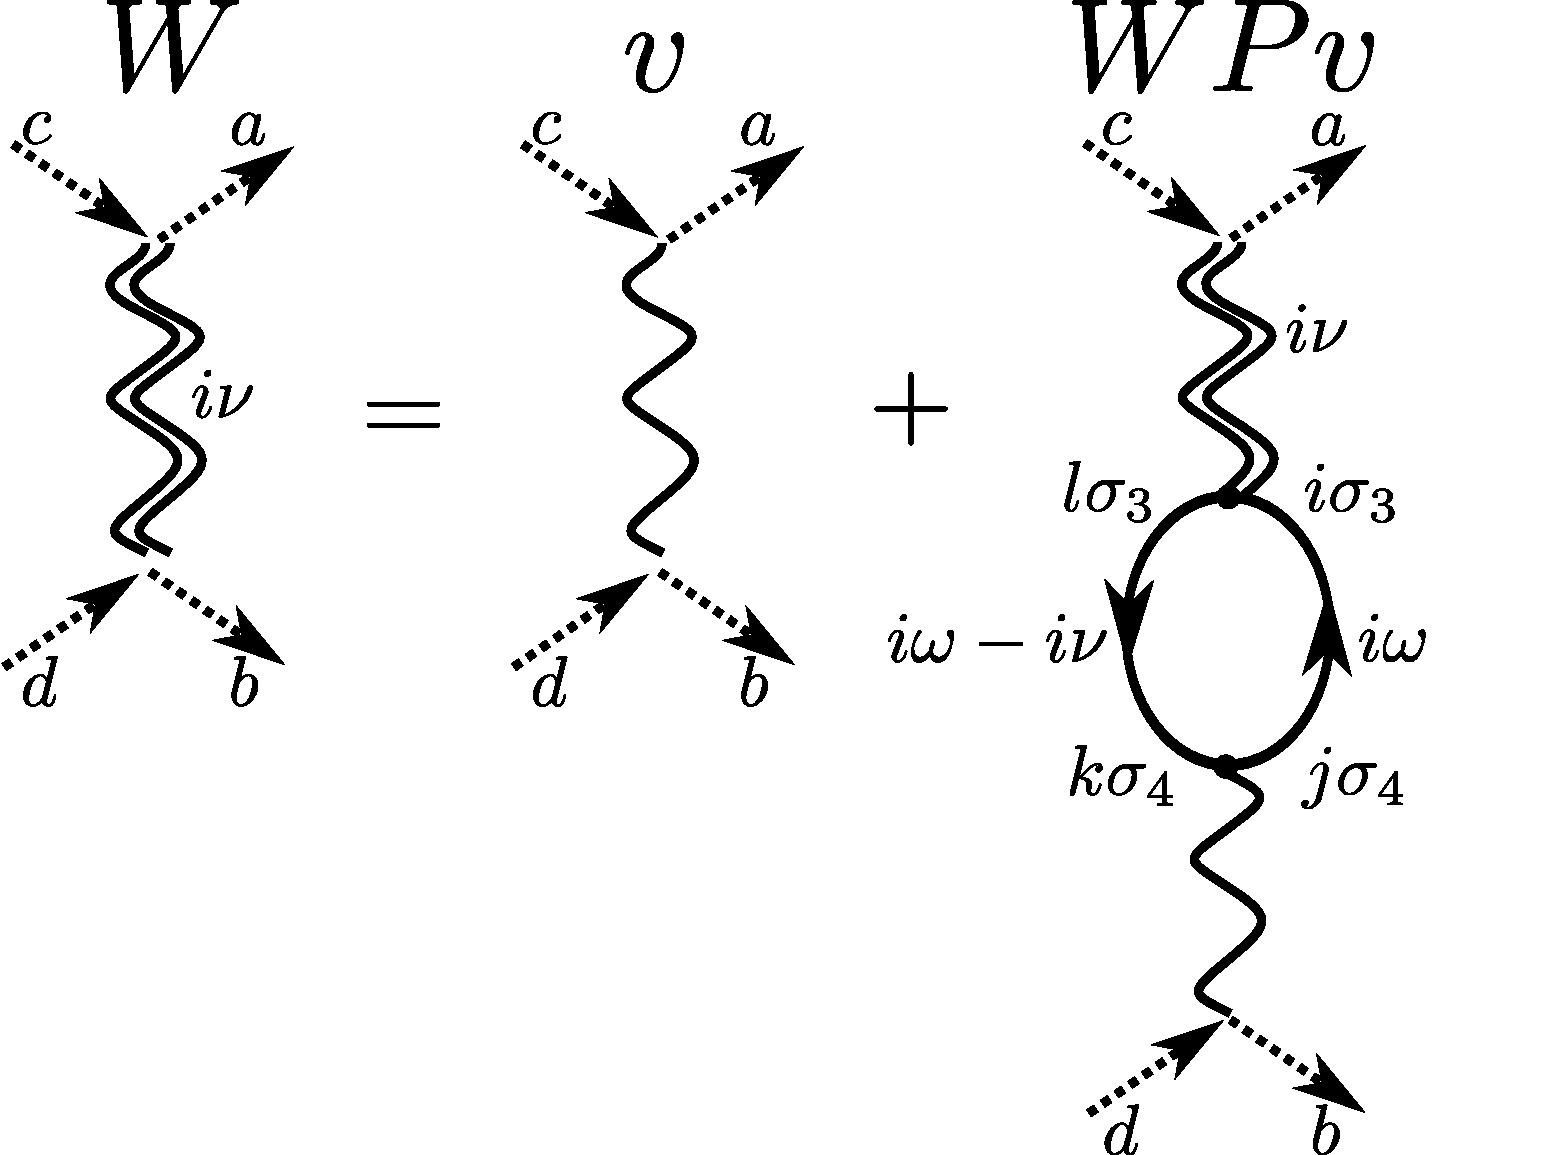
\includegraphics[width=0.55\textwidth]{figs/rpa_diag.pdf}
\end{center}
\caption{The screened interaction $W=v+WPv$, calculated within the RPA approximation,
where the bare Coulomb interaction $v$ is screened by the polarization bubble
$P=GG$.}
\label{fig:w_rpa}
\end{figure}
%%%%%%%%%%%%%%%%%%%%%%%%%%%%%%%%%%%%%%%%%%%%%%%%%%%%%%%%%%%%%%%%%%%%%%%%%%%%%

From this expression we \textit{define} the coefficients of  polarization $P$ in
the local basis as
\begin{align}
 P^{\sigma\sigma'}_{ijkl}(\tau,\tau') 
 &:= G^{\sigma\sigma'}_{ij}(\tau,\tau') G^{\sigma'\sigma}_{lk}(\tau',\tau),
\end{align}
which leads to the expression
\begin{align}
W_{abcd}(\tau_1,\tau_2) 
%
&= v_{abcd}(\tau_1,\tau_2)  \nonumber \\ 
& \hspace{0.5cm}  + \sum_{\substack{\sigma_3\sigma_4 \\ ijkl }}\int 
                     W_{alci}(\tau_1,\tau_3) 
                     P^{\sigma_3\sigma_4}_{ijlk}(\tau_3,\tau_4) 
                     v_{jbkd}(\tau_4,\tau_2)
                    \, \mathrm{d}\tau_3\mathrm{d}\tau_4 .
%
\end{align}
Other definitions of the $P_{ijkl}$ elements are possible and can be found in the literature.
The only thing important is that the notation is consistent.

Assuming spin-diagonal Green's functions, we can simplify the summation
over spins and redefine the polarization
\begin{align}
 P_{ijkl}(\tau,\tau') 
 &=\sum_{\sigma\sigma'} \delta_{\sigma\sigma'}G^{\sigma\sigma'}_{ij}(\tau,\tau') G^{\sigma'\sigma}_{lk}(\tau',\tau) \\
 &=\sum_{\sigma} G^{\sigma}_{ij}(\tau,\tau') G^{\sigma}_{lk}(\tau',\tau) ,
\end{align}
which leads to the final expression
\begin{align}
W_{abcd}(\tau_1,\tau_2) 
%
&= v_{abcd}(\tau_1,\tau_2)  \nonumber \\ 
& \hspace{0.5cm}  + \sum_{ijkl}\int 
                     W_{alci}(\tau_1,\tau_3) 
                     P_{ijlk}(\tau_3,\tau_4) 
                     v_{jbkd}(\tau_4,\tau_2)
                    \, \mathrm{d}\tau_3\mathrm{d}\tau_4 .
%
\end{align}
This is the form we will use from now on.

%%%%%%%%%%%%%%%%%%%%%%%%%%%%%%%%%%%%%%%%%%%%%%%%%%%%%%%%%%%%%%%%%%%%%%%%%%%%%%%%%%

\subsection{The local $W_{abcd}$ and $P_{ijkl}$ on Matsubara frequencies}
\label{sec:local_w_p_matsubara}
Using the definition of the Fourier transform
\begin{align}
 F(\tau)   &= \frac{1}{\beta} \sum_{i\nu_n} F(i\nu_n)\mathrm{e}^{-i\nu_n\tau} \\
 F(i\nu_n) &= \int_{0}^{\beta} F(\tau)\mathrm{e}^{i\nu_n\tau} \, \mathrm{d}\tau,
\end{align}
and exploiting time-translational invariance of $W,v,P$, e.g.
\begin{align}
 W(\tau_1,\tau_2) = W(\tau_1-\tau_2) = W(\tau),
\end{align}
we first get the usual Dyson-like equation (good exercise, it's not difficult)
\begin{align}
W_{abcd}(i\nu_n)
%
&= v_{abcd}  + \sum_{ ijkl }
                     W_{alci}(i\nu_n) P_{ijlk}(i\nu_n)
                     v_{jbkd}, \label{eq:w_dyson_like}
\end{align}
where we have used that the bare Coulomb interaction is static
\begin{align}
 v(r_1\tau_1,r_2\tau_2) &= v(r_1,r_2) \delta(\tau_1-\tau_2).
\end{align}
For the polarization we get
\begin{align}
 P_{ijkl}(i\nu_n)
 &= \sum_{\sigma}\int_{0}^{\beta} \frac{1}{\beta^2}
      \left( \sum_{i\omega_n} G^{\sigma}_{ij}(i\omega'_n) \mathrm{e}^{-i\omega_n\tau} \right)
      \left( \sum_{i\omega'_n} G^{\sigma}_{lk}(i\omega'_n) \mathrm{e}^{+i\omega'_n\tau} \right)
      \mathrm{e}^{i\nu_n\tau} \, \mathrm{d}\tau  \\
%
 &= \sum_{\sigma}\sum_{\substack{i\omega_n\\i\omega'_n}} G^{\sigma}_{ij}(i\omega_n)
                                            G^{\sigma}_{lk}(i\omega_n')
      \frac{1}{\beta^2} \int_{0}^{\beta} \mathrm{e}^{i(\nu_n+\omega_n'-\omega_n) \tau}   \, \mathrm{d}\tau  \\
%
 &=\frac{1}{\beta} \sum_{\sigma,i\omega_n} G^{\sigma}_{ij}(i\omega_n)
                     G^{\sigma}_{lk}(i\omega_n-i\nu_n).
\end{align}




\subsection{Relation between the local $U_{ab}$, $J_{ab}$ and $W_{abcd}$ and $P_{ijkl}$ }
\label{sec:local_gw_form_matsubara}

In general we want to calculate the screened interaction $W$ from 
a Dyson-like equation by inverting Eq.~\ref{eq:w_dyson_like}
\begin{align}
 W &= [v^{-1} - P ]^{-1}.
\end{align}
In general one needs to employ a product basis ansatz
to invert the 4-index objects like described in Sec.~\ref{sec:product_basis}.
However, in practice when we want to obtain the polarization of the impurity
model within the RPA approximation there are significant simplifications.

First, we assume the local Green's functions to be spin- and orbital diagonal, i.e.
\begin{align}
 G^{\sigma\sigma'}_{ij}(i\omega_n)
 &= G^{\sigma}_{i}(i\omega_n)\delta_{\sigma\sigma'}\delta_{ij}.
\end{align}
Second, if we assume that only the Hubbard and Hund's terms of the local interaction
\begin{align}
 U^{\mathrm{bare}}_{ab} &= \braket{ab|v|ab} = v_{abab} \\
 J^{\mathrm{bare}}_{ab} &= \braket{ab|v|ba} = v_{abba} ,
\end{align}
are relevant and all other terms are sufficiently small, like 
we do in a standard Hubbard model DMFT calculation, the screened interaction parameters can be written as
\begin{align}
U^{\mathrm{scr}}_{ab}(i\nu_n) &= W_{abab}(i\nu_n) \\
%
&= v_{abab}  + \sum_{ i k }
                     W_{akai} (i\nu_n) P_{iikk}(i\nu_n)
                     v_{ibkb}\delta_{ik} \\
%
& = U^{\mathrm{bare}}_{ab}  + \sum_{i}
                     U^{\mathrm{scr}}_{ai} (i\nu_n) P_{iiii}(i\nu_n)
                     U^{\mathrm{bare}}_{ib} , 
\end{align}
and 
\begin{align}
J^{\mathrm{scr}}_{ab}(i\nu_n) &= W_{abba}(i\nu_n) \\
%
&= v_{abba}  + \sum_{ i k}
                     W_{akbi} (i\nu_n) P_{iikk}(i\nu_n)
                     v_{ibka}\delta_{ia}\delta_{kb} \\
%
& = J^{\mathrm{bare}}_{ab}  + 
                     J^{\mathrm{scr}}_{ab} (i\nu_n) P_{aabb}(i\nu_n)
                     J^{\mathrm{bare}}_{ab} \mbox{ , for } a\neq b \mbox{ !}
\end{align}
The equation for $U^{\mathrm{scr}}_{ab}$ has now been reduced to a simple matrix equation
\begin{align}
U^{\mathrm{scr}}(i\nu_n) 
& = U^{\mathrm{bare}}  + U^{\mathrm{scr}} (i\nu_n) P^{\mathrm{diag}}(i\nu_n) U^{\mathrm{bare}},
\end{align}
where $P^{\mathrm{diag}}$ is a diagonal matrix consisting of the $P_{iiii}$ elements 
\begin{align}
 P^{\mathrm{diag}}_{ab}(i\nu_n) &=  P_{aaaa}(i\nu_n) \delta_{ab}.
\end{align}
The equation for $J^{\mathrm{scr}}_{ab}$ has even become a simple scalar equation.
These relations can be easily inverted, which finally yields the expressions
\begin{align}
 U^{\mathrm{scr}}_{ab}(i\nu_n) 
 &= \left( U^{\mathrm{bare}} \left[\unity -  P^{\mathrm{diag}}(i\nu_n) U^{\mathrm{bare}} \right]^{-1} \right)_{ab} \\
 &=  \left( \left[ \left(U^{\mathrm{bare}}\right)^{-1} -  P^{\mathrm{diag}}(i\nu_n) \right]^{-1} \right)_{ab} \\
 %
 J^{\mathrm{scr}}_{ab}(i\nu_n) 
 &= \frac{ J^{\mathrm{bare}}_{ab} }{ 1 - P_{ab}(i\nu_n)J^{\mathrm{bare}}_{ab} }  \\
 &= \left[  \left(J^{\mathrm{bare}}_{ab} \right)^{-1} - P_{ab}(i\nu_n) \right]^{-1} \mbox{ for } a\neq b,
\end{align}
where  $P_{ab} = P_{aabb}$, and the inverse in the equation for $U^{\mathrm{scr}}$
is defined as the standard matrix inverse. In the equation for $J^{\mathrm{scr}}$ it is just 
a scalar inverse.

Inverting the equations for the bare values one obtains the corresponding expressions
\begin{align}
 U^{\mathrm{bare}}_{ab}
 &= \left( \left[\unity + U^{\mathrm{scr}}(i\nu_n) P^{\mathrm{diag}}(i\nu_n) \right]^{-1} U^{\mathrm{scr}}(i\nu_n) \right)_{ab} \\
 &=  \left( \left[ \left(U^{\mathrm{scr}}(i\nu_n)\right)^{-1} +  P^{\mathrm{diag}}(i\nu_n) \right]^{-1} \right)_{ab} \\
 %
 J^{\mathrm{bare}}_{ab} 
 &= \frac{ J^{\mathrm{scr}}_{ab}(i\nu_n) }{ 1 + J^{\mathrm{scr}}_{ab}(i\nu_n) P_{ab}(i\nu_n) } \\
 &= \left[  \left(J^{\mathrm{scr}}_{ab}(i\nu_n) \right)^{-1} + P_{ab}(i\nu_n) \right]^{-1} \mbox{ for } a\neq b.
\end{align}

The elements of the local polarization that are relevant can be 
calculated as
\begin{align}
 P_{aa}(i\nu_n)  
 &= \left[ \left(U^{\mathrm{bare}}\right)^{-1} - \left(U^{\mathrm{scr}}(i\nu_n)\right)^{-1} \right]_{aa} \\
%
 P_{ab}(i\nu_n) 
 &= \frac{1}{J^{\mathrm{bare}}_{ab}} - \frac{1}{J^{\mathrm{scr}}_{ab}(i\nu_n)} \mbox{ for } a\neq b.
\end{align}
\textbf{Attention:} This is valid only if no approximation is made on the frequency dependence
of the interaction! If $J^{\mathrm{scr}}$ is taken from the impurity model
considering only $F_0$ screening this equation is obviously not valid!

\subsection{Obtaining $W(i\nu_n)$ and $P(i\nu_n)$ of the impurity from 
the charge-charge correlation function  $\chi_{ij}$}
In the GW+DMFT cycle we have to update the local polarization $P$
from the GW with the DMFT polarization.
The relations between the fully screened interaction $W(i\nu_n)$, the partially
screened interaction $U(i\nu_n)$, the Polarization $P(i\nu_n)$ and the charge-susceptibility
$\chi^{ch}(i\nu_n)$ is as follows:
\begin{align}
 U(i\nu_n) &= \left[  W^{-1}(i\nu_n) + P(i\nu_n)  \right]^{-1} \\
 W(i\nu_n) &= U(i\nu_n) -U(i\nu_n) \chi^{ch}(i\nu_n)U(i\nu_n)  \\
 P(i\nu_n) &= -\left[ \unity - \chi^{ch}(i\nu_n)U(i\nu_n) \right]^{-1} \chi^{ch}(i\nu_n) \\
           &= \left[ U(i\nu_n) - \chi^{-1}_{ch}(i\nu_n) \right]^{-1}.
\end{align}
The charge susceptibility $\chi^{ch}$ is given by
\begin{align}
 \chi^{ch}_{ij}(\tau) 
 &= \langle T \bar{n}_i(\tau) \bar{n}_j(0) \rangle ,
\end{align}
where $\bar{n}_i(\tau) = \sum_{\sigma} \left( n^{\sigma}_i(\tau) - \langle n^{\sigma}_i\rangle \right)$.

In the impurity solver we can measure the time-dependent density-density
correlation function $\chi_{ij}^{\sigma\sigma'}(\tau)$ given by
\begin{align}
 \chi_{ij}^{\sigma\sigma'}(\tau) 
 &= \langle T n_i^{\sigma}(\tau) n_j^{\sigma'}(0) \rangle \\
 %
 \chi_{ij}^{\sigma\sigma'}(i\nu_n) 
 &= \int_0^{\beta} \chi_{ij}^{\sigma\sigma'}(\tau) \mathrm{e}^{i\nu_n\tau} \,\mathrm{d}\tau.
\end{align}
This is a bosonic response function and real-valued on the imaginary $\tau$- and $i\nu_n$ axis.

The charge-susceptibility $\chi^{ch}(i\nu_n)$ can be expressed in terms of
the time-dependent density-density correlation function $\chi$ by
\begin{align}
 \chi^{ch}_{ij}(\tau) 
 &= \langle T \bar{n}_i(\tau) \bar{n}_j(0) \rangle \\
 %
 &= \langle T \left( n_i(\tau)-\langle n_i \rangle \right) 
              \left( n_j(0)-\langle n_j \rangle \right)\rangle \\
 %
 &= \langle T \left( n_i(\tau)n_j(0) - n_i(\tau)\langle n_j \rangle
                                     - \langle n_i \rangle n_j(0)
                                     + \langle n_i \rangle\langle n_j \rangle
              \right)\rangle \\ 
 &= \langle T n_i(\tau)n_j(0) \rangle - \langle n_i \rangle\langle n_j \rangle \\
 %
 &= \langle T \left( n^{\uparrow}_i(\tau)+n^{\downarrow}_i(\tau) \right)
              \left( n^{\uparrow}_j(0)+n^{\downarrow}_j(0) \right)\rangle  \nonumber \\
 & \hspace{0.5cm}  -\langle n^{\uparrow}_i+n^{\downarrow}_i  \rangle\langle n^{\uparrow}_j+n^{\downarrow}_j  \rangle \\
 %
 &=  \chi_{ij}^{\uparrow\uparrow}(\tau) + \chi_{ij}^{\downarrow\downarrow}(\tau) 
    +\chi_{ij}^{\uparrow\downarrow}(\tau)  +\chi_{ij}^{\downarrow\uparrow}(\tau)  \nonumber \\
 & \hspace{0.3cm} - \left( \chi_{ii}^{\uparrow\uparrow}(0)+\chi_{ii}^{\downarrow\downarrow}(0)  \right)
                    \left( \chi_{jj}^{\uparrow\uparrow}(0)+\chi_{jj}^{\downarrow\downarrow}(0)  \right),
 \end{align}
 where we have used that 
 \begin{align}
  \chi_{ii}^{\sigma\sigma}(0) 
  &= \langle T n^{\sigma}_i(0) n^{\sigma}_i(0) \rangle \\
  &= \langle  n^{\sigma}_i(0) \rangle \\
  &= \langle n^{\sigma}_i \rangle.
 \end{align}
Using the Fourier transform we get the charge susceptibility on the Matsubara
frequency axis
\begin{align}
 \chi^{ch}_{ij}(i\nu_n) 
 &=   \chi_{ij}^{\uparrow\uparrow}(i\nu_n) + \chi_{ij}^{\downarrow\downarrow}(i\nu_n) 
    +\chi_{ij}^{\uparrow\downarrow}(i\nu_n)  +\chi_{ij}^{\downarrow\uparrow}(i\nu_n) \nonumber \\
 & \hspace{0.3cm} - \delta(i\nu_n) \beta \langle n^{\uparrow}_i+n^{\downarrow}_i  \rangle\langle n^{\uparrow}_j+n^{\downarrow}_j  \rangle.
\end{align}


We will now derive the relation between the screened interaction $W$ and the density-density
correlation function $\chi$, starting from the general equation
\begin{align}
W(1,2)
&=v(1,2) - \int v(1,2) \braket{T\rho'(3)\rho'(4)} v(4,2) \, \mathrm{d}(3)\mathrm{d}(4), 
\end{align}
where
\begin{align}
 \rho'(1) &= \psi^{\dagger}(1)\psi(1) - \braket{ \psi^{\dagger}(1)\psi(1) }.
\end{align}
Introducing a local basis $\chi^{\sigma}_m(r)$ and expanding the density operators as
\begin{align}
\rho(r\sigma\tau) &= \sum_{ij} \chi^{\sigma}_i(r) \rho^{\sigma}_{ij}(\tau) \chi^{*\sigma}_j(r),
\end{align}
we obtain the matrix element
\begin{align}
W_{abcd}(\tau_1,\tau_2) 
&= v_{abcd}(\tau_1,\tau_2)  
- \int \chi^{*\sigma}_a(r_1)\chi^{*\sigma'}_b(r_2) v(r_1\tau_1,r_3\tau_3)   \nonumber \\
            & \hspace{3cm} \times \braket{T\rho'(r_3\sigma_3\tau_3)\rho'(r_4\sigma_4\tau_4)}
                            v(r_4\tau_4,r_1\tau_1) \chi^{\sigma''}_c(r_1)\chi^{\sigma'''}_d(r_2) \nonumber \\
            &\hspace{3cm} \times \chi^{\sigma''}_c(r_1)\chi^{\sigma'''}_d(r_2)
                                             \, \mathrm{d}(3)\mathrm{d}(4) \mathrm{d}r_1 \mathrm{d}r_2 \\
%
&= v_{abcd}(\tau_1,\tau_2)  
- \sum_{ijkl}\int \chi^{*\sigma}_a(r_1)\chi^{*\sigma'}_b(r_2)
                                    v(r_1\tau_1,r_3\tau_3) \chi^{\sigma_3}_i(r_3) \chi^{*\sigma_3}_j(r_3) \nonumber\\
               &\hspace{3cm} \times   \braket{T\rho'^{\sigma_3}_{ij}(\tau_3)\rho'^{\sigma_4}_{kl}(\tau_4)}
                            \chi^{\sigma_4}_k(r_4) \chi^{*\sigma_4}_l(r_4)
                            v(r_4\tau_4,r_1\tau_1)                                         \nonumber \\
               &\hspace{3cm} \times  \chi^{\sigma''}_c(r_1)\chi^{\sigma'''}_d(r_2)
                                                        \, \mathrm{d}(3)\mathrm{d}(4) \mathrm{d}r_1 \mathrm{d}r_2 \\
%
&= v_{abcd}(\tau_1,\tau_2)  
- \sum_{\substack{ijkl\\ \sigma_3\sigma_4}}\int v_{ajci}(\tau_1,\tau_3)  \braket{T\rho'^{\sigma_3}_{ij}(\tau_3)\rho'^{\sigma_4}_{kl}(\tau_4)}    \nonumber\\
               &\hspace{3cm} \times   v_{lbkd}(\tau_4,\tau_1)   \, \mathrm{d}\tau_3 \mathrm{d}\tau_4 .
\end{align}
Please note that we keep the general time/frequency dependence of the unscreened interaction
$v_{abcd}(\tau_1,\tau_2)$, since this will usually correspond to the effective dynamical
impurity interaction.

Since we work with the charge density-density correlation function, we use
\begin{align}
\sum_{\sigma_3\sigma_4} \braket{T\rho'^{\sigma_3}_{ij}(\tau_3)\rho'^{\sigma_4}_{kl}(\tau_4)}
 &= \chi^{ch}_{ik}(\tau_3,\tau_4) \delta_{ij} \delta_{kl},
\end{align}
and after a Fourier transform, using time-translational invariance, we obtain
\begin{align}
W_{abcd}(i\nu_n) 
%
&= v_{abcd}(i\nu_n)  
- \sum_{ik} v_{aici}(i\nu_n)  \chi^{ch}_{ik}(i\nu_n)  v_{kbkd}(i\nu_n) .
\end{align}
If we now assume that only the Hubbard- and Hund's terms are relevant
\begin{align}
 U^{bare}_{ab}(i\nu_n) &= v_{abab}(i\nu_n) \\
 J^{bare}_{ab}(i\nu_n) &= v_{abba}(i\nu_n),
\end{align}
and neglect all others, we obtain
\begin{align}
U^{scr}_{ab}(i\nu_n) 
&= U^{bare}_{ab}(i\nu_n) - \sum_{ij} U^{bare}_{ai}(i\nu_n)  \chi^{ch}_{ij}(i\nu_n)  U^{bare}_{jb}(i\nu_n) \\
%
J^{scr}_{ab}(i\nu_n) 
&= J^{bare}_{ab}(i\nu_n) - \sum_{ij} v_{aibi}(i\nu_n)  \chi^{ch}_{ij}(i\nu_n)  v_{jbja}(i\nu_n) \nonumber \\
&= J^{bare}_{ab}(i\nu_n) \ \ \forall a\neq b.
\end{align}
This means by using only the charge density-density correlation function
there is no screening of the Hund's terms!
These equations now have become standard matrix multiplications
\begin{align}
U^{scr}_{ab}(i\nu_n) 
&= U^{bare}_{ab}(i\nu_n) - \left[ U^{bare}(i\nu_n)  \chi^{ch}(i\nu_n)  U^{bare}(i\nu_n) \right]_{ab} \\
%
J^{scr}_{ab}(i\nu_n) 
&= J^{bare}_{ab}(i\nu_n) \ \ \forall a\neq b.
\end{align}
Using the equation for the polarization that was derived in Chapter~\ref{sec:glocwloc_dc_factor}
under the same assumptions, we get for the impurity case
\begin{align}
 P^{imp}_{aa}(i\nu_n) &= \left[ U^{bare}(i\nu_n) \right]^{-1}_{aa} 
                           - \left[ U^{bare}(i\nu_n)\chi(i\nu_n)U^{bare}(i\nu_n) \right]^{-1}_{aa} \nonumber \\
                      &= \left[ U^{bare}(i\nu_n) - (\chi^{ch}(i\nu_n))^{-1} \right]^{-1}_{aa} \\
%
 P^{imp}_{ab}(i\nu_n) &= 0 \ \ \forall a\neq b.
\end{align}
This last equation for offdiagonal components of the polarization 
are quite interesting. They vanish since there is no screening from 
the charge density-density correlation function on the Hund's coupling terms.
Therefore, special care should be taken when replacing the local part
of the GW polarization by the impurity polarization. Should we keep the offdiagonal
components from the RPA polarization or should we just set them to zero?
The question is whether the RPA result is more correct than simply neglecting these terms.
It should be quite obvious that exactly zero is not physical since the Hund's terms
are screened. But maybe the RPA overestimates this screening significantly and 
an approximation by zero is still better?
This needs to be discussed.



%%%%%%%%%%%%%%%%%%%%%%%%%%%%%%%%%%%%%%%%%%%%%%%%%%%%%%%%%%%%%%%%%%%%%%%%%%
%%%%%%%%%%%%%%%%%%%%%%%%%%%%%%%%%%%%%%%%%%%%%%%%%%%%%%%%%%%%%%%%%%%%%%%%%%
%%%%%%%%%%%%%%%%%%%%%%%%%%%%%%%%%%%%%%%%%%%%%%%%%%%%%%%%%%%%%%%%%%%%%%%%%%
%%%%%%%%%%%%%%%%%%%%%%%%%%%%%%%%%%%%%%%%%%%%%%%%%%%%%%%%%%%%%%%%%%%%%%%%%%
%%%%%%%%%%%%%%%%%%%%%%%%%%%%%%%%%%%%%%%%%%%%%%%%%%%%%%%%%%%%%%%%%%%%%%%%%%
%%%%%%%%%%%%%%%%%%%%%%%%%%%%%%%%%%%%%%%%%%%%%%%%%%%%%%%%%%%%%%%%%%%%%%%%%%

\section{The GW+DMFT Doublecounting}
In the section above we discussed that the "doublecounting" factor
that has to be subtracted from the GW Selfenergy and Polarization
should be 
\begin{align}
\Sigma^{GW,DC} &= -G^{0,\mathrm{loc},L}W^{0,\mathrm{loc},L} \\
P^{GW,DC} &= G^{0,\mathrm{loc},L}G^{0,\mathrm{loc},L}
\end{align}
This method using $\Sigma^{GW,DC} = -G^{0,\mathrm{loc},L}W^{0,\mathrm{loc},L}$
can be understood as calculating a GW Selfenergy excluding any contributions arising
exclusively in the correlated subspace, and then adding the contributions arising only in
the correlated subspace via DMFT. 

Other choices have been discussed, for example what we have been using previously
is to subtract all local terms from GW
\begin{align}
\Sigma^{GW,DC^*} &= -[G^{0}W^{0}]^{\mathrm{loc},L} = \frac{1}{N_k}\sum_k \Sigma^{GW,L}  \\
P^{GW,DC^*} &= [G^{0}G^{0}]^{\mathrm{loc},L} = \frac{1}{N_k}\sum_k P^{GW,L}
\end{align}
IMPORTANT: These two doublecounting factors are not equal as long as we restrict 
to a smaller subspace $L$, since the local component of the Selfenergy and Polarization
contain terms arising from the interaction with the smaller subspace $L$
and the remaining part $R = H \setminus L$
\begin{align}
\Sigma^{GW,loc} &= -G_{LL}^{0,\mathrm{loc}}W^{0,\mathrm{loc}}_{LL}
                   -G^{0,\mathrm{loc}}_{RR}W^{0,\mathrm{loc}}_{LRRL}
\end{align}
Only when $L=H$ is the full Hilbert space, they are equal since the second term
is also included. This problem does not arise for the polarization, since
there is no four-index object like $W$ which couples the two spaces.

\begin{figure}[t]
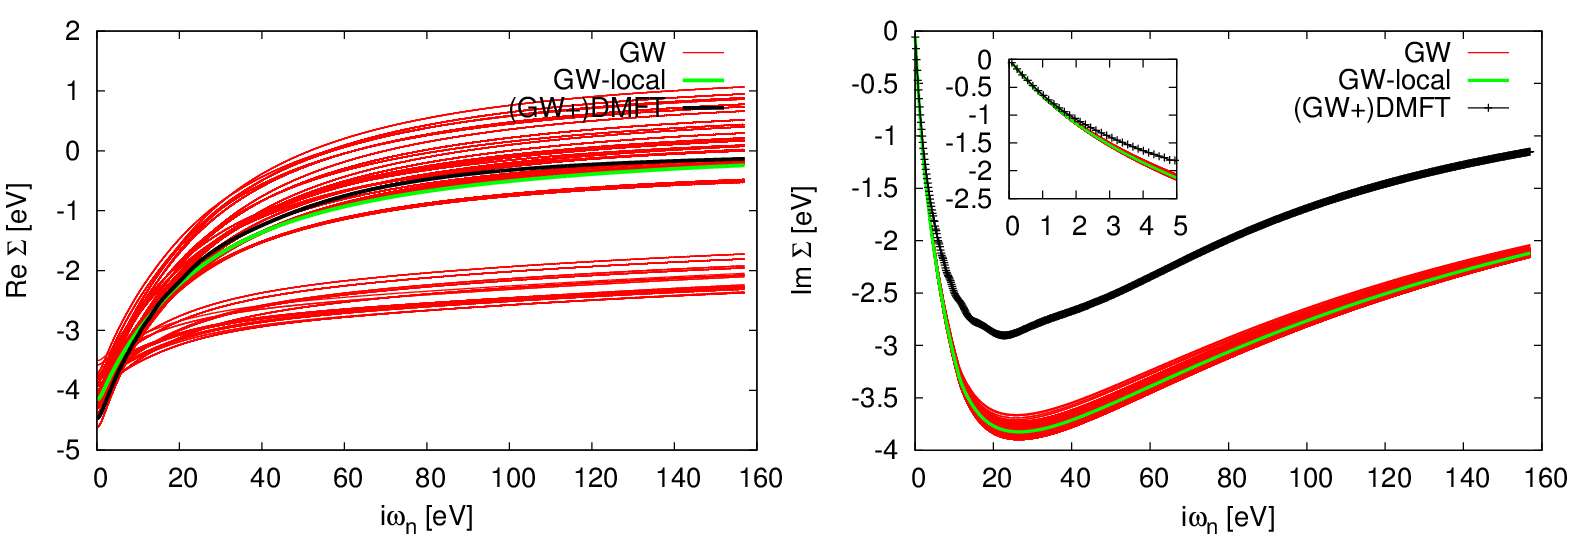
\includegraphics[width=1.0\textwidth]{figs/sigma_loc_compare.png}
\caption{The Selfenergy $\Sigma(i\omega_n)$ obtained from G$_0$W$_0$ (7x7x7 k-points)
 and GW+DMFT using the G$_0$W$_0$ input for a $t_{2g}$-only model for SrVO$_3$ 
 with $U(\omega)$ interaction determined from cRPA. As the doublecounting
 $\Sigma_{GW}^{DC}$ the local part of the GW Selfenergy $\sum_k GW$ on the
 correlated orbitals been subtracted (green line, called GW-local).
 One clearly sees a mismatch between this term and the DMFT Selfenergy (black line),
 which is due to the terms contributing to the local Selfenergy that arise
 from the coupling between the subspace and the remaining states and 
 also the nonlocal contributions to the local part which cannot be captured by DMFT.
}
\label{fig:sigma_loc_compare}
\end{figure}

In Fig.\ref{fig:sigma_loc_compare} we show a comparison between the Selfenergy 
$\Sigma(i\omega_n)$ obtained from a G$_0$W$_0$ (7x7x7 k-points) calculation,
and GW+DMFT using the G$_0$W$_0$ input for a $t_{2g}$-only model for SrVO$_3$ with $U(\omega)$ interaction determined from cRPA.
The GW-local is the k-averaged part of the GW Selfenergy, and the GW+DMFT Selfenergy
is the local Selfenergy of the impurity model
after convergence of the GW+DMFT cycle including the non-local components
of the GW Selfenergy but subtracting the GW-local part as the doublecounting.
This means we have thrown away all contributions $G^{0,\mathrm{loc}}_{RR}W^{0,\mathrm{loc}}_{LRRL}$
arising from the interaction between the correlated subspace and the rest.

The discrepancy between the impurity Selfenergy and the k-averaged
GW Selfenergy, that can be seen especially in the imaginary part,
can then in principle have to reasons:

One contribution will be the contributions from the subspace
with the rest $G^{0,\mathrm{loc}}_{RR}W^{0,\mathrm{loc}}_{LRRL}$, as already discussed.
Another contribution can arise from the cRPA screening to obtain the effective
interaction $U(\omega)$. If the bare value is not the proper one, this would also
lead to a discrepancy especially in the tail sections of the Selfenergy, i.e.
if the value is too small, the tail will be smaller. 

\textbf{PLEASE NOTE:}
The GW doublecounting factor $\Sigma^{GW,DC}$ should not contain the Hartree
part, since the GW Selfenergy $\Sigma^{GW}_{XC}$ does not contain it.

First tests using both methods in SrVO3 show that $-G^{0,\mathrm{loc},L}W^{0,\mathrm{loc},L}$
seems to reduce the rernormalization in the unoccupied part.
With the other DC there seemed to be a shift in the chemical potential where
the bands are slightly too low, but the reason for this is not fully clear and
maybe something else might be responsible, but I don't think so.

%%%%%%%%%%%%%%%%%%%%%%%%%%%%%%%%%%%%%%%%%%%%%%%%%%%%%%%%%%%%%%%%%%%%%%%%%%
%%%%%%%%%%%%%%%%%%%%%%%%%%%%%%%%%%%%%%%%%%%%%%%%%%%%%%%%%%%%%%%%%%%%%%%%%%

\subsection{Different variants of $W_{\mathrm{loc}}$}
In order to evaluate the doublecounting factor
\begin{align}
\Sigma^{DC}_{GW} &= -[G^{\mathrm{loc}}W^{\mathrm{loc}}],
\end{align}
we will solve the impurity model within the $G_0W_0$ approximation.
Therefore, $G^{\mathrm{loc}}=G^{\mathrm{loc}}_{\mathrm{DFT}}$.
But what one should use for $W^{\mathrm{loc}}$ is not trivial.

There are basically two options one could use
\begin{itemize}
 \item Calculate $W(r,r')$ in the GW calculation and project it
 onto the localized basis set. This object is then used to calculate the 
 doublecounting (This is what we have used so far).
 This is in priniciple not correct, since the impurity problem
 only knows about the effective impurity interaction $U$, that is then
 screened by local processes, while such a $W$ from GW contains in general
 different screening processes (see discussion also below):
 
 Usually the cRPA calculation for $U$ is done by excluding the correlated bands 
 from the screening process, so non-local processes in these bands are removed as well.
 These processes are not accounted for in the impurity model. If we use the fully screened
 $W$ from the GW calculation these processes are included, so this $W$ will obviously
 be different from $[U^{-1} - P_{\mathrm{loc}} ]^{-1}$. 
 
 \item The other way is to use the effective impurity interaction $U$, calculate
 the polarization of the impurity in GW from the DFT input via
 $P_{\mathrm{loc}} = G_{\mathrm{loc}}G_{\mathrm{loc}}$ and screen the interaction
 via $W_{\mathrm{loc}} = [U^{-1} - P_{\mathrm{loc}} ]^{-1}$.
 This corresponds to a GW solution of the impurity model and the DMFT solution should
 recover this GW solution if correlations are weak. 
\end{itemize}

Another point to this discussion:
First, the following identity
\begin{align}
 \left[ GG \right]_{\mathrm{loc}} = G_{\mathrm{loc}}G_{\mathrm{loc}},
\end{align}
tells us that the local projection of the polarization is equal
to the polarization calculated from local quantities.
This means that either calculating $P$ in the continuum and then projecting
it onto the local basis, or first projecting the Green's function onto the local basis
and then calculating $P$ yields the same result. 

Therefore, if one would not adopt a cRPA procedure to calculate the effective $U$
but instead remove the local polarization $P$ (like one does in a full GW+DMFT selfconsistent scheme)
\begin{align}
 U^{-1}_{loc} = W^{-1}_{loc} + P_{loc},
\end{align}
there should be no difference in the procedure, because if we screen $U$ again by
the local RPA polarization we get back the local $W$ calculated from GW.

However,
this is in general not true since additional approximations on the effective
interaction are employed when constructing the impurity model.
We will only consider dynamical screening on the monopole term $F_0$
and neglect all higher orders. The $J_{ab}$ elements will therefore be constant
and usually taken as their zero frequency values.
As a result the local screened interaction $W^{-1}_{loc,eff}$ will be different 
from the projected screened interaction
\begin{align}
W^{-1}_{loc,eff} =  U^{-1}_{loc} - P_{loc} \neq \left[ v^{-1} - P \right]_{loc} = W^{-1}_{loc} 
\end{align}
since additional approximations on $U^{-1}_{loc}$ have been emplyed.
Therefore, it is in general important to calculate $W_{loc}$ used in the Doublecounting
directly from the final effective impurity interaction $U_{loc}$,
instead of taking the projected $W$ from the GW calculation.

\begin{figure}[t]
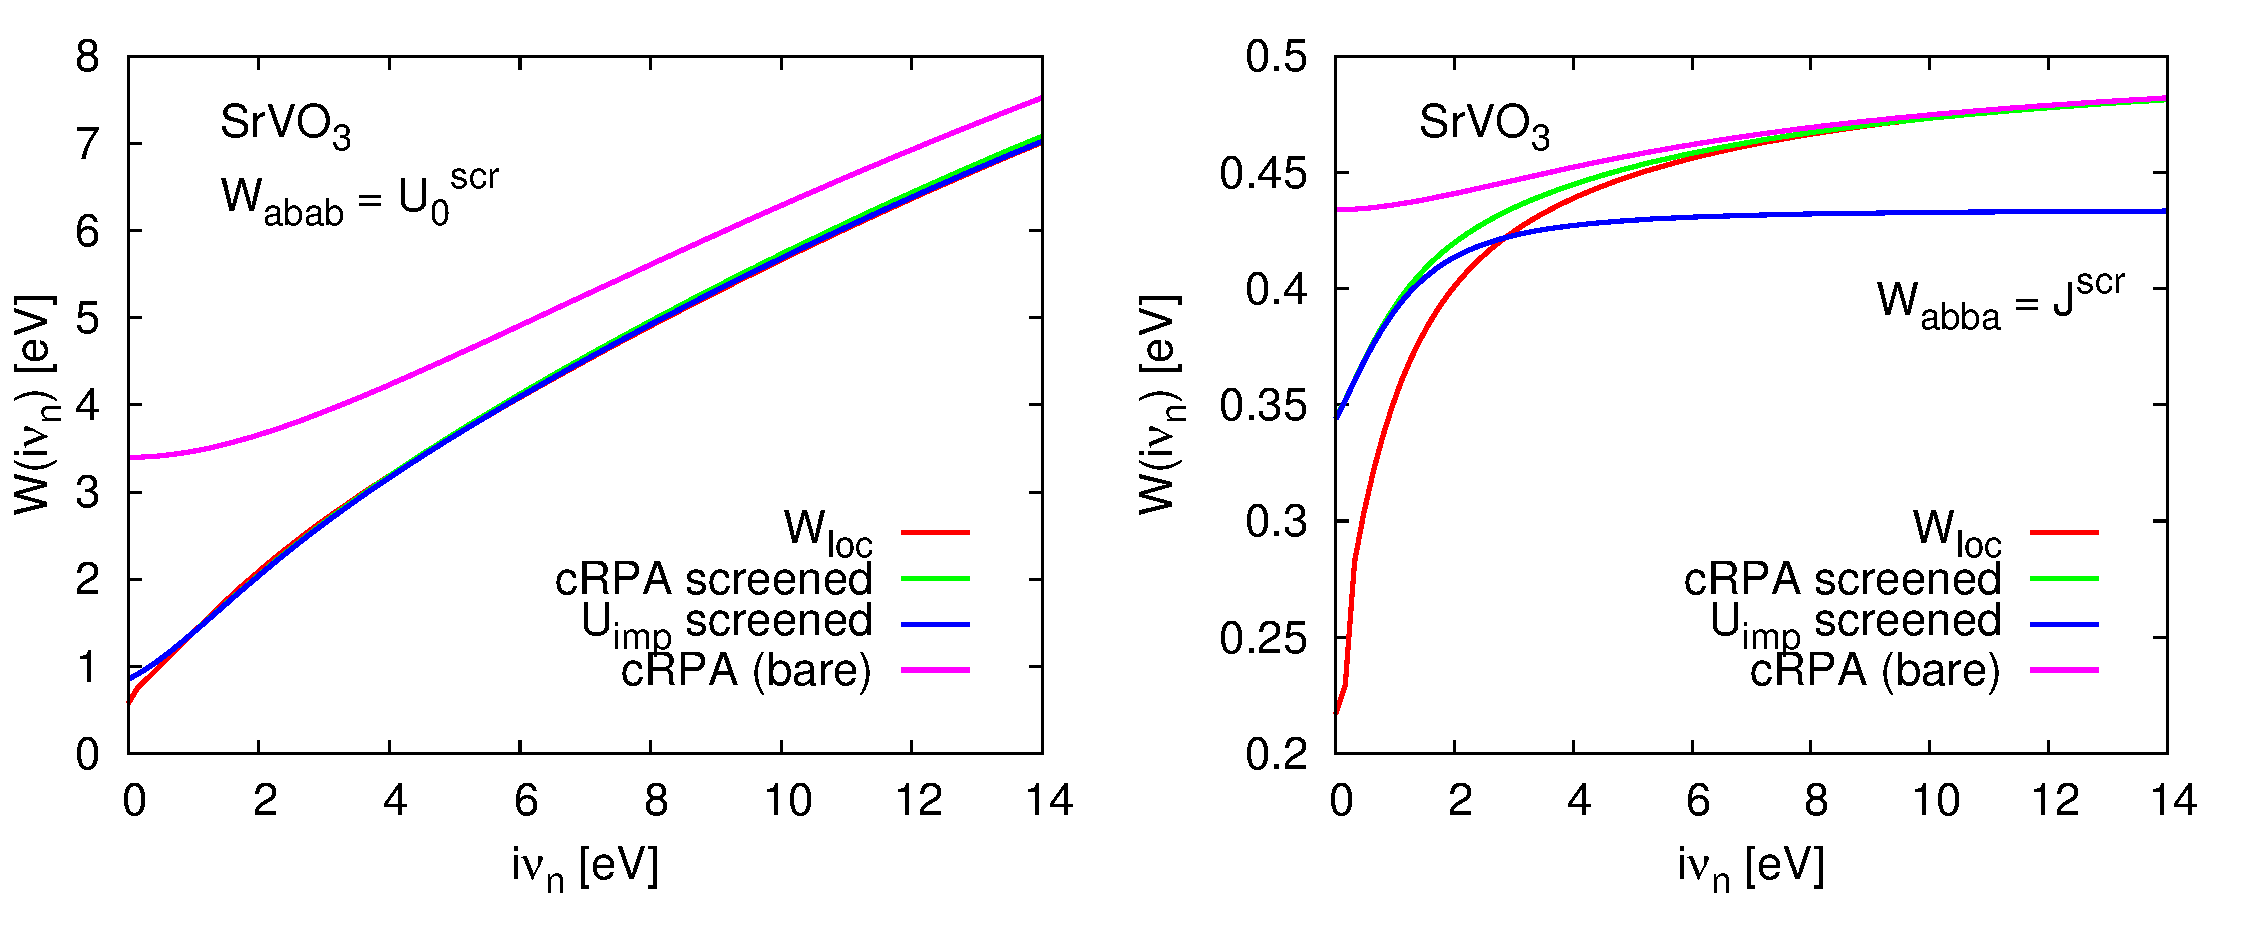
\includegraphics[width=1.0\textwidth]{figs/Wloc/W_loc_comp.pdf}
\caption{The bare and screened interaction parameters $U_0$ (left) and $J$ (right)
for the $t_{2g}$ orbitals in SrVO$_3$ on the Matsubara axis. 
cRPA (bare) indicates the effective bare value of the interaction
where transitions only in the $t_{2g}$ manifold have been removed, while $W_{loc}$
is the value including all transitions.
The cRPA screened values are obtained by screening the cRPA (bare) values by the local
polarization $P_{\mathrm{loc}}=G_{\mathrm{loc}}G_{\mathrm{loc}}$.
The $U_{\mathrm{imp}}$ values are obtained in the same way by starting from the effective impurity interaction
where only $F_0$ screening has been initially considered.
}
\label{fig:W_loc_comparison}
\end{figure}

A comparison between the different types of $W$ can be seen in Fig.~\ref{fig:W_loc_comparison}.
We observe that the local projection $W_{loc}$ is extremely close to the
bare cRPA interaction screened by the local RPA polarization $P_{\mathrm{loc}}=G_{\mathrm{loc}}G_{\mathrm{loc}}$.
This means that for the monopole terms of the interaction
the cRPA scheme of removing transitions between bands is basically identical
to the scheme of removing transitions between orbitals.

On the other hand, for the Hund's terms there is a siginificat deviation between the procedures,
where the local orbital-based screening obtains a much larger value.
This means that for the Hund's terms removing transitions between bands involves more
screening processes which are not originating from local transitions in the $t_{2g}$ orbitals.
Thus, eventually, the cRPA scheme yields a larger effective bare interaction 
for the impurity model, compared to removing the local polarization from the fully screened interaction.
This should be investigated further.

\begin{figure}[t]
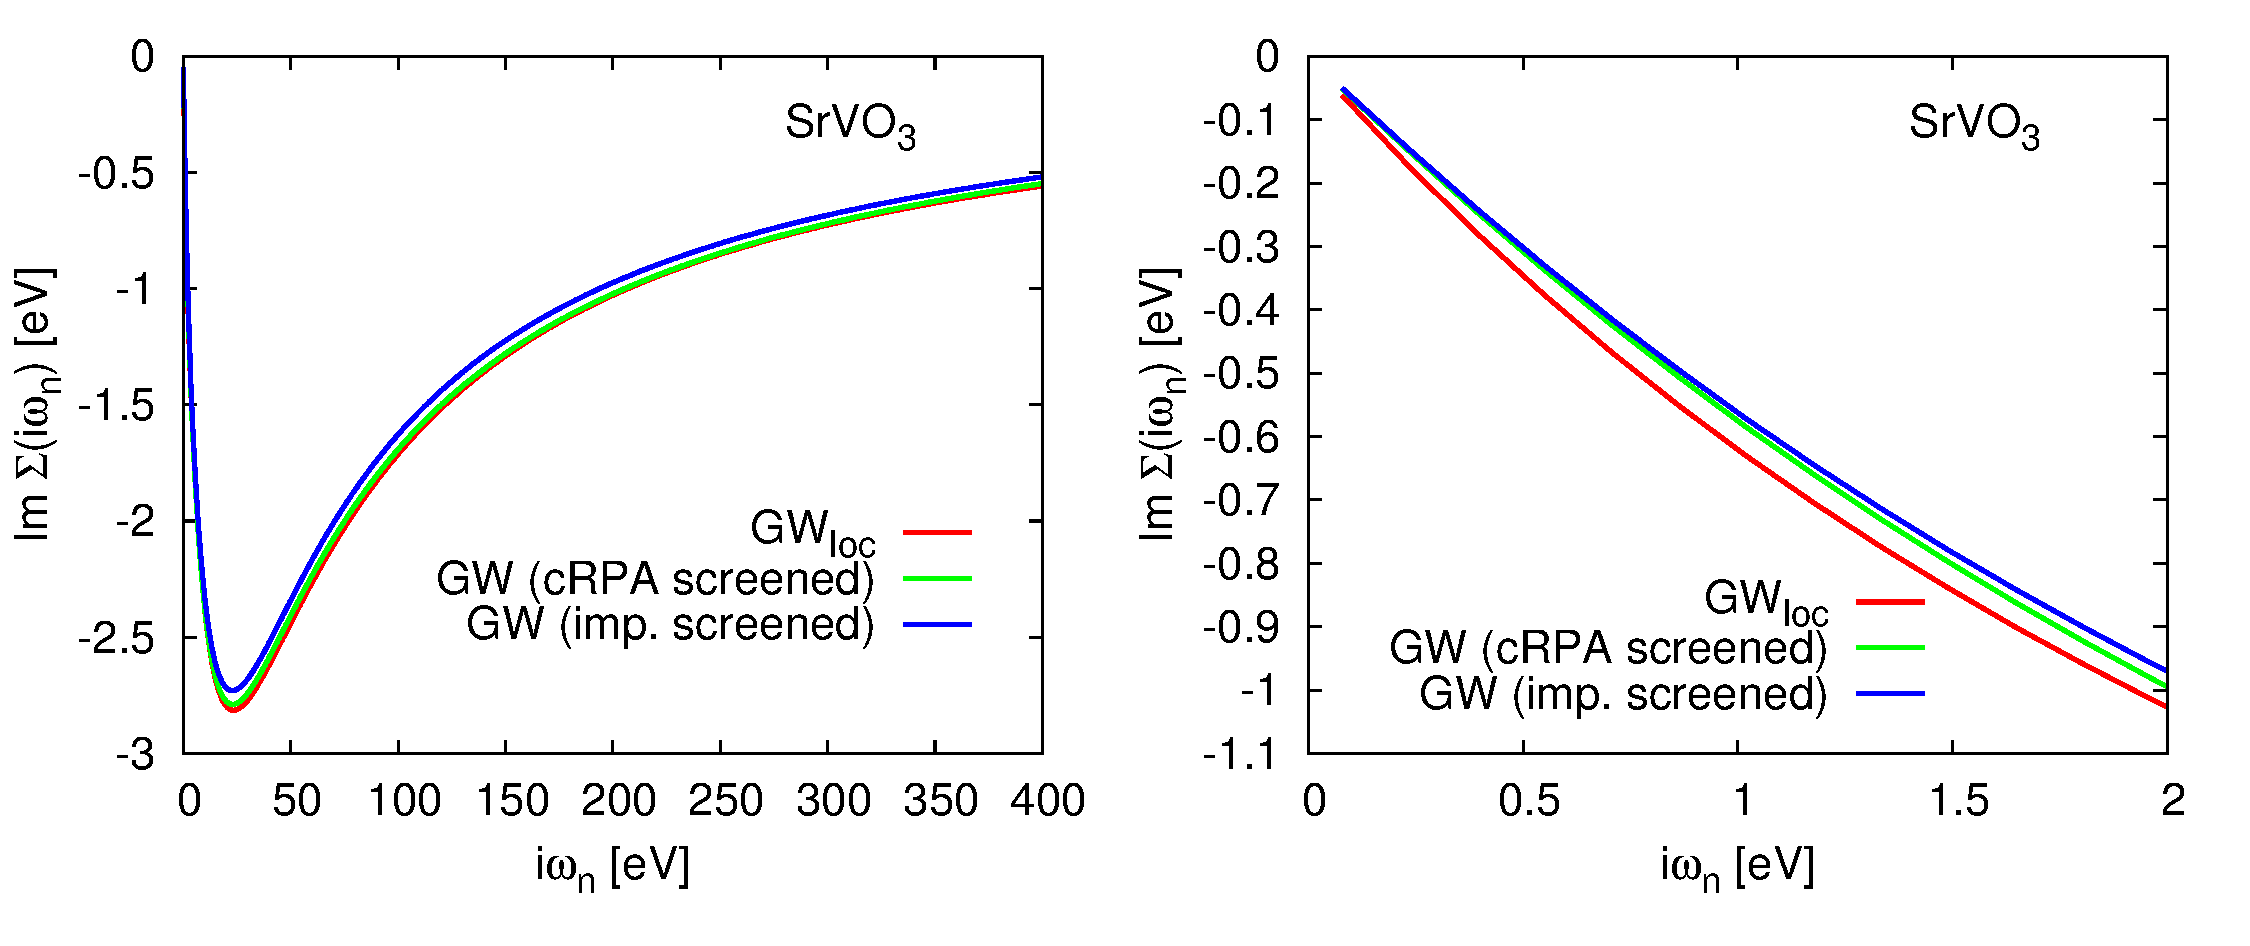
\includegraphics[width=1.0\textwidth]{figs/Wloc/Sigma_comp.pdf}
\caption{The local GW Selfenergy calculated as $\Sigma=G_{\mathrm{loc}}W_{\mathrm{loc}}$
using the different types of the screened interaction $W$ discussed
in Fig.~\ref{fig:W_loc_comparison}.
}
\label{fig:Sigma_GW_comparison}
\end{figure}

A comparison of the different Selfenergies $\Sigma=G_{\mathrm{loc}}W_{\mathrm{loc}}$
can be seen in Fig.~\ref{fig:Sigma_GW_comparison}.
Interestingly, we see that the Selfenergy calculated from the fully screened interaction 
$W$ directly in the GW code gives the most strongly correlated result.
The other two methods are less correlated but very similar, where
the approximation of $F_0$ screening only reduces the high-frequency value 
of $\Sigma$ slightly.
The difference between the first and the two latter might arise from
the fact that in the first the screened Hund's terms are smaller, which
leads to actually stronger corrlations in systems with only one
electron, as discussed elsewhere.
The resulting quasi-particle weights are $0.556$, $0.604$ and $0.609$.

%%%%%%%%%%%%%%%%%%%%%%%%%%%%%%%%%%%%%%%%%%%%%%%%%%%%%%%%%%%%%%%%%%%%%%%%%%
%%%%%%%%%%%%%%%%%%%%%%%%%%%%%%%%%%%%%%%%%%%%%%%%%%%%%%%%%%%%%%%%%%%%%%%%%%

\subsection{Possible problems with the DC}
One important factor is the causality of the different DC schemes.
The GW Selfenergy is causal and the impurity Selfenergy is causal,
but subtracting a DC term can make the combined Selfenergy noncausal
\begin{align}
\Sigma^{GW+DMFT} &= \Sigma^{GW,loc} - \Sigma^{DC} + \Sigma^{imp}.
\end{align}
It only comes down to personal preference, whether the DC should be understood
as taking out contibutions from GW, so that GW is a correction to DMFT
\begin{align}
\Sigma^{GW+DMFT} &=  \Sigma^{imp} + \left(\Sigma^{GW,loc} - \Sigma^{DC}\right) ,
\end{align}
or whether one takes out contibutions from DMFT, so that DMFT is a correction to GW
\begin{align}
\Sigma^{GW+DMFT} &=  \Sigma^{GW,loc} + \left(\Sigma^{imp} - \Sigma^{DC}\right) .
\end{align}
For now we do not seem to have this problem with the Doublecounting.

Noncausality appears in general in the hybridization function $\Delta$,
see Chapter~\ref{sec:noncausal_hyb}



%%%%%%%%%%%%%%%%%%%%%%%%%%%%%%%%%%%%%%%%%%%%%%%%%%%%%%%%%%%%%%%%%%%%%%%%%%
%%%%%%%%%%%%%%%%%%%%%%%%%%%%%%%%%%%%%%%%%%%%%%%%%%%%%%%%%%%%%%%%%%%%%%%%%%

\subsection{Evaluating the doublecounting factor $\Sigma^{DC}_{GW}=G_{loc}W_{loc}$}
\label{sec:glocwloc_dc_factor}
When evaluating the doublecounting factor 
\begin{align}
\Sigma^{DC}_{GW} &= -[G^{\mathrm{loc}}W^{\mathrm{loc}}],
\end{align}
we want to construct a Selfenergy which is solution
of the DMFT impurity problem within the GW approximation. 
By this, we regain exactly the full GW solution if we ``use GW
as the impurity solver''. In the GW+DMFT approach we use instead
DMFT as the impurity solver, which should give us corrections
that go beyond the GW approximation on the impurity.

Since we usually use the $G_0W_0$ approximation in the continuum,
for consistency we also have to solve the impurity problem within $G_0W_0$,
otherwise we would not regain the full $G_0W_0$ solution, as just discussed.
This means $G^{\mathrm{loc}}$ is the local DFT Green's function
in the correlated subspace and $W^{\mathrm{loc}}$ is the local 
\textit{effective} fully screened interaction on the impurity.
$W^{\mathrm{loc}}$ is just related to the effective ``bare'' interaction
that is the input for DMFT via the Dyson equation
\begin{align}
\mathcal{U}^{-1} &= [W^{loc} ]^{-1} + P^{imp}.
\end{align}
$W^{\mathrm{loc}}$ thus contains all the screening processes 
but is projected onto the correlated subspace.

To derive the expression for $G^{loc}W^{loc}$ we start with the definitions
from the original paper by Hedin (we set $\hbar=1$).
For real time in the continuum the Green's function and
the bare Coulomb potential is defined as (see Eq. (1) in Phys. Rev. 139, 3A (1965))
\begin{align}
G(1,2) &= -i \langle T \psi(1)\psi^{\dagger}(2) \rangle \\
V_C(1,2) &= \frac{\delta(t_1-t_2)}{|r_1-r_2|},
\end{align}
where the arguments denote the combined space,spin and time dependence
\begin{align}
 (1) &= (r_1,\sigma_1,t_1).
\end{align}
The Selfenergy in the GW approximation is then given as
(see Eq. (10) in Phys. Rev. 139, 3A (1965))
\begin{align}
 \Sigma(1,2) &= i G(1,2)W(1^+,2),
\end{align}
where
\begin{align}
 (1^+) &= (r_1,\sigma_1,t_1+\Delta), \hspace{0.5cm} \Delta\rightarrow 0^+.
\end{align}
It is instructive to investigate the case of no screening when 
$W$ is equal to the bare Coulomb potential
\begin{align}
 \Sigma(1,2) &= i G(1,2)W(1^+,2)                      \\
 &= i G(1,2) \frac{\delta(t_1+\Delta-t_2)}{|r_1-r_2|}  \\
 &= i G(r_1,\sigma_1,t_1;r_2,\sigma_2,t_1+\Delta) \frac{\delta(t_1+\Delta-t_2)}{|r_1-r_2|}  \\
 &= \langle T \psi_{\sigma_1}(r_1,t_1)\psi^{\dagger}_{\sigma_2}(r_2,t_1+\Delta) \rangle \frac{\delta(t_1+\Delta-t_2)}{|r_1-r_2|}  \\
 &= -\langle \psi^{\dagger}_{\sigma_2}(r_2)\psi_{\sigma_1}(r_1) \rangle \frac{\delta(t_1+\Delta-t_2)}{|r_1-r_2|}  \\
 %
\Rightarrow \Sigma(r_1,\sigma_1,t_1;r_2,\sigma_2,t_2)
&= -\frac{\langle \psi^{\dagger}_{\sigma_2}(r_2)\psi_{\sigma_1}(r_1) \rangle }{|r_1-r_2|}\delta(t_1-t_2) .
\end{align}
In this case the GW is just the bare Fock-exchange!
There is no Hartree contribution in the GW Selfenergy.
This means GW is basically just dynamically screened
exchange? Where do correlation terms come in?

Since we work on the Matsubara axis, we rewrite 
the equation for imaginary times
\begin{align}
G(1,2) &= - \langle T_{\tau} \psi(1)\psi^{\dagger}(2) \rangle \\
\Sigma(1,2) &= - G(1,2)W(1^+,2),
\end{align}
where the arguments now denote the imaginary time argument
\begin{align}
 (1) &= (r_1,\sigma_1,\tau_1) \\
 (1^+) &= (r_1,\sigma_1,\tau_1+\Delta).
\end{align}
For consistency we can check that setting $W$ equal
the bare Coulomb interaction indeed reduces to the
Fock-exchange with the correct sign. $GV_C$ is positive
but again exchaning the operators leads to an overall minus sign,
so the total contribution indeed is negative and identical
to the result on the real-time axis.

Introducing a local basis 
$\braket{r|\chi_{m}^{\sigma}}=\chi_{m}^{\sigma}(r)$ we can
obtain the matrix elements of the Selfenergy in this basis
\begin{align}
 \braket{m_1\sigma_1 | \Sigma(\tau_1,\tau_2) | m_2\sigma_2 } 
 &= \braket{\chi_{m_1}^{\sigma_1} | \Sigma(\tau_1,\tau_2) | \chi_{m_2}^{\sigma_2} }  \\
 &= -\int\int dr_1dr_2 \  \chi_{m_1}^{\sigma_1*}(r_1) G(r_1,\sigma_1,\tau_1;r_2,\sigma_2,\tau_2)\\
           & \hspace{3cm} \times W(r_1,\tau_1+\Delta;r_2,\tau_2)\chi_{m_2}^{\sigma_2}(r_2)
\end{align}
Expanding the Green's function in this local basis as
\begin{align}
 G(r_1,\sigma_1,\tau_1;r_2,\sigma_2,\tau_2)
 &= \sum_{kl} \chi_{k}^{\sigma_1}(r_1) G^{\sigma_1\sigma_2}_{kl}(\tau_1,\tau_2)\chi_{l}^{\sigma_2*}(r_2)
\end{align}
we get
\begin{align}
 \braket{m_1\sigma_1 | \Sigma(\tau_1,\tau_2) | m_2\sigma_2 } 
 &= -\sum_{kl}\int\int dr_1dr_2 \  G^{\sigma_1\sigma_2}_{kl}(\tau_1,\tau_2)\\
           & \hspace{0cm} \times \chi_{m_1}^{\sigma_1*}(r_1)\chi_{l}^{\sigma_2*}(r_2) W(r_1,\tau_1+\Delta;r_2,\tau_2) \chi_{k}^{\sigma_1}(r_1) \chi_{m_2}^{\sigma_2}(r_2)
\end{align}
The last term we identify as the matrix element of the fully
screened interaction
\begin{align}
 \braket{m_1 l | W(\tau_1+\Delta,\tau_2) | k m_2} 
 &=\int\int dr_1dr_2  \chi_{m_1}^{\sigma_1*}(r_1)\chi_{l}^{\sigma_2*}(r_2) W(r_1,\tau_1+\Delta;r_2,\tau_2) \chi_{k}^{\sigma_1}(r_1) \chi_{m_2}^{\sigma_2}(r_2)
\end{align}
With this we finally get the expression
\begin{align}
 \braket{m_1\sigma_1 | \Sigma(\tau_1,\tau_2) | m_2\sigma_2 } 
 &= -\sum_{kl} \braket{m_1 l | W(\tau_1+\Delta,\tau_2) | k m_2}G^{\sigma_1\sigma_2}_{kl}(\tau_1,\tau_2)
\end{align}
We can simplify this expression by assuming time translational
invariance and assume the local Green's function to
be orbital- and spin-diagonal
\begin{align}
  \Sigma_m^{\sigma}(\tau) 
 &= -\sum_{k} \braket{m k | W(\tau+\Delta)|k m} G^{\sigma}_{k}(\tau)
\end{align}
Again we see that the GW Selfenergy is basically dynamical
screened exchange. 

Applying the Fourier transform and inserting the 
Fourier transform of $G(ix_n)$ and $W(i\nu_n)$ we get for the
Selfenergy on the Matsubara axis
\begin{align}
  \Sigma_m^{\sigma}(i\omega_n) 
  &= -\sum_k\int_{0}^{\beta}d\tau \ 
  \left[\frac{1}{\beta}\sum_i \braket{m k | W(i\nu_i)|k m} \mathrm{e}^{-i\nu_i(\tau+\Delta)} \right]
  \left[\frac{1}{\beta}\sum_j G^{\sigma}_{k}(ix_j) \mathrm{e}^{-i\nu_i\tau} \right]
  \mathrm{e}^{i\omega_n\tau} \\
  %
  &= -\sum_k \sum_{ij} \braket{m k | W(i\nu_i)|k m}G^{\sigma}_{k}(ix_j)
    \int_{0}^{\beta}d\tau \ 
  \frac{1}{\beta^2}  \mathrm{e}^{i(\omega_n -\nu_i -x_j)\tau}
   \mathrm{e}^{-i\nu_i \Delta} \\
   %
   &= -\frac{1}{\beta}\sum_k \sum_{j}
   \braket{m k | W(i\nu_j)|k m}G^{\sigma}_{k}(i\omega_n-i\nu_j)
   \mathrm{e}^{-i\nu_j \Delta}
\end{align}
(This form should not be used, see below)
Or rewriting the frequency sum we get the alternative version
\begin{align}
  \Sigma_m^{\sigma}(i\omega_n) 
   &= -\frac{1}{\beta}\sum_k \sum_{j}
   \braket{m k | W(i\omega_n- ix_j )|k m}G^{\sigma}_{k}(ix_j)
   \mathrm{e}^{-i(\omega_n- x_j )\Delta} \\
   &= -\frac{1}{\beta}\sum_k \sum_{j}
   \braket{m k | W(i\omega_n- ix_j )|k m}G^{\sigma}_{k}(ix_j)
   \mathrm{e}^{ix_j \Delta}
\end{align}
The last factor $\mathrm{e}^{ix_j \Delta}$ is important
to ensure convergence of the frequency sum. 
This form is actually much better for practical implementation because
the slow $1/i\omega_j$ convergence does not include a shift which
slows down the convergence even more. 
Since $\Delta\rightarrow 0^+$ we can directly see
that we regain the correct Fock-exchange when replacing
$W$ by the constant bare Coulomb interaction!
For the GW solution of the impurity model 
the sum over the orbital indices $k$ is performed
only over the correlated subspace which spans
the Hilbert space of the Anderson impurity model.


It is instructive to look at the case of a simple
degenerate $t_{2g}$-only model like for SrVO$_3$. In this case
we define the screened on-site Coulomb matrix element and the 
screened Hund's exchange as
\begin{align}
 \braket{k k | W(i\nu )|k k} &= U_0(i\nu) \\
 \braket{m k | W(i\nu )|k m} &= J(i\nu), \ \ \ k\neq m.
\end{align}
With this we get the explicit expression for
the $t_{2g}$ Selfenergy
\begin{align}
  \Sigma^{\sigma}(i\omega_n) 
   &= -\frac{1}{\beta}\sum_{ix_j}
   \Big( U_0(i\omega_n- ix_j )  + 2 J(i\omega_n- ix_j ) \Big)G^{\sigma}(ix_j)
   \mathrm{e}^{ix_j \Delta}
\end{align}
The first term corresponding to 
$U_0$ is similar to a dynamical self-interaction correction since it 
originates from an interaction with a state with the
same orbital and spin index.
The second term corresponding to $J$ is a dynamical
intraatomic exchange contribution
since it 
originates from an interaction with a state in a different
orbital and with the same spin index.

Again we see that the GW Selfenergy has the characteristics
of a dynamically screened Fock-exchange term. 
% Still, it is responsible for a finite renormalization
% larger than 1, i.e. it still reduces the Bandwidth!
% This can be seen from the slope of the Selfenergy
%  \begin{align}
%  \lim_{i\omega_n\rightarrow 0} &
%  \frac{\partial}{\partial i\omega_n}
%   \Sigma^{\sigma}(i\omega_n)  \\
%   %
%    &= -\frac{1}{\beta}\sum_k \sum_{j}
%    \braket{m k | W(i\nu_j)|k m }
%    \mathrm{e}^{-i\nu_j \Delta}
%       \left[ 
%    \lim_{i\omega_n\rightarrow 0}  \frac{\partial}{\partial i\omega_n}G^{\sigma}_{k}(i\omega_n-i\nu_j) \right]
%   %
%   &= -\frac{1}{\beta}\sum_k \sum_{j}
%   \braket{m k | W(i\nu_j)|k m }
%   \mathrm{e}^{-i\nu_j \Delta}
%     \left[ 
%   \lim_{i\omega_n\rightarrow 0}  \frac{\partial}{\partial i\omega_n}G^{\sigma}_{k}(i\omega_n-i\nu_j) \right]   
% \end{align}

%%%%%%%%%%%%%%%%%%%%%%%%%%%%%%%%%%%%%%%%%%%%%%%%%%%%%%%%%%%%%%%%%%%%%%%%%%
%%%%%%%%%%%%%%%%%%%%%%%%%%%%%%%%%%%%%%%%%%%%%%%%%%%%%%%%%%%%%%%%%%%%%%%%%%

\subsection{High-frequency correction for GW-DC version1}
\cng{This should not be used because this form converges slower}
When evaluating the frequency sum for the doublecounting in the form 
\begin{align}
  \Sigma_m^{\sigma}(i\omega_n) 
%
  &= -\frac{1}{\beta}\sum_k \sum_{j}
   \braket{m k | W(i\nu_j)|k m}G^{\sigma}_{k}(i\omega_n-i\nu_j)
   \mathrm{e}^{-i\nu_j \Delta}
\end{align}
the convergence is not so good and needs to be corrected
for the high-frequency parts.
We use a high-frequency form to fit the Green's function and interaction
given by
\begin{align}
 W(i\nu_n)    &\approx w_0 + \frac{w_2}{(i\nu_n)^2} \ \in \mathbb{R} \\
 G(i\omega_n) &\approx  \frac{1}{i\omega_n} + \frac{g_2}{(i\omega_n)^2} 
\end{align}
We need to evaluate the following high-frequency terms (orbital/spin etc indices
are suppressed)
\begin{align}
& -\frac{1}{\beta}\sum_{j\neq 0} 
  \left( w_0 + \frac{w_2}{(i\nu_j)^2} \right)
  \left( \frac{1}{i\omega_n-i\nu_j} + \frac{g_2}{(i\omega_n-i\nu_j)^2} \right)
   \mathrm{e}^{-i\nu_j \Delta} \\
% 
&= -\frac{1}{\beta} \sum_{j\neq 0}
\left( 
  \frac{w_0}{i\omega_n-i\nu_j} + \frac{w_0 g_2}{(i\omega_n-i\nu_j)^2}
+ \frac{w_2}{(i\nu_j)^2(i\omega_n-i\nu_j)} + \frac{w_2g_2}{(i\nu_j)^2(i\omega_n-i\nu_j)^2}
\right)
\mathrm{e}^{-i\nu_j \Delta}.
\end{align}
Evaluating the terms analytically we get for the first term (compare Steffen's PhD thesis
for the derivation)
\begin{align}
   -\frac{1}{\beta}\sum_{j\neq 0} \frac{w_0}{i\omega_n-i\nu_j}\mathrm{e}^{-i\nu_j \Delta}
&= -\frac{w_0}{\beta}\left(-\frac{1}{i\omega_n-0}\mathrm{e}^{-i0 \Delta} + \sum_{j} \frac{1}{i\omega'_j}\mathrm{e}^{-(i\omega_n-i\omega'_j) \Delta}\right) \\
&= -\frac{w_0}{\beta}\left( -\frac{1}{i\omega_n}
       +\mathrm{e}^{-i\omega_n \Delta} \sum_{j\neq 0} \frac{1}{i\omega'_j}\mathrm{e}^{i\omega'_j \Delta} \right) \\
&= -\frac{w_0}{\beta}
       \left(-\frac{1}{i\omega_n} +  \frac{\beta}{2}\right) \\
&= w_0 \left( \frac{1}{i(2n+1)\pi} - \frac{1}{2} \right) .
\end{align}
The second term
\begin{align}
   -\frac{1}{\beta}\sum_{j\neq 0} \frac{w_0 g_2}{(i\omega_n-i\nu_j)^2}\mathrm{e}^{-i\nu_j \Delta}
&= -\frac{w_0 g_2}{\beta}\sum_{j\neq 0} \frac{1}{(i\omega'_j)^2}\mathrm{e}^{-(i\omega_n-i\omega'_j) \Delta} \\
&= -\frac{w_0 g_2}{\beta} \mathrm{e}^{-i\omega_n\Delta} \sum_{j\neq 0} \frac{1}{(i\omega'_j)^2}\mathrm{e}^{i\omega'_j \Delta} \\
&= -\frac{w_0 g_2}{\beta} \mathrm{e}^{-i\omega_n\Delta}
     \left(-\frac{1}{(i\omega'_{j=0})^2}\mathrm{e}^{i\omega'_{j=0} \Delta} +  \sum_{j} \frac{1}{(i\omega'_j)^2}\mathrm{e}^{i\omega'_j \Delta} \right) \\
&= -\frac{w_0 g_2}{\beta} \mathrm{e}^{-i\omega_n\Delta}
      \left(\frac{\beta^2}{\pi^2} +  \frac{-2\Delta - \beta}{4}\beta \right) \\
&= w_0 g_2\beta \left( \frac{1}{4} - \frac{1}{\pi^2} \right).
\end{align}
The third term
\begin{align}
-\frac{1}{\beta}\sum_{j\neq 0} & \frac{w_2}{(i\nu_j)^2(i\omega_n-i\nu_j)}\mathrm{e}^{-i\nu_j \Delta} \\
&= -\frac{iw_2\beta^2}{(8n- 4)\pi^3}\left( \frac{2n-1}{2n+1}\frac{\pi^2}{6} \right)
   -\frac{iw_2\beta^2}{(8n+12)\pi^3}\left( \frac{2n+3}{2n+1}\frac{\pi^2}{6} -\frac{8n+12}{(2n+1)^3}\right) \\
&= -\frac{iw_2\beta^2}{\pi^3}\left( \frac{\pi^2}{12(2n+1)} - \frac{1}{(2n+1)^3} \right)   \\
&= -\frac{iw_2\beta^2}{(2n+1)\pi^3}\left( \frac{\pi^2}{12} - \frac{1}{(2n+1)^2} \right) .
\end{align}
The fourth term
\begin{align}
 -\frac{1}{\beta}\sum_{j\neq 0} & \frac{w_2g_2}{(i\nu_j)^2(i\omega_n-i\nu_j)^2} \mathrm{e}^{-i\nu_j \Delta} \\
&= -\frac{w_2g_2\beta^3}{4\pi^4(2n-1)^2}\left( \frac{(2n-1)^2}{(2n+1)^2}\frac{\pi^2}{6} \right)
   -\frac{w_2g_2\beta^3}{4\pi^4(2n+3)^2}\left( \frac{(2n+3)^2}{(2n+1)^2}\frac{\pi^2}{6} -12\frac{(2n+3)^2}{(2n+1)^4}\right) \\
%
&= -\frac{w_2g_2\beta^3}{4\pi^4}\left(  \frac{\pi^2}{3(2n+1)^2}  -\frac{12}{(2n+1)^4} \right) \\
&= -\frac{w_2g_2\beta^3}{\pi^4(2n+1)^2}\left(  \frac{\pi^2}{12}  -\frac{3}{(2n+1)^2} \right) .
\end{align}


\subsection{High-frequency correction for GW-DC version2}
When evaluating the frequency sum for the doublecounting in the form 
\begin{align}
  \Sigma_m^{\sigma}(i\omega_n) 
%
  &= -\frac{1}{\beta}\sum_k \sum_{j}
   \braket{m k | W(i\omega_n- ix_j )|k m}G^{\sigma}_{k}(ix_j)
   \mathrm{e}^{ix_j \Delta}
\end{align}
the convergence is quite fast but still needs to be corrected
for the high-frequency parts.
We use a high-frequency form to fit the Green's function and interaction
given by
\begin{align}
 W(i\nu_n)    &\approx w_0 + \frac{w_1}{i\nu_n} + \frac{w_2}{(i\nu_n)^2}  \\
 G(i\omega_n) &\approx  \frac{1}{i\omega_n} + \frac{g_2}{(i\omega_n)^2} 
\end{align}
The screened interactin $W$ on the Matsubara axis can in general be complex
and thus has a term $\sim 1/i\nu_n$ for non-degenerate orbitals 
due to the local projection (as discussed with Ferdi).
We need to evaluate the following high-frequency terms (orbital/spin etc indices
are suppressed, and the $j=n$ term is taken out because
the form of $W$ diverges at this point)
\begin{align}
& -\frac{1}{\beta}\sum_{j\neq n} 
  \left( w_0 + \frac{w_1}{i\omega_n -ix_j} + \frac{w_2}{(i\omega_n -ix_j)^2} \right)
  \left( \frac{1}{ix_j} + \frac{g_2}{(ix_j)^2} \right)
   \mathrm{e}^{ix_j \Delta} \\
% 
&= -\frac{1}{\beta} \sum_{j\neq n}
\left( 
  \frac{w_0}{ix_j} + \frac{w_0 g_2}{(ix_j)^2}
+ \frac{w_1}{ix_j(i\omega_n -ix_j)} + \frac{w_1g_2}{(ix_j)^2(i\omega_n -ix_j)}  \right.\nonumber\\
&\hspace{2.5cm}+ \left.\frac{w_2}{ix_j(i\omega_n -ix_j)^2} + \frac{w_2g_2}{(ix_j)^2 (i\omega_n -ix_j)^2}
\right)
\mathrm{e}^{ix_j \Delta}.
\end{align}
Evaluating the terms analytically we get for the first term (compare Steffen's PhD thesis
for the derivation)
\begin{align}
-\frac{1}{\beta} \sum_{j\neq n}  \frac{w_0}{ix_j} \mathrm{e}^{ix_j \Delta}
&= -\frac{w_0}{\beta} \left( -\frac{1}{ix_n} \mathrm{e}^{ix_n \Delta}  + \sum_{j}  \frac{1}{ix_j} \mathrm{e}^{ix_j \Delta}\right) \\
&= w_0 \left( \frac{1}{i(2n+1)\pi} -\frac{1}{2} \right).
\end{align}
The second term
\begin{align}
-\frac{1}{\beta} \sum_{j\neq n}  \frac{w_0 g_2}{(ix_j)^2} \mathrm{e}^{ix_j \Delta} 
&= -\frac{w_0 g_2}{\beta}\left(- \frac{1}{(ix_n)^2} \mathrm{e}^{ix_n \Delta}   + \sum_{j}  \frac{1}{(ix_j)^2} \mathrm{e}^{ix_j \Delta}\right)   \\
&= -w_0 g_2\left( \frac{\beta}{(2n+1)^2\pi^2} + \frac{-2\Delta-\beta}{4} \right)   \\
&=  w_0 g_2\beta\left( \frac{1}{4} -\frac{1}{(2n+1)^2\pi^2} \right) .
\end{align}
The third term
(we set the exponential term directly to zero since these sums converge, so the limit and sum can be
swapped)
\begin{align}
-\frac{1}{\beta} \sum_{j\neq n}  \frac{w_1}{i\omega_n-i\nu_j} \frac{1}{ix_j} 
&= \frac{w_1}{\beta} \sum_{j\neq n}  \frac{1}{2(n-j)\frac{\pi}{\beta} (2j+1)\frac{\pi}{\beta}} \\
&= \frac{w_1\beta}{2\pi^2} \sum_{j\neq n}  \frac{1}{(n-j)(2j+1)} \\
&= -\frac{ w_1 \beta }{(2n+1)^2 \pi^2} ,
\end{align}
The fourth term becomes
\begin{align}
-\frac{1}{\beta} \sum_{j\neq n}  \frac{w_1}{i\omega_n-i\nu_j} \frac{g_2}{(ix_j)^2} 
&= -i\frac{w_1g_2}{\beta} \sum_{j\neq n}  \frac{1}{2(n-j)\frac{\pi}{\beta} (2j+1)^2\frac{\pi^2}{\beta^2}} \\
&= -i\frac{w_1 g_2 \beta^2}{2\pi^3} \sum_{j\neq n}  \frac{1}{(n-j)(2j+1)^2} \\
&= -i\frac{w_1 g_2 \beta^2}{(2n+1)^3 \pi} \left( n^2 + n + \frac{1}{4} - \frac{2}{\pi^2} \right).
\end{align}
The fifth term (using Maple software)
\begin{align}
-\frac{1}{\beta} \sum_{j\neq n}  \frac{w_2}{ix_j(i\omega_n -ix_j)^2} \mathrm{e}^{ix_j \Delta} 
&= i\frac{w_2\beta^2}{\pi^3}\left( \frac{1}{(2n+1)^3} - \frac{\pi^2}{12(2n+1)} \right) \\
&= i\frac{w_2\beta^2}{(2n+1)\pi^3}\left( \frac{1}{(2n+1)^2} - \frac{\pi^2}{12} \right) 
\end{align}
The sixth term (using Maple software)
\begin{align}
-\frac{1}{\beta} \sum_{j\neq n}  \frac{w_2g_2}{(ix_j)^2 (i\omega_n -ix_j)^2} \mathrm{e}^{ix_j \Delta} 
&= \frac{w_2g_2\beta^3}{4\pi^4}\left( \frac{12}{(2n+1)^4} - \frac{\pi^2}{3(2n+1)^2} - \frac{\pi^2}{(2n+1)^2} \right) \\
&= \frac{w_2g_2\beta^3}{(2n+1)^2\pi^4}\left( \frac{3}{(2n+1)^2} - \frac{\pi^2}{3} \right).
\end{align}

With this, the final expression implemented in the Code is then given by
\begin{align}
  \Sigma_m^{\sigma}(i\omega_n) 
%
  =& \sum_k\Bigg[ -\frac{1}{\beta} 
   \braket{m k | W(0 )|k m}G^{\sigma}_{k}(i\omega_n) \nonumber \\
%
   & \hspace{2cm}-\frac{1}{\beta}\sum_{j\neq n}^{\pm N_{max}} 
   \Big[ \braket{m k | W(i\omega_n- ix_j ) |k m}  G^{\sigma}_{k}(ix_j) \nonumber \\
%
   &\hspace{3.8cm} -\left( w^{mk}_0 + \frac{w^{mk}_1}{i\omega_n -ix_j} + \frac{w^{mk}_2}{(i\omega_n- ix_j)^2}\right)
       \left( \frac{1}{ix_j} + \frac{g^k_2}{(ix_j)^2} \right)  \Big]\nonumber \\
   %
& +w^{mk}_0 \left( \frac{1}{i(2n+1)\pi} -\frac{1}{2} \right) 
  + w^{mk}_0 g^k_2\beta\left( \frac{1}{4} -\frac{1}{(2n+1)^2\pi^2} \right) \nonumber \\
%
& -\frac{ w^{mk}_1 \beta }{(2n+1)^2 \pi^2} 
  -i\frac{w^{mk}_1 g^k_2 \beta^2}{(2n+1)^3 \pi} \left( n^2 + n + \frac{1}{4} - \frac{2}{\pi^2} \right)\nonumber \\
%
& + i\frac{w^{mk}_2\beta^2}{(2n+1)\pi^3}\left( \frac{1}{(2n+1)^2} - \frac{\pi^2}{12} \right) 
  + \frac{w^{mk}_2g^k_2\beta^3}{(2n+1)^2\pi^4}\left( \frac{3}{(2n+1)^2} - \frac{\pi^2}{3} \right) \Bigg] .
 \end{align}
 
%%%%%%%%%%%%%%%%%%%%%%%%%%%%%%%%%%%%%%%%%%%%%%%%%%%%%%%%%%%%%%%%%%%%%%%%%%%%%%%%%%%%% 
%%%%%%%%%%%%%%%%%%%%%%%%%%%%%%%%%%%%%%%%%%%%%%%%%%%%%%%%%%%%%%%%%%%%%%%%%%%%%%%%%%%%%
 
\subsection{High-frequency correction for $P=G_{loc}G_{loc}$}
For the local polarization used for the doublecounting we have to evaluate
the expression (see chapter~\ref{sec:local_w_p_matsubara})
\begin{align}
 P^{\sigma\sigma'}_{ijkl}(i\nu_n)
%
 &=\frac{1}{\beta} \sum_{i\omega_n} G^{\sigma\sigma'}_{ij}(i\omega_n)
                     G^{\sigma'\sigma}_{lk}(i\omega_n-i\nu_n) \mathrm{e}^{i\omega_n\Delta},
\end{align}
with $\Delta \rightarrow 0^+$.
For the high-frequency correction we expand the Green's function
at large frequencies as
\begin{align}
 G^{\sigma\sigma'}_{ij}(i\omega_n)
 &\approx \frac{1}{i\omega_n} + \frac{c^{\sigma\sigma'}_{ij}}{(i\omega_n)^2}.
\end{align}
This leads to the following corrected summation
\begin{align}
 P^{\sigma\sigma'}_{ijkl}(i\nu_n)
%
 &=\frac{1}{\beta} \sum_{n=-N}^{N}\left[ G^{\sigma\sigma'}_{ij}(i\omega_n)
                                   G^{\sigma'\sigma}_{lk}(i\omega_n-i\nu_n)
           -\left( \frac{1}{i\omega_n} + \frac{g^{\sigma\sigma'}_{ij}}{(i\omega_n)^2}\right)
            \left(\frac{1}{i\omega_n-i\nu_n} + \frac{g^{\sigma'\sigma}_{lk}}{(i\omega_n-i\nu_n)^2}\right)\right] \nonumber \\
%
&\hspace{0.5cm}+ \frac{1}{\beta} \sum_{i\omega_n} 
            \left( \frac{1}{i\omega_n} + \frac{g^{\sigma\sigma'}_{ij}}{(i\omega_n)^2}\right)
            \left( \frac{1}{i\omega_n-i\nu_n} + \frac{g^{\sigma'\sigma}_{lk}}{(i\omega_n-i\nu_n)^2}\right)
             \mathrm{e}^{i\omega_n\Delta}.
\end{align}
The second term can be evaluated analytically with the following contributions:
The first term is
\begin{align}
\frac{1}{\beta} \sum_{i\omega} \frac{1}{i\omega_n}\frac{1}{i\omega_n-i\nu_n} \mathrm{e}^{i\omega_n\Delta}
&= \begin{cases}
    - \beta / 4 & \mbox{ for } n=0 \\
     0 & \mbox{ else}
   \end{cases}.
\end{align}

The second term is
\begin{align}
\frac{1}{\beta} \sum_{i\omega} \frac{1}{i\omega_n}\frac{g^{\sigma'\sigma}_{lk}}{(i\omega_n-i\nu_n)^2} \mathrm{e}^{i\omega_n\Delta}
&= \begin{cases}
    0 & \mbox{ for } n=0 \\
    i \beta^2 g^{\sigma'\sigma}_{lk} / 8n\pi & \mbox{ else}
   \end{cases}.
\end{align}
The third term is
\begin{align}
\frac{1}{\beta} \sum_{i\omega} \frac{g^{\sigma\sigma'}_{ij}}{(i\omega_n)^2}\frac{1}{i\omega_n-i\nu_n} \mathrm{e}^{i\omega_n\Delta}
&= \begin{cases}
    0 & \mbox{ for } n=0 \\
    -i \beta^2 g^{\sigma\sigma'}_{ij} / 8n\pi & \mbox{ else}
   \end{cases}.
\end{align}

The last and fourth term is
\begin{align}
\frac{1}{\beta} \sum_{i\omega} \frac{g^{\sigma\sigma'}_{ij}}{(i\omega_n)^2}\frac{g^{\sigma'\sigma}_{lk}}{(i\omega_n-i\nu_n)^2} \mathrm{e}^{i\omega_n\Delta}
&= \begin{cases}
    \beta^3 g^{\sigma\sigma'}_{ij}g^{\sigma'\sigma}_{lk}/48 & \mbox{ for } n=0 \\
    \beta^3 g^{\sigma\sigma'}_{ij}g^{\sigma'\sigma}_{lk}/8n^2\pi^2 & \mbox{ else}
   \end{cases}.
\end{align}

The full expression thus reads
\begin{align}
 P^{\sigma\sigma'}_{ijkl}(i\nu_n)
%
 &=\frac{1}{\beta} \sum_{n=-N}^{N}\left[ G^{\sigma\sigma'}_{ij}(i\omega_n)
                                   G^{\sigma'\sigma}_{lk}(i\omega_n-i\nu_n)
           -\left( \frac{1}{i\omega_n} + \frac{g^{\sigma\sigma'}_{ij}}{(i\omega_n)^2}\right)
            \left(\frac{1}{i\omega_n-i\nu_n} + \frac{g^{\sigma'\sigma}_{lk}}{(i\omega_n-i\nu_n)^2}\right)\right] \nonumber \\
%
&\hspace{0.5cm}+ 
\begin{cases}
  (\beta^3 g^{\sigma\sigma'}_{ij}g^{\sigma'\sigma}_{lk} - 12\beta)/48 & \mbox{ for } n=0 \\
  \beta^3 g^{\sigma\sigma'}_{ij}g^{\sigma'\sigma}_{lk}/8n^2\pi^2
  + i \beta^2 (g^{\sigma'\sigma}_{lk}-g^{\sigma\sigma'}_{ij}) / 8n\pi & \mbox{ else} 
\end{cases}.
\end{align}

Assuming the local Green's function is diagonal in orbital and spin-indices,
we get the following expression
\begin{align}
 P^{\sigma}_{iikk}(i\nu_n)
%
 &=\frac{1}{\beta} \sum_{n=-N}^{N}\left[ G^{\sigma}_{i}(i\omega_n)
                                   G^{\sigma}_{k}(i\omega_n-i\nu_n)
           -\left( \frac{1}{i\omega_n} + \frac{g^{\sigma}_{i}}{(i\omega_n)^2}\right)
            \left(\frac{1}{i\omega_n-i\nu_n} + \frac{g^{\sigma}_{k}}{(i\omega_n-i\nu_n)^2}\right)\right] \nonumber \\
%
&\hspace{0.5cm}+ 
\begin{cases}
  (\beta^3 g^{\sigma}_{i}g^{\sigma}_{k} - 12\beta)/48 & \mbox{ for } n=0 \\
  \beta^3 g^{\sigma}_{i}g^{\sigma}_{k}/8n^2\pi^2
  + i \beta^2 (g^{\sigma}_{k}-g^{\sigma}_{i}) / 8n\pi & \mbox{ else} 
\end{cases}.
\end{align}


%%%%%%%%%%%%%%%%%%%%%%%%%%%%%%%%%%%%%%%%%%%%%%%%%%%%%%%%%%%%%%%%%%%%%%%%%%%%%%%%%%%%%
%%%%%%%%%%%%%%%%%%%%%%%%%%%%%%%%%%%%%%%%%%%%%%%%%%%%%%%%%%%%%%%%%%%%%%%%%%%%%%%%%%%%%
%%%%%%%%%%%%%%%%%%%%%%%%%%%%%%%%%%%%%%%%%%%%%%%%%%%%%%%%%%%%%%%%%%%%%%%%%%%%%%%%%%%%%
%%%%%%%%%%%%%%%%%%%%%%%%%%%%%%%%%%%%%%%%%%%%%%%%%%%%%%%%%%%%%%%%%%%%%%%%%%%%%%%%%%%%%
%%%%%%%%%%%%%%%%%%%%%%%%%%%%%%%%%%%%%%%%%%%%%%%%%%%%%%%%%%%%%%%%%%%%%%%%%%%%%%%%%%%%%

 
\subsection{Doublecounting of the Hartree Term}
In the GW+DMFT cycle we have to deal with two types of doublecounting
when adding the GW and the DMFT Selfenergy to the Green's function, as
partially discussed before
\begin{align}
 G(k,i\omega_n) 
 &= \left[ \unity(i\omega_n+\mu ) -H^{DFT}(k) + v^{XC}(k) + \Sigma^{Hartree}_{DFT} \right.\nonumber\\
          & \hspace{1cm}- \Sigma^{XC}_{GW}(k,i\omega_n) 
          + \Sigma_{GW}^{DC}(i\omega_n)
          \left. - \Sigma_{imp}(i\omega_n)
           \right]^{-1},
\end{align}
The first one is the doublecounting of the Hartree term, which arises since it is
taken into account in the DFT and in the DMFT energies resp. Selfenergy.
Since DMFT can induce a charge transfer, we will subtract the initial DFT Hartree
contribution from the DFT energies, and add the full DMFT Selfenergy
which contains a selfconsistent Hartree calculated from the 
new orbital occupations. This Hartree correction is the Hartree term of the impurity,
i.e. it is only calculated from the correlated orbitals.
If the DFT charge is close to the exact charge, this term 
will be quite good, but if not DMFT can introduce a correction to that.

The second one is the local part of the Selfenergy, which
is contained in both the GW and the DMFT Selfenergy. Since we assume that DMFT
does a better job for the local Selfenergy, we subtract this part from the
GW Selfenergy and replace it by the local DMFT Selfenergy. 
The form of the Hartree part will be derived in section \ref{sec:hartree_exchange}.
If there is no charge transfer, the
Hartree part in the DMFT impurity Selfenergy is identical to the 
DFT Hartree part, so what has to be subtracted is a Hartree Selfenergy
given by the DFT fillings.
The fillings are calculated from the DFT Green's function, so
in the same sense as the GW doublecounting, we calculate the Hartree solution
of the impurity model, and subtract it as a doublecounting.
Therefore, it depends on the local DFT Green's function 
and the effective screened interaction $U(\omega)$. 

As derived above in section \ref{sec:glocwloc_dc_factor},
the GW doublecounting $\Sigma_{GW}^{DC}$ does not contain the Hartree but only the exchange part,
regardless whether it is calculated as $G_{loc}W_{loc}$ or $[GW]_{loc}$.
Therefore, there is no doublecounting of any Hartree term.

\bigskip

We do not need to worry about any exchange doublecounting because in
\begin{align}
 H^{DFT}(k) - v^{XC}(k)
\end{align}
there is only the Hartree contribution left. In the full
combination of 
\begin{align}
 \underbrace{H^{DFT}(k) - v^{XC}(k) - \Sigma^{Hartree}_{DFT}}_{\mbox{no exchange/no Hartree}}
          + \underbrace{\Sigma^{XC}_{GW}(k,i\omega_n) - \Sigma_{GW}^{DC}(i\omega_n)}_{\mbox{only nonlocal exch.}}
          + \underbrace{\Sigma_{imp}(i\omega_n)}_{\mbox{only local exch./Hartree}}
\end{align}
we can see that all DFT exchange is first replaced by the improved GW exchange.
The due to the GW Doublecounting the local exchange of the correlated subspace
is subtracted, and then again the local impurity exchange is added.

There is still some local exchange in the term 
$\Sigma^{XC}_{GW}(k,i\omega_n) - \Sigma_{GW}^{DC}(i\omega_n)$ but it is originating
from outside the correlated subspace or from couplings between the subspace and the remaining
space, which is not contained in $\Sigma_{imp}(i\omega_n)$.

The GW doublecounting approaches the local Fock part in the large $i\omega_n$ limit,
which means that we simply get the unscreened Fock-exchange 
values (compare with Section \ref{sec:glocwloc_dc_factor})
\begin{align}
\lim_{i\omega_n\rightarrow \infty} \Sigma^{DC}_{GW,L}(i\omega_n) 
&= -\frac{1}{\beta} \sum_{i\nu_n}\sum_{L'} G_{loc,L'}(i\omega_n-i\nu_n)V_{loc,LL'LL'} \\
&= - \sum_{L'} n_LV_{loc,LL'LL'} .
\end{align}


When performing a pure DMFT calculation where no GW Selfenergy is added,
we do not subtract the exchange correlation potential $V_{XC}$.
Then we should subtract the full local Hartree \textbf{and} Fock exchange terms.
By this, the local Hartree and Fock exchange terms are replaced by the DMFT impurity
result and there is at least no doublecounting with respect to these terms. 

%%%%%%%%%%%%%%%%%%%%%%%%%%%%%%%%%%%%%%%%%%%%%%%%%%%%%%%%%%%%%%%%%%%%%%%%%%%%%%%%%%%%%


\clearpage 

\section{The GW expression and Vertex approximation in a local basis}
\cng{THIS IS NOT USEFUL AND PROBABLY WRONG!! GO TO NEXT SECTION!}

In section \ref{sec:glocwloc_dc_factor} we evaluated the GW Selfenergy
from the expression 
\begin{align}
 \Sigma = GW,
\end{align}
where we have already approximated the vertex $\Gamma$ by $1$.
But this raises the question in which representation one should approximate
the vertex; should one assume the continuum representation
\begin{align}
 \Gamma(1,2;3) \approx  \delta(1,2)\delta(1,3),
\end{align}
or the representation in a local basis set, similar to something like
\begin{align}
 \Gamma_{ijklmn} \approx  \delta_{ijklm} .
\end{align}
These two approaches are obviously different, since the second is more restrictive.
Therefore, we will now derive the expression for the Selfenergy
in a local basis set without any further approximation, only
applying the approximation of the vertex in the continuum.
We assume that the local Wannier-like basis $\{ \chi_{iR}(r) \}$ set is complete 
and orthonormal 
and that an orthonormalized and complete product basis $\{ B^q_\alpha(r) \}$
exists to represent two-particle quantities in the continuum.

We will therefore start from the general relations
\begin{align}
W(1,2)
 &= v(1,2)
  + \int  W(1,3) P(3,4) v(4,2) \, \mathrm{d}(3)\mathrm{d}(4) \label{eq:w_continuum} \\
%
P(1,2) &= \int G(2,3)G(4,2^+) \Gamma(3,4;1) \, \mathrm{d}(3)\mathrm{d}(4) \\
%
\Sigma(1,2)
&= \int W(1^+,3) G(1,4) \Gamma(4,2;3) \, \mathrm{d}(3)\mathrm{d}(4)
\end{align}

\subsection{The Polarization $P=GG\Gamma$}
We use the expansion of the Green's function in the local basis as
\begin{align}
 G(2,3)  
 &= \sum_{ijR_iR_j} \chi_{iR_i}(r_2) G^{R_iR_j}_{ij}(\tau_2,\tau_3) \chi^*_{jR_j}(r_3),
\end{align}
and calculate the elements of the polarization $P_{\alpha\beta}$
in the product basis, which takes the form
\begin{align}
 P_{\alpha\beta}(q,\tau_1,\tau_2)
 &= \int (B^{q}_{\alpha})^*(r_1) P(r_1\tau_1,r_2\tau_2) B^{q}_{\beta}(r_2) 
 \, \mathrm{d}r_1 \mathrm{d}r_2 \\
%
&= \sum_{ \substack{ijR_iR_j \\ klR_kR_l}} \int (B^{q}_{\alpha})^*(r_1) 
     \chi_{iR_i}(r_2) G^{R_iR_j}_{ij}(\tau_2,\tau_3) \chi^*_{jR_j}(r_3) \nonumber \\
& \hspace{1.5cm}\times  \chi_{kR_k}(r_4) G^{R_kR_l}_{kl}(\tau_4,\tau_2^+) \chi^*_{lR_l}(r_2) \nonumber \\
& \hspace{1.5cm}	\times  \Gamma(3,4;1)  B^{q}_{\beta}(r_2) 
       \,  \mathrm{d}r_1 \mathrm{d}r_2\mathrm{d}(3)\mathrm{d}(4) .
\end{align}
From this expression we identify the matrix element of the 
vertex as
\begin{align}
\Gamma^{R_jR_k}_{jk,\alpha}(q,\tau_3,\tau_4;\tau_1)
&= \int \chi^*_{jR_j}(r_3) \chi_{kR_k}(r_4) \Gamma(3,4;1) (B^{q}_{\alpha})^*(r_1)
    \,\mathrm{d}r_3\mathrm{d}r_4 \mathrm{d}r_1,
\end{align}
resulting in the general expression
\begin{align}
 P_{\alpha\beta}(q,\tau_1,\tau_2)
%
&= \sum_{ \substack{ijR_iR_j \\ klR_kR_l}} \int 
     \chi^*_{lR_l}(r_2) \chi_{iR_i}(r_2) B^{q}_{\beta}(r_2)
      G^{R_iR_j}_{ij}(\tau_2,\tau_3) G^{R_kR_l}_{kl}(\tau_4,\tau_2^+)  \nonumber \\
& \hspace{1.5cm} \times  \Gamma^{R_jR_k}_{jk,\alpha}(\tau_3,\tau_4;\tau_1)  
          \,  \mathrm{d}r_2\mathrm{d}\tau_3 \mathrm{d}\tau_4 \\
%
&= \sum_{ \substack{ijR_iR_j \\ klR_kR_l}} \int 
     M^{\beta}_{lR_l,iR_i}(q)
      G^{R_iR_j}_{ij}(\tau_2,\tau_3) G^{R_kR_l}_{kl}(\tau_4,\tau_2^+)  
      \Gamma^{R_jR_k}_{jk,\alpha}(q,\tau_3,\tau_4;\tau_1)  
          \,  \mathrm{d}\tau_3 \mathrm{d}\tau_4.
\end{align}
where we have introduced the overlap matrix element $M^{\beta,q}_{lR_l,iR_i}$
between a product of single-particle Wannier-functions
and the product basis as
\begin{align}
 M^{\beta}_{lR_l,iR_i}(q)
 &= \int \chi^*_{lR_l}(r_2) \chi_{iR_i}(r_2) B^{q}_{\beta}(r_2) \, \mathrm{d}r_2.
\end{align}
Approximating the vertex as $\Gamma(3,4;1) \approx \delta(3-4)\delta(3-1)$
leads to
\begin{align}
\Gamma^{R_jR_k}_{jk,\alpha}(q,\tau_3,\tau_4;\tau_1)
&= \int \chi^*_{jR_j}(r_3) \chi_{kR_k}(r_3) (B^{q}_{\alpha})^*(r_3)
    \delta(\tau_3-\tau_4)\delta(\tau_3-\tau_1)\,\mathrm{d}r_3 \\
%
&= \left(M^{\alpha}_{kR_k,jR_j}\right)^*(q) \delta(\tau_3-\tau_4)\delta(\tau_3-\tau_1).
\end{align}
With this, we obtain for the polarization in the RPA approximation
evaluated from the lattice Green's function
\begin{align}
 P_{\alpha\beta}(q,\tau_1,\tau_2)
%
&= \sum_{ \substack{ijR_iR_j \\ klR_kR_l}} \int 
     M^{\beta}_{lR_l,iR_i}(q)
      G^{R_iR_j}_{ij}(\tau_2,\tau_1) G^{R_kR_l}_{kl}(\tau_1,\tau_2^+)  
     \left(M^{\alpha}_{kR_k,jR_j}\right)^*(q).
\end{align}
and using time-translational invariance this takes the final form
\begin{align}
 P_{\alpha\beta}(q,\tau)
%
&= \sum_{ \substack{ijR_iR_j \\ klR_kR_l}} \int 
     M^{\beta}_{lR_l,iR_i}(q)
      G^{R_iR_j}_{ij}(-\tau) G^{R_kR_l}_{kl}(\tau^+)  
     \left(M^{\alpha}_{kR_k,jR_j}\right)^*(q). \label{eq:final_pol_loc_basis}
\end{align}

\subsection{The screened interaction $W$}
The screened interaction will be calculated
as usual from the matrix representation in the product basis
\begin{align}
 W_{\alpha\beta}(q,\tau)
 &= \left[ v^{-1}(q) + P(q,\tau) \right]^{-1}_{\alpha\beta}.
\end{align}


\subsection{The Selfenergy $\Sigma=GW\Gamma$}

Now that we have the screened interaction in the product
basis representation, we can calculate the Selfenergy.
As before, we will now take the matrix elements of $\Sigma$ in the local
basis and expand the Green's function in the local basis as
\begin{align}
 G(1,4)  
 &= \sum_{ijR_iR_j} \chi_{iR_i}(r_1) G^{R_iR_j}_{ij}(\tau_1,\tau_4) \chi^*_{jR_j}(r_4),
\end{align}
and the screened interaction in the product basis as
\begin{align}
 W(1^+,3)  
 &= \sum_{\alpha\beta q} B^q_{\alpha}(r_1) W_{\alpha\beta}(q,\tau_1^+,\tau_3) 
     (B^q_{\beta})^*(r_3).
\end{align}

With this we get the following:
\begin{align}
\Sigma^{R_1R_2}_{ab}(\tau_1,\tau_2)
&= \int \chi^*_{aR_1}(r_1) W(1^+,3) G(1,4) \Gamma(4,2;3) \chi_{bR_2}(r_2) 
                                             \,\mathrm{d}r_1\mathrm{d}r_2 \mathrm{d}(3)\mathrm{d}(4) \\
%
&= \sum_{ijR_iR_j}\sum_{\alpha\beta q}
   \int \chi^*_{aR_1}(r_1) B^q_{\alpha}(r_1) W_{\alpha\beta}(q,\tau_1^+,\tau_3) (B^q_{\beta})^*(r_3) \nonumber\\
  &\times \chi_{iR_i}(r_1) G^{R_iR_j}_{ij}(\tau_1,\tau_4) \chi^*_{jR_j}(r_4)
   \Gamma(4,2;3) \chi_{bR_2}(r_2) \,\mathrm{d}r_1\mathrm{d}r_2 \mathrm{d}(3)\mathrm{d}(4) .
\end{align}
From this expression we identify the matrix element of the 
vertex as
\begin{align}
\Gamma^{R_jR_2}_{jb,\beta}(q,\tau_4,\tau_2;\tau_3)
&= \int \chi^*_{jR_j}(r_4) \chi_{bR_2}(r_2) \Gamma(4,2;3) (B^q_{\beta})^*(r_3)
    \,\mathrm{d}r_2\mathrm{d}r_3 \mathrm{d}r_4,
\end{align}
which leads to the general expression
\begin{align}
\Sigma^{R_1R_2}_{ab}(\tau_1,\tau_2)
%
&= \sum_{ijR_iR_j}\sum_{\alpha\beta q}
   \int \chi^*_{aR_1}(r_1)\chi_{iR_i}(r_1) B^q_{\alpha}(r_1) W_{\alpha\beta}(\tau_1^+,\tau_3)  \nonumber\\
  & \hspace{2cm}\times  G^{R_iR_j}_{ij}(\tau_1,\tau_4) 
   \Gamma^{R_jR_2}_{jb,\beta}(q,\tau_4,\tau_2;\tau_3)  \,\mathrm{d}r_1 \mathrm{d}\tau_3\mathrm{d}\tau_4 .\\
%
&= \sum_{ijR_iR_j}\sum_{\alpha\beta q}
   \int M^{\alpha}_{aR_1,iR_i}(q) W_{\alpha\beta}(q,\tau_1^+,\tau_3)  
   G^{R_iR_j}_{ij}(\tau_1,\tau_4) 
   \Gamma^{R_jR_2}_{jb,\beta}(q,\tau_4,\tau_2;\tau_3)  \, \mathrm{d}\tau_3\mathrm{d}\tau_4 ,
\end{align}
where we have introduced the overlap matrix element $M^{\alpha}_{aR_1,iR_i}$
between a product of single-particle Wannier-functions
and the product basis as
\begin{align}
 M^{\alpha}_{aR_1,iR_i}(q)
 &= \int \chi^*_{aR_1}(r_1)\chi_{iR_i}(r_1) B^q_{\alpha}(r_1) \, \mathrm{d}r_1.
\end{align}

We now approximate the vertex in the continuum by the first term
\begin{align}
 \Gamma(4,2;3) \approx \delta(4-2)\delta(4-3) , 
\end{align}
 which leads to the following representation in
 the local basis
\begin{align}
\Gamma^{R_jR_2}_{jb,\beta}(q,\tau_4,\tau_2;\tau_3)
&= \int \chi^*_{jR_j}(r_4) \chi_{bR_2}(r_4)  (B^q_{\beta})^*(r_4)
    \delta(\tau_4-\tau_2)\delta(\tau_4-\tau_3)\, \mathrm{d}r_4 \\
%
&= \left( M^{\beta}_{bR_2,jR_j} \right)^*(q)  \delta(\tau_4-\tau_2)\delta(\tau_4-\tau_3).
\end{align}
Using this expression we obtain for the GW Selfenergy
\begin{align}
 \Sigma^{R_1R_2}_{ab}(\tau_1,\tau_2)
%
&= \sum_{ijR_iR_j}\sum_{\alpha\beta q}
   M^{\alpha}_{aR_1,iR_i}(q) W_{\alpha\beta}(q,\tau_1^+,\tau_2) \left( M^{\beta}_{bR_2,jR_j} \right)^*(q)  
   G^{R_iR_j}_{ij}(\tau_1,\tau_2)  \\
&= \sum_{ijR_iR_j} W^{R_1R_jR_iR_2}_{ajib}(\tau_1^+,\tau_2)  G^{R_iR_j}_{ij}(\tau_1,\tau_2) .
\end{align}
Using translational invariance, which implies that $G$ and $W$ only
depend on $R=R_1-R_2$ and $R'=R_i-R_j$, we can insert the 
Fourier transforms of $G$ and $W$ to 
calculate $\Sigma$ in momentum space
\begin{align}
 \Sigma_{ab}(k,\tau_1,\tau_2)
 &= \sum_{R} \Sigma^{R}_{ab}(\tau_1,\tau_2) \mathrm{e}^{-ikR}\\
% 
&= \sum_{R} \sum_{ijR'} \int W_{ajib}(p,p',\tau_1^+,\tau_2)
    \mathrm{e}^{ipR}\mathrm{e}^{ip'R'} \,\mathrm{d}p\mathrm{d}p'  \nonumber\\
& \hspace{1.5cm}   \times\int G_{ij}(q, \tau_1,\tau_2) \mathrm{e}^{iqR'} \, \mathrm{d}q
   \, \mathrm{e}^{-ikR}.
\end{align}
This expression simplifies by using
\begin{align}
 \sum_R \mathrm{e}^{i( p -k  )R} = \delta(p-k) \\
 \sum_{R'} \mathrm{e}^{i( p' + q  )R'} = \delta(p' + q) ,
\end{align}
which leads to
\begin{align}
 \Sigma_{ab}(k,\tau_1,\tau_2)
% 
&=  \sum_{ij} \int W_{ajib}(k,-q,\tau_1^+,\tau_2)
     G_{ij}(q, \tau_1,\tau_2)  \, \mathrm{d}q
\end{align}
Using time-translational invariance and the fact
that $W$ only depends only on the momentum difference we get the final
expression
 \begin{align}
 \Sigma_{ab}(k,\tau)
% 
&=  \sum_{ij} \int W_{ajib}(k+q,\tau^+)
     G_{ij}(q, \tau)  \, \mathrm{d}q . 
\end{align}
It is important to note that no product basis or overlap elements are explitly involved 
to evaluate the Selfenergy.

\subsection{Upfolding 2-particle quantities to the product basis in the continuum}
We have basically already seen in Eq.~\eqref{eq:final_pol_loc_basis}
at the example of the polarization how 2-particle quantities in the 
local basis are transformed to the product basis in the continuum.
In general, for a 2-particle operator $A$ represented in the local
basis the product basis matrix elements are given by
\begin{align}
 A_{\alpha\beta}(q)
 &= \sum_{\substack{ijkl\\R_iR_jR_kR_l}}\int (B^q_{\alpha})^*(r_1)
         \chi_{iR_i}(r_1)\chi_{jR_j}(r_2) 
         A^{R_iR_jR_kR_l}_{ijkl} \chi^*_{kR_k}(r_1)\chi^*_{lR_l}(r_2)
          B^q_{\beta}(r_2) \, \mathrm{d}r_1\mathrm{d}r_2 \\
%
&= \sum_{\substack{ijkl\\R_iR_jR_kR_l}}
        (M^{\alpha}_{iR_i,kR_k})^*(q)
         A^{R_iR_jR_kR_l}_{ijkl} M^{\beta}_{lR_l,jR_j}(q).
\end{align}

An important case is when $A$ is purely local, like e.g.
 the impurity polarization. For a local object we have
\begin{align}
 A^{R_iR_jR_kR_l}_{ijkl} 
 &= A_{ijkl} \delta_{R_iR_jR_kR_l}, 
\end{align}
which leads to
\begin{align}
 A^{loc}_{\alpha\beta}(q)
%
&= \sum_{\substack{ijkl\\R}}
        (M^{\alpha}_{iR,kR})^*(q)
         A_{ijkl} M^{\beta}_{lR,jR}(q).
\end{align}

\subsection{Fourier-transform of the overlap element M}
We previously defined the overlap element of the single particle
basis states and the product basis states as
\begin{align}
 M^{\alpha}_{aR_a,bR_b}(q)
 &= \int \chi^*_{aR_a}(r) \chi_{bR_b}(r) B^{q}_{\alpha}(r) \, \mathrm{d}r.
\end{align}
Due to translational invariance we realize that
\begin{align}
 M^{\alpha}_{aR_a,bR_b}(q)
 &= M^{\alpha}_{a0,b(R_b-R_a)}(q) \\
 &= \int \chi^*_{a}(r) \chi_{b(R_b-R_a)}(r) B^{q}_{\alpha}(r) \, \mathrm{d}r.
\end{align}
Fourier-transforming this element leads to
\begin{align}
M(k,k')
&= \sum_{R_aR_b} M^{\alpha}_{a0,b(R_b-R_a)}(q) \mathrm{e}^{-i k R_a}\mathrm{e}^{-i k' R_b} \\
&= \sum_{R_a}\left(
           \sum_{R=R_b-R_a} M^{\alpha}_{a0,b(R_b-R_a)}(q) \mathrm{e}^{-i k' (R+R_a)} 
            \right) \mathrm{e}^{-i k R_a} \\
&= \sum_{R_a}\left(
           \sum_{R} M^{\alpha}_{a0,bR}(q) \mathrm{e}^{-i k' R} 
            \right) \mathrm{e}^{-i (k+k') R_a} \\
&=  \int \sum_{R} \left(\sum_{q'} \chi^{q'*}_{a}(r) \right)
          \left( \sum_{q''} \chi^{q''}_{b}(r) \mathrm{e}^{i q'' R} \right)
           B^{q}_{\alpha}(r) \mathrm{e}^{-i k' R} \delta(k+k') \, \mathrm{d}r \\
%
&= \int \left(\sum_{q'} \chi^{q'*}_{a}(r) \right)
           \sum_{q''} \chi^{q''}_{b}(r) \delta(q''-k')
           B^{q}_{\alpha}(r)  \delta(k+k') \, \mathrm{d}r \\
%
&= \int \left(\sum_{q'} \chi^{q'*}_{a}(r) \right)
           \chi^{-k}_{b}(r)
           B^{q}_{\alpha}(r)  \, \mathrm{d}r
\end{align}


\clearpage 

%%%%%%%%%%%%%%%%%%%%%%%%%%%%%%%%%%%%%%%%%%%%%%%%%%%%%%%%%%%%%%%%%%%%%%%%%%%%%%%%%%%%%
%%%%%%%%%%%%%%%%%%%%%%%%%%%%%%%%%%%%%%%%%%%%%%%%%%%%%%%%%%%%%%%%%%%%%%%%%%%%%%%%%%%%%
%%%%%%%%%%%%%%%%%%%%%%%%%%%%%%%%%%%%%%%%%%%%%%%%%%%%%%%%%%%%%%%%%%%%%%%%%%%%%%%%%%%%%

%%%%%%%%%%%%%%%%%%%%%%%%%%%%%%%%%%%%%%%%%%%%%%%%%%%%%%%%%%%%%%%%%%%%%%%%%%%%%%%%%%%%%

\section{The GW expression and Vertex approximation in a local basis (q-space)}
In section \ref{sec:glocwloc_dc_factor} we evaluated the GW Selfenergy
from the expression 
\begin{align}
 \Sigma = GW,
\end{align}
where we have already approximated the vertex $\Gamma$ by $1$.
But this raises the question in which representation one should approximate
the vertex; should one assume the continuum representation
\begin{align}
 \Gamma(1,2;3) \approx  \delta(1,2)\delta(1,3),
\end{align}
or the representation in a local basis set, similar to something like
\begin{align}
 \Gamma_{ijklmn} \approx  \delta_{ijklm} .
\end{align}
These two approaches are obviously different, since the second is more restrictive.
Therefore, we will now derive the expression for the Selfenergy
in a local basis set without any further approximation, only
applying the approximation of the vertex in the continuum.
We assume that the local Wannier-like basis $\{ \chi^q_{i}(r) \}$ set is complete 
and orthonormal 
and that an orthonormalized and complete product basis $\{ B^q_\alpha(r) \}$
exists to represent two-particle quantities in the continuum.

We will therefore start from the general relations
\begin{align}
W(1,2)
 &= v(1,2)
  + \int  W(1,3) P(3,4) v(4,2) \, \mathrm{d}(3)\mathrm{d}(4) \label{eq:w_continuum} \\
%
P(1,2) &= \int G(2,3)G(4,2^+) \Gamma(3,4;1) \, \mathrm{d}(3)\mathrm{d}(4) \\
%
\Sigma(1,2)
&= \int W(1^+,3) G(1,4) \Gamma(4,2;3) \, \mathrm{d}(3)\mathrm{d}(4)
\end{align}

Single particle quantities like the Green's function are expanded in the single 
particle states as
\begin{align}
 G(1,2)  
 &= \sum_{ij,p} \chi^p_{i}(r_1) G^{\sigma_1\sigma_2}_{ij}(p,\tau_1,\tau_2) \chi^{p*}_{j}(r_2),
\end{align}
and two-particle quantities like the Coulomb interaction are expanded in the product
basis as
\begin{align}
 W(1,2)  
 &= \sum_{\alpha\beta,q} B^q_\alpha(r_1) W_{\alpha\beta}(q,\tau_1,\tau_2) B^{q*}_{\beta}(r_2),
\end{align}
From here on we assume that the basis states are spin-independent and the
Green's functions to be spin-diagonal.

\subsection{The Polarization $P=GG\Gamma$}
We calculate the elements of the polarization $P_{\alpha\beta}$
in the product basis, which takes the form
\begin{align}
 P_{\alpha\beta}(q,\tau_1,\tau_2)
 &= \int B^{q*}_{\alpha}(r_1) P(r_1\tau_1,r_2\tau_2) B^{q}_{\beta}(r_2) 
 \, \mathrm{d}r_1 \mathrm{d}r_2 \\
%
&= \sum_{\substack{ ijkl\\ pp',\sigma_2 }} \int B^{q*}_{\alpha}(r_1) 
                        \chi^p_{i}(r_2) G^{\sigma_2}_{ij}(p,\tau_2,\tau_3) \chi^{p*}_{j}(r_3) \nonumber \\
& \hspace{1.5cm}\times  \chi^{p'}_{k}(r_4) G^{\sigma_2}_{kl}(p',\tau_4,\tau_2^+) \chi^{p'*}_{l}(r_2) \nonumber \\
& \hspace{1.5cm}	\times  \Gamma(3,4;1)  B^{q}_{\beta}(r_2) 
       \,  \mathrm{d}r_1 \mathrm{d}r_2\mathrm{d}(3)\mathrm{d}(4) .
\end{align}
From this expression we identify the matrix element of the 
vertex as
\begin{align}
\Gamma_{jk,\alpha}(p,p',\tau_3,\tau_4;\tau_1,q)
&= \int \chi^{p*}_{j}(r_3) \chi^{p'}_{k}(r_4) \Gamma(3,4;1) B^{q*}_{\alpha}(r_1)
    \,\mathrm{d}r_3\mathrm{d}r_4 \mathrm{d}r_1,
\end{align}
resulting in the general expression
\begin{align}
 P_{\alpha\beta}(q,\tau_1,\tau_2)
%
&= \sum_{\substack{ijkl\\pp',\sigma}} \int 
     \chi^{p'*}_{l}(r_2) \chi^p_{i}(r_2) B^{q}_{\beta}(r_2)
      G^{\sigma}_{ij}(p,\tau_2,\tau_3) G^{\sigma}_{kl}(p',\tau_4,\tau_2^+)  \nonumber \\
& \hspace{1.5cm} \times  \Gamma_{jk,\alpha}(p,p',\tau_3,\tau_4;\tau_1,q)
          \,  \mathrm{d}r_2\mathrm{d}\tau_3 \mathrm{d}\tau_4 \\
%
&= \sum_{ \substack{ijkl\\pp',\sigma}} \int 
     M^{\beta*}_{li}(p',q) \delta_{p,p'-q}
      G^{\sigma}_{ij}(p,\tau_2,\tau_3) G^{\sigma}_{kl}(p',\tau_4,\tau_2^+)  \nonumber \\
& \hspace{1.5cm} \times  \Gamma_{jk,\alpha}(p,p',\tau_3,\tau_4;\tau_1,q)
          \,  \mathrm{d}\tau_3 \mathrm{d}\tau_4 \\
%
&= \sum_{ \substack{ijkl\\p',\sigma}} \int 
     M^{\beta*}_{li}(p',q) 
      G^{\sigma}_{ij}(p'-q,\tau_2,\tau_3) G^{\sigma}_{kl}(p',\tau_4,\tau_2^+)  \nonumber \\
& \hspace{1.5cm} \times  \Gamma_{jk,\alpha}(p'-q,p',\tau_3,\tau_4;\tau_1,q)
          \,  \mathrm{d}\tau_3 \mathrm{d}\tau_4 ,
\end{align}
where we have introduced the overlap matrix element $M^{\beta*}_{li}(p',q)$
between a product of single-particle Wannier-functions
and the product basis as
\begin{align}
M^{\beta*}_{li}(p',q) \delta_{p,p'-q}
&= \int \chi^{p'*}_{l}(r_2) \chi^p_{i}(r_2) B^{q}_{\beta}(r_2) \, \mathrm{d}r_2
\end{align}
Approximating the vertex as $\Gamma(3,4;1) \approx \delta(3-4)\delta(3-1)$
leads to
\begin{align}
\Gamma_{jk,\alpha}(p'-q,p',\tau_3,\tau_4;\tau_1,q)
&= \int \chi^{(p'-q)*}_{j}(r_3) \chi^{p'}_{k}(r_3)  B^{q*}_{\alpha}(r_3)
    \delta(\tau_3-\tau_4)\delta(\tau_3-\tau_1)\,\mathrm{d}r_3 \\
%
&= M^{\alpha}_{kj}(p',q) \delta(\tau_3-\tau_4)\delta(\tau_3-\tau_1).
\end{align}
With this, we obtain for the polarization in the RPA approximation
evaluated from the lattice Green's function
\begin{align}
 P_{\alpha\beta}(q,\tau_1,\tau_2)
%
&= \sum_{ \substack{ijkl\\p,\sigma}} 
     M^{\alpha}_{kj}(p,q)
      G^{\sigma}_{ij}(p-q,\tau_2,\tau_1) G^{\sigma}_{kl}(p,\tau_1,\tau_2^+)
     M^{\beta*}_{li}(p,q).
\end{align}
and using time-translational invariance this takes the final form
\begin{align}
 P_{\alpha\beta}(q,\tau)
%
&= \sum_{\substack{ijkl\\p,\sigma}} 
     M^{\alpha}_{kj}(p,q)
      G^{\sigma}_{ij}(p-q,-\tau) G^{\sigma}_{kl}(p,\tau^+)
     M^{\beta*}_{li}(p,q).
\end{align}
Using the Fourier transform we obtain finally
\begin{align}
 P_{\alpha\beta}(q,i\nu_n)
%
&=\frac{1}{\beta} \sum_{ \substack{ijkl\\p,\sigma}} \sum_{i\omega_n}
     M^{\alpha}_{kj}(p,q)
      G^{\sigma}_{ij}(p-q,i\omega_n-i\nu_n) G^{\sigma}_{kl}(p,i\omega_n)
     M^{\beta*}_{li}(p,q) \mathrm{e}^{-i\omega_n 0^+} \\
%
&=  \sum_{ \substack{ ijkl\\ p}} M^{\alpha}_{kj}(p,q)
    \left( \frac{1}{\beta}\sum_{\substack{i\omega_n\\ \sigma}} G^{\sigma}_{ij}(p-q,i\omega_n-i\nu_n) G^{\sigma}_{kl}(p,i\omega_n) \mathrm{e}^{-i\omega_n 0^+}  \right)
     M^{\beta*}_{li}(p,q) .\label{eq:final_pol_q_loc_basis}
\end{align}

\subsection{The screened interaction $W$}
The screened interaction will be calculated
as usual from the matrix representation in the product basis
\begin{align}
 W_{\alpha\beta}(q,i\nu_n)
 &= \left[ v^{-1}(q) - P(q,i\nu_n) \right]^{-1}_{\alpha\beta}.
\end{align}


\subsection{The Selfenergy $\Sigma=GW\Gamma$}

Now that we have the screened interaction in the product
basis representation, we can calculate the Selfenergy.
As before, we will now take the matrix elements of $\Sigma$ in the local
basis and expand the Green's function in the local basis as
\begin{align}
 G(1,4)  
 &= \sum_{ij,p} \chi^p_{i}(r_1) G^{\sigma}_{ij}(p,\tau_1,\tau_4) \chi^{p*}_{j}(r_4),
\end{align}
and the screened interaction in the product basis as
\begin{align}
 W(1^+,3)  
 &= \sum_{\alpha\beta, q} B^q_{\alpha}(r_1) W_{\alpha\beta}(q,\tau_1^+,\tau_3) 
     B^{q*}_{\beta}(r_3).
\end{align}

With this we get the following:
\begin{align}
\Sigma^{\sigma_1}_{ab}(p,\tau_1,\tau_2)
&= \int \chi^{p*}_{a}(r_1) W(1^+,3) G(1,4) \Gamma(4,2;3) \chi^p_{b}(r_2) 
                                             \,\mathrm{d}r_1\mathrm{d}r_2 \mathrm{d}(3)\mathrm{d}(4) \\
%
&= \sum_{ij,p'}\sum_{\alpha\beta q}
   \int \chi^{p*}_{a}(r_1) B^q_{\alpha}(r_1) W_{\alpha\beta}(q,\tau_1^+,\tau_3) B^{q*}_{\beta}(r_3) \nonumber\\
  &\times \chi^{p'}_{i}(r_1) G^{\sigma_1}_{ij}(p',\tau_1,\tau_4) \chi^{p'*}_{j}(r_4)
   \Gamma(4,2;3) \chi^{p}_{b}(r_2) \,\mathrm{d}r_1\mathrm{d}r_2 \mathrm{d}(3)\mathrm{d}(4) .
\end{align}
From this expression we identify the matrix element of the 
vertex as
\begin{align}
\Gamma_{jb,\beta}(p',p,\tau_4,\tau_2;\tau_3,q)
&= \int \chi^{p'*}_{j}(r_4) \chi^p_{b}(r_2) \Gamma(4,2;3) B^{q*}_{\beta}(r_3)
    \,\mathrm{d}r_2\mathrm{d}r_3 \mathrm{d}r_4,
\end{align}
which leads to the general expression
\begin{align}
\Sigma^{\sigma}_{ab}(p,\tau_1,\tau_2)
%
&= \sum_{ij,p'}\sum_{\alpha\beta q}
   \int \chi^{p*}_{a}(r_1) \chi^{p'}_{i}(r_1) B^q_{\alpha}(r_1)
     W_{\alpha\beta}(q,\tau_1^+,\tau_3)  \nonumber\\
  &\times  G^{\sigma}_{ij}(p',\tau_1,\tau_4) 
   \Gamma_{jb,\beta}(p',p,\tau_4,\tau_2;\tau_3,q) \,\mathrm{d}r_1 \mathrm{d}\tau_3\mathrm{d}\tau_4 \\
%
&= \sum_{ij,p'}\sum_{\alpha\beta q}
   \int M^{\alpha*}_{ai}(p,q) \delta_{p',p-q}
     W_{\alpha\beta}(q,\tau_1^+,\tau_3)  \nonumber\\
  &\times  G^{\sigma}_{ij}(p',\tau_1,\tau_4) 
   \Gamma_{jb,\beta}(p',p,\tau_4,\tau_2;\tau_3,q) \, \mathrm{d}\tau_3\mathrm{d}\tau_4  \\
%
&= \sum_{ij}\sum_{\alpha\beta q}
   \int M^{\alpha*}_{ai}(p,q) 
     W_{\alpha\beta}(q,\tau_1^+,\tau_3)  \nonumber\\
  &\times  G^{\sigma}_{ij}(p-q,\tau_1,\tau_4) 
   \Gamma_{jb,\beta}(p-q,p,\tau_4,\tau_2;\tau_3,q) \, \mathrm{d}\tau_3\mathrm{d}\tau_4
\end{align}
where we have introduced the overlap matrix element $M^{\alpha*}_{ai}(p,q) $
between a product of single-particle Wannier-functions
and the product basis as
\begin{align}
 M^{\alpha*}_{ai}(p,q) \delta_{p',p-q}
 &= \int \chi^{p*}_{a}(r_1) \chi^{p'}_{i}(r_1) B^q_{\alpha}(r_1) \, \mathrm{d}r_1.
\end{align}

We now approximate the vertex in the continuum by the first term
\begin{align}
 \Gamma(4,2;3) \approx \delta(4-2)\delta(4-3) , 
\end{align}
 which leads to the following representation in
 the local basis
\begin{align}
\Gamma_{jb,\beta}(p-q,p,\tau_4,\tau_2;\tau_3,q)
&= \int \chi^{(p-q)*}_{j}(r_4) \chi^p_{b}(r_4) B^{q*}_{\beta}(r_4)
    \delta(\tau_4-\tau_2)\delta(\tau_4-\tau_3)\, \mathrm{d}r_4 \\
%
&= M^{\beta}_{bj}(p,q)   \delta(\tau_4-\tau_2)\delta(\tau_4-\tau_3).
\end{align}
Using this expression we obtain for the GW Selfenergy
\begin{align}
\Sigma^{\sigma}_{ab}(p,\tau_1,\tau_2)
%
&= \sum_{ij}\sum_{\alpha\beta q}  M^{\alpha*}_{ai}(p,q)  W_{\alpha\beta}(q,\tau_1^+,\tau_2)  
                                  M^{\beta}_{bj}(p,q) G^{\sigma}_{ij}(p-q,\tau_1,\tau_2) .
%&= \sum_{ijR_iR_j} W^{R_1R_jR_iR_2}_{ajib}(\tau_1^+,\tau_2)  G^{R_iR_j}_{ij}(\tau_1,\tau_2) .
\end{align}


Using time translational invariance and Fourier transform,
we get
\begin{align}
\Sigma^{\sigma}_{ab}(p,i\omega_n)
%
&= \frac{1}{\beta}\sum_{ij,\alpha\beta}\sum_{q,i\nu_n}  M^{\alpha*}_{ai}(p,q)  W_{\alpha\beta}(q,i\nu_n)  
                                  M^{\beta}_{bj}(p,q)    \nonumber \\
& \hspace{1.7cm} \times G^{\sigma}_{ij}(p-q,i\omega_n-i\nu_n) \mathrm{e}^{-i\nu_n0^+} .
\end{align}

\subsection{1-orbital example}
Evaluating the previous formulas for a on-orbital model,
all overlap elements $M^{\alpha*}_{ai}(p,q)$ reduce to $1$ and 
we get
\begin{align}
 P(q,i\nu_n)
&= \frac{1}{\beta}\sum_{\substack{i\omega_n,p\\ \sigma}} G^{\sigma}(p-q,i\omega_n-i\nu_n) G^{\sigma}(p,i\omega_n) \mathrm{e}^{-i\omega_n 0^+} \\
%
W(q,i\nu_n)
&= \left[ v^{-1}(q) - P(q,i\nu_n) \right]^{-1} \\
%
\Sigma^{\sigma}(p,i\omega_n)
&=\frac{1}{\beta}\sum_{q,i\nu_n} G^{\sigma}(p-q,i\omega_n-i\nu_n) W(q,i\nu_n) \mathrm{e}^{-i\nu_n0^+} .
\end{align}

\subsection{Upfolding 2-particle quantities to the product basis in the continuum}
We have basically already seen in Eq.~\eqref{eq:final_pol_q_loc_basis}
at the example of the polarization how 2-particle quantities in the 
local basis are transformed to the product basis in the continuum.
In general, for a 2-particle operator $A$ represented in the local
basis the product basis matrix elements are given by
\begin{align}
 A_{\alpha\beta}(q)
 %
 &= \int B^{q*}_{\alpha}(r_1) \left( \sum_{ijkl}
          \braket{r_1r_2 | ij} \braket{ij|A|kl} \braket{kl|r_1r_2} \right)
          B^q_{\beta}(r_2) \, \mathrm{d}r_1\mathrm{d}r_2 \\
 %
 &= \sum_{ijkl,pp'q'}\int B^{q*}_{\alpha}(r_1)
         \chi^{p+q'}_{i}(r_1)\chi^{p'-q'}_{j}(r_2) 
           A_{ijkl}(p,p',q') \chi^{p*}_{k}(r_1) \chi^{p'*}_{l}(r_2)
          B^q_{\beta}(r_2) \, \mathrm{d}r_1\mathrm{d}r_2 \\
%
&= \sum_{ijkl,pp'q'} \left(\int \chi^{p*}_{k}(r_1) \chi^{p+q'}_{i}(r_1) B^{q*}_{\alpha}(r_1) \, \mathrm{d}r_1 \right)
           A_{ijkl}(p,p',q')  
          \left( \int \chi^{p'*}_{l}(r_2) \chi^{p'-q'}_{j}(r_2)B^q_{\beta}(r_2) \, \mathrm{d}r_2 \right) \\
%
&= \sum_{ijkl,pp'q'}
        M^{\alpha}_{ik}(p+q',q)\delta(q,q')
         A_{ijkl}(p,p',q') M^{\beta*}_{lj}(p',q)\delta(q,q') \\
%
&= \sum_{ijkl,pp'}
        M^{\alpha}_{ik}(p+q,q)
         A_{ijkl}(p,p',q) M^{\beta*}_{lj}(p',q) \\
%
&= \sum_{ijkl,pp'}
        M^{\alpha}_{ik}(p,q)
         A_{ijkl}(p-q,p',q) M^{\beta*}_{lj}(p',q).
\end{align}

An important case is when $A$ is purely local, like e.g.
 the impurity polarization. For a local object we have
\begin{align}
 A_{ijkl}(p-q,p',q)
 &= A_{ijkl} ,
\end{align}
which leads to
\begin{align}
 A^{loc}_{\alpha\beta}(q)
%
&= \sum_{ijkl}
        \left( \sum_p M^{\alpha}_{ik}(p,q) \right)
         A_{ijkl}
        \left( \sum_{p'} M^{\beta*}_{lj}(p',q) \right).
\end{align}

\subsection{Downfolding 2-particle quantities from the product basis to the local basis}
When we want to obtain the representation of a two-particle Operator
in the local single-particle basis, like the interaction $U_{ijkl}$,
we need to perform a projection from the product basis to
the local basis states
\begin{align}
 A_{ijkl}(p,p',q)
 &= \int \chi^{(p+q)*}_i(r_1) \chi^{(p'-q)*}_j(r_2) A^{q}(r_1,r_2)
         \chi^{p}_k(r_1) \chi^{p'}_l(r_2) \, \mathrm{d}r_1 \mathrm{d}r_2 \\
%
&= \sum_{\alpha\beta}\int \chi^{(p+q)*}_i(r_1) \chi^{(p'-q)*}_j(r_2) 
         B^q_{\alpha}(r_1) A_{\alpha\beta}(q) \nonumber \\
& \hspace{1cm} \times B^{q*}_{\beta}(r_2)\chi^{p}_k(r_1) \chi^{p'}_l(r_2) \, \mathrm{d}r_1 \mathrm{d}r_2 \\
%
&= \sum_{\alpha\beta} \left( \int \chi^{(p+q)*}_i(r_1)  \chi^{p}_k(r_1) B^q_{\alpha}(r_1) \,\mathrm{d}r_1 \right)
         A_{\alpha\beta}(q) \nonumber \\
& \hspace{1cm} \times \left( \int \chi^{(p'-q)*}_j(r_2) \chi^{p'}_l(r_2) B^{q*}_{\beta}(r_2)  \, \mathrm{d}r_2 \right) \\
%
&= \sum_{\alpha\beta} M^{\alpha*}_{ik}(p+q,q) A_{\alpha\beta}(q) M^{\beta}_{lj}(p',q)
\end{align}
Taking the Fourier transform to real space $R,R'$ we get
\begin{align}
 A^{RR'}_{ijkl}(q)
%
&= \sum_{\alpha\beta} \left(\sum_p M^{\alpha*}_{ik}(p+q,q) \mathrm{e}^{-iRp}\right)
                     A_{\alpha\beta}(q) 
                     \left( \sum_{p'} M^{\beta}_{lj}(p',q) \mathrm{e}^{iR'p'}\right) .
\end{align}
If we are interested only in the local component, like for the local interaction parameters,
we sum over all $q$ and evaluate at $R=R'$, which finally yields
\begin{align}
 A^{loc}_{ijkl}
%
&= \sum_{\alpha\beta} \sum_{pp'q} M^{\alpha*}_{ik}(p+q,q)
                     A_{\alpha\beta}(q) 
                      M^{\beta}_{lj}(p',q) .
\end{align}


%%%%%%%%%%%%%%%%%%%%%%%%%%%%%%%%%%%%%%%%%%%%%%%%%%%%%%%%%%%%%%%%%%%%%
\subsection{Simplification for diagonal GF and Kanamori interaction}
In the previous section we have used the product basis representation
of two-particle objects like the Coulomb interaction.
Without using the product basis, we have to go back
to the tensor representation, in which we can write the previously
obtained equations as (see Chapter \ref{sec:local_gw_form_matsubara}, where this
has been done only for the local properties. We can just reuse these results
for momentum-dependent objects):
\begin{align}
 P_{ijlk}(q,i\nu_n)
&=  \frac{1}{\beta}\sum_{\substack{i\omega_n\\ p, \sigma}} 
     G^{\sigma}_{ij}(p-q,i\omega_n-i\nu_n) G^{\sigma}_{kl}(p,i\omega_n) \mathrm{e}^{-i\omega_n 0^+}   \\
%
W_{abcd}(q,i\nu_n)
&= v_{abcd}(q) + \sum_{ijkl} W_{alci}(q,i\nu_n) P_{ijlk}(q,i\nu_n) v_{jbkd}(q) \\
%
\Sigma^{\sigma}_{ab}(p,i\omega_n)
%
&= \frac{1}{\beta}\sum_{ij}\sum_{q,i\nu_n}  W_{ajib}(q,i\nu_n)  
                  G^{\sigma}_{ij}(p-q,i\omega_n-i\nu_n) \mathrm{e}^{-i\nu_n0^+} .
\end{align}
We will now again assume diagonal Green's functions 
\begin{align}
 G^{\sigma}_{ij}(p,i\omega_n)
 &= \delta_{ij}G^{\sigma}_{ii}(p,i\omega_n) 
 %
\end{align}
and only consider Kanamori-type terms for the interaction
\begin{align}
 U^{bare}_{ab}(q) &= v_{abab}(q) \\
 J^{bare}_{ab}(q) &= v_{abba}(q)=v_{aabb}(q).
\end{align}
\cng{ATTENTION:} Here we explicitly include the pair-hopping/spin-flip
terms, which is usually not done in the DMFT calculation! See the discussion later
how this approximation affects the equations.

\bigskip

This leads to the following simplifications
for the polarization
\begin{align}
P_{ij}(q,i\nu_n) &:= P_{iijj}(q,i\nu_n) \\
&=  \frac{1}{\beta}\sum_{\substack{i\omega_n\\ p, \sigma}}  
     G^{\sigma}_{ii}(p-q,i\omega_n-i\nu_n) G^{\sigma}_{jj}(p,i\omega_n) \mathrm{e}^{-i\omega_n 0^+} .
\end{align}
And for the screened interaction we obtain
for the Hubbard terms
\begin{align}
 U^{scr}_{ab}(q,i\nu_n) &= W_{abab}(q,i\nu_n) \\
&= v_{abab}(q) + \sum_{ijkl} W_{alai}(q,i\nu_n) P_{ijlk}(q,i\nu_n) v_{jbkb}(q) \delta_{ij}\delta_{lk} \\
&= U^{bare}_{ab}(q) + \sum_{ik} W_{akai}(q,i\nu_n) P_{ik}(q,i\nu_n) v_{ibkb}(q) \delta_{ik}  \\
&= U^{bare}_{ab}(q) + \sum_{i} U^{scr}_{ai}(q,i\nu_n) P_{ii}(q,i\nu_n) U^{bare}_{ib}(q) \\
&= U^{bare}_{ab}(q) + \left[ U^{scr}(q,i\nu_n) P^{diag}(q,i\nu_n) U^{bare}(q) \right]_{ab}, 
\end{align}
which is now a simple matrix multiplication equation, where 
$P^{diag}(q,i\nu_n)$ is a diagonal matrix with the elements $P_{ii}(q,i\nu_n)$ on the diagonal.
Solving for $U^{scr}$ gives the equation
\begin{align}
 U^{scr}_{ab}(q,i\nu_n) 
 &= \left[ U^{bare}(q) \left[ \unity - P^{diag}(q,i\nu_n) U^{bare}(q) \right]^{-1} \right]_{ab}\\
 &= \left( \left[ [U^{bare}(q)]^{-1} - P^{diag}(q,i\nu_n)  \right]^{-1} \right)_{ab}.
\label{eq:u_scr_gw_lattice}
 \end{align}
For the Hund's terms we get similarly ($a\neq b$)
\begin{align}
 J^{scr}_{ab}(q,i\nu_n) &= W_{abba}(q,i\nu_n) \\
&= v_{abba}(q) + \sum_{ijkl} W_{albi}(q,i\nu_n) P_{ijlk}(q,i\nu_n) v_{jbka}(q) \delta_{ij}\delta_{lk} \\
&= J^{bare}_{ab}(q) + \sum_{ik} W_{akbi}(q,i\nu_n) P_{ik}(q,i\nu_n) v_{ibka}(q) (\delta_{ia}\delta_{kb}+\delta_{ib}\delta_{ka})  \\
&= J^{bare}_{ab}(q) + W_{abba}(q,i\nu_n) P_{ab}(q,i\nu_n) v_{abba}(q)
                    + W_{aabb}(q,i\nu_n) P_{ba}(q,i\nu_n) v_{bbaa}(q)\\
&= J^{bare}_{ab}(q) + 2 J_{ab}^{scr}(q,i\nu_n) P_{ab}(q,i\nu_n) J_{ab}^{bare}(q), 
\end{align}
which is a simple scalar equation and leads to
\begin{align}
 J^{scr}_{ab}(q,i\nu_n) 
&= \left[ [J^{bare}_{ab}(q)]^{-1} - 2 P_{ab}(q,i\nu_n) \right]^{-1}, \mbox{ \ for }a\neq b
\end{align}
This means that for Hubbard/Hund's type interaction and diagonal Green's functions
the lattice GW equations can be formulated without the need for a product basis.
When the pair-hopping/spin-flip term $v_{aabb}$ is neglected, the factor $2$ 
for $P_{ab}$ drops out.

The equation for the GW Selfenergy simplifies as following
\begin{align}
 \Sigma^{\sigma}_{a}(p,i\omega_n)
%
&= \frac{1}{\beta}\sum_{ij}\sum_{q,i\nu_n}  W_{ajia}(q,i\nu_n)  
                  G^{\sigma}_{ij}(p-q,i\omega_n-i\nu_n) \mathrm{e}^{-i\nu_n0^+} \delta_{ij} \\
&= \frac{1}{\beta}\sum_{i,q,i\nu_n}  J^{scr}_{ai}(q,i\nu_n)  
                  G^{\sigma}_{i}(p-q,i\omega_n-i\nu_n) \mathrm{e}^{-i\nu_n0^+}                
\end{align}
Please note that the diagonal terms of the $J^{scr}_{ai}$ matrix are given by $U^{scr}_{aa}$
from Eq.\eqref{eq:u_scr_gw_lattice}.

\subsection{Solving for the local vertex}
\begin{align}
\Sigma^{imp}_{ab}(\tau)
%
&= \sum_{p} \Sigma_{ab}(p,\tau) \\
%
&\approx \sum_{ij}\sum_{\alpha\beta qp}
   \int M^{\alpha*}_{ai}(p,q) 
     W_{\alpha\beta}(q,\tau^+ -\tau_3)  \nonumber\\
  &\times  G_{ij}(p-q,\tau-\tau_4) 
   \Gamma_{jb,\beta}(\tau_4;\tau_3) \, \mathrm{d}\tau_3\mathrm{d}\tau_4 \\
%
&=\sum_{j\beta } \int \left( \sum_{i \alpha qp}
    M^{\alpha*}_{ai}(p,q) 
     W_{\alpha\beta}(q,\tau^+ -\tau_3)G_{ij}(p-q,\tau-\tau_4) \right)   \nonumber\\
  &\hspace{1.5cm}\times  
   \Gamma_{jb,\beta}(\tau_4;\tau_3) \, \mathrm{d}\tau_3\mathrm{d}\tau_4 \\
%
&= \sum_{j\beta } \int C^{\beta}_{aj}(\tau,\tau_3,\tau_4) 
                  \Gamma_{jb,\beta}(\tau_4;\tau_3) \, \mathrm{d}\tau_3\mathrm{d}\tau_4 
%
% &\sim \sum_{i} C_{ai}(\tau) \Gamma_{ib},
\end{align}
% where $i=(j,b,\tau_3,\tau_4)$ is a combined index.
In this form without other approximations the equation cannot be inverted...

\clearpage 

%%%%%%%%%%%%%%%%%%%%%%%%%%%%%%%%%%%%%%%%%%%%%%%%%%%%%%%%%%%%%%%%%%%%%%%%%%%%%%%%%%%%%
%%%%%%%%%%%%%%%%%%%%%%%%%%%%%%%%%%%%%%%%%%%%%%%%%%%%%%%%%%%%%%%%%%%%%%%%%%%%%%%%%%%%%

\section{Local Hartree- and Exchange term}
\label{sec:hartree_exchange}
In the GW+DMFT cycle we add the GW and the DMFT Selfenergy to the DFT Green's function
to build up the final interacting Green's function
\begin{align}
 G(k,i\omega_n) 
 &= \left[ \unity(i\omega_n+\mu ) -H^{DFT}(k) + v^{XC}(k) + \Sigma^{Hartree}_{DFT} \right.\nonumber\\
          & \hspace{1cm}- \Sigma^{XC}_{GW}(k,i\omega_n) 
          + \Sigma_{GW,imp}^{XC}(i\omega_n)
          \left. - \Sigma_{imp}(i\omega_n)
           \right]^{-1},
\end{align}
where $\Sigma_{DFT}^{Hartree}$ is the Hartree term calculated in DFT.
The GW Selfenergy does not contain a Hartree component, 
but the DMFT Selfenergy $\Sigma_{imp}(i\omega_n)$ does, which leads
to a doublecounting of the Hartree term. Therefore, the DFT Hartree part
is subtracted via $\Sigma_{DFT}^{Hartree}$.

In general we can expect charge transfer when applying the
DMFT Method to the correlated orbitals, so the Hartree term is also 
expected to change. 
Therefore, we will replace the Hartree term completely by the one from DMFT.

We now derive the expression for the Hartree and exchange terms
contained in DFT in a local orbital basis.
The derivation follows the ideas of Haule PRL 115, 196403 (2015).
We assume a constant interaction for the derivation, and then 
show what has to be modified when the interactions become
frequency dependent in section \ref{sef:hartree_fock_freqdep}.

\subsection{Hartree term}
The Hartree energy has the general form
\begin{align}
E^H[\rho]
%
&= \frac{1}{2}\int \mathrm{d}\vec{r}\mathrm{d}\vec{r}' \, 
\rho(\vec{r}) V_C(\vec{r}-\vec{r}') \rho(\vec{r}') \\
%
&= \frac{1}{2} \int \mathrm{d}\vec{r}\mathrm{d}\vec{r}' \,
\frac{\rho(\vec{r}) \rho(\vec{r}') }{|\vec{r}-\vec{r}'|},
\end{align}
where $\rho(\vec{r})$ is the sum of all spin-components
\begin{align}
\rho(\vec{r}) &= \rho_{\uparrow}(\vec{r}) + \rho_{\downarrow}(\vec{r}).
\end{align}

In order to evaluate these term for DMFT we introduce a local orbital basis  $\ket{\chi^{\sigma}_m}$, 
and replace the bare Coulomb interaction $V_C(\vec{r}-\vec{r}')$ 
by an effective screened Coulomb interaction $V_{DMFT}(\vec{r}-\vec{r}')$.
This leads to 
\begin{align}
E^H[\rho]
%
&= \frac{1}{2}\int \mathrm{d}\vec{r}\mathrm{d}\vec{r}' \, 
\rho(\vec{r}) V_C(\vec{r}-\vec{r}') \rho(\vec{r}') \\
%
&= \frac{1}{2}\sum_{\substack{klmn\\\sigma\sigma'}}\int \mathrm{d}\vec{r}\mathrm{d}\vec{r}' 
\braket{\vec{r}|\chi^{\sigma}_k}  \braket{\chi^{\sigma}_k|\rho|\chi^{\sigma}_l}  
\braket{\chi^{\sigma}_l | \vec{r}}V_{DMFT}(\vec{r}-\vec{r}') \nonumber \\
& \hspace{2.7cm} \times 
\braket{\vec{r}'|\chi^{\sigma'}_m}  \braket{\chi^{\sigma'}_m|\rho|\chi^{\sigma'}_n}  
\braket{\chi^{\sigma'}_n | \vec{r}'} \\
%
&= \frac{1}{2}\sum_{\substack{klmn\\\sigma\sigma'}}\int \mathrm{d}\vec{r}\mathrm{d}\vec{r}' 
 (\chi^{\sigma}_l)^*(\vec{r}) (\chi^{\sigma'}_n)^*(\vec{r}')
    V_{DMFT}(\vec{r}-\vec{r}') 
  \chi^{\sigma'}_m(\vec{r}')  \chi^{\sigma}_k(\vec{r}) \nonumber \\
& \hspace{2.7cm} \times 
\braket{\chi^{\sigma}_k|\rho|\chi^{\sigma}_l} 
\braket{\chi^{\sigma'}_m|\rho|\chi^{\sigma'}_n}  .
\end{align}
%
In the last equation we can now identify the matrix elements of the local screened Coulomb
interaction
\begin{align}
\braket{ln|U|km}
&=
\int \mathrm{d}\vec{r}\mathrm{d}\vec{r}' 
 (\chi^{\sigma}_l)^*(\vec{r}) (\chi^{\sigma'}_n)^*(\vec{r}')
    V_{DMFT}(\vec{r}-\vec{r}') 
  \chi^{\sigma'}_m(\vec{r}')  \chi^{\sigma}_k(\vec{r}) ,
\end{align}
and the DMFT density matrix
\begin{align}
\braket{\chi^{\sigma}_k|\rho|\chi^{\sigma}_l} 
&= n^{\sigma}_{kl}.
\end{align}
With this, the Hartree energy takes on the form
\begin{align}
E^{DMFT}
&= \frac{1}{2}\sum_{\substack{klmn\\\sigma\sigma'}}
\braket{ln|U|km}
n^{\sigma}_{kl} n^{\sigma'}_{mn}.
\end{align}
In the impurity model we restrict ourselves to diagonal density matrices, which leads to
\begin{align}
E^H_{DMFT}
&= \frac{1}{2}\sum_{\substack{km\\\sigma\sigma'}}
\braket{km|U|km}
n^{\sigma}_{k} n^{\sigma'}_{m}.
\end{align}
This leads to the following Hartree part of the Selfenergy in DMFT
\begin{align}
\Sigma^{H,DMFT}_{l\sigma}
&= \frac{\partial }{\partial n^{\sigma}_l} E^H_{DMFT} \\
&= \frac{1}{2} \sum_{m,\sigma'} \braket{lm|U|lm} n^{\sigma'}_{m}
+
\frac{1}{2} \sum_{k,\sigma'} \braket{kl|U|kl} n^{\sigma'}_{k} \\
%
&= \sum_{m,\sigma'} \braket{lm|U|lm} n^{\sigma'}_{m} \\
%
&= U_0 (n^{\uparrow}_l + n^{\downarrow}_l)
               + \sum_{m\neq l} (U_0-2J_{lm}) (n^{\uparrow}_m + n^{\downarrow}_m) .
\label{eq:hartree_selfenergy}
\end{align}


\subsection{Exchange term}
The exact exchange energy has the general form
\begin{align}
E^X[\rho]
%
&= -\frac{1}{2}\sum_{\sigma} \int \mathrm{d}\vec{r}\mathrm{d}\vec{r}' \, 
\rho_{\sigma}(\vec{r},\vec{r}') V_C(\vec{r}-\vec{r}') \rho_{\sigma}(\vec{r}',\vec{r}) \\
%
&= -\frac{1}{2}\sum_{\sigma} \int \mathrm{d}\vec{r}\mathrm{d}\vec{r}' \,
\frac{\rho_{\sigma}(\vec{r},\vec{r}') \rho_{\sigma}(\vec{r}',\vec{r}) }{|\vec{r}-\vec{r}'|}.
\end{align}
In order to evaluate these term for DMFT we introduce a local orbital basis  $\ket{\chi^{\sigma}_m}$, 
and replace the bare Coulomb interaction $V_C(\vec{r}-\vec{r}')$ 
by an effective screened Coulomb interaction $V_{DMFT}(\vec{r}-\vec{r}')$.
This leads to 
\begin{align}
E^X[\rho]
&= -\frac{1}{2}\sum_{\sigma} \int \mathrm{d}\vec{r}\mathrm{d}\vec{r}' \, 
\rho_{\sigma}(\vec{r},\vec{r}') V_{DMFT}(\vec{r}-\vec{r}') \rho_{\sigma}(\vec{r}',\vec{r}) \\
%
&= -\frac{1}{2} \sum_{\substack{klmn\\\sigma}} \int \mathrm{d}\vec{r}\mathrm{d}\vec{r}' \, 
\braket{\vec{r} | \chi^{\sigma}_k }\braket{\chi^{\sigma}_k | \rho_{\sigma} | \chi^{\sigma}_l } \braket{\chi^{\sigma}_l | \vec{r}'}  V_{DMFT}(\vec{r}-\vec{r}') \nonumber\\
& \hspace{3.8cm} \times 
\braket{\vec{r}' | \chi^{\sigma}_m }\braket{\chi^{\sigma}_m | \rho_{\sigma} | \chi^{\sigma}_n } \braket{\chi^{\sigma}_n | \vec{r}} \\
% 
&= -\frac{1}{2} \sum_{\substack{klmn\\\sigma}} \int \mathrm{d}\vec{r}\mathrm{d}\vec{r}' \, 
(\chi^{\sigma}_n)^*(\vec{r}) (\chi^{\sigma}_l)^*(\vec{r}')  
V_{DMFT}(\vec{r}-\vec{r}') 
\chi^{\sigma}_m (\vec{r}') \chi^{\sigma}_k (\vec{r}) \nonumber\\
& \hspace{3.8cm} \times 
\braket{\chi^{\sigma}_m | \rho_{\sigma} | \chi^{\sigma}_n }
\braket{\chi^{\sigma}_k | \rho_{\sigma} | \chi^{\sigma}_l }.
\end{align}
In the last equation we can now identify the matrix elements of the local screened Coulomb
interaction
\begin{align}
\braket{nl|U|km} 
&= \int \mathrm{d}\vec{r}\mathrm{d}\vec{r}' \, 
(\chi^{\sigma}_n)^*(\vec{r}) (\chi^{\sigma}_l)^*(\vec{r}')  
V_{DMFT}(\vec{r}-\vec{r}') 
\chi^{\sigma}_m (\vec{r}') \chi^{\sigma}_k (\vec{r}),
\end{align}
and the DMFT density matrix
\begin{align}
\braket{\chi^{\sigma}_m | \rho_{\sigma} | \chi^{\sigma}_n } 
&= n^{\sigma}_{mn}.
\end{align}
With this, the exchange energy takes on the form
\begin{align}
E^X_{DMFT}
&= -\frac{1}{2} \sum_{\substack{klmn\\\sigma}}\braket{nl|U|km} n^{\sigma}_{mn} n^{\sigma}_{kl}.
\end{align}
In the impurity model we restrict ourselves to diagonal density matrices, which leads to
\begin{align}
E^X_{DMFT}
&= -\frac{1}{2} \sum_{mk,\sigma}\braket{mk|U|km} n^{\sigma}_{m} n^{\sigma}_{k} .
\end{align}
This leads to the following exchange part of the Selfenergy in DMFT
\begin{align}
\Sigma^{X,DMFT}_{l\sigma}
&= \frac{\partial }{\partial n^{\sigma}_l} E^X_{DMFT} \\
%
&= -\frac{1}{2} \sum_{k}\braket{lk|U|kl} n^{\sigma}_{k} 
   -\frac{1}{2} \sum_{m}\braket{ml|U|lm} n^{\sigma}_{m}  \\
%
&= - \sum_{k}\braket{lk|U|kl} n^{\sigma}_{k} \\
%
&= - U_0\, n^{\sigma}_l -  \sum_{k\neq l} J_{lk} \, n^{\sigma}_{k}.
\end{align}

\subsection{Hartree + exchange Selfenergy}
For consistency checks, we add up the Hartree and the exchange contribution
to the Selfenergy and obtain
\begin{align}
\Sigma^{H,DMFT}_{l\sigma} + \Sigma^{X,DMFT}_{l\sigma}
%
&= U_0 n^{\bar{\sigma}}_l 
%
               + \sum_{m\neq l} (U_0-2J_{lm}) n^{\bar{\sigma}}_m  \nonumber \\
& \hspace{1.4cm} + \sum_{m\neq l} (U_0-3J_{lm}) n^{     \sigma }_m  \\
&= \lim_{\omega_n\rightarrow \infty} \Sigma^{DMFT}(i\omega_n),
\end{align}
which is identical to the high-frequency limit of the true DMFT Selfenergy.
This term is also equal to the sum of all first order diagrams to the
DMFT Selfenergy, i.e. the Hartree- and the Fock diagram.

%%%%%%%%%%%%%%%%%%%%%%%%%%%%%%%%%%%%%%%%%%%%%%%%%%%%%%%%%%%%%%%%%%%%%
%%%%%%%%%%%%%%%%%%%%%%%%%%%%%%%%%%%%%%%%%%%%%%%%%%%%%%%%%%%%%%%%%%%%%
%%%%%%%%%%%%%%%%%%%%%%%%%%%%%%%%%%%%%%%%%%%%%%%%%%%%%%%%%%%%%%%%%%%%%

\section{Hartree+Fock term in DMFT with Dynamical interactions}
\label{sef:hartree_fock_freqdep}
In the case of dynamical interactions $U(i\omega_n)$ in 
the screened Coulomb matrix elements recover their bare values
for large frequencies. This leads to a slightly
different expression for the Hartree and Fock term of the Selfenergy when
solving the impurity model. 

\begin{figure}[t]
\begin{center}
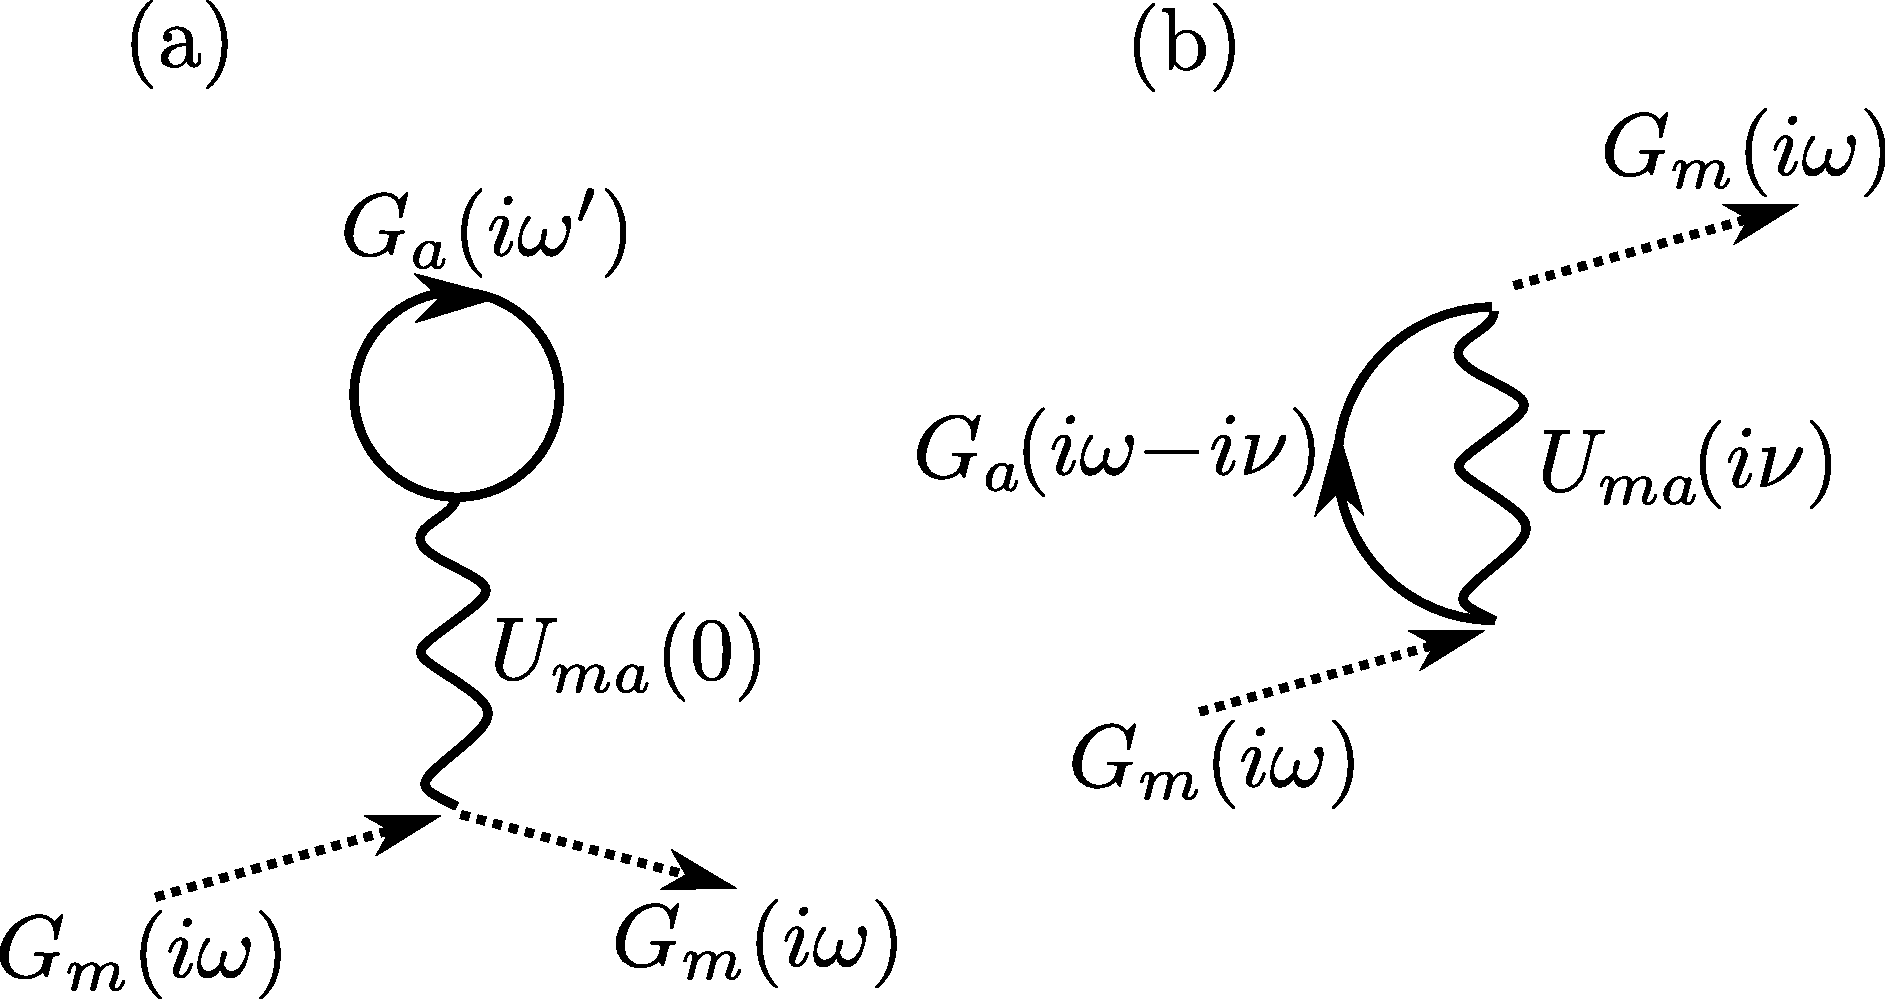
\includegraphics[width=0.6\textwidth]{figs/hfdiag.pdf}
\end{center}
\caption{The local Hartree (a) and Fock diagram (b)}
\label{fig:1storder_diags}
\end{figure}

In our case, when we only use a frequency dependent monopole term $F_0$,
all elements of the Coulomb interaction matrix have the same frequency
dependence and only differ in a constant spin- and orbital
dependent offset. This frequency dependence is described by
$K(\tau)$, as defined in section \ref{sec:gwdmft_cycle}.
$K'(\tau) = \partial_{\tau} K(\tau)$, has the following form at $\tau=0^+$
\begin{align}
 K'(0^+)
 &= \frac{1}{2}\left[ V_{bare} - U(0) \right] \\
  &= \frac{1}{2}\left[ U(\infty) - U(0) \right].
\end{align}
Since only the monopole term $F_0$ is frequency
dependent, this results in 
\begin{align}
 K'(0^+)
 &= \frac{1}{2}\left[ F_0(\infty) - F_0(0) \right]
\end{align}
which is spin- and orbital independent.

\subsection{Hartree Term}
We start by evaluating the Hartree diagram, shown in Fig. \ref{fig:1storder_diags} (a).
\begin{align}
\Sigma^{H}_{m\sigma}(i\omega)
&= \frac{1}{\beta} \sum_{a\sigma'}\sum_{i\omega_n'} U_{ma}(0) G_{a\sigma'}(i\omega_n') \\
&= \sum_{a\sigma'} U_{ma}(0) n_{a\sigma'} \\
&= \sum_{a\sigma'} \left[ U_{ma}(0) - U_{ma}(\infty) + U_{ma}(\infty) \right] n_{a\sigma'} \\
&= \sum_{a\sigma'} \left[ U_{ma}(0) - U_{ma}(\infty) \right] n_{a\sigma'} + \sum_{a\sigma'} U_{ma}(\infty)n_{a\sigma'} \\
&= -2K'(0^+)N + \sum_{a\sigma'} U_{ma}(\infty)n_{a\sigma'},
\end{align}
where $N=\sum_{a\sigma}n_{a\sigma}$.

\subsection{Fock Term}
We start by evaluating the Fock diagram, shown in Fig. \ref{fig:1storder_diags} (b).
\begin{align}
\Sigma^{F}_{m\sigma}(i\omega)
&= -\frac{1}{\beta} \sum_a \sum_{i\nu_n} J_{ma}(i\nu_n) G_{a\sigma}(i\omega_n-i\nu_n) \\
&= -\frac{1}{\beta} \sum_a\sum_{i\nu_n} \left[ J_{ma}(i\nu_n) - J_{ma}(\infty)+J_{ma}(\infty) \right] G_{a\sigma}(i\omega_n-i\nu_n) \\
%
&= -\frac{1}{\beta}\sum_a \sum_{i\nu_n} J_{ma}(\infty)G_{a\sigma}(i\omega_n-i\nu_n) \nonumber \\
& \hspace{0.5cm}  -\frac{1}{\beta} \sum_a \underbrace{\sum_{i\nu_n} \left[ J_{ma}(i\nu_n) - J_{ma}(\infty)\right] G_{a\sigma}(i\omega_n-i\nu_n)}_{\rightarrow 0 \mbox{ for }i\omega\rightarrow \infty} \\ 
%
&= - \sum_aJ_{ma}(\infty)n_{a\sigma}.
\end{align}

\subsection{Hartree+Fock Term}
This leads to the final expression
\begin{align}
\Sigma^{H}_{m\sigma}
&= -2K'(0^+)N + \sum_{a\sigma'} U_{ma}(\infty)n_{a\sigma'} \\
%
\Sigma^{F}_{m\sigma}
&= - \sum_aJ_{ma}(\infty)n_{a\sigma} \\
%
\Sigma^{HF}_{m\sigma}
&= -2K'(0^+)N + \sum_{a} U_{ma}(\infty)n_{a\bar{\sigma}} 
             + \sum_{a} [U_{ma}(\infty)-J_{ma}(\infty)]n_{a\sigma} .
\end{align}



%%%%%%%%%%%%%%%%%%%%%%%%%%%%%%%%%%%%%%%%%%%%%%%%%%%%%%%%%%%%%%%%%%%%%%%%%%%%%%%%%%%%%
%%%%%%%%%%%%%%%%%%%%%%%%%%%%%%%%%%%%%%%%%%%%%%%%%%%%%%%%%%%%%%%%%%%%%%%%%%%%%%%%%%%%%
%%%%%%%%%%%%%%%%%%%%%%%%%%%%%%%%%%%%%%%%%%%%%%%%%%%%%%%%%%%%%%%%%%%%%%%%%%%%%%%%%%%%%
%%%%%%%%%%%%%%%%%%%%%%%%%%%%%%%%%%%%%%%%%%%%%%%%%%%%%%%%%%%%%%%%%%%%%%%%%%%%%%%%%%%%%
%%%%%%%%%%%%%%%%%%%%%%%%%%%%%%%%%%%%%%%%%%%%%%%%%%%%%%%%%%%%%%%%%%%%%%%%%%%%%%%%%%%%%

\section{Non-local Hartree+Fock}
\label{sec:nonlocal_hartree_fock}
Here we want to evaluate the Hartree-Fock Selfenergy for a general
static but non-local interaction 
\begin{align}
v_{abcd}(q) = U_{abcd} + V_{abcd}(q),
\end{align}
where $U$ is a local interaction and $V$ the non-local part, e.g. a nearest-neighbour
interaction.


\subsection{Hartree Term}
We start by evaluating the Hartree diagram, shown in Fig. \ref{fig:1storder_diags} (a).
\begin{align}
\Sigma^{H}_{m\sigma}(k)
&= \frac{1}{N_k}\sum_{a\sigma'q} v_{mama}(0) n_{a\sigma'}(q) \\
&= \sum_{a} v_{mama}(0) N_{a},
\end{align}
where $N_{a}=\frac{1}{N_k}\sum_{\sigma q}n_{a\sigma}$.

\subsection{Fock Term}
We start by evaluating the Fock diagram, shown in Fig. \ref{fig:1storder_diags} (b).
\begin{align}
\Sigma^{F}_{m\sigma}(k)
&= -\frac{1}{N_k} \sum_{aq} v_{maam}(q) n^{\sigma}_a(k-q) \\
&= -\frac{1}{N_k} \sum_{aq} v_{maam}(k-q) n^{\sigma}_a(q).
\end{align}

\subsection{Hartree+Fock Term}
This leads to the final expression
\begin{align}
\Sigma^{HF}_{m\sigma}(k)
&= \sum_{a} v_{mama}(0) N_{a}
  -\frac{1}{N_k} \sum_{aq} v_{maam}(k-q) n^{\sigma}_a(q) \\
%
&= \frac{1}{N_k}\sum_{aq}\Big(  v_{mama}(0) n^{\bar{\sigma}}_{a}(q)
                        + \left[ v_{mama}(0) - v_{maam}(k-q) \right] n^{\sigma}_a(q) \Big).
\end{align}

Assuming that only the Hubbard and Hund's terms contribute and that the non-local
Hund's term is negligible
\begin{align}
v_{mama}(0) 
&= U_{mama} + V_{mama}(0) \\
&= U_{ma} + V_{ma}(0) \\
%
v_{maam}(k-q) 
&= U_{maam} + V_{maam}(k-q) \\
&= J_{ma} + V_{mm}(k-q)\delta_{am} ,
\end{align}
we get the following form
\begin{align}
\Sigma^{HF}_{m\sigma}(k)
&= \frac{1}{N_k}\sum_{aq}\Big(  \left[ U_{ma} + V_{ma}(0) \right] n^{\bar{\sigma}}_{a}(q) \nonumber\\
        & \hspace{1.95cm}   + \left[  U_{ma} + V_{ma}(0) - J_{ma} - V_{mm}(k-q)\delta_{am} \right] n^{\sigma}_a(q) \Big).\\
%
&= \sum_{a}\Big(  U_{ma} n^{\bar{\sigma}}_{a}  + \left[  U_{ma}- J_{ma} \right] n^{\sigma}_a \Big)
              +  \sum_{a}V_{ma}(0) N_a      \nonumber \\
       &\hspace{1cm} -\frac{1}{N_k}\sum_{q} V_{mm}(k-q) n^{\sigma}_m(q) 
\end{align}



%%%%%%%%%%%%%%%%%%%%%%%%%%%%%%%%%%%%%%%%%%%%%%%%%%%%%%%%%%%%%%%%%%%%%%%%%%%%%%%%%%%%%
%%%%%%%%%%%%%%%%%%%%%%%%%%%%%%%%%%%%%%%%%%%%%%%%%%%%%%%%%%%%%%%%%%%%%%%%%%%%%%%%%%%%%
%%%%%%%%%%%%%%%%%%%%%%%%%%%%%%%%%%%%%%%%%%%%%%%%%%%%%%%%%%%%%%%%%%%%%%%%%%%%%%%%%%%%%
%%%%%%%%%%%%%%%%%%%%%%%%%%%%%%%%%%%%%%%%%%%%%%%%%%%%%%%%%%%%%%%%%%%%%%%%%%%%%%%%%%%%%
%%%%%%%%%%%%%%%%%%%%%%%%%%%%%%%%%%%%%%%%%%%%%%%%%%%%%%%%%%%%%%%%%%%%%%%%%%%%%%%%%%%%%

\section{Local $\mu$ for frequency dependent interactions}
Following Werner, Millis PRL \textbf{99} 146404, when we apply a 
Lang-Firsov transformation to the Hubbard-Holstein Hamiltonian
that includes the electron-phonon coupling we obtain the new 
effective screened interaction and local chemical potential
as
\begin{align}
U_{scr}   &=   U - 2K'(0^+) \\
\mu_{scr} &= \mu - K'(0^+). \label{eq:mu_scr}
\end{align}
Now imagine a simple one-orbital model on the Bethe lattice at half-filling. The high-frequency
limit (Hartree-Fock term) of the Selfenergy is then given by
\begin{align}
\Sigma^{HF} &= Un - 2K'(0^+)N \nonumber \\
&= \frac{U}{2} - 2K'(0^+).
\end{align}
If electron-phonon coupling is absent, $K(0^+)=0$ and we regain
the standard expression $\Sigma^{HF} = U/2$.
On the Bethe lattice, the local interacting Green's function is given by
\begin{align}
G(i\omega)
&= \int\mathrm{d}\epsilon \, \frac{D(\epsilon)}{i\omega + \mu - \epsilon - \Sigma(i\omega_n)}.
\end{align}
From this equation we see that upon selfsonsistency, for half-filling $\mu$ has 
to be equal to the Hartree term of the Selfenergy
\begin{align}
\mu &= \frac{U}{2} - 2K'(0^+) \nonumber \\
&= \frac{1}{2} \left[ U - 2K'(0^+) \right] -K'(0^+) \nonumber \\
&= \frac{U_{scr}}{2} -K'(0^+) .
\end{align}
Again, if electron-phonon coupling is absent, we regain
the standard expression $\mu = U/2$ for half-filling. 

\textbf{If we now were to use this $\mu$ as an input for the Impurity solver, this would lead
to an inconsistency, since an additional factor of $K'(0^+)$ will be subtracted.}
Eq.\eqref{eq:mu_scr} requires the effective $\mu$ for the solver to be 
$U/2 - K'(0^+)$, while subtracting the additional factor would lead to 
$U/2 - 3K'(0^+)$.

\bigskip
This can be remedied in the following way:
\begin{itemize}
\item In practice, do not subtract but add a factor of $K'(0^+)$
to the $\mu$ that leads to half-filling of the local Green's function
(this is how TRIQS avoids this issue)
\item Add a factor of $2K'(0^+)$ by hand before passing it to the solver, which then subtracts
a factor of $K'(0^+)$ to get the right value
\item Increase the Hartree-Fock part of the Selfenergy by a factor of $2K'(0^+)$,
so the $\mu$ in the local Green's function will be correspondingly larger and lead to
the correct value after the solver has subtracted another factor
(This seems to be what is happening in ALPS).
\end{itemize}

 
%%%%%%%%%%%%%%%%%%%%%%%%%%%%%%%%%%%%%%%%%%%%%%%%%%%%%%%%%%%%%%%%%%%%%%%%%%%%%%%%%%%%%%%%%%%%%%%%
%%%%%%%%%%%%%%%%%%%%%%%%%%%%%%%%%%%%%%%%%%%%%%%%%%%%%%%%%%%%%%%%%%%%%%%%%%%%%%%%%%%%%%%%%%%%%%%%
%%%%%%%%%%%%%%%%%%%%%%%%%%%%%%%%%%%%%%%%%%%%%%%%%%%%%%%%%%%%%%%%%%%%%%%%%%%%%%%%%%%%%%%%%%%%%%%%
%%%%%%%%%%%%%%%%%%%%%%%%%%%%%%%%%%%%%%%%%%%%%%%%%%%%%%%%%%%%%%%%%%%%%%%%%%%%%%%%%%%%%%%%%%%%%%%%
%%%%%%%%%%%%%%%%%%%%%%%%%%%%%%%%%%%%%%%%%%%%%%%%%%%%%%%%%%%%%%%%%%%%%%%%%%%%%%%%%%%%%%%%%%%%%%%%
%%%%%%%%%%%%%%%%%%%%%%%%%%%%%%%%%%%%%%%%%%%%%%%%%%%%%%%%%%%%%%%%%%%%%%%%%%%%%%%%%%%%%%%%%%%%%%%%

\section{Product basis}
\label{sec:product_basis}

In the GW formalism we encounter objects such as the inverse dielectric function
\begin{align}
 \epsilon^{-1},
\end{align}
which is a two-particle operator. The standard way to specify the action of a two-particle operator
is to start from a complete orthonormal single-particle basis $\{ \ket{i} \}$, where
\begin{align}
 \braket{\vec{r} | i} &= \psi_i(\vec{r}),
\end{align}
with a complex valued function $\psi_i: R^3\rightarrow \mathbb{C}$.
Then one introduces a two-particle basis $\{ \ket{ij} \}$, which is composed of the single-particle states via
\begin{align}
\braket{\vec{r}\vec{r}' | ij} 
&= \Big( \bra{\vec{r}} \otimes \bra{\vec{r}'} \Big) \Big( \ket{i} \otimes \ket{j} \Big) \\
&= \psi_i(\vec{r})\psi_j(\vec{r}').
\end{align}
In this basis, any two-particle operator $A$ can be represented as a rank-4 tensor
by its action on the two-particle basis states
\begin{align}
A_{ijkl} &= \braket{ij | A | kl }  \\
&= \int \int \mathrm{d}\vec{r}\mathrm{d}\vec{r}' \, \psi^*_i(\vec{r})\psi^*_j(\vec{r}') 
                                          A(\vec{r},\vec{r}') \psi_l(\vec{r}')\psi_k(\vec{r}),
\end{align}
where we have assumed that 
\begin{align}
 \braket{\vec{r}\vec{r}' | A | \vec{r}''\vec{r}''' }
 &= A(\vec{r},\vec{r}') \delta(\vec{r}-\vec{r}'') \delta(\vec{r}'-\vec{r}'''),
\end{align}
which applies to the Coulomb interaction operator and all other operators we will consider here.

Our goal is to obtain a matrix (rank-2) representation of the two-particle operator $A$, so that we can 
define a proper inverse $A^{-1}$ or a multiplication $AB$ between these operators. 
This is usually done in two ways:

%%%%%%%%%%%%%%%%%%%%%%%%%%%%%%%%%%%%%%%%%%%%%%%%%%%%%%%%%%%%%%%%%%%%%%%%%%%%%
\subsection{Index combination}
In the two-particle basis the structure of the Tensor-elements
\begin{align}
 A_{ijkl} &= \braket{ij | A | kl } ,
\end{align}
suggests that we could also interpret each basis state as
\begin{align}
 \ket{a} := \ket{ ij } &= \ket{i}\otimes \ket{j} ,
\end{align}
with a single basis state $\ket{a}$, where the index $a$ now runs over $N^2$ values
if we have $N$ single particle states $\ket{i}$. In this notation, we can indeed write the tensor elements
as matrix elements
\begin{align}
 A_{ab} &= \braket{a | A | b } \\
 &= \braket{ij | A | kl }   \\
  &= A_{(ij)(kl)} .
\end{align}

\subsubsection{Properties and consistency}

The combination of the two left, the ``outgoing'' indices $ij$ and the right, the ``incoming'' $kl$ is in principle arbitrary.
We could also combine the indices $ik$ of the first partcile and $jl$ of the second particle. 
Though, the $(ij)(kl)$ combination should be preferrable, since it does not mix vectors $\ket{i}$ with their
dual counterpart $\bra{i}$. 

Furthermore, in cases where we want to apply this scheme, the tensor operations can indeed be rewritten
as a matrix multiplication in the combined ``ingoing-outgoing'' index notation. For example
the screened interaction $W$ is given by
\begin{align}
W_{ijkl} &= [ v + vPW ]_{ijkl} \\
&= v_{ijkl} + \sum_{mnop} v_{ijmn}P_{mnop}W_{opkl},
\end{align}
with the bare interaction $v$ and the polarization $P$. Using the combined index notation we get the representation
\begin{align}
W_{ab} &= W_{(ij)(kl)} \\
&= v_{(ij)(kl)} + \sum_{(mn)(op)} v_{(ij)(mn)}P_{(mn)(op)}W_{(op)(kl)} \\
&= v_{ab} + \sum_{cd} v_{ac}P_{cd}W_{da} \\
&= [v + vPW]_{ab},
\end{align}
where $vPW$ is to be understood as the matrix product of $v,P$ and $W$ in the combined index notation.

\subsubsection{Tensor inverse}

Now let us try to obtain a closed expression of $W$ satisfying this expression, which
is not possible in the 4-index tensor notation.
For this, we need to define first an object $\unity$ that serves as the identity element, which then will
allow us to poperly define an inverse of a matrix in the combined index notation.
The identity element should have the following property
\begin{align}
 \unity A &= A =  A \unity ,
\end{align}
where $A$ is a two-particle tensor, which means
\begin{align}
A_{(ij)(kl)} &= A_{ab} \\
&= [\unity A]_{ab} \\
&= \sum_c \unity_{ac} A_{ca} \\
&= \sum_{mn} \unity_{(ij)(mn)} A_{(mn)(kl)} .
\end{align}
From this we conclude that 
\begin{align}
 \unity_{(ij)(mn)} &= \delta_{im}\delta_{jn} \\
 \Rightarrow \unity_{ac} &= \delta_{ac},
\end{align}
which leads to the natural definition of the identity element in the combined index notation.
It can be directly seen that also $ A \unity = A$ is fulfilled.

From this we can define the inverse $A^{-1}$ as the standard matrix inverse in the combined index notation
that fulfills
\begin{align}
A^{-1}A &= AA^{-1} = \unity,
\end{align}
since
\begin{align}
[A^{-1}A]_{(ij)(kl)} &= [A^{-1}A]_{ab} \\
&= \delta_{ab} \\
&= \delta_{ik}\delta_{kl} \\
&= \unity_{(ij)(kl)}
\end{align}
With this, we can finally solve the equation above for the screened interaction
\begin{align}
 W &= v + vPW \\
 \Rightarrow (\unity - vP) W &= v \\
 \Rightarrow  W &=(\unity - vP)^{-1} v ,
\end{align}
By contruction, the tensor elements $W_{ijkl} =[(\unity - vP)^{-1} v]_{ijkl}$
will now satisfy the equation above for the screened interaction.

\subsubsection{Problems}
Possible problems are:
\begin{itemize}
\item A two-particle operator diagonal in position representation cannot be inverted
in the combined index-notation! This can be for example a purely local Coulomb interaction!

Consider 
\begin{align}
 \braket{\vec{r}\vec{r}' | A | \vec{r}''\vec{r}''' }
 &= A(\vec{r}) \delta(\vec{r}-\vec{r}') \delta(\vec{r}-\vec{r}'') \delta(\vec{r}'-\vec{r}'''),
\end{align}
and we assume that $A(\vec{r})=a>0$ constant, \textit{i.e.} it does not matter where the particles interact.
As long as their positions are identical they pick up a factor $a$.

This leads to the following tensor elements
\begin{align}
A_{ijkl} &= \braket{ij | A | kl }  \\
&= \int \int \mathrm{d}\vec{r}\mathrm{d}\vec{r}' \, \psi^*_i(\vec{r})\psi^*_j(\vec{r}') 
                                          a \delta(\vec{r}-\vec{r}') \psi_l(\vec{r}')\psi_k(\vec{r}) \\
&=a  \int \mathrm{d}\vec{r} \, \psi^*_i(\vec{r})\psi^*_j(\vec{r}) 
                                          \psi_l(\vec{r})\psi_k(\vec{r}) .
\end{align}
For the case of real wave functions we see that we always get a non-zero contribution when we pair 
two indices with one another, leading to an integral of the form
\begin{align}
a  \int \mathrm{d}\vec{r} \, \psi^2_m(\vec{r}) \psi^2_n(\vec{r}) \neq 0
\end{align}
For the example of $N=2$ single-particle states $\psi_i(\vec{r})$, we can choose two out of four indices to pair, then
the last one has to be paired with $N=2$ choices for the index, leading to 8 combinations which are at least non-zero.
In the combined index notation we then can arrive at the following matrix 
(\cng{Note: I have confirmed this numerically for a few basis sets})
\begin{align}
 A &= a
 \begin{pmatrix}
  c_1 & 0 & 0 & c_3 \\
  0   & c_2 & c_2 & 0 \\
  0 & c_2 & c_2 & 0 \\
  c_3 & 0 & 0 & c_4 
 \end{pmatrix},
\end{align}
where we can immediately see that this matrix cannot be inverted since two columns are linearly dependent (even identical).

\item A ``constant'' operator $A(\vec{r},\vec{r}')=c\neq 0$  can be inverted! (See discussion in next section)

\end{itemize}


%%%%%%%%%%%%%%%%%%%%%%%%%%%%%%%%%%%%%%%%%%%%%%%%%%%%%%%%%%%%%%%%%%%%%%%%%%%%%

\subsection{Aryasetiawan-style}
\subsubsection{Defining the new basis set}
We start by rewriting the equation for the tensor elements in the two-particle basis in the 
following way 
\begin{align}
 \braket{ij | A | kl }  
&= \int \int \mathrm{d}\vec{r}\mathrm{d}\vec{r}' \, \psi^*_i(\vec{r})\psi^*_j(\vec{r}') 
                                          A(\vec{r},\vec{r}') \psi_l(\vec{r}')\psi_k(\vec{r}) \\
%
&= \int \int \mathrm{d}\vec{r}\mathrm{d}\vec{r}' \, \psi^*_i(\vec{r})\psi_k(\vec{r}) 
                                          A(\vec{r},\vec{r}') \psi^*_j(\vec{r}')\psi_l(\vec{r}') \\
%
&= \int \int \mathrm{d}\vec{r}\mathrm{d}\vec{r}' \, \underbrace{ \Big( \psi^*_k(\vec{r}) \psi_i(\vec{r}) \Big)^* }_{B^*_a(\vec{r})}
                                          A(\vec{r},\vec{r}') \underbrace{ \psi^*_j(\vec{r}')\psi_l(\vec{r}') }_{B_b(\vec{r}' )} \\
&= \braket{ B_a | A | B_b } .
\end{align}
From these observation we see that we should define new basis states $\{ B_a \}$ by the product of the single-particle
states by
\begin{align}
 \braket{ \vec{r} | B_a } := \psi^*_i(\vec{r}) \psi_j(\vec{r}),
\end{align}
where the index $a:=a(i,j)$ lables the combination of the indices $i,j$. As a result, for a finite number of single-particle
states $N=\mathrm{dim}\{ \ket{i} \}$, we have $N^2$ new basis states $\{ B_a \}$, and could define the relation between the indices
as
\begin{align}
 a(i,j) := iN + j.
\end{align}
Though, the new set $\{ B_a \}$ is \textit{not} a basis, since it is overcomplete/linearly dependent and in addition not orthonormal.
For example if there exist at least two real single-particle basis functions $\psi_i,\psi_j$, one has 
\begin{align}
\psi_i(\vec{r})\psi_j(\vec{r}) = B_a(\vec{r}) = B_b(\vec{r}) = \psi_j(\vec{r})\psi_i(\vec{r}),
\end{align}
where $a\neq b$.
Also, for a states with indices $a(i,i)$ and $b(i,i)$, which leads to
\begin{align}
 \braket{B_a | B_b} &= \int \mathrm{d}\vec{r} \, \psi^*_i(\vec{r}) \psi_i(\vec{r}) \psi^*_j(\vec{r}) \psi_j(\vec{r}) \\
 &= \int \mathrm{d}\vec{r} \, |\psi_i(\vec{r})|^2 |\psi_j(\vec{r})|^2 
\end{align}
which is usually larger than zero for $a\neq b$, i.e. $i=j$ and not equal to $1$ in case $a=b$, i.e. $i\neq j$.

The overlap matrix for the new set $\{ B_a \}$ is therefore different from the unit matrix.
If we define 
\begin{align}
 v := 
 \begin{pmatrix}
%   \ket{B_1}\\ \ket{B_2}\\\ket{B_3}\\ \vdots \\ \ket{B_{N^2}}
\ket{B_1} & \ket{B_2} & \ket{B_3}& \cdots & \ket{B_{N^2}}  
 \end{pmatrix},
\end{align}
then the overlap matrix can be written as
\begin{align}
O &= v^{\dagger}\cdot v,
\end{align}
since
\begin{align}
O_{ab} &= (v^{\dagger}\cdot v)_{ab} \\
 &= \braket{B_a | B_b} .
\end{align}
Due to the overcompleteness, some columns of $O$ will not be linear independent, i.e. some of the Eigenvalues 
$\lambda_i$ of $O$ will be equal to zero.

\subsubsection{Reduction of the basis set and reorthonormalization}

After diagonalizing $O$ to obtain the Eigenvectors $o_1,o_2,...,o_{N^2}$, we throw away the ones with Eigenvalue zero 
and set up the matrices
\begin{align}
 U &=
 \begin{pmatrix}
  o_1 & o_2 & o_3 & \cdots o_{N_r}
 \end{pmatrix} \in \mathbb{C}^{N^2 \times N_r},
\end{align}
where $N_r \leq N^2$ is the number of Eigevectors with nonzero Eigenvalue,
and
\begin{align}
 D^{-1/2} &:= \mathrm{diag}( {\lambda_1}^{-1/2}, \ {\lambda_2}^{-1/2}, \ {\lambda_3}^{-1/2}, \ \cdots,\ {\lambda_{N_r}}^{-1/2}  ) 
 \in \mathbb{R}^{N_r \times N_r},
\end{align}
where $\lambda_i$ are the nonzero Eigenvalues of $O$.


The elements of the following vector
\begin{align}
\tilde{v} := vUD^{-1/2} ,
\end{align}
will then yield a new set of $N_r$ basis functions which are complete and orthonormal, as can be seen from
the new overlap matrix
\begin{align}
\tilde{O} &= \tilde{v}^{\dagger}\cdot \tilde{v} \\
&= D^{-1/2}U^{\dagger} (v^{\dagger} \cdot v) UD^{-1/2} \\
&= D^{-1/2} \underbrace{U^{\dagger} O U}_{=D} D^{-1/2} \\
&= \unity  \in \mathbb{R}^{N_r \times N_r}.
\end{align}

\textit{Remark:}
To reduce the size of the basis for computational efficiency, one can also exclude Eigenvectors with a finite, 
but small Eigenvalue, i.e. below some treshhold $\delta > \lambda_i$.
Then the new basis will only be approximately complete and orthonormal, but the error can be controlled by choosing
$\delta$ sufficiently small.

\subsubsection{Product basis matrix elements}

After having obtained the new complete orthonormal basis $\{ \tilde{B}_a  \}$, the matrix elements
of any two-particle operator are then given as
\begin{align}
A_{ab}
&= \braket{ \tilde{B}_a | A | \tilde{B}_b } \\
&= \int \int \mathrm{d}\vec{r}\mathrm{d}\vec{r}' \,  \tilde{B}^*_a(\vec{r})  A(\vec{r},\vec{r}') \tilde{B}_b(\vec{r}').
\end{align}
The representation of $A$ in the product basis is then given as
\begin{align}
A &= \sum_{a,b} \ket{\tilde{B}_a}A_{ab}\bra{\tilde{B}_b} .
\end{align}
or in the position representation \cng{DOES THIS MAKE SENSE?}
\begin{align}
 A(\vec{r},\vec{r}') &= \sum_{a,b} \braket{\vec{r}|\tilde{B}_a} A_{ab}\braket{\tilde{B}_b|\vec{r}'} \\
 &= \sum_{a,b} \tilde{B}_a(\vec{r}) A_{ab}\tilde{B}^*_b(\vec{r}') .
\end{align}
\cng{CHECK HERE IF BOTH REPRESENTATIONS LEAD TO THE SAME RESULT!!! The product basis should recover
the right A(r-r'), shouldn't it? (I think so...) Can we actually prove this?}


\subsubsection{Switching between the product and the two-particle basis}
If we want to obtain the original tensor representation of a two-particle operator in the 
product basis, we have to evaluate \cng{DOES THIS MAKE SENSE?}
\begin{align}
A_{ijkl} &= \braket{ij | A | kl }  \\
&= \int \int \mathrm{d}\vec{r}\mathrm{d}\vec{r}' \, \psi^*_i(\vec{r})\psi^*_j(\vec{r}') 
                                          A(\vec{r},\vec{r}') \psi_l(\vec{r}')\psi_k(\vec{r}) \\
&= \sum_{a,b}\int \int \mathrm{d}\vec{r}\mathrm{d}\vec{r}' \, \psi^*_i(\vec{r})\psi^*_j(\vec{r}') 
         \tilde{B}_a(\vec{r}) A_{ab}\tilde{B}^*_b(\vec{r}') \psi_l(\vec{r}')\psi_k(\vec{r}).
\end{align}
The other way round, if we have a two-particle operator given in the two-particle basis, the product basis
representation can be obtained by
\begin{align}
A_{ab}
&= \braket{ \tilde{B}_a | A | \tilde{B}_b } \\
&= \int \int \mathrm{d}\vec{r}\mathrm{d}\vec{r}' \,  \tilde{B}^*_a(\vec{r})  A(\vec{r},\vec{r}') \tilde{B}_b(\vec{r}') \\
&=\sum_{ijkl} \int \int \mathrm{d}\vec{r}\mathrm{d}\vec{r}' \,  \tilde{B}^*_a(\vec{r})  
    \psi_i(\vec{r})\psi_j(\vec{r}') A_{ijkl} \psi^*_l(\vec{r}')\psi^*_k(\vec{r}) \tilde{B}_b(\vec{r}') .
\end{align}

If we define the "overlap" between the original two-particle
basis and the new product basis by
\begin{align}
P_{ij,a}
&= \int  \mathrm{d}\vec{r}\, \psi^*_i(\vec{r}) \tilde{B}_a(\vec{r}) \psi_j(\vec{r}) ,
\end{align}
we can write the transformation as follows
\begin{align}
A_{ijkl} &= \braket{ij | A | kl }  \\
&= \sum_{a,b}\int \int \mathrm{d}\vec{r}\mathrm{d}\vec{r}' \, \psi^*_i(\vec{r}) \tilde{B}_a(\vec{r}) \psi_k(\vec{r})
      \   A_{ab}\ \psi_l(\vec{r}') \tilde{B}^*_b(\vec{r}') \psi^*_j(\vec{r}') \\
&= \sum_{a,b} P_{ik,a} A_{ab} P^*_{lj,b}
\end{align}
and the other way round
\begin{align}
A_{ab}
&=\sum_{ijkl} \int \int \mathrm{d}\vec{r}\mathrm{d}\vec{r}' \,  \psi_i(\vec{r}) \tilde{B}^*_a(\vec{r}) \psi^*_k(\vec{r}) 
     \ A_{ijkl}\  \psi^*_l(\vec{r}') \tilde{B}_b(\vec{r}') \psi_j(\vec{r}') \\
%
&= \sum_{ijkl} P^*_{ik,a}  A_{ijkl} P_{lj,b}.
\end{align}
Here we see that we cannot write this transformation as a simple matrix equation
if we were to combine the two first $(ij)$ and last $(kl)$ indices.

For the special case of 
\begin{align}
A_{ijkl} &= \braket{ij|A|ij}\delta_{ik}\delta_{jl} + \braket{ij|A|ji}\delta_{il}\delta_{jk} \\
&= U_{ij} \delta_{ik}\delta_{jl} + J_{ij}\delta_{jk},
\end{align}
we get the following form
\begin{align}
U_{ij} &= \sum_{a,b} P_{ii,a} A_{ab} P^*_{jj,b} \\
J_{ij} &= \sum_{a,b} P_{ij,a} A_{ab} P^*_{ij,b} \\
A_{ab} &= \sum_{ij} P^*_{ii,a}  U_{ij} P_{jj,b} + P^*_{ij,a}  J_{ij} P_{ij,b}.
\end{align}

% \begin{align}
%  \braket{ii | A | jj }  
% &= \int \int \mathrm{d}\vec{r}\mathrm{d}\vec{r}' \, \psi^*_i(\vec{r})\psi_j(\vec{r}) 
%                                           A(\vec{r},\vec{r}') \psi^*_i(\vec{r}')\psi_j(\vec{r}')
% \end{align}
% 
% \begin{align}
%  \braket{ij | A | ij }  
% &= \int \int \mathrm{d}\vec{r}\mathrm{d}\vec{r}' \, \psi^*_i(\vec{r})\psi_i(\vec{r}) 
%                                           A(\vec{r},\vec{r}') \psi^*_j(\vec{r}')\psi_j(\vec{r}')
% \end{align}
% 
% \begin{align}
%  \braket{ij | A | ji }  
% &= \int \int \mathrm{d}\vec{r}\mathrm{d}\vec{r}' \, \psi^*_i(\vec{r})\psi_j(\vec{r}) 
%                                           A(\vec{r},\vec{r}') \psi^*_j(\vec{r}')\psi_i(\vec{r}')
% \end{align}

\subsubsection{Tensor inverse}

Since in the product basis any two-particle operator can now be
represented as a matrix/rank-2 tensor, we can finally define its inverse $\tilde{A}^{-1}$ as the standard Matrix inverse, which then in the product basis fulfils the property
\begin{align}
 (\tilde{A}^{-1}A)_{ab}
&= \braket{ \tilde{B}_a | \tilde{A}^{-1}A | \tilde{B}_b } \\
&= \delta_{ab}.
\end{align}
In the position representation
\begin{align}
\braket{\vec{r} | \tilde{A}^{-1}A | \vec{r}' }
 &= \sum_{a,b} \braket{\vec{r}|\tilde{B}_a} (\tilde{A}^{-1}A)_{ab}\braket{\tilde{B}_b|\vec{r}'} \\
%
&= \sum_{a,b} \braket{\vec{r}|\tilde{B}_a} \delta_{ab} \braket{\tilde{B}_b|\vec{r}'} \\
&= \sum_{a} \braket{\vec{r}|\tilde{B}_a} \braket{\tilde{B}_a|\vec{r}'} \\
&= \braket{\vec{r}|\vec{r}'} \\
&= \delta(\vec{r}-\vec{r}'),
\end{align}
if the product basis is complete.

%\braket{\vec{r}|\tilde{B}_a} A_{a\braket{\tilde{B}_b|\vec{r}'}

\subsubsection{Problems}
Possible problems are:
\begin{itemize}
 \item A ``constant'' tensor of the form $A(\vec{r},\vec{r}')=c\neq 0$ cannot be inverted! 
 \cng{I'm not sure, this is maybe correct behaviour?}

 Let us assume we obtain a final basis state $\ket{\tilde{B}_o}$ in a one-dimensional system
 which is a real odd function in position representation, \textit{i.e.}
 \begin{align}
  \tilde{B}_o(r) &= -\tilde{B}_o(-r).
 \end{align}
For a constant tensor this leads to the following
 \begin{align}
A_{ab}
&=c \int \int \mathrm{d}\vec{r}\mathrm{d}\vec{r}' \,  \tilde{B}^*_a(\vec{r})  \tilde{B}_b(\vec{r}') \\
&=c \left(\int \mathrm{d}\vec{r} \, \tilde{B}^*_a(\vec{r}) \right) \left( \int \mathrm{d}\vec{r}'\,  \tilde{B}_b(\vec{r}'), \right),   
\end{align}
\textit{i.e.} the two integrations over the basis states decouple, and everytime $a$ or $b$ is equal to the
real odd function $\tilde{B}_o$, we obtain zero. Therefore, the $o$-th column and row is equal to zero.
Which means, we have at least one Eigenvalue equal to zero and, therefore, the tensor
in the product basis cannot be inverted.

\item The ``identity'' tensor of the form $\braket{ij|A|kl}=\delta_{ik}\delta_{jl}$ 
cannot be inverted! 
This can be seen from
\begin{align}
A_{ab}
&= \braket{ \tilde{B}_a | A | \tilde{B}_b } \\
&=\sum_{ijkl} \int \int \mathrm{d}\vec{r}\mathrm{d}\vec{r}' \,  \tilde{B}^*_a(\vec{r})  
    \psi_i(\vec{r})\psi_j(\vec{r}') A_{ijkl} \psi^*_l(\vec{r}')\psi^*_k(\vec{r}) \tilde{B}_b(\vec{r}') \\
 &=\sum_{ij} \int \int \mathrm{d}\vec{r}\mathrm{d}\vec{r}' \,  \tilde{B}^*_a(\vec{r})  
 \psi_i(\vec{r})\psi_j(\vec{r}') \psi^*_j(\vec{r}')\psi^*_i(\vec{r}) \tilde{B}_b(\vec{r}') \\
  &=\sum_{ij} \left(\int \mathrm{d}\vec{r} \,  \tilde{B}^*_a(\vec{r})  
 |\psi_i(\vec{r})|^2 \right)
 \left(\int \mathrm{d}\vec{r}' \,  \tilde{B}_b(\vec{r}')  
 |\psi_j(\vec{r}')|^2 \right).
\end{align}
 If one basis function $\tilde{B}_a(\vec{r})$ is an odd function, 
 the full column $a$ and row $a$ will be zero, so 
 we have at least one Eigenvalue equal to zero and, therefore, the tensor
in the product basis cannot be inverted.
\end{itemize}

\subsection{Simple example}
We take a complete basis set of dimension 2 given by
\begin{align}
 \braket{x | \psi_1 } = \frac{1}{\sqrt{2}} \\
 \braket{x | \psi_2 } = x\sqrt{\frac{3}{2}}, 
\end{align}
which form an orthonormal basis on the set $H= [-1,1]$:
\begin{align}
 \int_{-1}^{1} \psi_1(x)\psi_1(x) \, \mathrm{d}x
 &= \frac{1}{2} [ x ]_{-1}^1 = 1 \\
%
 \int_{-1}^{1} \psi_2(x)\psi_2(x) \, \mathrm{d}x
 &= \frac{3}{2} \left[\frac{1}{3} x^3 \right]_{-1}^1 = 1 \\
%
 \int_{-1}^{1} \psi_1(x)\psi_2(x) \, \mathrm{d}x
 &= \frac{\sqrt{3}}{2} \left[\frac{1}{2}x^2 \right]_{-1}^1 = 0 .
\end{align}
Of course this basis set is not complete to represent
all possible real functions on $H$ but we restrict here to 
the Hilbert space spanned by all functions that 
can be generated from $\psi_1,\psi_2$. For example, this corresponds
to choosing a correlated subspace in DFT+DMFT.

We now choose the two-particle operator
\begin{align}
A(x,y) &= x+y.
\end{align}
Calculating the matrix elements of the operator by
\begin{align}
 A_{ijkl} &= \braket{ij|A|kl} \\
 &= \int_{-1}^{1} \psi_i(x) \psi_j(y) A(x,y) \psi_k(x) \psi_l(y) \, \mathrm{d}x\mathrm{d}y,
\end{align}

which leads to the following matrix representation


%%%%%%%%%%%%%%%%%%%%%%%%%%%%%%%%%%%%%%%%%%%%%%%%%%%%%%%%%%%%%%%%%%%%%%%%%%%%%%%%%%%%%
%%%%%%%%%%%%%%%%%%%%%%%%%%%%%%%%%%%%%%%%%%%%%%%%%%%%%%%%%%%%%%%%%%%%%%%%%%%%%%%%%%%%%
%%%%%%%%%%%%%%%%%%%%%%%%%%%%%%%%%%%%%%%%%%%%%%%%%%%%%%%%%%%%%%%%%%%%%%%%%%%%%%%%%%%%%
%%%%%%%%%%%%%%%%%%%%%%%%%%%%%%%%%%%%%%%%%%%%%%%%%%%%%%%%%%%%%%%%%%%%%%%%%%%%%%%%%%%%%
%%%%%%%%%%%%%%%%%%%%%%%%%%%%%%%%%%%%%%%%%%%%%%%%%%%%%%%%%%%%%%%%%%%%%%%%%%%%%%%%%%%%%

\section{Non-causality of the impurity hybridization}
\label{sec:noncausal_hyb}

\subsection{Initial thoughts and relation to the doublecounting}

It is interesting to investigate the effects of the Doublecounting
used in GW+DMFT on the hybridization function.
\begin{align}
\Delta(i\omega) &= i\omega + \mu - \mathscr{G}_{bath}^{-1}(i\omega) \\
&= i\omega + \mu - G_{loc}^{-1}(i\omega) - \Sigma_{imp}(i\omega).
\end{align}
The hybridization function $\Delta(i\omega_n)$ effectively encodes the bath
of the impurity and thus carries the information about the surrounding lattice.
In standard lattice DMFT without extensions this bath is purely noninteracting
and just given by the free lattice dispersion.

In LDA+DMFT, since we perform a downfolding from the full space
to a low-energy subspace, where the bath now encodes all information 
about the outer space, the bath is no longer non-interacting.
It contains all interaction effects residing in the outer space
on the DFT level. Thus, which is an important point!, purely
on a one-particle level, i.e. the hybridization function can still 
be written like a non-interacting lattice hybridization
\begin{align}
\Delta(i\omega) &= \sum_{kj} \frac{|V^j_k|^2}{i\omega_n - \epsilon_k^j}
\end{align}
From the definition 
$\Delta(i\omega) = i\omega + \mu - G_{loc}^{-1}(i\omega) - \Sigma_{imp}(i\omega)$
I think it makes sense that $\Delta(i\omega)$ can also encode an interacting
bath, that contains interactions in the outer space,
since it is basically the local lattice Green's function minus the local interactions.
\textbf{(But I need to go through
the DMFT derivation again...)}

\bigskip

In GW+DMFT the hybridization or resp. the bath can become even "more interacting",
depending on what kind of doublecounting we use:
\begin{itemize}
\item If the full local GW Selfenergy is subtracted as the doublecounting
\[
\Sigma^{DC} = \left[GW \right]_{loc},
\]

then basically also all the local Selfenergy effects in $G_{loc}$ are 
originating purely from $\Sigma_{imp}$, since 
\begin{align}
 G(k,i\omega_n) 
 &= \left[ \unity(i\omega_n+\mu ) -H^{DFT}(k) + v^{XC}(k) \right. \nonumber \\
          & \hspace{1cm}- \Sigma^{GW}(k,i\omega_n) 
          + \Sigma^{DC}(i\omega_n)
          \left. - \Sigma^{imp}(i\omega_n)
           \right]^{-1} 
%
\end{align}
 This part is then subtracted
when creating $\Delta(i\omega)$, thus there is effectively no remainder of a 
local Selfenergy in $\Delta(i\omega)$. This usually gives a fast
decaying high-frequency tail of $\Delta(i\omega)$.

\item If only the impurity contribution is subtracted from GW
\[
\Sigma^{DC} = G_{loc}W_{loc},
\]

then the local Selfenergy effects in $G_{loc}$ are 
originating not only from $\Sigma_{imp}$ BUT there is also
a contribution from GW since
\[
\sum_k \Sigma^{GW}(k) - \Sigma^{DC} \neq 0,
\]
that stems from the contributions of nonlocal propagators
to the local Selfenergy, that are not captured by DMFT.
As an example we compare the local GW Selfenergy, the Doublecounting term
and the remaining component in Fig.~\ref{fig:Sigma_compare_loc_GW_DC}
for SrVO$_3$:
\begin{figure}[h]
\begin{center}
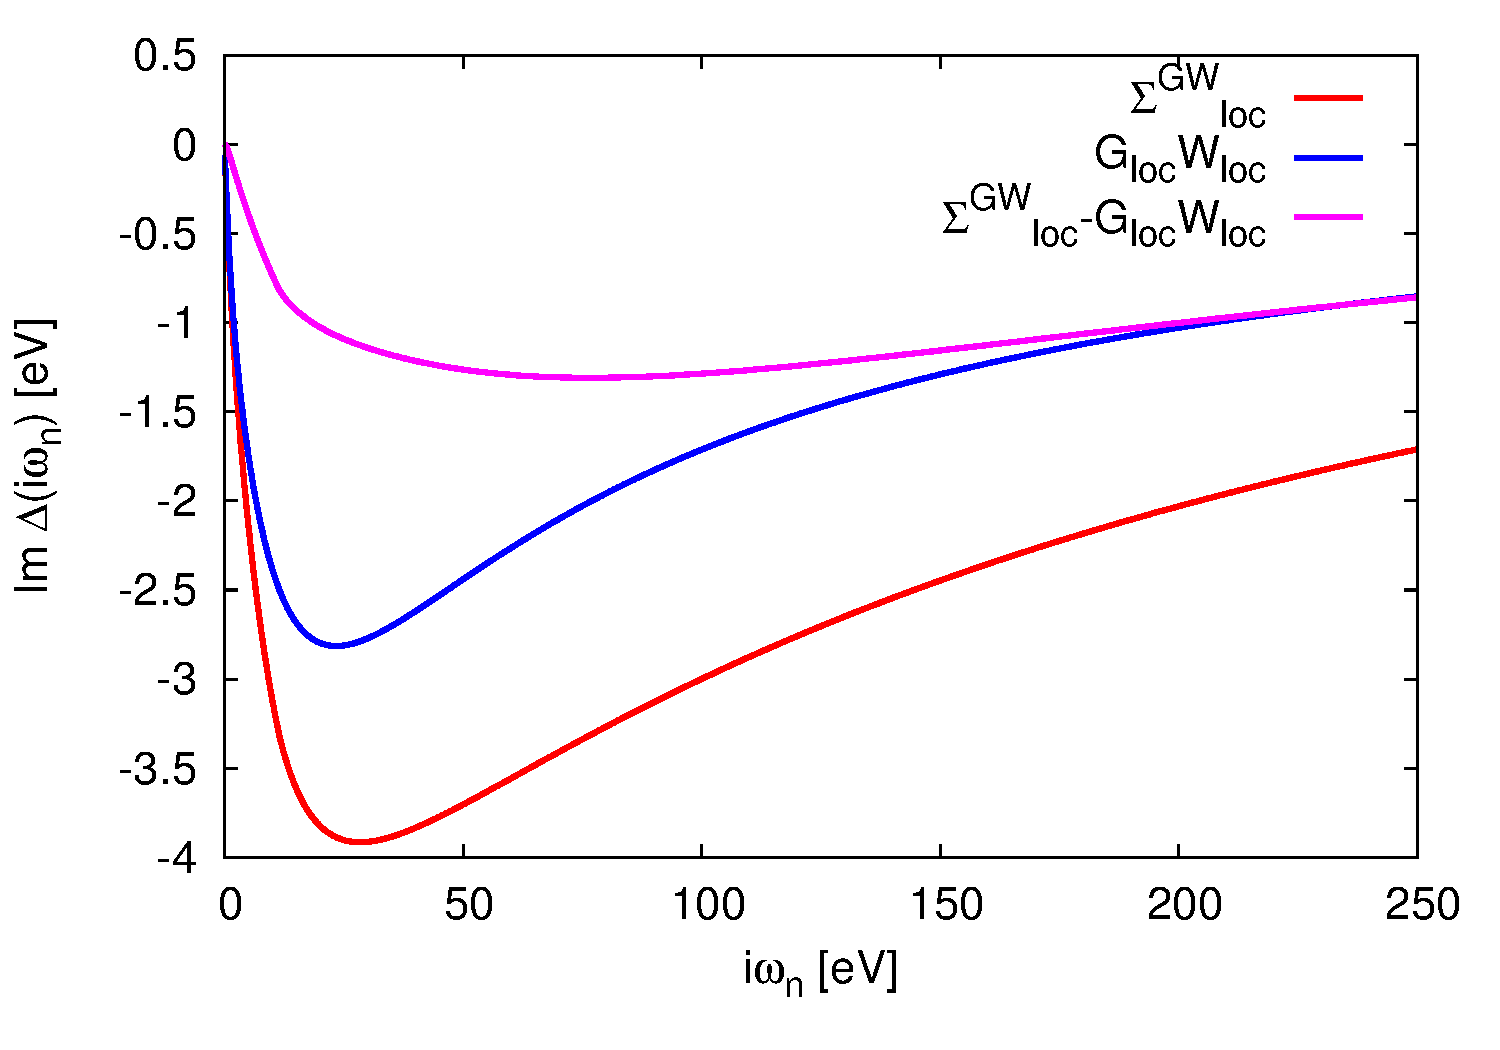
\includegraphics[width=0.7\textwidth]{figs/SrVO3_s_gw_DC.pdf} 
\end{center}
\caption{This plot shows the local GW Selfenergy (averaged over k-points)
in comparison to the $G_{loc}W_{loc}$ doublecounting, which only includes
the GW contribution on the impurity, and therefore is smaller
than the local GW part.
The difference between the two (pink line) is what remains in the local
GW Selfenergy from non-local propagators. It is still comparable in
size to the GW Selfenergy and decays similarly slow, so still
contains many high-energies features.}
\label{fig:Sigma_compare_loc_GW_DC}
\end{figure}

This has the effect that now there is effectively a remainder of a 
local GW Selfenergy in $\Delta(i\omega)$. This leads to very slowly
decaying high-frequency tail of $\Delta(i\omega)$, since the remaining
Selfenergy still creates features (plasmonic-like?) features at higher energy,
which are now encoded in the effective DMFT bath.
Now the hybridization function can no longer 
be written like a non-interacting lattice hybridization
\begin{align}
\Delta(i\omega) &= \sum_{kj} \frac{|V^j_k|^2}{i\omega_n - \epsilon_k^j}
\end{align}
But I think this is also the case for the other doublecounting?
Since it contains nonlocal components of the GW Selfenergy?...
But here in this case the bath carries information about a local Selfenergy
that also resides on the impurity, but cannot be generated from only
the local interactions on the impurity!!
The meaning is not clear to me yet...

\bigskip

As an example we show the hybridization function for SrVO$_3$
in Fig.~\ref{fig:hybrid_comp_SVO} calculated from a GW+DMFT calculation
with the two different doublecountings.
We immediately see that the energy scales of the impurity bath
are different by orders of magnitude. 

\begin{figure}[h]
\begin{center}
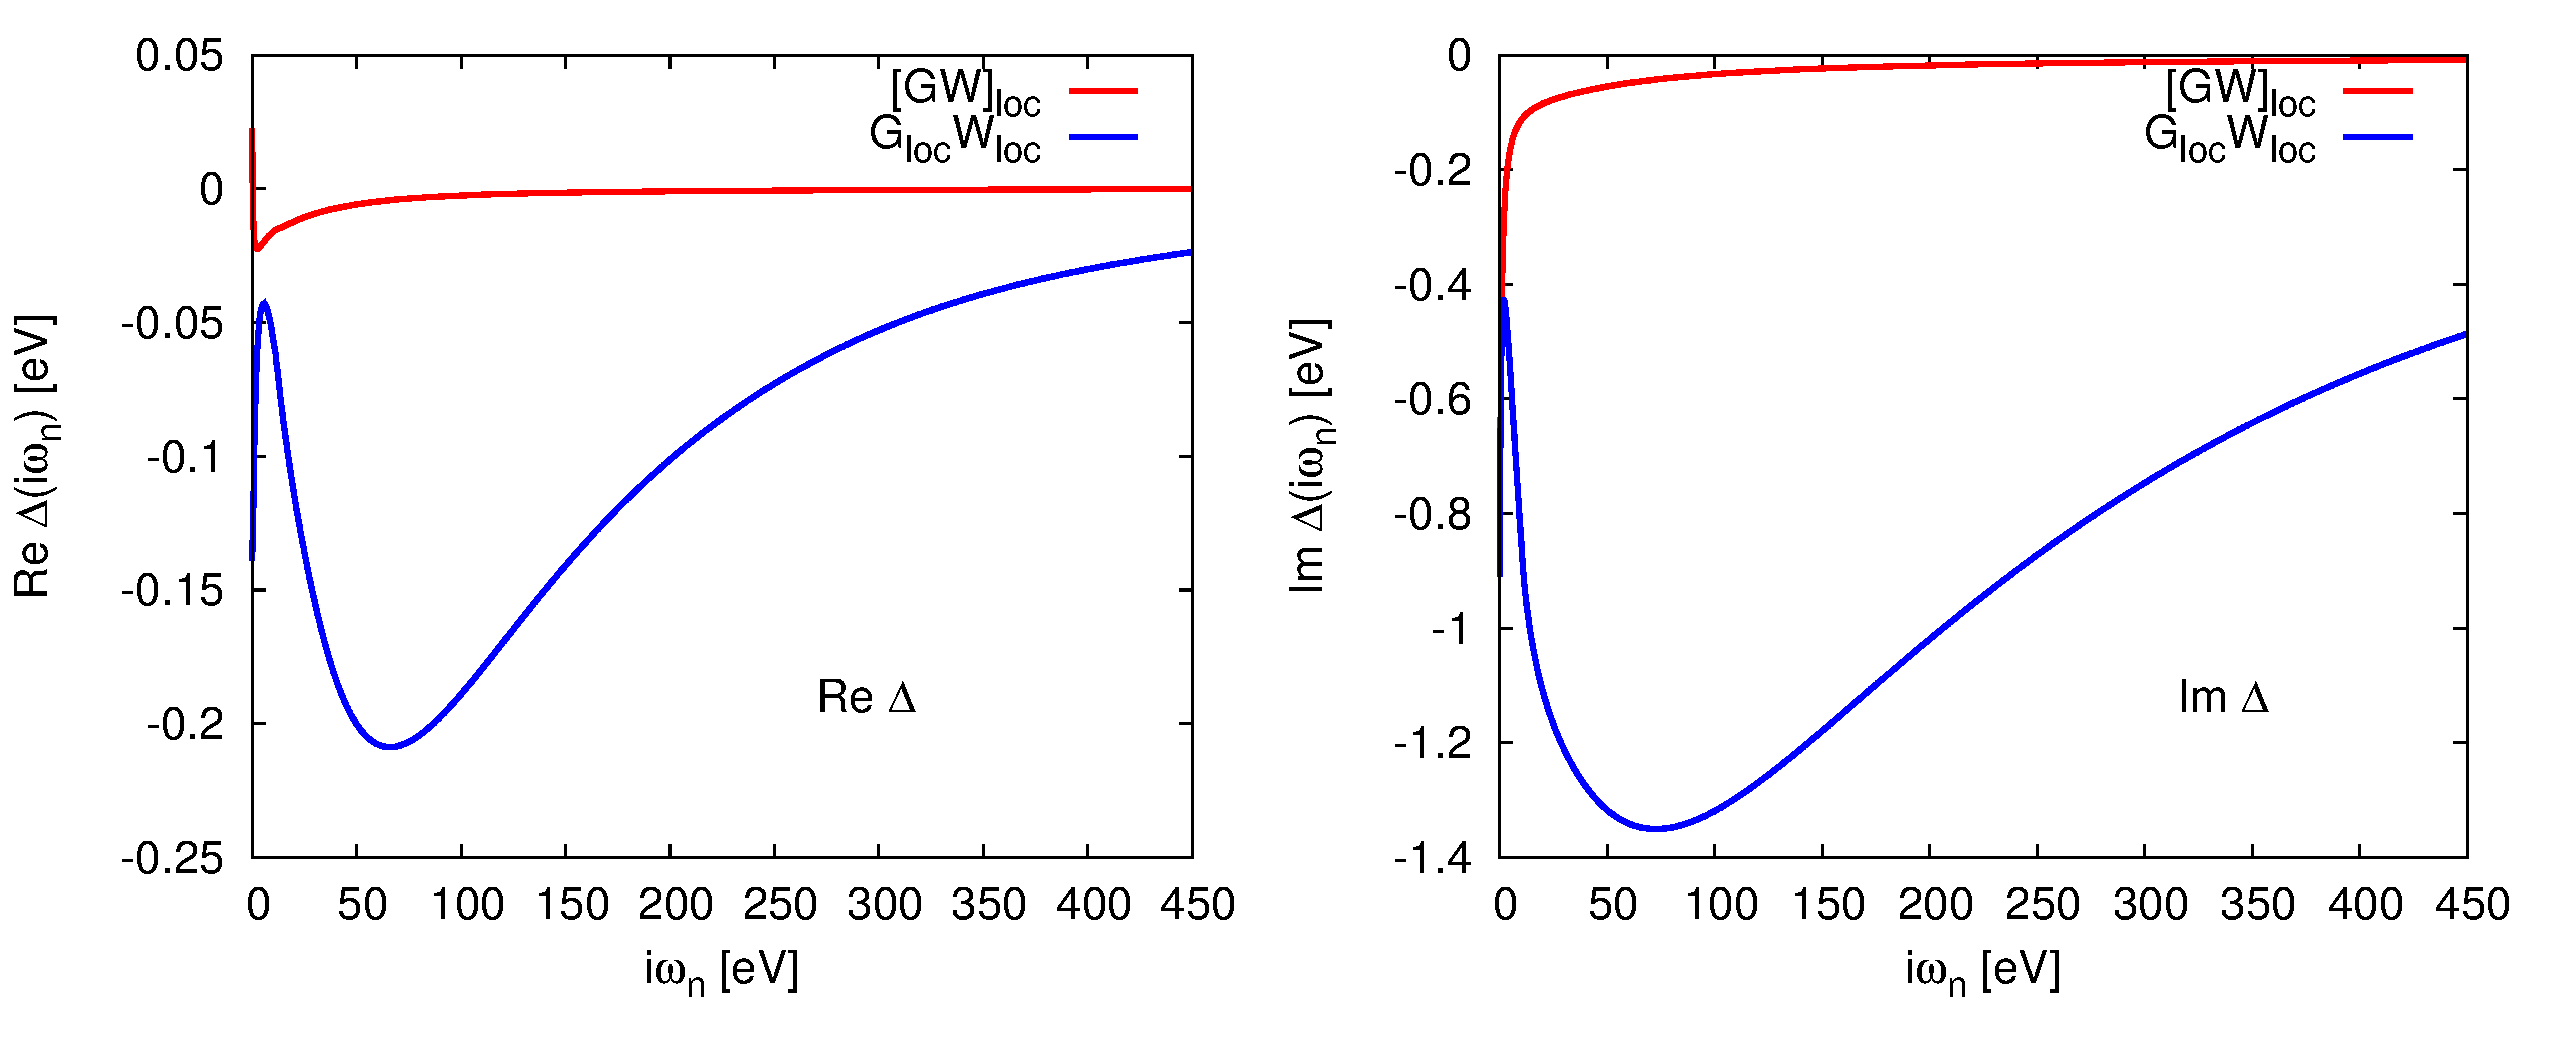
\includegraphics[width=1\textwidth]{figs/SrVO3_hybrid_dc_comp.pdf} 
\end{center}
\caption{This plot shows the impurty hybridization function
$\Delta(i\omega_n)$ for SrVO$_3$, for the two different types
of doublecounting that we use. 
For the $[GW]_{loc}$ Doublecounting, the full local part of the GW
Selfenergy  is substracted, while for the $G_{loc}W_{loc}$ Doublecounting
only the impurity GW contribution is subtracted. Therefore, 
there is a local Selfenergy component remaining in the hybridization
function, giving rise to high energy features in the bath, that can 
be identified as very slowly decaying tails in $\Delta(i\omega_n)$.}
\label{fig:hybrid_comp_SVO}
\end{figure}
\end{itemize}

The problem becomes even more prominent if ``non-correlated'' states
are included in the considered energy window or Wannier space.
In NiO one usually creates a low-energy model comprising the Ni-$d$ and O-$p$
states that hybridize significantly with each other.
This means there are off-diagonal $d-p$ elements in the Hamiltonian $H$, 
the exchange-correlation potentail $V_{xc}$ and the 
GW Selfenergy $\Sigma^{GW}$.
Thus, when creating the local Green's function
\begin{align}
 G(k,i\omega_n) 
 &= \left[ \unity(i\omega_n+\mu ) -H^{DFT}(k) + v^{XC}(k) \right. \nonumber \\
          & \hspace{1cm}- \Sigma^{GW}(k,i\omega_n) 
          + \Sigma^{DC}(i\omega_n)
          \left. - \Sigma^{imp}(i\omega_n)
           \right]^{-1} ,
\end{align}
the $G_{dd}$ elements will receive some contribution originating 
from $\Sigma_{pp}$, since the offdiagonal terms due to the orbital
hybridization couple them.
If now only the Ni $d$ orbitals are treated, the Hybridization function
is given by
\begin{align}
\Delta(i\omega) 
&= i\omega + \mu - G_{loc}^{-1}(i\omega) - \Sigma_{dd}(i\omega),
\end{align}
and the $d-d$ components will still contain significant high-energy features
due to the effect of the $\Sigma_{pp}$ and $\Sigma_{pd}$
components. This can be clearly seen in Fig.
\cng{INCLUDE FIGURE}

We observe long high-energy tails in $-\mathrm{Im}\Delta(\omega)$,
in addition to plasmonic features also at lower energies. 
Physically this is reasonable, since we have only excluded the
effective $d-d$ Selfenergy contributions due to the interactions.
But it is not clear to me whether this is the correct
bath for the DMFT impurity model. The bath now explicitely
has significant interaction effects included, where the high-energy
features introduce significant additional kinetic energy
in the $d$ orbitals, which in general will lead to greatly reduced
correlation effects. For example,
a GW+DMFT calculation for NiO in this $d-p$ model is
still metallic, while in a standard DFT+DMFT 
it opens a $\sim 4$~eV gap. But the origin of the metallicity
is not clear yet, but the additional kinetic energy 
for sure contributes to the decrease in correlation effects.
Whether a proper inclusing of the $U_{dp}$ interaction
is needed, is still under active investigation. 

If we were to solve the full local $d-p$ system, where we
can calculate the local Selfenergy including all 
$d-d$, $d-p$ and $p-p$ elements, the $\Sigma_{imp}$ that is subtracted
from $G_{loc}$ to create the Hybridization function would indeed remove
all these contributions. The result for NiO is shown in Fig.
\cng{ADD FIGURE}

We see that we still retain the high energy features in the local
hybridization function even when the full local $\Sigma$ matrix is subtracted.
This tells us that 

\cng{IS THIS EVEN CAUSAL?}



\subsection{Causality definition, mathematical properties}

\textbf{Definition:}
A Green's function $G$, Selfenergy $\Sigma$, or other functions $F$ derived from them
is called \textit{causal}, if 
\begin{align}
\mathrm{Im}F(\omega) \leq 0 \  \forall \omega \in \mathbb{R}.
\end{align}
\cng{Does it have to be strictly negative? }
For example, if a Green's function is causal then its related
spectral function $A(\omega) = -\mathrm{Im}G(\omega)/\pi \geq 0$.

\textbf{Theorem:}
A function $F(\omega)$ is causal if and only if its corresponding
transform $F(\tau)$ to the imaginary time interval $(0,\beta)$
has only negative definite even derivatives, i.e.
\begin{align}
F(\omega) \mbox{ causal }
%
\Leftrightarrow
%
\frac{\partial^{2n} }{\partial \tau^{2n}} F(\tau) \leq 0 \ \forall n\in\mathbb{N}.
\end{align}
\cng{Maybe its strictly negative?}

\textbf{Proof:}

$\Rightarrow$: Assume that $\mathrm{Im}F(\omega) \leq 0 \  \forall \omega \in \mathbb{R}$.
Using Cauchy's integral formula we have the relation
\begin{align}
F(i\omega_n) &= \frac{1}{\pi} \int_{-\infty}^{\infty} 
                \frac{\mathrm{Im}F(\omega)}{\omega - i\omega_n}\, \mathrm{d}\omega\\
%
F(\tau) &= \frac{1}{\pi} \int_{-\infty}^{\infty} 
          \mathrm{Im}F(\omega) \frac{\mathrm{e}^{-\tau\omega}}{\mathrm{e}^{-\beta\omega}+1}
          \, \mathrm{d}\omega                
\end{align}
The Kernel in the second expression 
$K(\tau,\omega) = \mathrm{e}^{-\tau\omega}/ \left( \mathrm{e}^{-\beta\omega}+1 \right)$
is strictly positive and  decays exponentially for
large $|\omega|$ for fixed $\tau\in (0,\beta)$
\begin{align}
\lim\limits_{\omega\rightarrow \infty} 
 \frac{\mathrm{e}^{-\tau\omega}}{\mathrm{e}^{-\beta\omega}+1}  
 &= \lim\limits_{\omega\rightarrow \infty} 
 \frac{\mathrm{e}^{-\tau\omega}}{0+1} \\
  &= 0 \\
 %
 %
 \lim\limits_{\omega\rightarrow -\infty} 
 \frac{\mathrm{e}^{-\tau\omega}}{\mathrm{e}^{-\beta\omega}+1}  
 &= \lim\limits_{\omega\rightarrow -\infty} 
 \frac{\mathrm{e}^{-\tau\omega}}{\mathrm{e}^{-\beta\omega}}   \\
 %
 &= \lim\limits_{\omega\rightarrow -\infty} 
\mathrm{e}^{(\beta-\tau)\omega} \\
&= 0.
\end{align}

In the limits $\tau=0$ or $\tau = \beta$ the Kernel $K(\tau,\omega)$ becomes the Fermi
distribution function for either negative or positive $\omega$
\begin{align}
 \lim\limits_{\tau\rightarrow 0}
 \frac{\mathrm{e}^{-\tau\omega}}{\mathrm{e}^{-\beta\omega}+1} 
 &=  \frac{1}{\mathrm{e}^{\beta(-\omega)}+1} \\
 %
 %
  \lim\limits_{\tau\rightarrow \beta}
 \frac{\mathrm{e}^{-\tau\omega}}{\mathrm{e}^{-\beta\omega}+1} 
 &= \frac{\mathrm{e}^{-\beta\omega}}{\mathrm{e}^{-\beta\omega}+1} \\
 &= \frac{1}{\mathrm{e}^{\beta\omega}+1}
\end{align}
For the derivatives $\partial_{\tau}^{2n} F(\tau) $ 
we get the expression
\begin{align}
\frac{\partial^{2n} }{\partial \tau^{2n}} F(\tau)
&=\frac{1}{\pi} \int_{-\infty}^{\infty} \mathrm{Im}F(\omega) 
 \frac{\partial^{2n} }{\partial \tau^{2n}}
          \frac{\mathrm{e}^{-\tau\omega}}{\mathrm{e}^{-\beta\omega}+1} \, \mathrm{d}\omega   \\
%             
&= \frac{1}{\pi} \int_{-\infty}^{\infty} \mathrm{Im}F(\omega) 
\omega^{2n}   K(\tau,\omega) \, \mathrm{d}\omega.
\end{align}
Since $\mathrm{Im}F(\omega) \leq 0 \  \forall \omega \in \mathbb{R}$,
the integral is also strictly non-positive.

\bigskip

$\Leftarrow$:




\subsection{Non-causal hybridization in GW+DMFT}
As soon as frequency-dependent non-local Selfenergy components are
added in the DMFT cycle, the impurity hybridization will in general
be non-causal. ADD FIGS !!



%%%%%%%%%%%%%%%%%%%%%%%%%%%%%%%%%%%%%%%%%%%%%%%%%%%%%%%%%%%%%%%%%%%%%%%%%%%%%%%%%%%%%
%%%%%%%%%%%%%%%%%%%%%%%%%%%%%%%%%%%%%%%%%%%%%%%%%%%%%%%%%%%%%%%%%%%%%%%%%%%%%%%%%%%%%
%%%%%%%%%%%%%%%%%%%%%%%%%%%%%%%%%%%%%%%%%%%%%%%%%%%%%%%%%%%%%%%%%%%%%%%%%%%%%%%%%%%%%
%%%%%%%%%%%%%%%%%%%%%%%%%%%%%%%%%%%%%%%%%%%%%%%%%%%%%%%%%%%%%%%%%%%%%%%%%%%%%%%%%%%%%
%%%%%%%%%%%%%%%%%%%%%%%%%%%%%%%%%%%%%%%%%%%%%%%%%%%%%%%%%%%%%%%%%%%%%%%%%%%%%%%%%%%%%

\clearpage

\section{Effective bath with non-local corrections}
Starting from the cavity construction with the following
equations
\begin{align}
 \mathcal{G}_0^{-1}
 &= i\omega_n + \mu - \sum_{ij\neq 0} \tilde{t}_{0i} G^{(0)}_{ij}(i\omega_n) \tilde{t}_{j0} \label{eq:eff_bath_cav}\\
 %
 G^{(0)}_{ij}
 &= G_{ij} - \frac{ G_{i0}G_{0j} }{ G_{00} } \label{eq:g_cav_rel} \\
 %
 G(k,i\omega_n)
 &= \left[ i\omega_n + \mu - \epsilon(k) - \Sigma_{GW}(k,i\omega_n)
    -\Sigma_{imp}(i\omega_n) + \Sigma^{DC}(i\omega_n)\right]^{-1},
\end{align}
where $\tilde{t}$ are the renormalized effective hopping parameters
\begin{align}
 \tilde{t}_{0i} &= t_{0i} + \Sigma^{GW}_{0i}(i\omega_n) . 
\end{align}
Inserting Eq.~\eqref{eq:g_cav_rel} in Eq.~\eqref{eq:eff_bath_cav} we obtain
\begin{align}
 \mathcal{G}_0^{-1}(i\omega_n)
 &= i\omega_n + \mu - \sum_{ij} \tilde{t}_{0i} 
 \left( G_{ij}(i\omega_n) - \frac{ G_{i0}(i\omega_n)G_{0j}(i\omega_n) }{ G_{00}(i\omega_n) } \right) \tilde{t}_{j0} \\
&= i\omega_n + \mu - \sum_{ij} \tilde{t}_{0i} G_{ij}(i\omega_n)\tilde{t}_{j0}
   + \frac{1}{G_{loc}(i\omega_n)} \sum_{ij} \tilde{t}_{0i} G_{i0}(i\omega_n)G_{0j}(i\omega_n) \tilde{t}_{j0} .
 \end{align}

Inserting the Fourier-transforms 
\begin{align}
 \tilde{t}_{ij} 
 &= \sum_k \tilde{ \epsilon}(k,i\omega_n)  \mathrm{e}^{-ik(R_i-R_j)} \\
 &= \sum_k \left( \epsilon(k) + \Sigma^{GW}(k,i\omega_n) \right) \mathrm{e}^{-ik(R_i-R_j)} ,
\end{align}
into the equation above we get for the first term on the right-hand side
\begin{align}
 \sum_{ij} \tilde{t}_{0i} G_{ij}(i\omega_n)\tilde{t}_{j0}
 &= \sum_{ij} \sum_{kk'k''} 
            \tilde{ \epsilon}(k,i\omega_n)\mathrm{e}^{ikR_i}
            G(k',i\omega_n) \mathrm{e}^{-ik'(R_i-R_j)}
            \tilde{ \epsilon}(k'',i\omega_n) \mathrm{e}^{-ik''R_j} \\
%
&=  \sum_{kk'k''} 
            \tilde{ \epsilon}(k,i\omega_n)
            G(k',i\omega_n) 
            \tilde{ \epsilon}(k'',i\omega_n)
            \left( \sum_{ij} \mathrm{e}^{-iR_i(k'-k)}\mathrm{e}^{-iR_j(k''-k')} \right) \\
%
&=  \sum_{k} 
            \tilde{ \epsilon}(k,i\omega_n)
            G(k,i\omega_n) 
            \tilde{ \epsilon}(k,i\omega_n) \\
%
&=  \sum_{k} 
            \tilde{ \epsilon}^2(k,i\omega_n)
            G(k,i\omega_n) , 
\end{align}
and for the second term
\begin{align}
 \sum_{ij} \tilde{t}_{0i} G_{i0}(i\omega_n)G_{0j}(i\omega_n) \tilde{t}_{j0} 
 &= \left( \sum_i \tilde{t}_{0i} G_{i0}(i\omega_n) \right)\left( \sum_j  G_{0j}(i\omega_n) \tilde{t}_{j0} \right) \\
%
 &= \left( \sum_{i,kk'} \tilde{ \epsilon}(k,i\omega_n)\mathrm{e}^{ikR_i} G(k',i\omega_n) \mathrm{e}^{-ik'R_i} \right) \nonumber\\
   & \ \ \ \times \left( \sum_{j,kk'} \tilde{ \epsilon}(k,i\omega_n)\mathrm{e}^{-ikR_j} G(k',i\omega_n) \mathrm{e}^{ik'R_j} \right) \\
%
&= \left( \sum_{k} \tilde{ \epsilon}(k,i\omega_n) G(k,i\omega_n) \right) \nonumber\\
   & \ \ \ \times \left( \sum_{k} \tilde{ \epsilon}(k,i\omega_n) G(k,i\omega_n)  \right) \\
%
&=\left( \sum_{k} \tilde{ \epsilon}(k,i\omega_n) G(k,i\omega_n) \right)^2.
%
\end{align}

This yields the expression for the effective bath
\begin{align}
 \mathcal{G}_0^{-1}(i\omega_n)
 &= i\omega_n + \mu 
   - \sum_{k} \tilde{ \epsilon}^2(k,i\omega_n) G(k,i\omega_n) \nonumber \\
 & \ \ \ \ \ \ \ \ +\frac{1}{G_{loc}(i\omega_n)}\left( \sum_{k} \tilde{ \epsilon}(k,i\omega_n) G(k,i\omega_n) \right)^2
\end{align}
This reduces indeed to the standard formula (checked numerically)
\begin{align}
 \mathcal{G}_0^{-1}(i\omega_n)
 &= G_{loc}^{-1}(i\omega_n) + \Sigma_{imp}.
\end{align}

We see that we always need the ``moments'' $\epsilon^n G$ of the Green's function.
\begin{align}
 \sum_{k} \tilde{ \epsilon}(k,i\omega_n)  G(k,i\omega_n)
 &= \sum_k \frac{\epsilon(k) +\Sigma_{GW}(k,i\omega_n)}
                {i\omega_n + \mu - \epsilon(k) - \Sigma_{GW}(k,i\omega_n)
                        -\Sigma_{imp}(i\omega_n) + \Sigma^{DC}(i\omega_n)}
\end{align}
We now assume that we can turn the 
k-summation into a complex frequency integration
with $x=\epsilon(k) +\Sigma_{GW}^{nonloc}(k,i\omega_n)$ for fixed $i\omega_n$.
\cng{DOES THIS WORK? WHAT CAN WE PUT IN $\epsilon(k)$??? THIS ONLY WORKS 
IF $\Sigma_{GW}^{nonloc}(k,i\omega_n)$ IS FREQUENCY INDEPENDENT!!!}
Then we can use the following relations
\begin{align}
 \sum_{k} \tilde{ \epsilon}(k,i\omega_n)  G(k,i\omega_n)
&= \int \frac{ D(x_{i\omega_n}) x_{i\omega_n} } {i\omega_n + \mu - x_{i\omega_n}
               -\Sigma_{imp}(i\omega_n) + \Sigma^{DC}(i\omega_n)} \, \mathrm{d}x_{i\omega_n} \\
&= -1 + \left(i\omega_n + \mu -\Sigma_{imp}(i\omega_n) + \Sigma^{DC}(i\omega_n)\right) \nonumber\\
 & \ \ \ \ \times \int \frac{ D(x_{i\omega_n}) } {i\omega_n + \mu - x_{i\omega_n}
       -\Sigma_{imp}(i\omega_n) + \Sigma^{DC}(i\omega_n)} \, \mathrm{d}x_{i\omega_n} \\
%
&= -1 + \left(i\omega_n + \mu -\Sigma_{imp}(i\omega_n) + \Sigma^{DC}(i\omega_n)\right) 
         G_{loc}(i\omega_n),
\end{align}
and 
\begin{align}
 \sum_{k} \tilde{ \epsilon}^2(k,i\omega_n)  G(k,i\omega_n)
&= \int \frac{ D(x_{i\omega_n}) x^2_{i\omega_n} } {i\omega_n + \mu - x_{i\omega_n}
               -\Sigma_{imp}(i\omega_n) + \Sigma^{DC}(i\omega_n)} \, \mathrm{d}x_{i\omega_n} \\
%
&= \left(i\omega_n + \mu -\Sigma_{imp}(i\omega_n) + \Sigma^{DC}(i\omega_n)\right) \nonumber\\
 & \ \ \ \ \times \int \frac{ D(x_{i\omega_n}) x_{i\omega_n} } {i\omega_n + \mu - x_{i\omega_n}
       -\Sigma_{imp}(i\omega_n) + \Sigma^{DC}(i\omega_n)} \, \mathrm{d}x_{i\omega_n} \\
%
&= \left(i\omega_n + \mu -\Sigma_{imp}(i\omega_n) + \Sigma^{DC}(i\omega_n)\right) \nonumber\\
 & \ \ \ \ \times \left[ -1 + \left(i\omega_n + \mu -\Sigma_{imp}(i\omega_n) + \Sigma^{DC}(i\omega_n)\right) 
          G_{loc}(i\omega_n) \right] \\
%
&= -\left(i\omega_n + \mu -\Sigma_{imp}(i\omega_n) + \Sigma^{DC}(i\omega_n)\right) \nonumber\\
 & \ \ \ \ + \left(i\omega_n + \mu -\Sigma_{imp}(i\omega_n) + \Sigma^{DC}(i\omega_n)\right)^2 
          G_{loc}(i\omega_n) 
\end{align}
Combining all these terms we get for the effective bath
\begin{align}
 \mathcal{G}_0^{-1}(i\omega_n)
 &= i\omega_n + \mu 
    +\left(i\omega_n + \mu -\Sigma_{imp}(i\omega_n) + \Sigma^{DC}(i\omega_n)\right) \nonumber\\
  &  -\left(i\omega_n + \mu -\Sigma_{imp}(i\omega_n) + \Sigma^{DC}(i\omega_n)\right)^2 G_{loc}(i\omega_n) \nonumber\\
  & + \frac{1}{G_{loc}(i\omega_n)}
   \left( -1 + \left(i\omega_n + \mu -\Sigma_{imp}(i\omega_n) + \Sigma^{DC}(i\omega_n)\right) 
         G_{loc}(i\omega_n) \right)^2 \\
%
&= G_{loc}(i\omega_n)^{-1} + \Sigma_{imp}(i\omega_n) - \Sigma^{DC}(i\omega_n).
\end{align}








% for the effective bath
% \begin{align}
%  \mathcal{G}_0^{-1}
%  &= i\omega_n + \mu - \sum_{ij\neq 0} \tilde{t}_{0i} G^{(0)}_{ij}(i\omega_n) \tilde{t}_{j0} \\
%  %
%  &= 
% \end{align}

%%%%%%%%%%%%%%%%%%%%%%%%%%%%%%%%%%%%%%%%%%%%%%%%%%%%%%%%%%%%%%%%%%%%%%%%%%%%%%%%%%%%%
%%%%%%%%%%%%%%%%%%%%%%%%%%%%%%%%%%%%%%%%%%%%%%%%%%%%%%%%%%%%%%%%%%%%%%%%%%%%%%%%%%%%%

\section{Reperiodization of cluster approaches}

We assume for simplicity that we performed a
cluster calculation of a dimer for a one-orbital 1D Hubbard model.

For general consideration we first discuss how reperiodization works.
For the 1D Hubbard model with the dimer unit cell and nearest-neighbour hopping
and lattice spacing $a$
the Hamiltonian is given by
\begin{align}
H(k) &=
t \begin{pmatrix}
  0 & 1+\mathrm{e}^{ik2a} \\
  1+\mathrm{e}^{-ik2a} & 0
 \end{pmatrix} .
\end{align}
Now for reperiodization we transform into realspace
\begin{align}t
 \begin{pmatrix}
  0 & \delta(r)+\delta(r-2a) \\
  \delta(r)+\delta(r+2a) & 0
 \end{pmatrix} .
\end{align}


\subsection{Reperiodization of the Green's function}
For the local cluster Green's function we have (the frequency index is dropped for simplicity)
\begin{align}
 \begin{pmatrix}
  G_{11} & G_{12} \\
  G_{21} & G_{22}
 \end{pmatrix}
&= G_{imp} \\
&= G^{cluster}_{loc} \\
&= \sum_k \left[ (w+i\delta+\mu )\unity - H^{cluster}(k) - \Sigma_{imp} \right]^{-1}.
\end{align}

\begin{align}
G(k) &=
\left[ 
\begin{pmatrix}
  \tilde{\omega} & 0 \\
  0 & \tilde{\omega}
 \end{pmatrix} 
- \begin{pmatrix}
  0 & t+t\mathrm{e}^{ik} \\
  t+t\mathrm{e}^{-ik} & 0
 \end{pmatrix} 
-  \begin{pmatrix}
  \Sigma_{loc} & \Sigma_{inter} \\
  \Sigma_{inter} & \Sigma_{loc}
 \end{pmatrix}
 \right]^{-1} \\
%
&= 
\frac{1}{ (\tilde{\omega}-\Sigma_{loc})^2 - (\Sigma_{inter}+t+t\mathrm{e}^{-ik})(\Sigma_{inter}+t+t\mathrm{e}^{ik}) }
 \nonumber \\ 
 & \times \left[
\begin{pmatrix}
  \tilde{\omega}-\Sigma_{loc} & 0 \\
  0 & \tilde{\omega}-\Sigma_{loc}
 \end{pmatrix} 
+ \begin{pmatrix}
  0 & \Sigma_{inter}+t+t\mathrm{e}^{-ik} \\
  \Sigma_{inter}+t+t\mathrm{e}^{ik} & 0
 \end{pmatrix} 
 \right]
\end{align}


\subsection{Reperiodization of the Selfenergy}
For the impurity Selfnergy we have
\begin{align}
\Sigma_{imp}
 \begin{pmatrix}
  \Sigma_{11} & \Sigma_{12} \\
  \Sigma_{21} & \Sigma_{22}
 \end{pmatrix},
\end{align}
with the onsite Selfenergies
\begin{align}
 \Sigma_{11} &= \Sigma_{22} = \Sigma_{loc},
\end{align}
and the intersite Selfenergies
\begin{align}
 \Sigma_{21} &= \Sigma_{12} = \Sigma_{inter}.
\end{align}
The final momentum-dependent Selfenergy is the 
\begin{align}
 \Sigma(k) &= \Sigma_{loc} + \Sigma_{inter} 2 \cos( k),
\end{align}
and thus the final Green's function is given by
\begin{align}
 G(k) &= \left[ (w+i\delta+\mu ) - \epsilon(k) - \Sigma_{loc} - \Sigma_{inter} 2 \cos( k) \right]^{-1}
\end{align}

%%%%%%%%%%%%%%%%%%%%%%%%%%%%%%%%%%%%%%%%%%%%%%%%%%%%%%%%%%%%%%%%%%%%%%%%%%%%%%%%%%%%%
%%%%%%%%%%%%%%%%%%%%%%%%%%%%%%%%%%%%%%%%%%%%%%%%%%%%%%%%%%%%%%%%%%%%%%%%%%%%%%%%%%%%%
%%%%%%%%%%%%%%%%%%%%%%%%%%%%%%%%%%%%%%%%%%%%%%%%%%%%%%%%%%%%%%%%%%%%%%%%%%%%%%%%%%%%%
%%%%%%%%%%%%%%%%%%%%%%%%%%%%%%%%%%%%%%%%%%%%%%%%%%%%%%%%%%%%%%%%%%%%%%%%%%%%%%%%%%%%%%%%%%%%%%%%
%%%%%%%%%%%%%%%%%%%%%%%%%%%%%%%%%%%%%%%%%%%%%%%%%%%%%%%%%%%%%%%%%%%%%%%%%%%%%%%%%%%%%%%%%%%%%%%%
%%%%%%%%%%%%%%%%%%%%%%%%%%%%%%%%%%%%%%%%%%%%%%%%%%%%%%%%%%%%%%%%%%%%%%%%%%%%%%%%%%%%%%%%%%%%%%%%


\section{The GW part}

On the basis of $H^{DFT}$ a $G_0W_0$ calculation has to be performed on the full
system. By this, the Selfenergy in the Kohn-Sham basis is obtained for all states
\begin{align}
 \Sigma_{\nu\nu'}(k,\omega)
 &= \left[ G_0W_0  \right]_{\nu\nu'}(k,\omega).
\end{align}
By this, the GW estimate for the full interacting {\GF} is given by
\begin{align}
 G^{GW}_{\nu\nu'}(k,\omega) 
 &= \left[ \unity(\omega +\mu ) -H^{DFT}(k)+v^{XC}(k) - \Sigma^{GW}(k,\omega)  \right]^{-1}_{\nu\nu'}.
\end{align}


\subsection{Output for DMFT}
At this point the basis transformation to the local Wannier basis will be
performed on the GW side.
For the next step of the DMFT calculation one needs
on a mesh in k-space in the full Brillouin zone:
\begin{itemize}
\item $\beta$: The inverse temperature used for defining $\omega_n=(2n+1)\pi/\beta$.
\item $\epsilon_m(k)$: The eigenvalues  of $H^{DFT}(k)$ in the Wannier basis
for all relevant orbitals
\item $\mu$: The chemical potential that yields the correct physical number of electrons $N_e$. It is not needed if all $\epsilon_m(k)$ are given 
with respect to the Fermi level.
for $H^{DFT}$
\item $v^{XC}_{mm'}(k)$: The value of the exchange-correlation potential 
in the Wannier basis for all relevant orbitals
\item $\Sigma^{GW,XC}_{mm'}(k,i\omega)$: The exchange-correlation 
Selfenergy within GW in the Wannier basis for all relevant orbitals on imaginary frequencies $\omega$.
\item $\Sigma^{GW,imp,XC}_{mm'}(i\omega) = -[G^{0,loc,L}W^{0,loc,L}]^{XC}_{mm'}$
The exchange-correlation selfenergy of the impurity model solved in GW, \textit{i.e.}
all indices and internal transitions restricted to the correlated subspace
\item $V_{abcd}(q)$: The bare Coulomb interaction elements in the Wannier basis for all relevant orbitals.
\cng{?Do we have V in the product basis of the 3d orbitals? When do we construct this? IMPORTANT: IS the spin also incorporated or kept separate?}
\item $P^{GW}_{abcd}(q,i\nu)$: The polarization  in the Wannier basis for all relevant orbitals on imaginary frequencies.\cng{?Do we have P in the product basis of the 3d orbitals? When do we construct this?}
\item $P^{GW,imp}_{abcd}(i\nu) = [G^{0,loc,L}G^{0,loc,L}]_{abcd}$
The polarization of the impurity model solved in GW, \textit{i.e.}
all indices and internal transitions restricted to the correlated subspace
\end{itemize}
{\it All output from the GW calculation will be in atomic units and
has to be converted to eV!!}


\section{The DMFT part}

Within DMFT we then calculate a local correction $\Sigma^{DMFT}$ for a subset of correlated
Wannier orbitals.

The input of the calculation will be the output of the GW calculation. First, one will usually apply a Wannier-interpolation of the GW data to obtain a fine k-mesh
since the GW output will be given on a very coarse grid.

\subsection{The self-consistency cycle}
\label{sec:gwdmft_cycle}

We then proceed as follows:

\begin{enumerate}

%\item Transform the Selfenergy from GW to the imaginary Matsubara axis by
%\begin{align}
%\Sigma^{GW}_{mm'}(k,i\omega_n)
%&= \frac{1}{2\pi i} \int \, \frac{\Sigma^{GW}_{mm'}(k,\omega)}{\omega - i\omega_n}\ \mathrm{d}\omega , \mbox{\hspace{1cm} or}\\
%&= \frac{1}{\pi} \int \, \frac{\mathrm{Im}[\Sigma^{GW}_{mm'}(k,\omega)]}{\omega - i\omega_n} \ \mathrm{d}\omega , \mbox{\hspace{0.7cm} or} \\
%&= \frac{1}{\pi i} \int \, \frac{\mathrm{Re}[\Sigma^{GW}_{mm'}(k,\omega)]}{\omega - i\omega_n} \ \mathrm{d}\omega .
%\end{align}

%\item Calculate the local diagonal part of the GW Selfenergy ONLY for the correlated subset of orbitals $f$ that will be later replaced by the DMFT result
%\begin{align}
% \Sigma^{GW,loc}_{f}(i\omega_n)
% &= \frac{1}{N_k}\sum_k \Sigma^{GW}_{ff}(k,i\omega_n).
%\end{align}


%\item (This step can be omitted if the correct physical number of electrons $N_e$ is already known)
% 
%Construct the initial non-interacting {\GF} on the imaginary Matsubara axis via
%\begin{align}
%   G_{0,mm'}(k,i\omega_n) 
% &= \left[ \unity(i\omega_n +\mu) -H^{DFT}(k)   \right]^{-1}_{mm''},
%\end{align}
% and calculate the total number of electrons
%\begin{align}
%  N_e
% &= \lim_{\tau\rightarrow 0^-} \frac{1}{\beta N_k} 
%                \sum_{i\omega_n}\sum_{k,m}G_{0,mm}(k,i\omega_n) \mathrm{e}^{-i\omega_n\tau}.
%\end{align}

\item Make a first guess for the local DMFT impurity Selfenergy  $\Sigma^{imp}$ and polarization $P^{imp}$, for example one can use the GW result
\begin{align}
\Sigma^{imp}(i\omega_n) &=  \Sigma^{DC}_{GW}(i\omega_n) + \Sigma^{Hartree}_{DFT} \\
P^{imp}(i\nu_n) &=  P_{GW}^{DC}(i\nu_n) .
\end{align}
Please note that $\Sigma$ is a matrix in the orbital basis $\Sigma_{mm'}$ and $P$ is a tensor
$P_{\alpha\beta}$ in the product basis $\{ B_{\alpha} \}$, where $P,V$ and all further tensors are
treated as standard matrices
$P_{\alpha\beta} = \braket{ B_{\alpha} | P | B_{\beta} }$, etc.

\item Set up the interacting {\GF} $G$ and the screened interaction $W$, where the impurity component of the GW contribution for the correlated orbitals is replaced by the DMFT contribution.
%In the first step when using $\Sigma^{imp}_{ff} =  \Sigma^{GW,loc}_{f}$ this 
%term is zero.
\begin{align}
 G(k,i\omega_n) 
 &= \left[ \unity(i\omega_n+\mu ) -H^{DFT}(k) + v^{XC}(k) + \Sigma^{Hartree}_{DFT} \right.\\
          & \hspace{1cm}- \Sigma^{XC}_{GW}(k,i\omega_n) 
          + \Sigma_{GW}^{DC}(i\omega_n)
          \left. - \Sigma_{imp}(i\omega_n)
           \right]^{-1} \\
%
W(q,i\nu_n) &= \left[ V^{-1}(q) - P_{GW}(q,i\nu_n) + P_{GW}^{DC}(i\nu_n) 
                              -P_{imp}(i\nu_n)\right]^{-1}
\end{align}
Adjust the chemical potential $\mu$ in a way such that the desired
filling
\begin{align}
  N_e
 &= \lim_{\tau\rightarrow 0^-} \frac{1}{\beta N_k} 
                \sum_{i\omega_n}\sum_{k,m}G_{mm}(k,i\omega_n) \mathrm{e}^{-i\omega_n\tau}.
\end{align}
is obtained.

\item Calculate the local {\GF}  and the local screened interaction (for all orbitals) 
\begin{align}
 G^{loc}(i\omega_n) &= \frac{1}{N_k}\sum_k  G(k,i\omega_n) \\
 W^{loc}(i\nu_n) &= \frac{1}{N_q}\sum_q  W(q,i\nu_n).
\end{align}
and then derive the Weiss field $\mathscr{G}$ and the effective interaction
% using the local GW Selfenergy where the diagonal components of the
% correlated orbitals $f$ are replaced by the impurity Selfenergy
\begin{align}
\mathscr{G}(i\omega_n) &= \left[ [G^{loc} ]^{-1}(i\omega_n) + \Sigma^{imp}(i\omega_n)\right]^{-1} \\
\mathcal{U}(i\nu_n) &= \left[ [W^{loc} ]^{-1}(i\nu_n) + P^{imp}(i\nu_n)\right]^{-1}.
\end{align}

The Weiss field matrix $\mathscr{G}$ is not explicitly needed, so it is not necessary to
invert the equation for $\mathscr{G}$ .

\item Calculate the Hybridization function
\begin{align}
 \Delta(i\omega_n)
 &= i\omega_n + \tilde{\mu} -  \mathscr{G}^{-1}(i\omega_n),
\end{align}
where the local chemical potential $\tilde{\mu}$ (which is orbital dependent!) is given by 
\begin{align}
 \tilde{\mu} = \lim_{\omega_n\rightarrow \infty} \mathrm{Re}\left[ \mathscr{G}^{-1}(i\omega_n) \right]
\end{align}
and transform $\Delta(i\omega_n)$ to the imaginary time axis $\tau$ by a Fourier transform
\begin{align}
 \Delta(\tau) &= \frac{1}{\beta} \sum_{i\omega_n} \Delta(i\omega_n) \mathrm{e}^{-i\omega_n\tau}.
\end{align}

\item 
Transform the $\mathcal{U}_{\alpha\beta}(i\nu_n)$ matrix from the product basis to a two-particle
tensor $\mathcal{U}_{ijkl}(i\nu_n)$ via
\begin{align}
\mathcal{U}_{ijkl}(i\nu_n)
&= \sum_{\alpha\beta} \braket{ij|B_{\alpha}} \mathcal{U}_{\alpha\beta}(i\nu_n) \braket{B_{\beta}|kl} \\
&= \sum_{\alpha\beta} O^{\alpha}_{ij} \mathcal{U}_{\alpha\beta}(i\nu_n) O^{\beta,*}_{kl} .
\end{align}
For now, we restrict ourselves to density-density interactions and use the parametrization
in terms of Slater integrals.

Therefore, we extract 
\begin{align}
U_{avg}(i\nu_n) &= \frac{1}{(2l+1)^2}\sum_{mm'}\mathcal{U}_{mm'mm'}(i\nu_n) = F_0(i\nu_n)\\
%
J_{avg}(i\nu_n) &= U_{avg}(i\nu_n) - \frac{1}{2l(2l+1)}\sum_{mm'}
    \left( \mathcal{U}_{mm'mm'}(i\nu_n) - \mathcal{U}_{mm'm'm}(i\nu_n) \right) \\
  &= \frac{F_2(i\nu_n)+F_4(i\nu_n)}{14},
\end{align}
Since the Hund's coupling does not depend strongly on frequency, we only tread the monopole 
term $F_0(i\nu_n) = U_{avg}(i\nu_n)$ as frequency dependent.
Generate the $K(\tau),K'(\tau)$ functions from the retarded interaction via
% from $\mathcal{U}(i\nu_n)$.
(see Chapter \ref{sec:hf_corr_interaction} for important high-frequency correction!)
\begin{align}
K(\tau) &= -\frac{2}{\beta} \sum_{n>0} \frac{F_0(i\nu_n)-F_0(0)}{\nu^2_n}
                                        ( \cos(\nu_n\tau)-1 ) \\
K'(\tau) &= \frac{2}{\beta} \sum_{n>0} \frac{F_0(i\nu_n)-F_0(0)}{\nu_n}
                                        \sin(\nu_n\tau),
%K(\tau) &= -\frac{2}{\beta} \sum_{n>0} \frac{\mathcal{U}(i\nu_n)-\mathcal{U}(0)}{\nu^2_n}
%                                        ( \cos(\nu_n\tau)-1 ) \\
%K'(\tau) &= \frac{2}{\beta} \sum_{n>0} \frac{\mathcal{U}(i\nu_n)-\mathcal{U}(0)}{\nu_n}
%                                        \sin(\nu_n\tau).
\end{align}
The static part of the interaction matrix is then generated from $U_{avg}(\infty)$ and 
$J_{avg}(0)$ by using the construction in terms of Slater integrals.

\item Use $\Delta_{mm'}(\tau),\tilde{\mu}_m,K(\tau),K'(\tau)$ and the density-density interaction matrix $U_{mm'}$
to solve the impurity model. We assume a diagonal hybridization in our case.


\item Obtain the new local Selfenergy $\Sigma^{imp}_{mm'}(i\omega_n)$ and the
susceptibility $\chi^{imp}_{ijkl}(i\nu_n)$ from the impurity model.
Transform the susceptibility from the two-particle basis to the product basis via
\begin{align}
\chi^{imp}_{\alpha\beta}(i\nu_n)
&= \sum_{ijkl} \braket{B_{\alpha}|ij} \chi^{imp}_{ijkl}(i\nu_n) \braket{kl|B_{\beta}} \\
&= \sum_{ijkl} O^{\alpha,*}_{ij} \chi^{imp}_{ijkl}(i\nu_n) O^{\beta}_{kl} ,
\end{align}
and us the $\chi^{imp}_{\alpha\beta}(i\nu_n)$ matrix to calculate the updated impurity polarization 
and impurity screened interaction via 
\begin{align}
W^{imp}(i\nu_n) &=  \mathcal{U}(i\nu_n) - \mathcal{U}(i\nu_n)\chi^{imp}(i\nu_n) \mathcal{U}(i\nu_n) \\
P^{imp}(i\nu_n) &= \mathcal{U}^{-1}(i\nu_n) - W^{imp,-1}(i\nu_n) \nonumber\\
&= -[\unity - \chi^{imp}(i\nu_n)\mathcal{U}(i\nu_n)]^{-1}\chi^{imp}(i\nu_n) .
\end{align}
\cng{or calculate first P,W and then transform to product basis?}
% and calculate the updated 
%Hartree correction from the impurity occupations as given by Eq. \eqref{eq:hartree_selfenergy}
%and \eqref{eq:hartree_selfenergy_freq}.
%full {\GF}
%\begin{align}
% G_{mm'}(k,i\omega_n) 
% &= \left[ \unity(i\omega_n+\mu ) -H^{DFT}(k) + v^{XC}_{mm'}(k) \right.\\
%          &- \Sigma^{GW}(k,i\omega_n) 
%          + \Sigma^{GW,loc}_f(i\omega_n)
%          \left. - \Sigma^{imp}(i\omega_n) \right]^{-1}_{mm'}.
%\end{align}
%\begin{align}
%\Sigma^{H,imp}_{f\sigma}
%&=  U_{ff}(n_{f\sigma}+n_{f\bar{\sigma}})
%+ \sum_{f'\neq f} U'_{ff'}n_{f'\bar{\sigma}}
%+ \sum_{f'\neq f} (U'_{ff'}-J_{ff'}) n_{f'\sigma}.
%\end{align}
%Adjust the chemical potential $\mu$ in such a way that the number of electrons
%$N_e$ is preserved.
Then go back to step 2. 
\cng{Do we only need charge-charge susceptibility $\chi(\tau)=\braket{n(\tau)n(0)}$?? Phys.Reb.B.87,125149
says so?...}
Repeat until convergence is reached, i.e.
\begin{align}
G^{imp}(i\omega_n) &\stackrel{!}{=} G^{loc}(i\omega_n) \\
W^{imp}(i\nu_n) &\stackrel{!}{=} W^{loc}(i\nu_n) .
\end{align}

\end{enumerate}


%\subsection{Output}
%After convergence, {\it e.g.} the local spectral function $A_m(\omega)$
%can be obtained by analytic continuation of $ G^{loc}_{mm}(i\omega_n) $.

\subsection{High-frequency correction for K($\tau$)}
\label{sec:hf_corr_interaction}
When calculating the functions $K(\tau),K'(\tau)$, the infinite sum over bosonic Matsubara frequencies $\nu_n$ 
has to be properly treated. 

In order to evaluate the high frequency correction terms analytically, we use the result
from Cvijovi\'c and Klinowski, Proc. Amer. Math. Soc. 123, (1995):
\begin{align}
\frac{ \pi^{2k-1} }{ (-1)^k     2(2k-1)! } B_{2k-1}(x) &= \sum\limits_{n=1 }^{\infty} \frac{\sin( 2n\pi x )}{ (2n)^{2k-1} } \\
\frac{ \pi^{2k}   }{ (-1)^{k-1} 2(2k)!   } B_{2k  }(x) &= \sum\limits_{n=1 }^{\infty} \frac{\cos( 2n\pi x )}{ (2n)^{2k  } } ,
\end{align}
where $x\in(0,1)$ and $E_{k}(x)$ are the Bernoulli polynomials, with the first given as
\begin{align}
B_{0}(x) &= 1\\
B_{1}(x) &= x-\frac{1}{2}\\
B_{2}(x) &= x^2 - x + \frac{1}{6}
%B_{3}(x) &= x^3 - \frac{3}{2}x^2 + \frac{1}{2}x \\
%B_{4}(x) &= x^4 - 2x^3 + x^2 -\frac{1}{30} .
\end{align}
With this, we can evaluate the following sums
\begin{align}
 \frac{1}{\beta}\sum\limits_{n=1 }^{\infty} \frac{\cos( \nu_n \tau )}{ \nu_n^2 }
 &=\frac{\beta}{\pi^2}\sum\limits_{n=1 }^{\infty} \frac{\cos( 2n\pi \tau/\beta )}{ (2n)^2 }   \\
 &=\frac{\beta}{\pi^2} \frac{ \pi^{2}   }{ (-1)^{1-1} 2(2)!   } B_{2  }(\tau/\beta) \\
 &= \frac{1}{4\beta}\left( \tau^2 - \tau \beta + \frac{\beta^2}{6} \right) \\
\end{align}
%\begin{align}
%\frac{1}{\beta}\sum\limits_{n=1 }^{\infty} \frac{\cos( \nu_n \tau )}{ \nu_n^4 } 
%&=\frac{\beta^3}{\pi^4}\sum\limits_{n=1 }^{\infty} \frac{\cos( 2n\pi \tau/\beta )}{ (2n)^4 }   \\
%&= \frac{\beta^3}{\pi^4} \frac{ \pi^{4}   }{ (-1)^{2-1} 2(4)!   } B_{4}(\tau/\beta) \\
%&= -\frac{1}{48\beta}\left( \tau^4 - 2\tau^3\beta + \tau^2\beta^2 - \frac{\beta^4}{30}\right)
%\end{align}
\begin{align}
 \frac{1}{\beta}\sum\limits_{n=1 }^{\infty} \frac{\sin( \nu_n \tau )}{ \nu_n }
 &=\frac{1}{\pi}\sum\limits_{n=1 }^{\infty} \frac{\sin( 2n\pi \tau/\beta )}{ 2n }   \\
 &=\frac{1}{\pi} \frac{ \pi^{2-1} }{ (-1)^1     2(2-1)! } B_{2-1}(\tau/\beta) \\
 &= -\frac{1}{2\beta} \left( \tau -\frac{\beta}{2} \right)
\end{align}
%\begin{align}
% \frac{1}{\beta}\sum\limits_{n=1 }^{\infty} \frac{\sin( \nu_n \tau )}{ (\nu_n)^3 }
% &=\frac{\beta^2}{\pi^3}\sum\limits_{n=1 }^{\infty} \frac{\sin( 2n\pi \tau/\beta )}{ (2n)^3 }   \\
% &=\frac{\beta^2}{\pi^3} \frac{ \pi^{4-1} }{ (-1)^2     2(4-1)! } B_{4-1}(\tau/\beta)  \\
%&= \frac{1}{12\beta}\left( \tau^3 - \frac{3}{2}\tau^2\beta + \frac{1}{2}\tau\beta^2 \right) 
%\end{align}
Furthermore, we also will need
\begin{align}
 \frac{1}{\beta}\sum\limits_{n=1 }^{\infty} \frac{1}{\nu_n^2} 
 &= \frac{\beta}{\pi^2}\sum\limits_{n=1 }^{\infty} \frac{1}{(2n)^2}  \\
 &= \frac{\beta}{24}
\end{align}
%\begin{align}
% \frac{1}{\beta}\sum\limits_{n=1 }^{\infty} \frac{1}{\nu_n^4} 
% &= \frac{\beta^3}{\pi^4}\sum\limits_{n=1 }^{\infty} \frac{1}{(2n)^4}  \\
% &= \frac{\beta^3}{1440}
%\end{align}
 
 Now we can apply these results to obtain analytic expressions for the high frequency tails
 in $K(\tau),K'(\tau)$.
 For large frequencies, since $\mathcal{U}(i\nu_n)$ is real and even , we
can approximate $\mathcal{U}(i\nu_n)$ as
\begin{align}
 \mathcal{U}(i\nu_n) &\approx \mathcal{V} - \frac{c}{\nu_n^2 },
\end{align}
where 
\begin{align}
\mathcal{V}=\lim_{\nu_n\rightarrow \infty} \mathcal{U}(i\nu_n) = \frac{1}{N_q}\sum_q V_q. 
\end{align}

Assume we use $N_{\nu}$ bosonic frequencies in the calculation, the summation for $K(\tau)$ is split as
\begin{align}
K(\tau) &= -\frac{2}{\beta} \sum_{n>0} \frac{\mathcal{U}(i\nu_n)-\mathcal{U}(0)}{\nu^2_n}
                                        ( \cos(\nu_n\tau)-1 ) \\
%
&\approx -\frac{2}{\beta} \sum_{n=1}^{N_{\nu}-1} \frac{\mathcal{U}(i\nu_n)-\mathcal{U}(0)}{\nu^2_n}
                                        ( \cos(\nu_n\tau)-1 ) \nonumber \\
    &\hspace{0.5cm}-\frac{2}{\beta} \sum_{n=N_{\nu}}^{\infty} \frac{\mathcal{V} - \frac{c}{\nu_n^2}-\mathcal{U}(0)}{\nu^2_n}
                                        ( \cos(\nu_n\tau)-1 ) \\
%                                        
&= -\frac{2}{\beta} \sum_{n=1}^{N_{\nu}-1} \frac{\mathcal{U}(i\nu_n)-\mathcal{V}+\frac{c}{\nu_n^2}}{\nu^2_n}
                                        ( \cos(\nu_n\tau)-1 ) \nonumber \\
    &\hspace{0.5cm}-\frac{2}{\beta} \sum_{n=1}^{\infty} \frac{\mathcal{V} - \frac{c}{\nu_n^2}-\mathcal{U}(0)}{\nu^2_n}
                                        ( \cos(\nu_n\tau)-1 ) \label{eq:k_hf_sum_last}
\end{align}
This becomes too long, and either way all terms fall off quite quickly.
Therefore, for now we just approximate $U(i\nu_n)\approx \mathcal{V}$ for large $\nu_n$.
THis should be rechecked later.

\begin{align}
& -\frac{2}{\beta} \sum_{n=1}^{\infty} \frac{\mathcal{V} -\mathcal{U}(0)}{\nu^2_n}
                                        ( \cos(\nu_n\tau)-1 ) \nonumber\\
&\hspace{1cm}=-\frac{2}{\beta} \sum_{n=1}^{\infty}
    \left( 
            [\mathcal{V}-\mathcal{U}(0)] \frac{\cos(\nu_n\tau)}{\nu_n^2}
            -\frac{\mathcal{V}-\mathcal{U}(0)}{\nu_n^2}
    \right) \\
%    
 &\hspace{1cm} = 
\frac{\tau(\beta-\tau)}{2\beta}
          \left[ \mathcal{V}-\mathcal{U}(0) \right]
\end{align}

%\begin{align}
%& -\frac{2}{\beta} \sum_{n=1}^{\infty} \frac{\mathcal{V} - \frac{c}{\nu^2_n}-\mathcal{U}(0)}{\nu^2_n}
%                                        ( \cos(\nu_n\tau)-1 ) \nonumber\\
%&\hspace{1cm}=-\frac{2}{\beta} \sum_{n=1}^{\infty}
%    \left( 
%            [\mathcal{V}-\mathcal{U}(0)] \frac{\cos(\nu_n\tau)}{\nu_n^2}
%            -c\frac{\cos(\nu_n\tau)}{\nu_n^4}
%            -\frac{\mathcal{V}-\mathcal{U}(0)}{\nu_n^2}
%            + \frac{c}{\nu_n^4}
%    \right) \\
%%    
%&\hspace{1cm} = -2 
%   \left\{ 
%          \frac{\mathcal{V}-\mathcal{U}(0)}{4\beta}\left( \tau^2 - \tau \beta +  \frac{\beta^2}{6} %\right)
%          +\frac{c}{48\beta}\left( \tau^4 - 2\tau^3\beta + \tau^2\beta^2 - \frac{\beta^4}{30}\right)
%   \right. \nonumber\\
%&\hspace{2.3cm}\left. -[\mathcal{V}-\mathcal{U}(0)]\frac{\beta}{24} + c\frac{\beta^3}{1440} \right\} %\\
%
% &\hspace{1cm} = -2 
%    \left\{ 
%           \frac{\mathcal{V}-\mathcal{U}(0)}{4\beta}\left( \tau^2 - \tau \beta  \right)
%           +\frac{c}{48\beta}\left( \tau^4 - 2\tau^3\beta + \tau^2\beta^2 \right)
%    \right\} \\
% %
% &\hspace{1cm} =  
%           \frac{\mathcal{V}-\mathcal{U}(0)}{2\beta}\left( \beta -\tau \right)\tau
%           +\frac{c}{24\beta}\left(  2\tau\beta -\tau^2  - \beta^2 \right)\tau^2 \\
% %
% &\hspace{1cm} =  
%           \frac{\mathcal{V}-\mathcal{U}(0)}{2\beta}\left( \beta -\tau \right)\tau
%           -\frac{c}{24\beta}\left( \beta-\tau \right)^2\tau^2 \\
% %
% &\hspace{1cm} =  \frac{\tau}{\beta}(\beta-\tau)
%           \left( \frac{\mathcal{V}-\mathcal{U}(0)}{2}
%           -\frac{c}{24}\left( \beta - \tau \right)\tau \right)\\
%
%&\hspace{1cm} =  \frac{\tau(\beta-\tau)}{2\beta}
%          \left( \mathcal{V}-\mathcal{U}(0)
%          -c\frac{ \tau(\beta - \tau)}{12} \right)
%\end{align}
(Final summary will be below)

For $K'(\tau)$ we proceed in the same way
\begin{align}
K'(\tau) &= \frac{2}{\beta} \sum_{n>0} \frac{\mathcal{U}(i\nu_n)-\mathcal{U}(0)}{\nu_n}
                                         \sin(\nu_n\tau) \\
%                                        
&= \frac{2}{\beta} \sum_{n=1}^{N_{\nu}-1} \frac{\mathcal{U}(i\nu_n)-\mathcal{V}}{\nu_n}
                                        \sin(\nu_n\tau) \nonumber \\
    &\hspace{0.5cm}+\frac{2}{\beta} \sum_{n=1}^{\infty} \frac{\mathcal{V} -\mathcal{U}(0)}{\nu_n}
                                        \sin(\nu_n\tau) 
\end{align}
The last term evaluates as
\begin{align}
 \frac{2}{\beta} \sum_{n=1}^{\infty} \frac{\mathcal{V} -\mathcal{U}(0)}{\nu_n}
                                        \sin(\nu_n\tau) 
%
& =\frac{2}{\beta} \sum_{n=1}^{\infty}\left( [\mathcal{V} -\mathcal{U}(0)]\frac{\sin(\nu_n\tau)}{\nu_n}
                                          \right) \\
%
& = 2\left( 
            [\mathcal{V} -\mathcal{U}(0)] \frac{-1}{2\beta} \left( \tau -\frac{\beta}{2} \right)             
   \right) \\ 
%
& = \frac{\beta -2\tau}{2\beta}\left[ 
            \mathcal{V} -\mathcal{U}(0)
   \right]
%
\end{align}
Summarizing, we obtain for  the high frequency-corrected formulas for $K(\tau),K'(\tau)$
the following expressions, that are implemented in the code
\begin{align}
K(\tau) 
%
&= -\frac{2}{\beta} \sum_{n=1}^{N_{\nu}-1} \left(\mathcal{U}(i\nu_n)-\mathcal{V} \right)
                                        \frac{ \cos(\nu_n\tau)-1 }{\nu_n^2}
 + \frac{\tau(\beta-\tau)}{2\beta}
          \left[ \mathcal{V}-\mathcal{U}(0)
           \right]\\
%
%
 K'(\tau) 
%                                        
&= \frac{2}{\beta} \sum_{n=1}^{N_{\nu}-1} \left(\mathcal{U}(i\nu_n)-\mathcal{V} \right)
                                        \frac{\sin(\nu_n\tau)}{\nu_n} 
 +\frac{\beta -2\tau}{2\beta}\left[
            \mathcal{V} -\mathcal{U}(0)
             \right]
\end{align}
Differentiating $K(\tau)$ w.r.t. $\tau$ indeed gives the correct expression for $K(\tau')$ (would have saved a lot of work...) REMEBER: These formulas are derived for $\tau\in(0,\beta)$!
The Alps solver requires  $K(\tau)$ to be positive and $K(0)=0$, which is fulfilled in this form.

For the solver we need to provide the instantaneous $U_{ij}$ values in 
\verb|u_matrix.dat|,  which means we have to use the bare 
$\sim\mathcal{V}$ values. The local chemical potential is written
in \verb|mu_vector.dat|. All necessary shifts that need to be done for the solver, like
$U_{ij} \rightarrow U_{ij} + 2K'(0)$ and $\mu\rightarrow + K'(0)$ 
\cng{is this the right sign} are done in the ALPS solver, so we do not
need to worry about this.


%%%%%%%%%%%%%%%%%%%%%%%%%%%%%%%%%%%%%%%%%%%%%%%%%%%%%%%%%%%%%%%%%%%%%%%%%%%%%%%%%%%%%

\subsection{High-frequency terms for $G_{bath}$ and Hybridization fucntion, local $\mu$}
One of the slowest decaying functions on the Matsubara axis
are actually the bath Green's function $\mathscr{G}(i\omega_n)$, it's inverse
and the hybridization function $\Delta(i\omega_n)$.
The reason is that $\mathscr{G}(i\omega_n)$ is the interacting
Green's function without the Hartree term, which means it's spectral weight
is mostly located at binding energies close to the Hartree energy, which
becomes increasingly large for frequency dependent interactions.

Since $\Delta(i\omega_n)$ is a linear function of $\mathscr{G}^{-1}(i\omega_n)$,
the same holds for the hybridization function.
Therefore,
the determination of for example the local chemical potential as
\begin{align}
 \mu_{loc} 
 &= \lim_{\omega_n\rightarrow \infty} \mathrm{Re}\mathscr{G}^{-1}(i\omega_n),
\end{align}
becomes increasingly difficult.

Using the Dyson equation we can calculate this term from the coefficients of the
Selfenergy and local Green's function, which decay much faster
\begin{align}
 \mathrm{Re}\mathscr{G}^{-1}(i\omega_n)
 &= \mathrm{Re}G^{-1}_{loc}(i\omega_n) + \mathrm{Re}\Sigma(i\omega_n).
\end{align}
Keeping terms only up to $\mathcal{O}(1/\omega_n^4)$, at large frequencies the terms can be approximated as
\begin{align}
 \mathrm{Re}G^{-1}_{loc}(i\omega_n) + \mathrm{Re}\Sigma(i\omega_n)
 &= \frac{\mathrm{Re}G_{loc}(i\omega_n)}{\mathrm{Re}G_{loc}(i\omega_n)^2+\mathrm{Im}G_{loc}(i\omega_n)^2}
     + \mathrm{Re}\Sigma(i\omega_n)\\
%
&\approx \frac{ \frac{-g_2}{\omega_n^2} + \frac{g_4}{\omega_n^4}  }
              { \left[ \frac{-g_2}{\omega_n^2} + \frac{g_4}{\omega_n^4} \right]^2
             +  \left[ \frac{-g_1}{\omega_n}     + \frac{g_3}{\omega_n^3} \right]^2}
     + \Sigma_0 + \frac{-\Sigma_2}{\omega_n^2} \\
%     
&\approx \frac{ \frac{-g_2}{\omega_n^2} + \frac{g_4}{\omega_n^4}  }
              { \frac{g_2^2}{\omega_n^4}
             +   \frac{g_1^2}{\omega_n^2}  + \frac{-2g_1g_3}{\omega_n^4} }
     + \Sigma_0 - \frac{\Sigma_2}{\omega_n^2} \\
%     
&= \frac{ -g_2 + \frac{g_4}{\omega_n^2}  }{ \frac{g_2^2}{\omega_n^2}
             +   g_1^2  - \frac{2g_1g_3}{\omega_n^2} }
     + \Sigma_0 - \frac{\Sigma_2}{\omega_n^2} \\
%     
&= \Sigma_0 + \frac{ -g_2}{ g_1^2 +  \frac{g_2^2-2g_1g_3}{\omega_n^2} }
         + \frac{1}{\omega_n^2} \frac{ g_4 }{ g_1^2 +  \frac{g_2^2-2g_1g_3}{\omega_n^2} }
     - \frac{\Sigma_2}{\omega_n^2} \\
%
&\approx \Sigma_0 - g_2/g_1^2
       %  + \frac{g_4/g_1^2 + \Sigma_2}{\omega_n^2}  
         + \mathcal{O}(1/\omega_n^2)
%
\end{align}
Since for a usual Green's function $g_1=1$, we usually have 
\begin{align}
 \mathrm{Re}\mathscr{G}^{-1}\omega_n
&\approx \Sigma_0 - g_2
         %+ \frac{g_4 + \Sigma_2}{\omega_n^2} 
         + \mathcal{O}(1/\omega_n^2)
%
\end{align}
and therefore
\begin{align}
 \mu_{loc} = \Sigma_0 - g_2
\end{align}


%%%%%%%%%%%%%%%%%%%%%%%%%%%%%%%%%%%%%%%%%%%%%%%%%%%%%%%%%%%%%%%%%%%%%%%%%%%%%%%%%%%%%




\clearpage
%%%%%%%%%%%%%%%%%%%%%%%%%%%%%%%%%%%%%%%%%%%%%%%%%%%%%%%%%%%%%%%%%%%%%%%%%%%%%%%%%%%%%
%%%%%%%%%%%%%%%%%%%%%%%%%%%%%%%%%%%%%%%%%%%%%%%%%%%%%%%%%%%%%%%%%%%%%%%%%%%%%%%%%%%%%
%%%%%%%%%%%%%%%%%%%%%%%%%%%%%%%%%%%%%%%%%%%%%%%%%%%%%%%%%%%%%%%%%%%%%%%%%%%%%%%%%%%%%
%%%%%%%%%%%%%%%%%%%%%%%%%%%%%%%%%%%%%%%%%%%%%%%%%%%%%%%%%%%%%%%%%%%%%%%%%%%%%%%%%%%%%
%%%%%%%%%%%%%%%%%%%%%%%%%%%%%%%%%%%%%%%%%%%%%%%%%%%%%%%%%%%%%%%%%%%%%%%%%%%%%%%%%%%%%


\section{Analytic continuation}
\begin{figure}[t]
\begin{center}
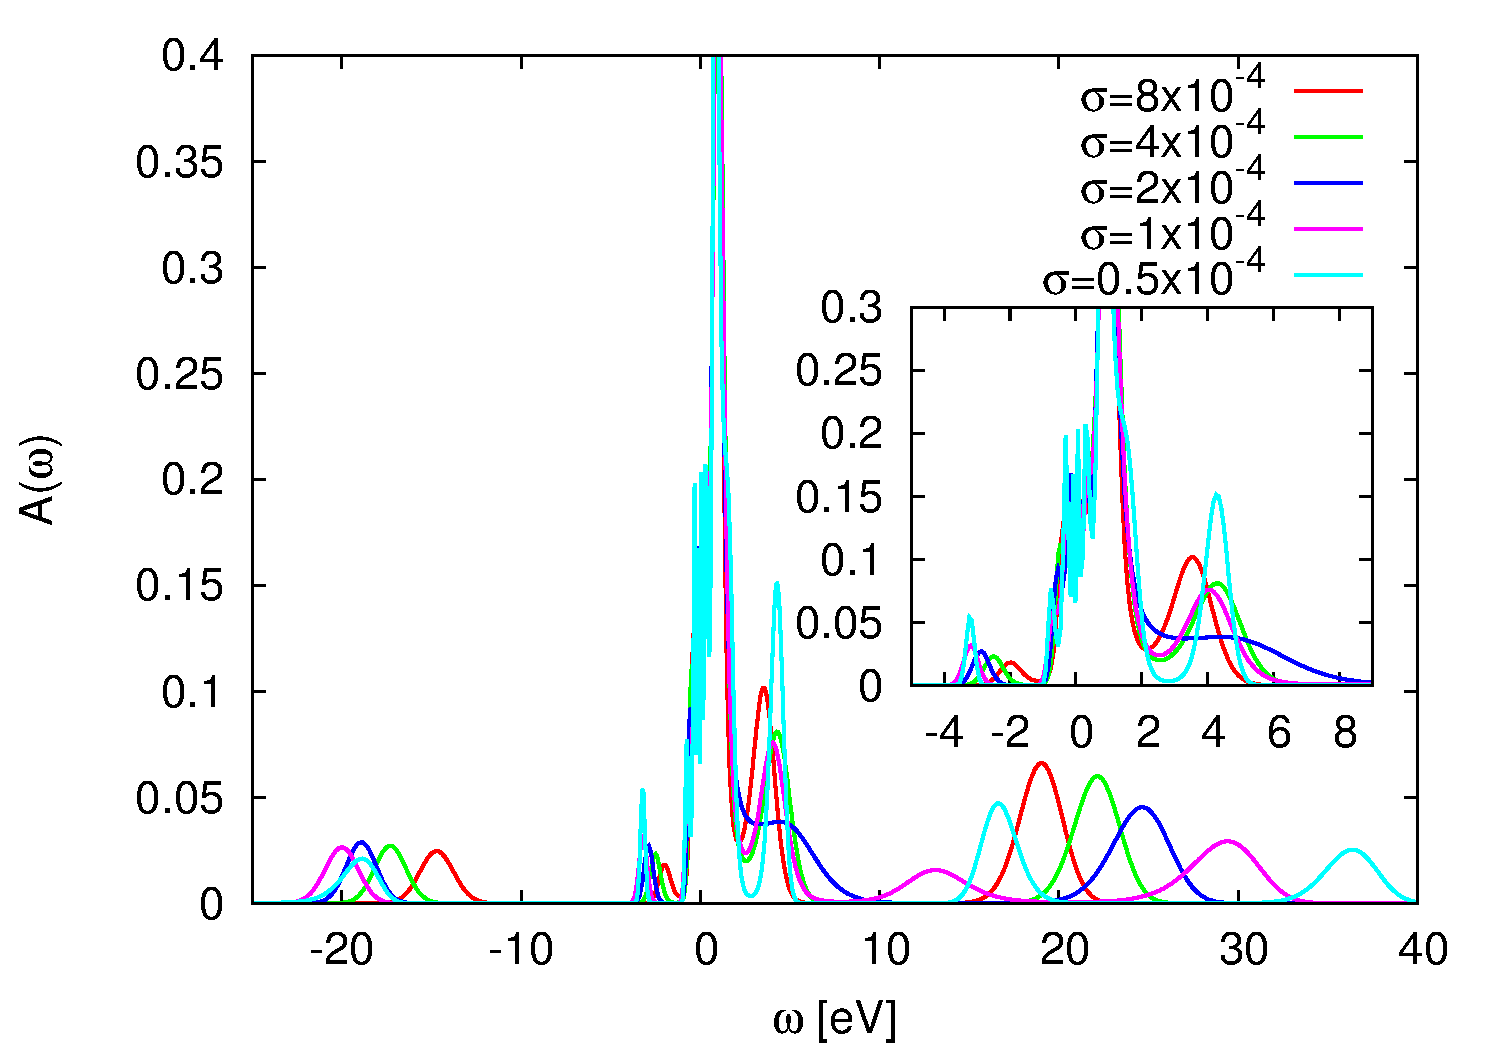
\includegraphics[width=0.75\textwidth]{figs/GW_maxent_diffSigma.pdf} 
\end{center}
\caption{The spectral function from G$_0$W$_0$ (7x7x7 k-points) obtained from
Maxent, using a constant standard deviation $\sigma$. The Green's function
on the Matsubara axis $i\omega_n$ for 1000 frequenices at $\beta=40$\ 1/eV was continued
using a gaussian default model.}
\label{fig:gw_anacont_diff_sigma}
\end{figure}

The analytic continuation becomes increasingly hard for the case
of frequency dependent interactions $U(\omega)$,
since plasmonic features appear in the spectral function, resp.
Green's function at multiples of the plasma frequency,
for example in SrVO$_3$ $\omega_p\approx 15$~eV.
Therefore, the energy window has to be chosen considerably large, at least $\pm 3\omega_p$
to obtain a proper normalization of the spectral function.

At the same time the high-energy features cannot be accurately resolved because the
kernel that has to be inverted becomes very small at high energies
\begin{align}
G(i\omega_n) &= \frac{1}{\pi} \int_{-\infty}^{\infty} \mathrm{Im}[G(\omega)] 
                                \frac{1}{\omega-i\omega_n}\mathrm{d}\omega \\
G(\tau) &= \frac{1}{\pi} \int_{-\infty}^{\infty} \mathrm{Im}[G(\omega)]
                             \frac{\mathrm{e}^{-\tau\omega}}{\mathrm{e}^{-\beta\omega}+1}\mathrm{d}\omega.
\end{align}
Performing the analytic continuation from the Matsubara axis $i\omega_n$
should in principle be easier, since the Kernel $K(\omega,i\omega_n)= \frac{1}{\omega-i\omega_n}$
does decay significantly slower than the Kernel
$K(\omega,\tau)=\frac{\mathrm{e}^{-\tau\omega}}{\mathrm{e}^{-\beta\omega}+1}$
for the continuation to the imaginary time axis $\tau$.
Therefore, plasmonic features at large $\omega$ are less suppressed
by $K(\omega,i\omega_n)$ than by $K(\omega,\tau)$, so small changes on the real
frequency axis $\omega$ should be more visible in $G(i\omega_n)$ than in $G(\tau)$.

In practice I think it is still better to use Maxent with $G(\tau)$
directly measured at $\tau_i$, since the Legendre representation usually used
on both $\tau$ and $i\omega_n$ introduces very spurious correlated errors
in the measured quantities, where no good error estimate exist.
Only for $G(\tau)$ we have a well defined measure of the error bar 
which is measured in the solver and should be used for the Maxent input. 
Maybe one can use the direct measurement on $i\omega_n$ (more costly)
in the future?

\begin{figure}[t]
\begin{center}
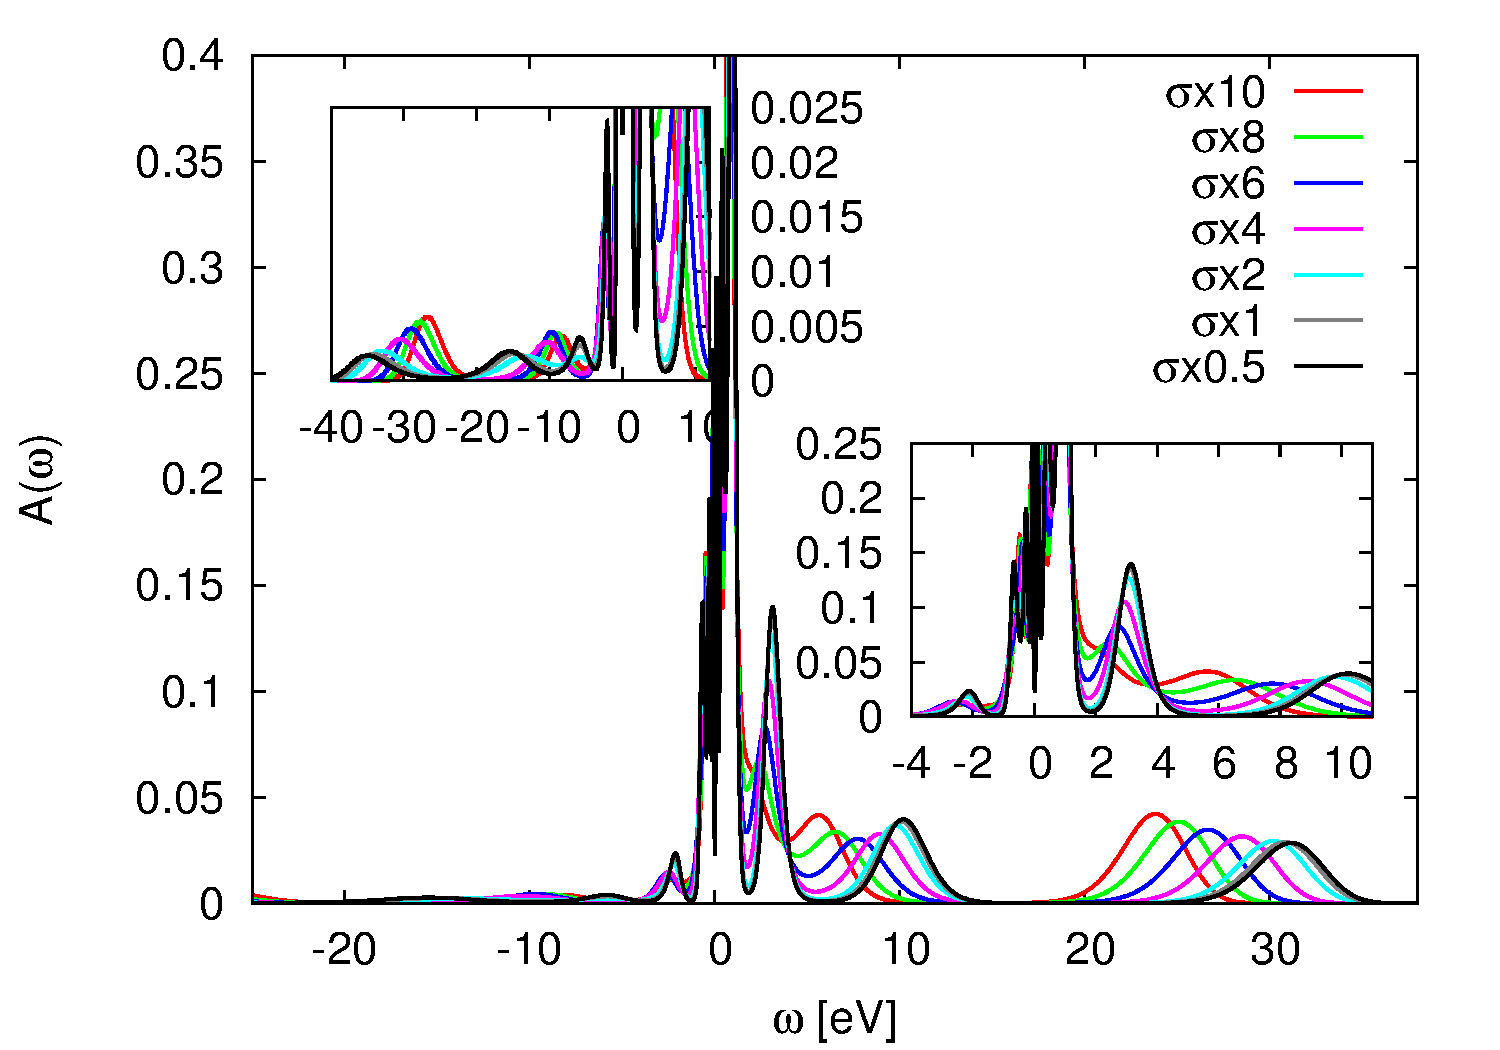
\includegraphics[width=0.75\textwidth]{figs/GWDMFT_maxent_diffSigma.pdf} 
\end{center}
\caption{The spectral function from GW+DMFT (7x7x7 k-points) obtained from
Maxent, using the mesured standard deviation $\sigma(\tau)$
from the impurity solver. The Green's function
on the imaginary time axis $\tau$ for 2048 points at $\beta=40$\ 1/eV was continued
using a gaussian default model. The standard deviation was scaled by different
factors to show the dependence on $\sigma$. The factor 1 corresponds
to the initial value of $\sigma$ measured in the Monte Carlo Solver.}
\label{fig:gwdmft_anacont_diff_sigma}
\end{figure}

\textbf{Essential tip:}
A very efficient way of dealing with the plasmonic weight at high frequencies
is by incorporating them already in the default model. What works quite well
is adding gaussians  at multiple of the plasma frequency 
$\pm n\omega_0$, with $n\sim 4$, that become smaller in weight.
Usually, the positions of these gaussians will not be modified becuase the 
analytic continuation is not sensitive enough to determine their correct position
but they are essential for redistributing spectral weight away from the Fermi level.
Another option is to add, instead of gaussians, only a constant value,
which reaches up to high energies. The important point here is that 
the spectral weight at the Fermi level, which is usually a bigger gaussian in
the default model, is properly reduced so that the analytic continuation
does not have to shift spectral weight from the Fermi level over long distances to higher
energies.

With both of these models, I noticed that the resulting spectral
function around the Fermi level is only very weakly dependent on the choice
of $\sigma$, which makes the result very robust and trustworthy.  
Also the position of the (first) upper and lower Hubbard bands seem to be 
quite robust. On both the imaginary time and frequency axis it worked quite well
and gave very similar results.



%%%%%%%%%%%%%%%%%%%%%%%%%%%%%%%%%%%%%%%%%%%%%%%%%%%%%%%%%%%%%%%%%%%%%%%%%%%%%%%%%%%%%
%%%%%%%%%%%%%%%%%%%%%%%%%%%%%%%%%%%%%%%%%%%%%%%%%%%%%%%%%%%%%%%%%%%%%%%%%%%%%%%%%%%%%
%%%%%%%%%%%%%%%%%%%%%%%%%%%%%%%%%%%%%%%%%%%%%%%%%%%%%%%%%%%%%%%%%%%%%%%%%%%%%%%%%%%%%
%%%%%%%%%%%%%%%%%%%%%%%%%%%%%%%%%%%%%%%%%%%%%%%%%%%%%%%%%%%%%%%%%%%%%%%%%%%%%%%%%%%%%
%%%%%%%%%%%%%%%%%%%%%%%%%%%%%%%%%%%%%%%%%%%%%%%%%%%%%%%%%%%%%%%%%%%%%%%%%%%%%%%%%%%%%
\clearpage

\section{Dependence on the k-mesh}

This section discusses the sensitivity of the GW calculation on the number of
k-points. There are three quantities of interest:\\
The Kohn-Sham DFT Hamiltonian $H_{DFT}$, the exchange-correlation
potential $V_{XC}$  and the GW Selfenergy $\Sigma^{GW}_{XC}$.
All of them are given in the Basis of Wannier orbitals.

In general the GW calculation is limited to k-meshes with a size from
$5\times 5\times 5$ to maximum $10\times 10\times 10$, depending on how large the system
is. Currently the limitation of the GW calculation is the memory and disk space.
For example a $8\times 8\times 8$ calculation for SrVO$_3$ exceeds the 128Gbyte
RAM on a single node on Hedin and uses more than 1Tbyte of disk space.
The computation time is still manageable with less than one week.

After the GW calculation the result is interpolated to a very dense k-mesh
by a 3D cubic interpolation scheme, which so far has been very reliable.

\clearpage

\subsection{SrVO$_3$}

\begin{figure}[h]
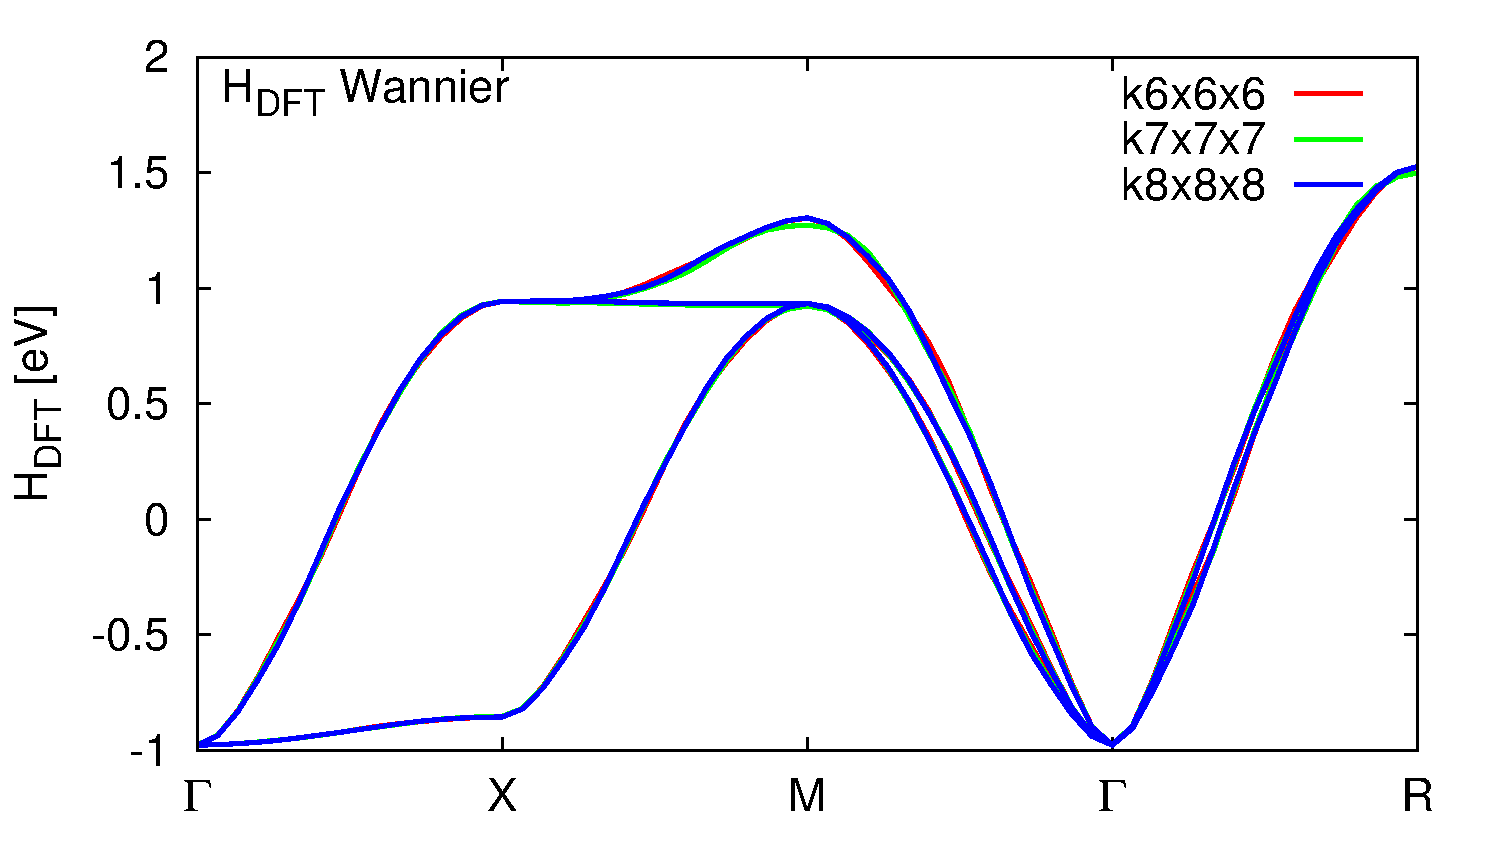
\includegraphics[width=0.5\textwidth]{figs/kmesh/hdft_kpath.pdf}
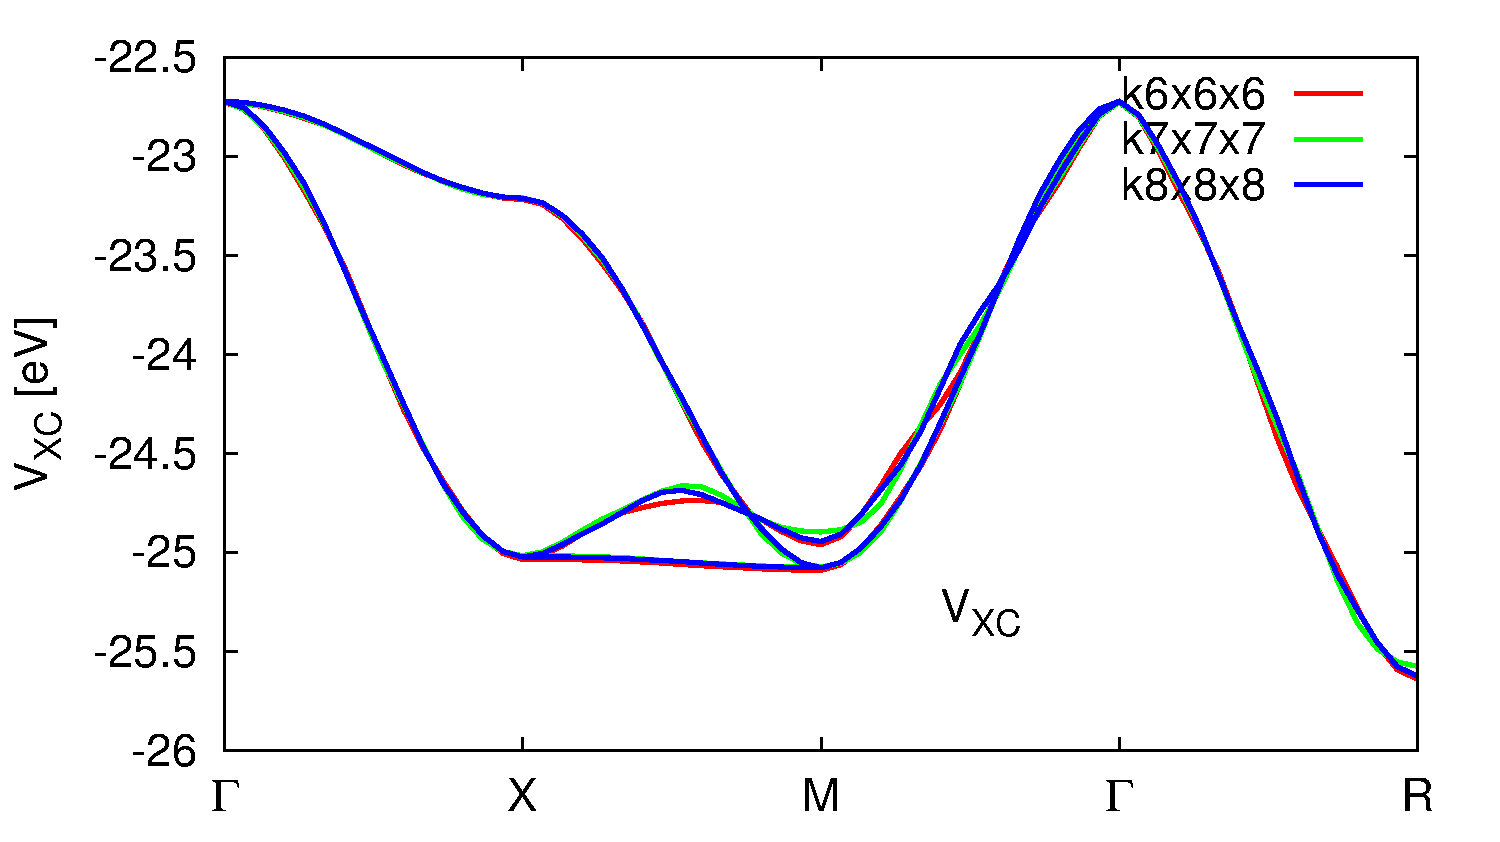
\includegraphics[width=0.5\textwidth]{figs/kmesh/vxc_kpath.pdf}
\begin{center}
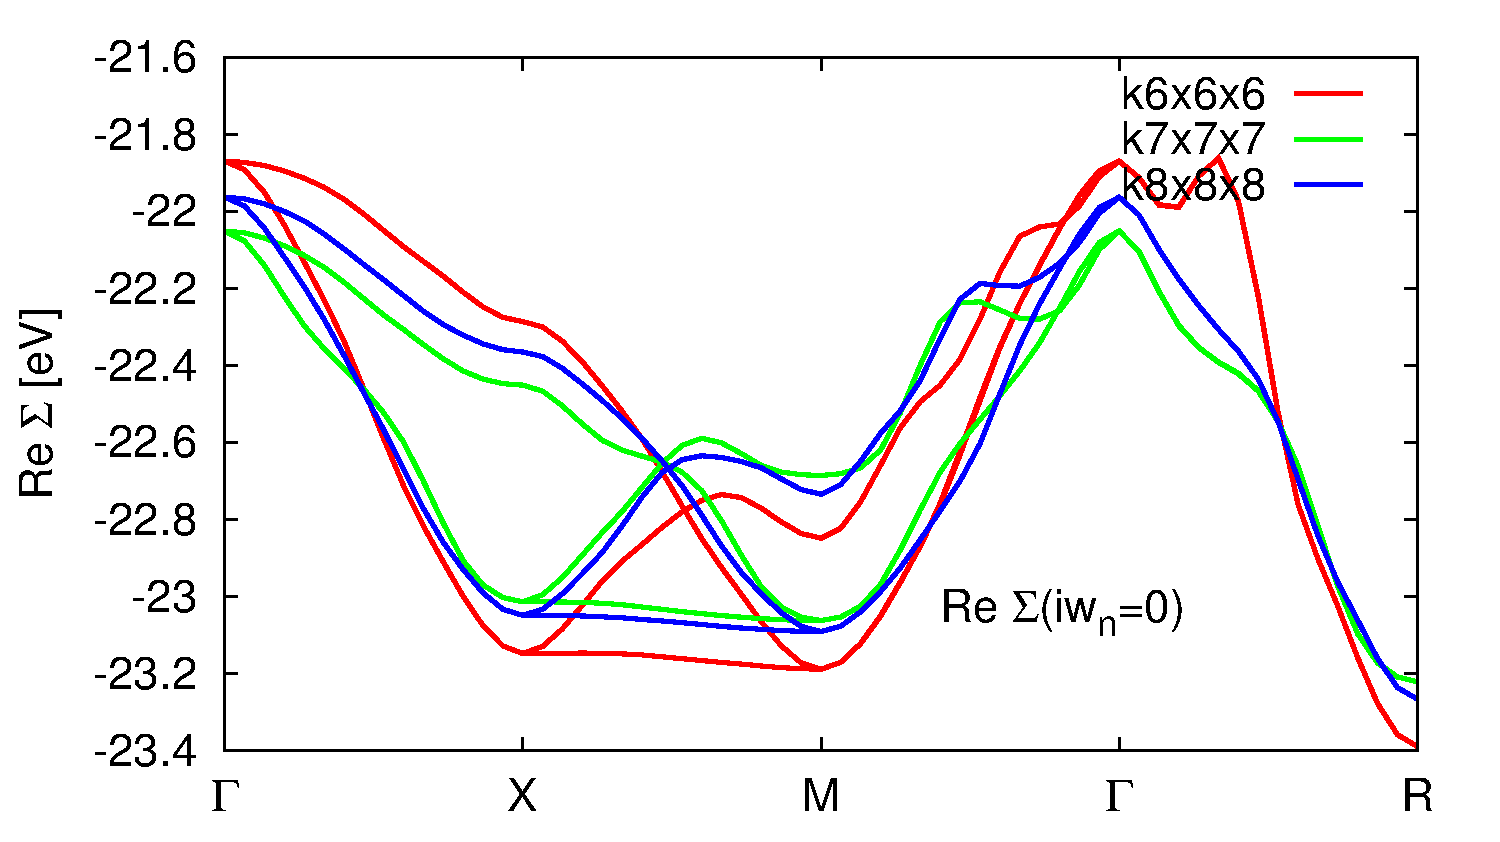
\includegraphics[width=0.7\textwidth]{figs/kmesh/ReSigma_kpath.pdf}
\end{center}
\caption{
These plots show a comparison of the convergence of $H_{DFT}$, $V_{XC}$ and
$\Sigma^{GW}_{XC}$ in the Wannier basis as a function of number of k-points for SrVO$_3$.\\
Top Left: The Eigenvalues of the DFT tight-binding Hamiltonian $H_{DFT}$.\\
Top Right: The exchange-correlation potential $V_{XC}$. \\
Bottom: The real part of the \textbf{local} $G_0W_0$ Selfenergy, which is equal for 
all 3 $t_{2g}$ orbitals, evaluated at the lowest Matsubara frequency ($\beta=40$\ 1/eV). }
\label{fig:gw_kpath_kmesh_comp}
\end{figure}


In Fig. \ref{fig:gw_kpath_kmesh_comp} we show 
the Eigenvalues of the DFT tight-binding Hamiltonian $H_{DFT}$,
the exchange-correlation potential $V_{XC}$ and the real part of the $G_0W_0$ 
Selfenergy at the lowest Matsubara frequency at $\beta=40$\ 1/eV
along a certain k-path. Calculations based on different k-meshes in the GW calculation
are compared.
All objects have been interpolated to a $30\times30\times30$ k-mesh.

$H_{DFT}$ shows basically negligible variation for different number of k-points 
since the values are directly taken from the DFT calculation converged on a much denser grid.
The only variation is due to the interpolation from the smaller to the larger grid,
which becomes more accurate  with higher number of k-points.

Interestingly, $V_{XC}$ shows a much larger variation than $H_{DFT}$, for example of up 
to $50$~meV along the X-M direction. Since for all calculations $V_{XC}$ in the Kohn-Sham
space is identical, this indicates that $V_{XC}$ is either more difficult to interpolate
because it is less smooth than $H_{DFT}$, or that it is itself
more sensitive to the accuracy of the Wannier orbitals, which becomes more accurate
with larger k-meshes.
 
The GW Selfenergy $\Sigma^{GW}_{XC}$ shows a really strong variation with different k-meshes
and still changes more than 100meV at some k-points when increasing the mesh
from $7\times 7 \times 7$ to $8\times 8 \times 8$.
These changes of the "bandwidth" that can be seen in the plot directly amount to a different 
renormalization due to the GW selfenergy, which will later have an effect
on the GW+DMFT cycle.

\bigskip

\textbf{Plan: I think I would be satisfied with a $9\times 9  \times 9$
calculation. This might be possible if I can get $\sim$900 cores on Hedin for maybe a week...}



\clearpage

\subsection{FeSe}

\begin{figure}[h]
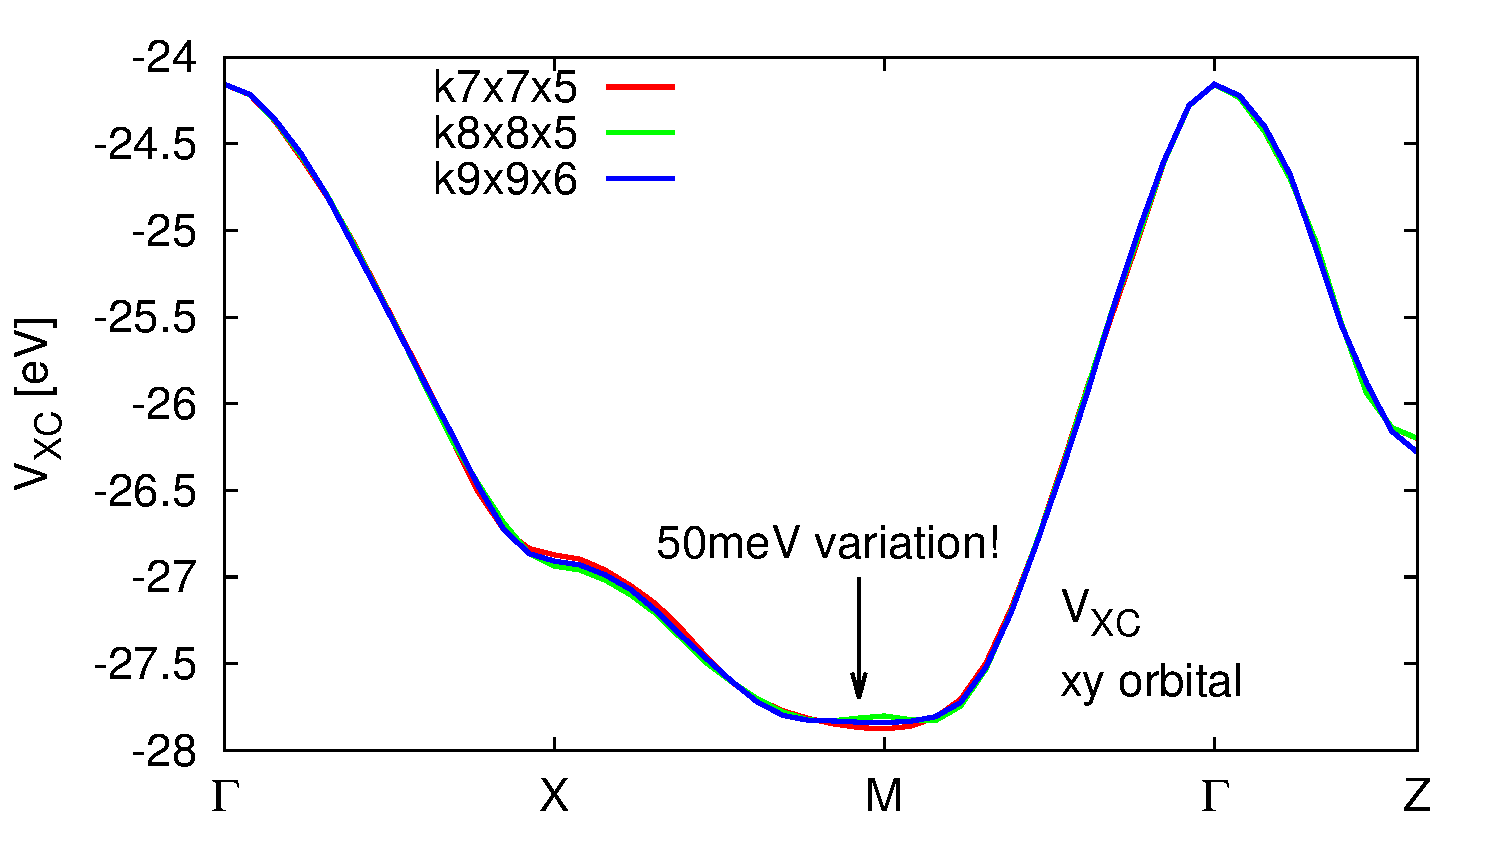
\includegraphics[width=0.5\textwidth]{figs/kmesh/FeSe/vxc_kpath_xy.pdf}
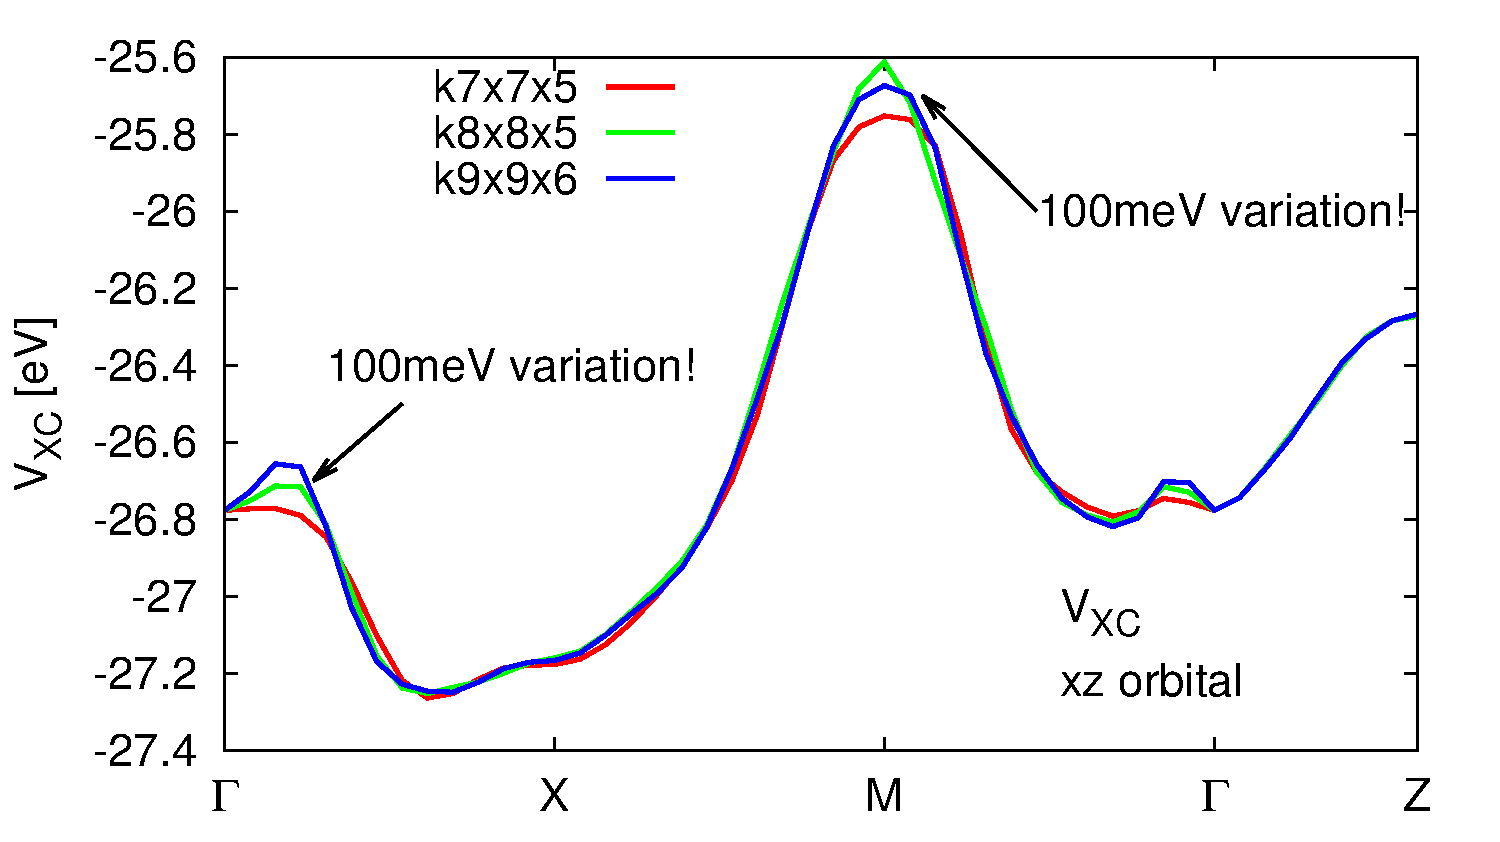
\includegraphics[width=0.5\textwidth]{figs/kmesh/FeSe/vxc_kpath_xz.pdf}
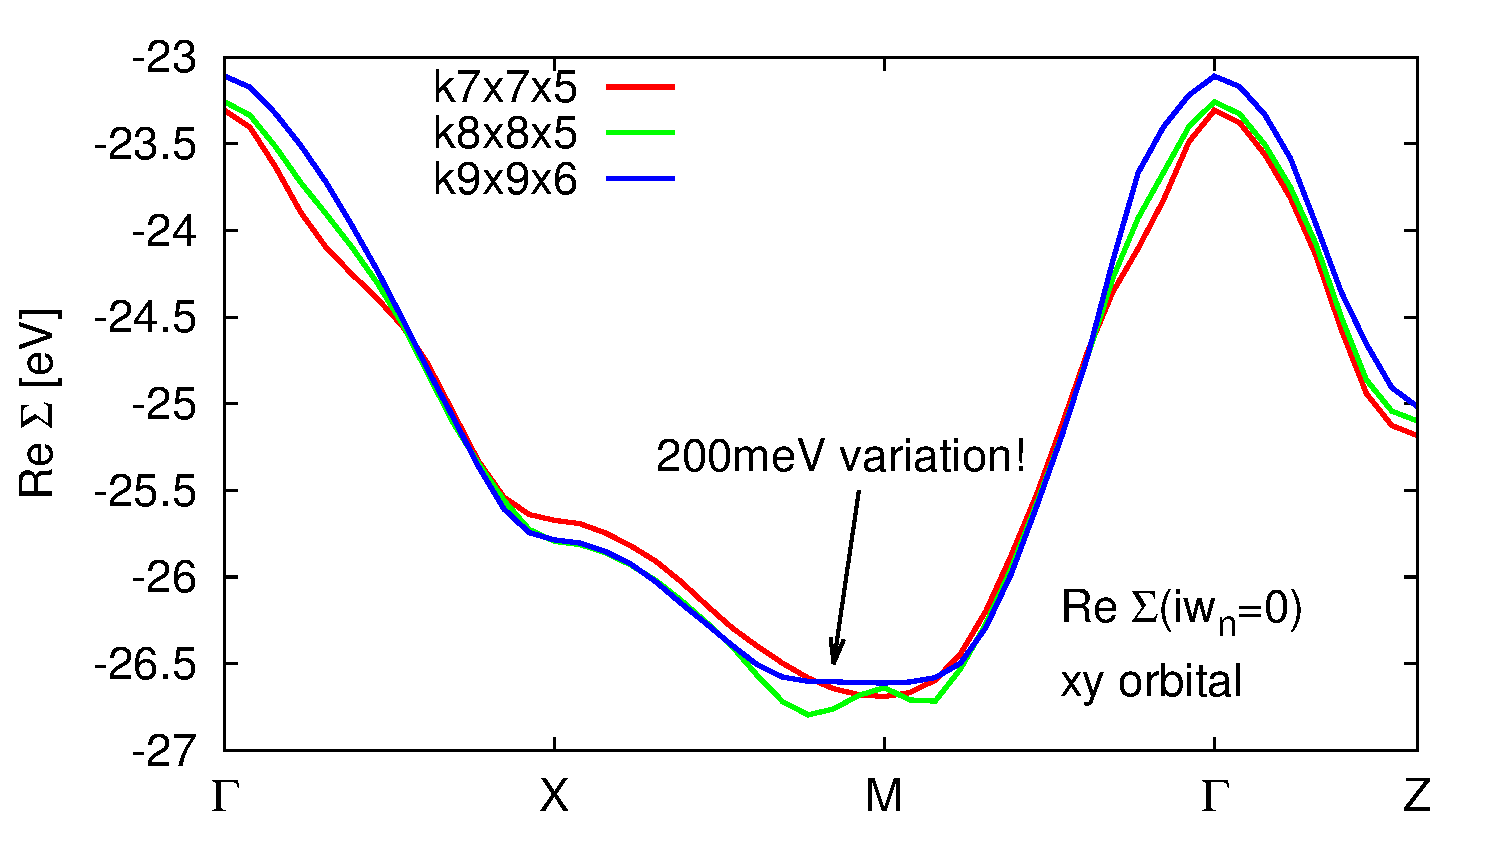
\includegraphics[width=0.5\textwidth]{figs/kmesh/FeSe/ReSigma_kpath_xy.pdf}
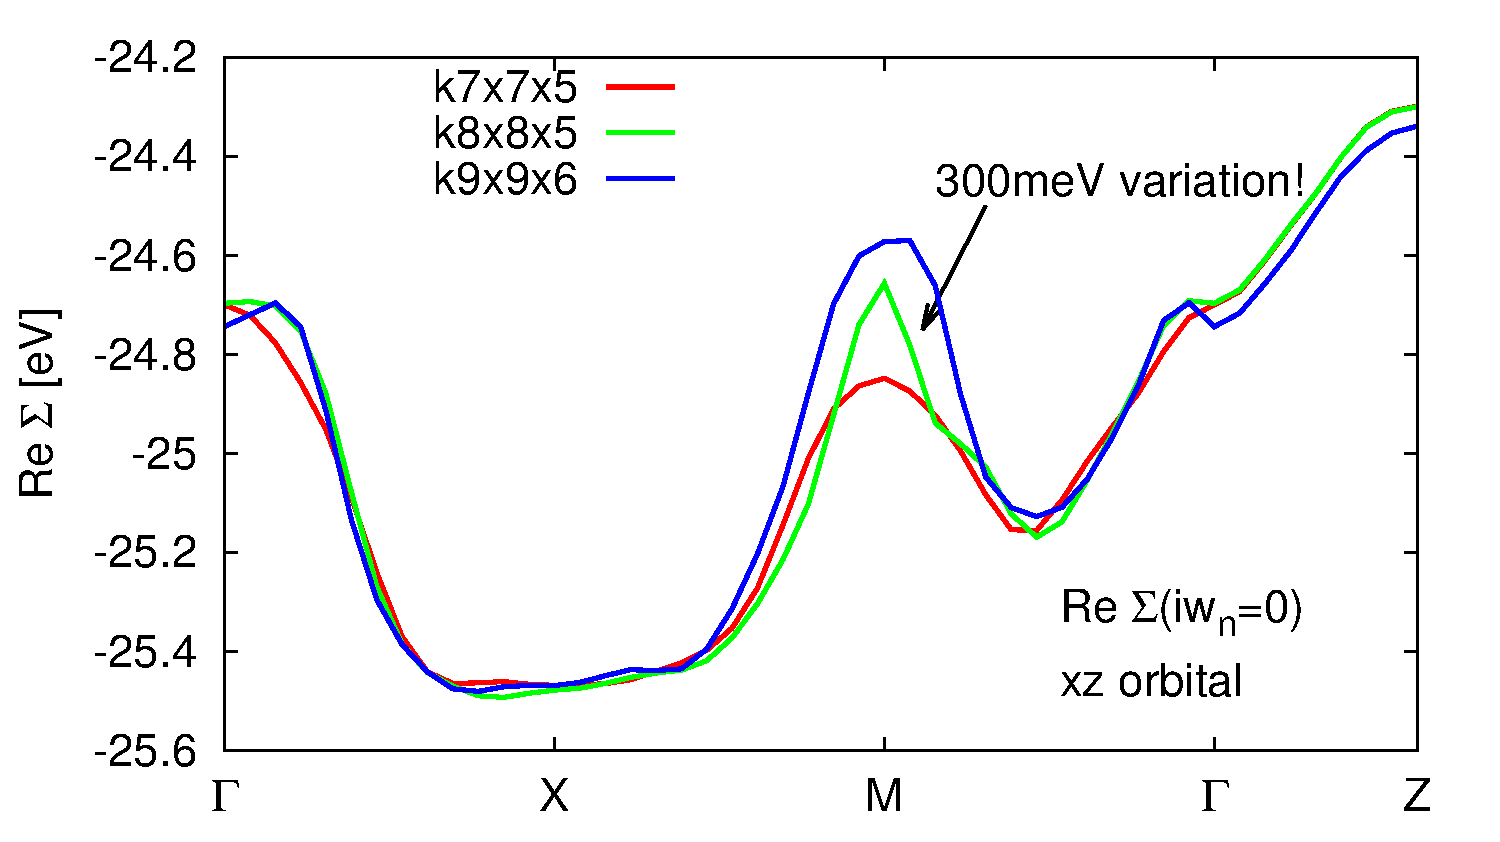
\includegraphics[width=0.5\textwidth]{figs/kmesh/FeSe/ReSigma_kpath_xz.pdf}
\caption{Top: The exchange-correlation potential $V_{XC}$
for the 3dxy and 3dxz orbital for FeSe \\
Bottom: The real part of the $G_0W_0$ Selfenergy at the lowest Matsubara frequency
for the 3dxy and 3dxz orbital. }
\label{fig:FeSe_kpath_kmesh_comp}
\end{figure}

Here we compare the exchange correlation potential and the GW Selfenergy
for FeSe. The Kohn-Sham Hamiltonian was basically identical for all
k-meshes, so we do not show it here.

Fig.~\ref{fig:FeSe_kpath_kmesh_comp} shows $V_{XC}$ and $\Sigma^{GW}_{XC}$ again
along a certain k-path.
The variations are a bit larger compared to SrVO$_3$, especially around
the M point one can observe artefacts. Especially the Selfenergy
varies dramatically in the 3dxz orbital, with variation of about $300$~meV.
These variations directly translate to shifts of "bands", also around the Fermi
level. 
This can be seen clearly when calculating the full
GW spectral function, shown in Fig.~\ref{fig:FeSe_GW_spec_comp}.
There are artefacts appearing basically at all high-symmetry points,
but especially severe around the M point.
In this case the $9\times 9\times 6 $ mesh fixes these problems, but 
even this mesh cannot be considered to be converged sufficiently.

Interestingly, the calculations with odd number of k-points
along each axis seem to show less artefacts, probably because the
high-symmetry points are excluded and obtained only by interpolation.

\textbf{Plan: I think I would be satisfied with a $9\times 9  \times 7$
calculation. This is currently running...}

\begin{figure}[h]
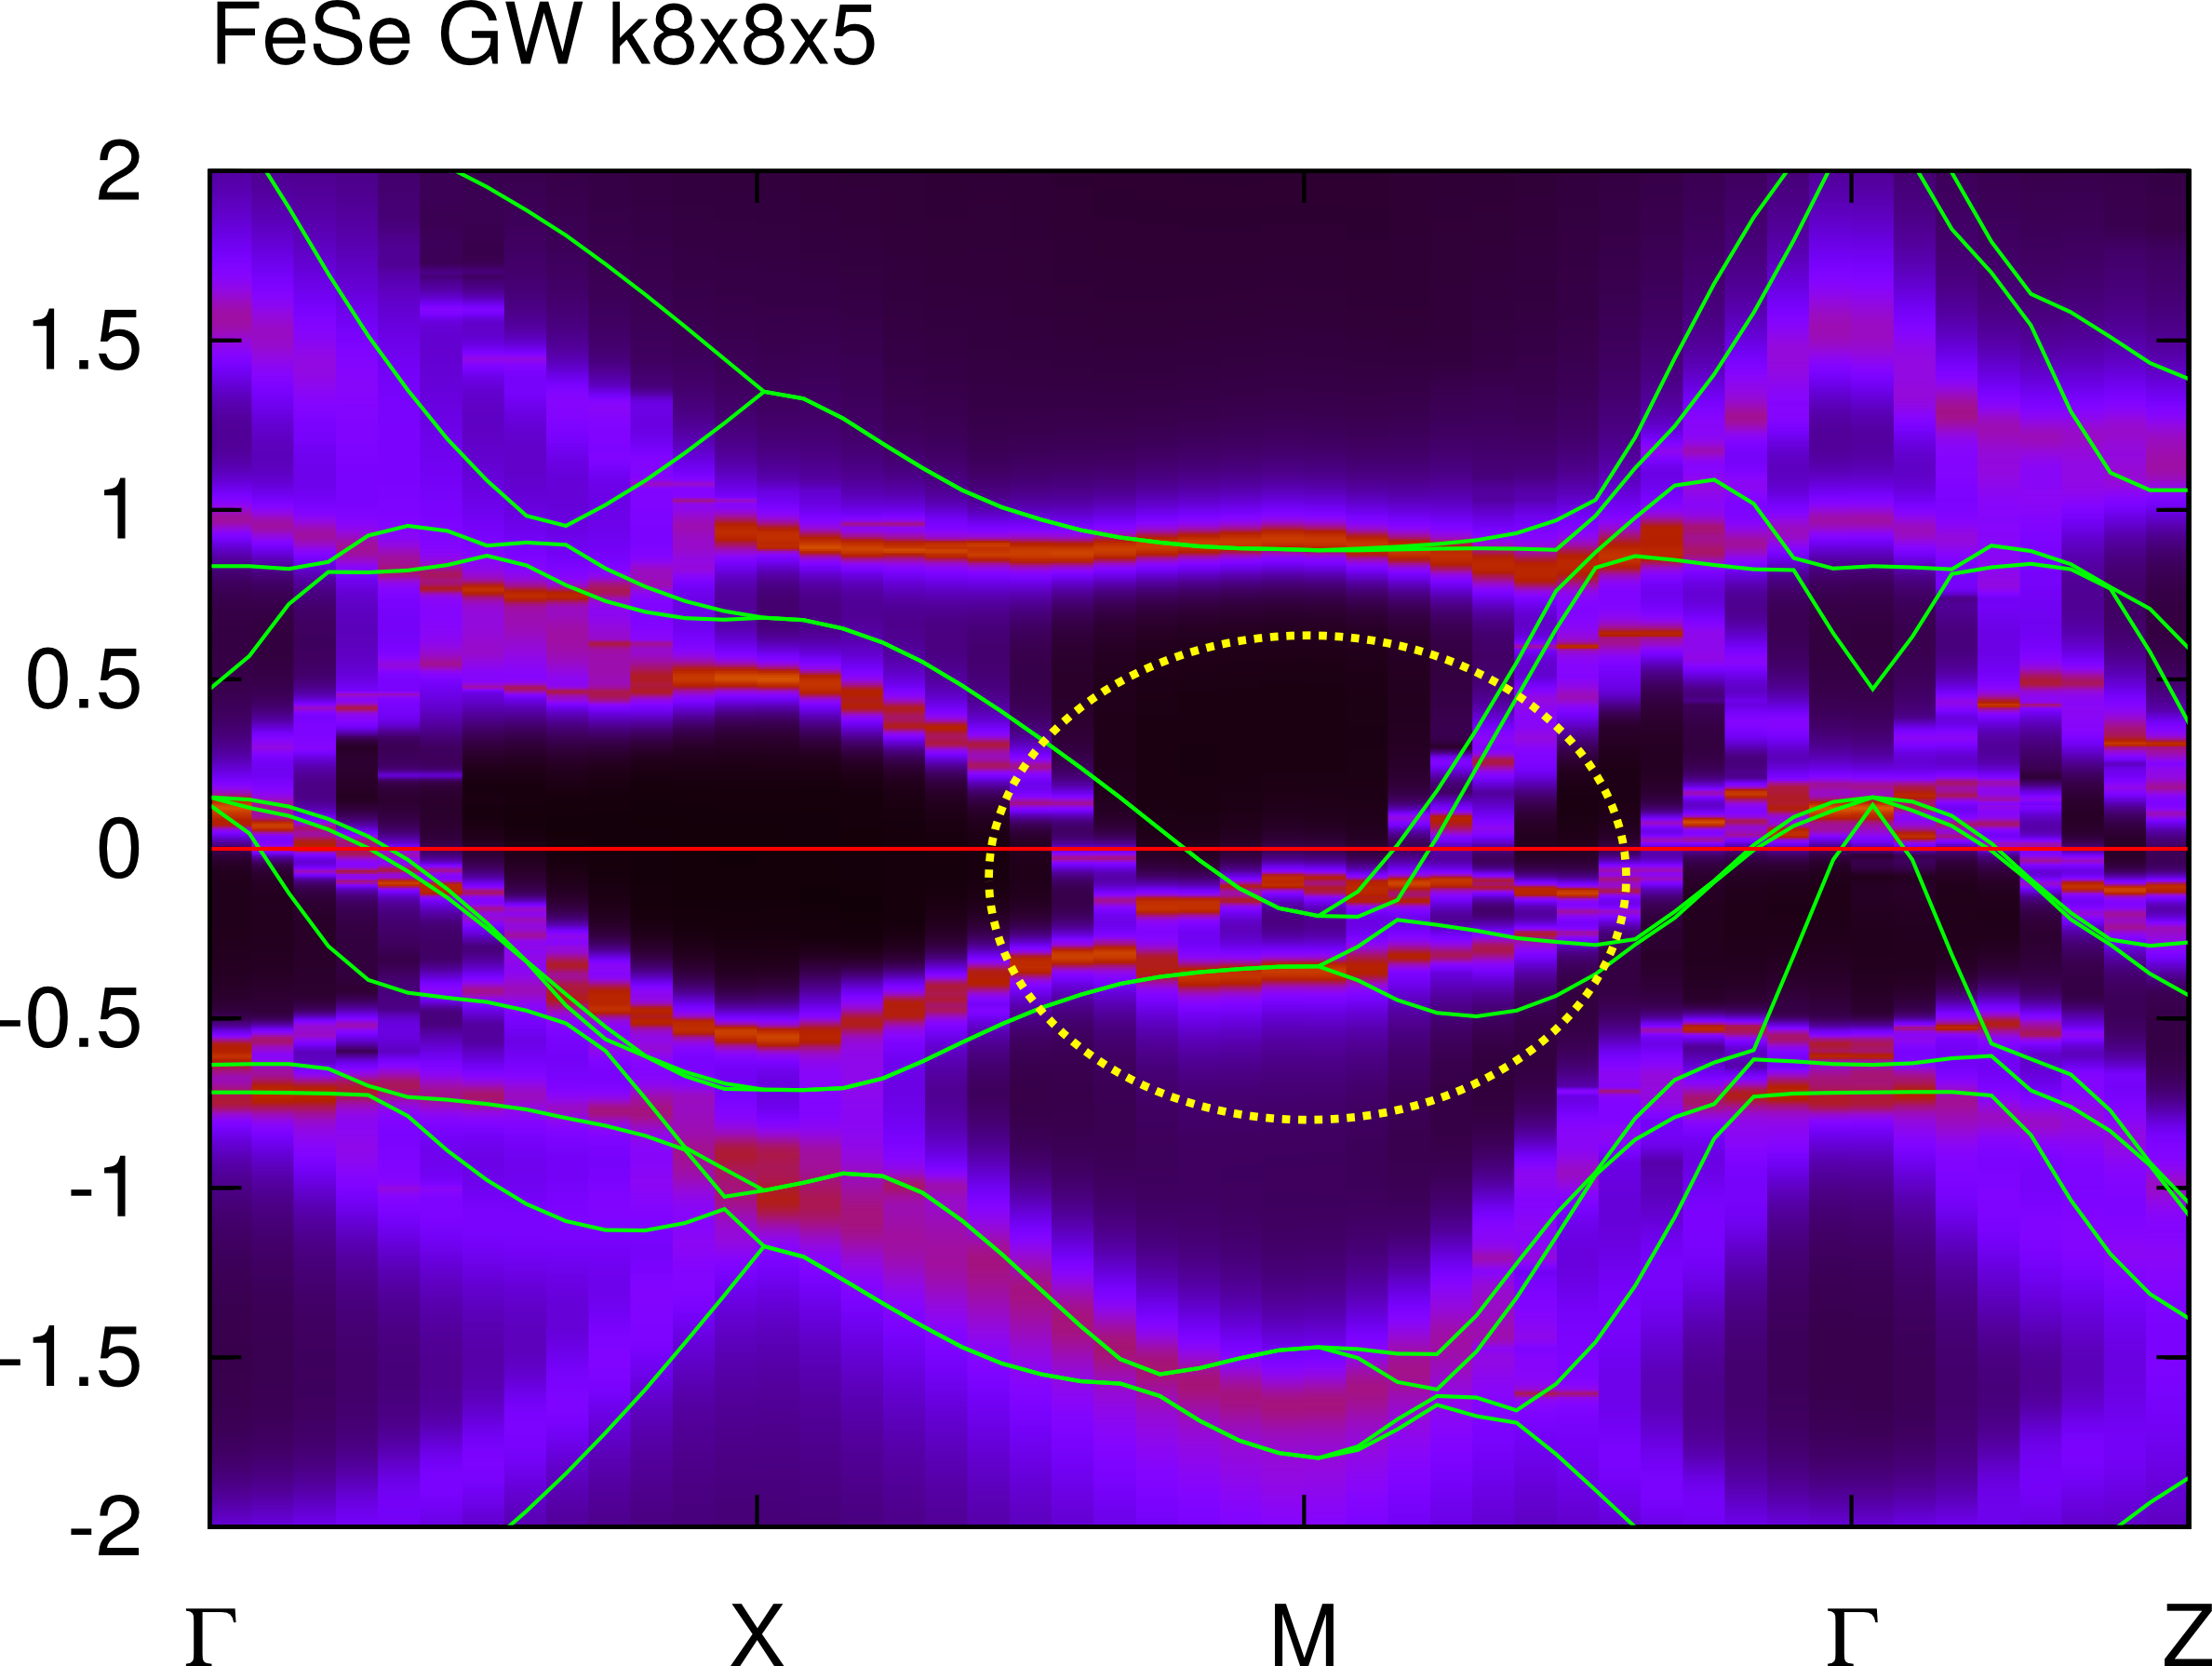
\includegraphics[width=0.9\textwidth]{figs/kmesh/FeSe/FeSe_bands_GW_k885.png}
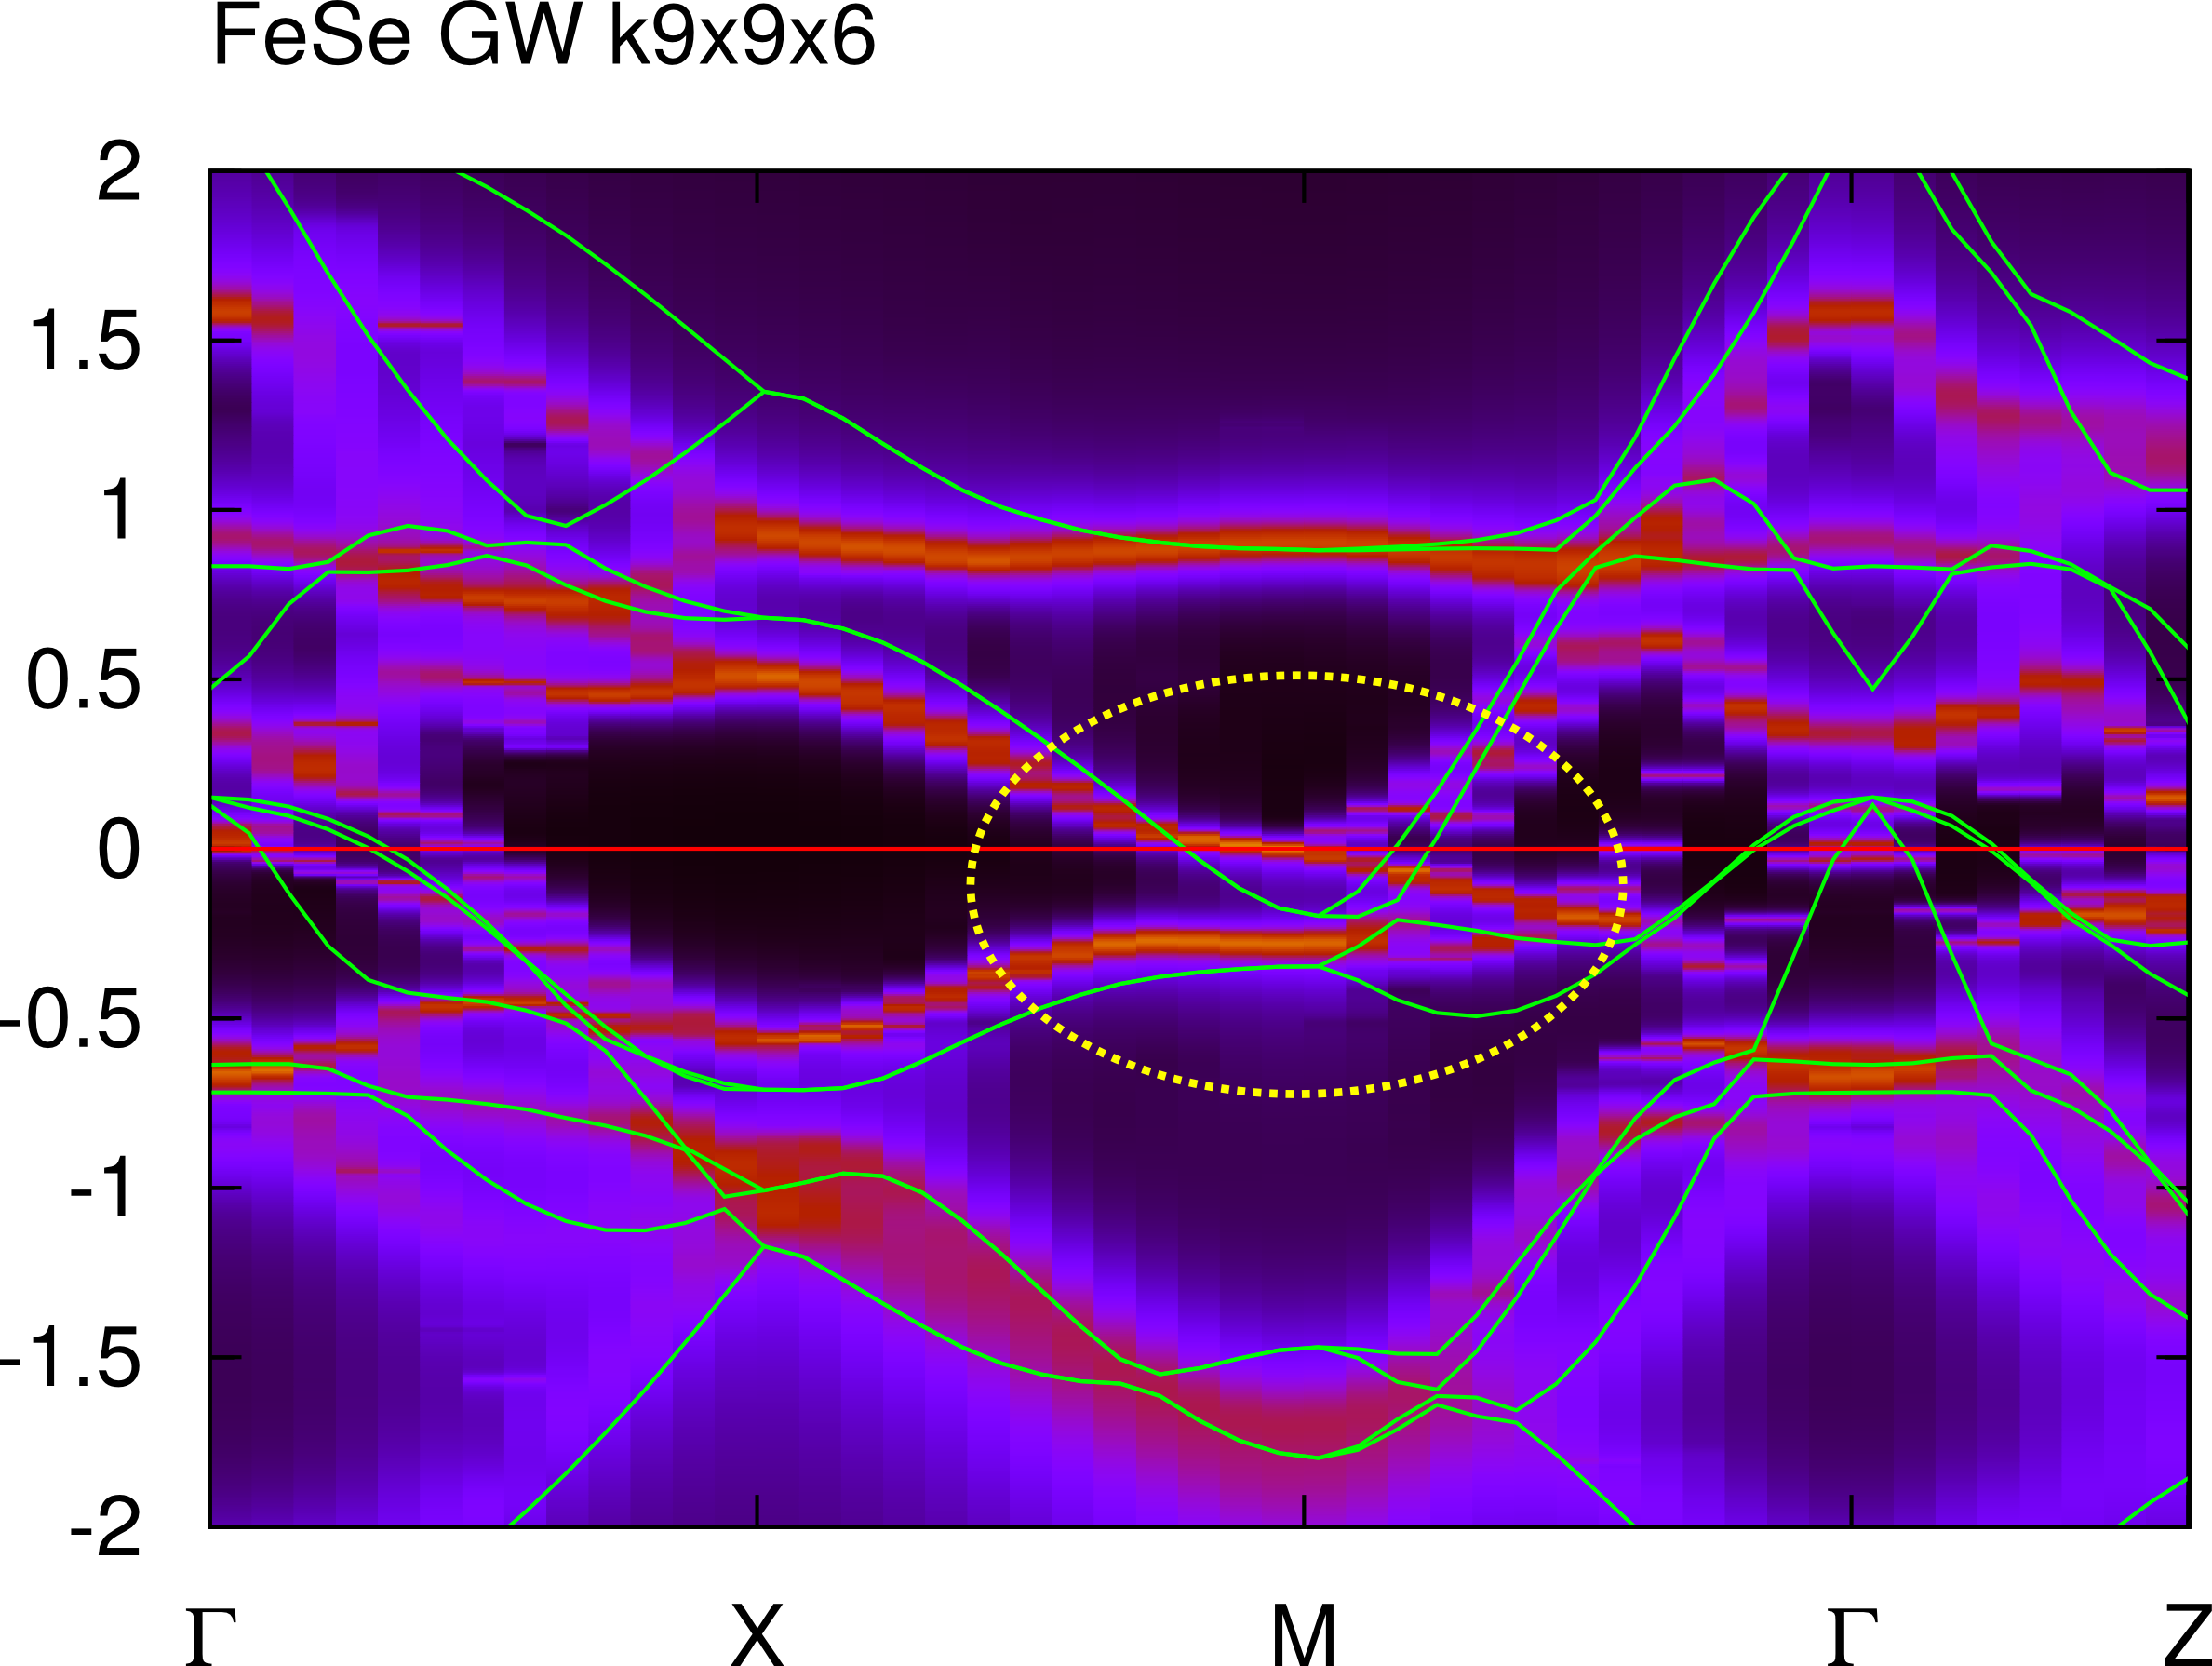
\includegraphics[width=0.9\textwidth]{figs/kmesh/FeSe/FeSe_bands_GW_k996.png}

\caption{The spectral function of FeSe calculated within GW. Upper panel
shows the result for a $8\times 8\times 5$ k-mesh,
and the lower one for a $9\times 9\times 6$ k-mesh. 
The green lines are the DFT result. The artefacts at the M point (yellow circle)
are a result of the k-mesh being still too coarse.}
\label{fig:FeSe_GW_spec_comp}
\end{figure}

\clearpage

%%%%%%%%%%%%%%%%%%%%%%%%%%%%%%%%%%%%%%%%%%%%%%%%%%%%%%%%%%%%%%%%%%%%%%%%%%%%%%%%%%%%%
%%%%%%%%%%%%%%%%%%%%%%%%%%%%%%%%%%%%%%%%%%%%%%%%%%%%%%%%%%%%%%%%%%%%%%%%%%%%%%%%%%%%%
%%%%%%%%%%%%%%%%%%%%%%%%%%%%%%%%%%%%%%%%%%%%%%%%%%%%%%%%%%%%%%%%%%%%%%%%%%%%%%%%%%%%%
%%%%%%%%%%%%%%%%%%%%%%%%%%%%%%%%%%%%%%%%%%%%%%%%%%%%%%%%%%%%%%%%%%%%%%%%%%%%%%%%%%%%%
%%%%%%%%%%%%%%%%%%%%%%%%%%%%%%%%%%%%%%%%%%%%%%%%%%%%%%%%%%%%%%%%%%%%%%%%%%%%%%%%%%%%%

\section{Dependence on GW frequency mesh}
\begin{figure}[h]
\begin{center}
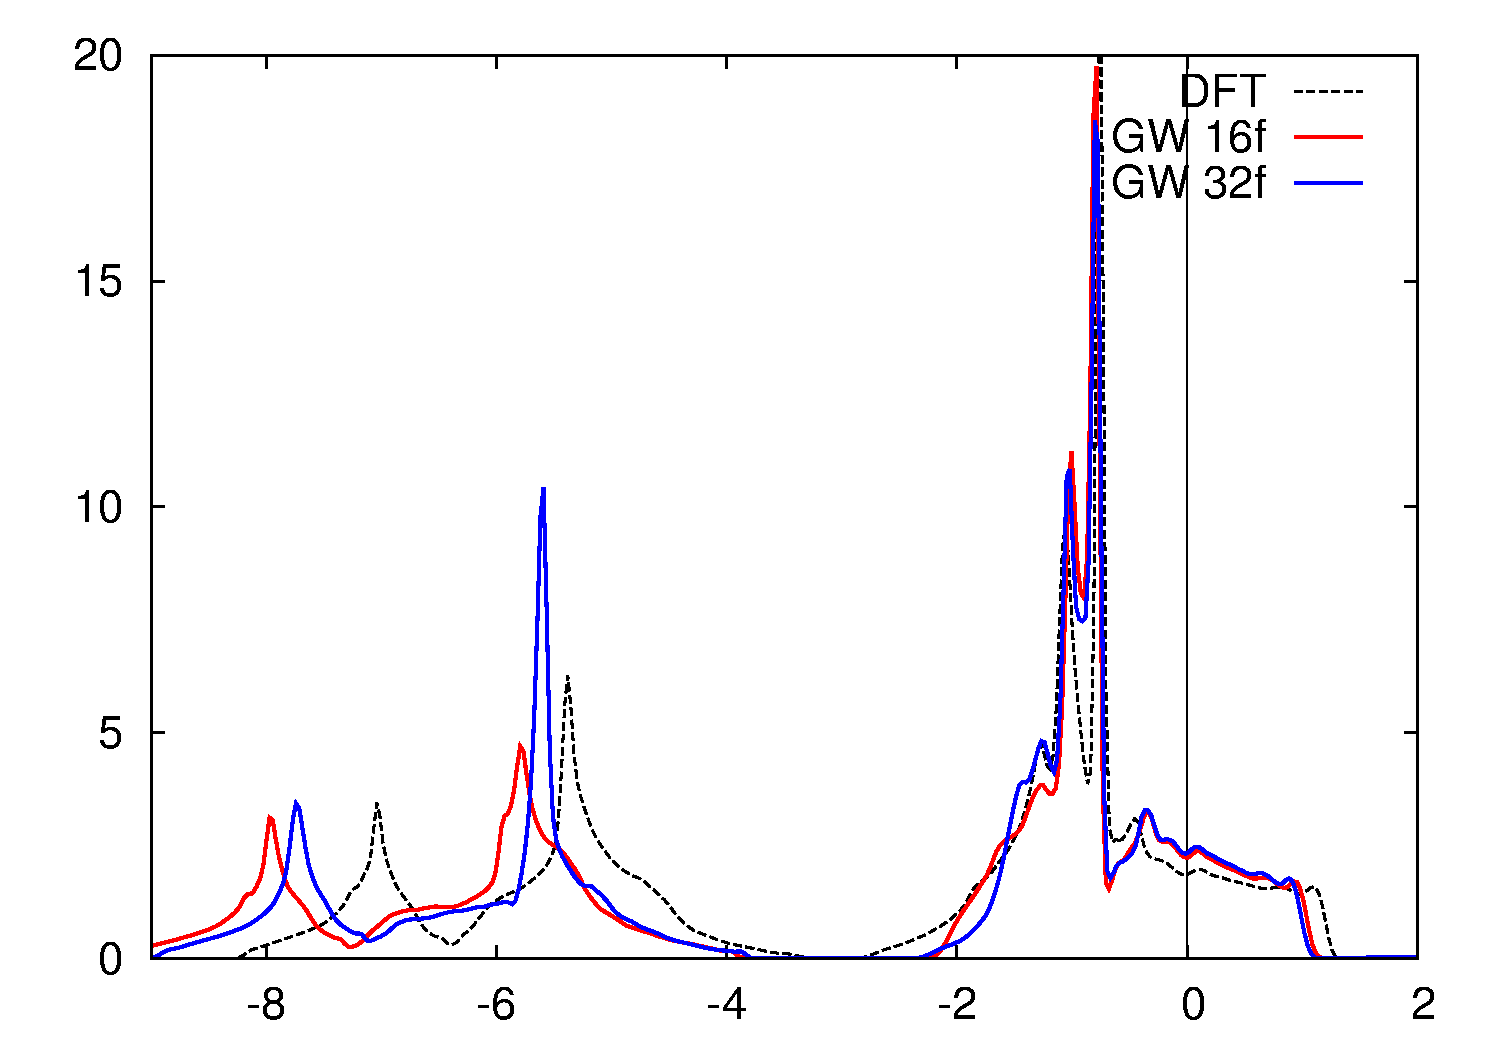
\includegraphics[width=0.6\textwidth]{figs/freqdep/NiO_fcomp_DOS.pdf} 
\end{center}
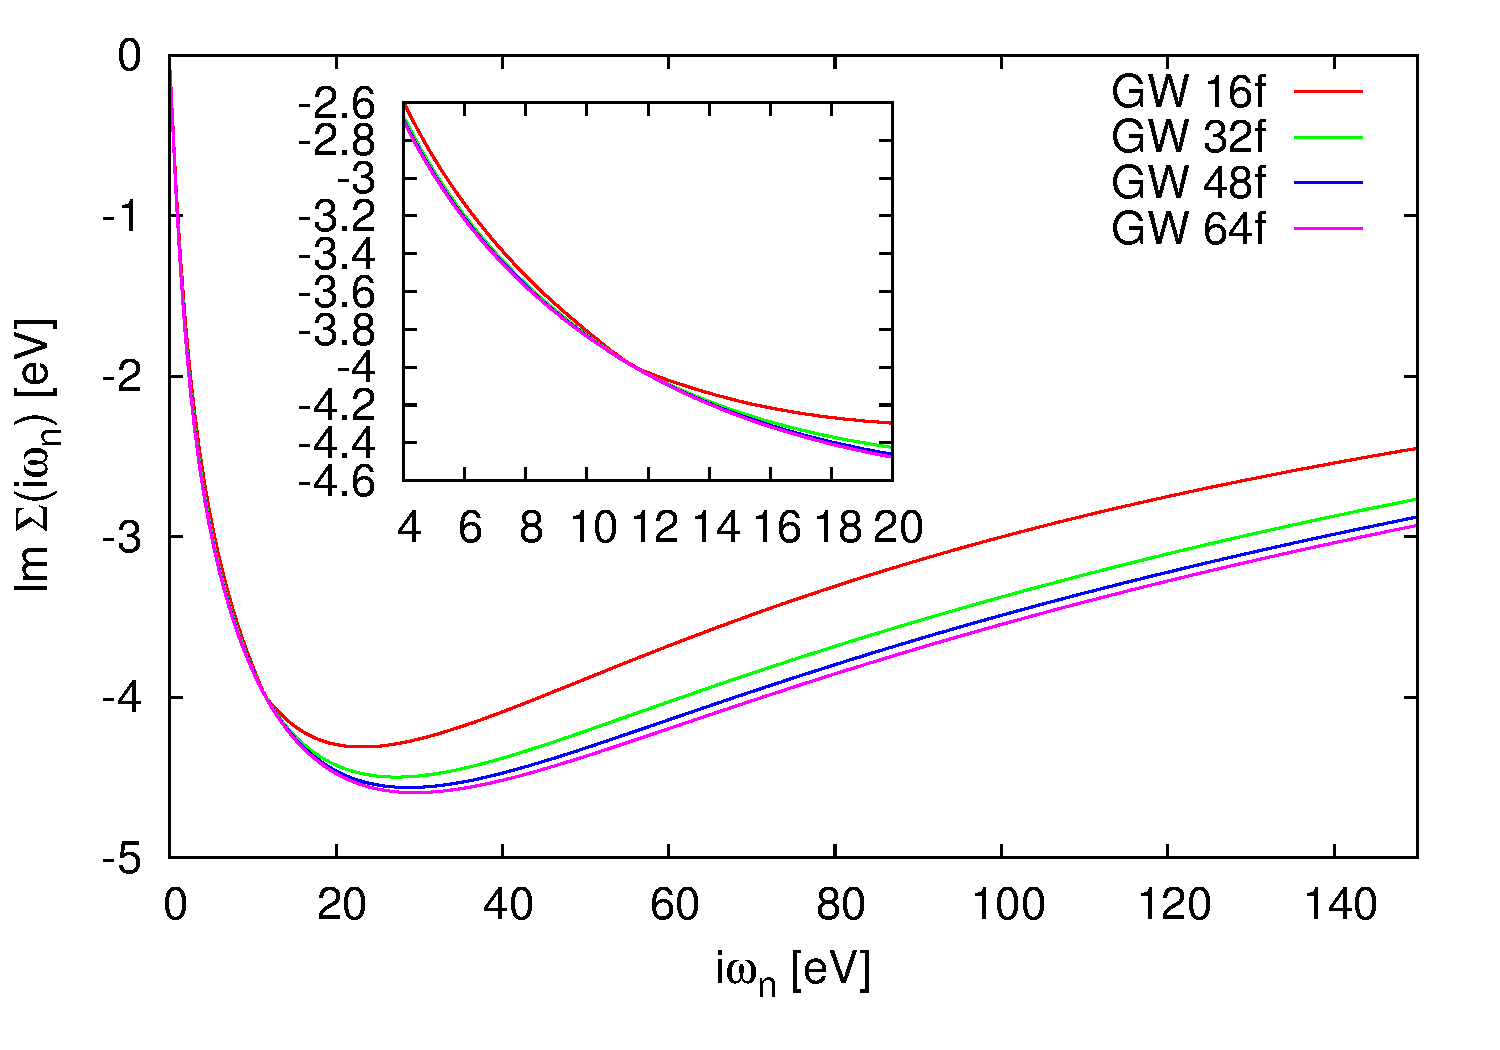
\includegraphics[width=0.49\textwidth]{figs/freqdep/NiO_fcomp_sigmai.pdf}
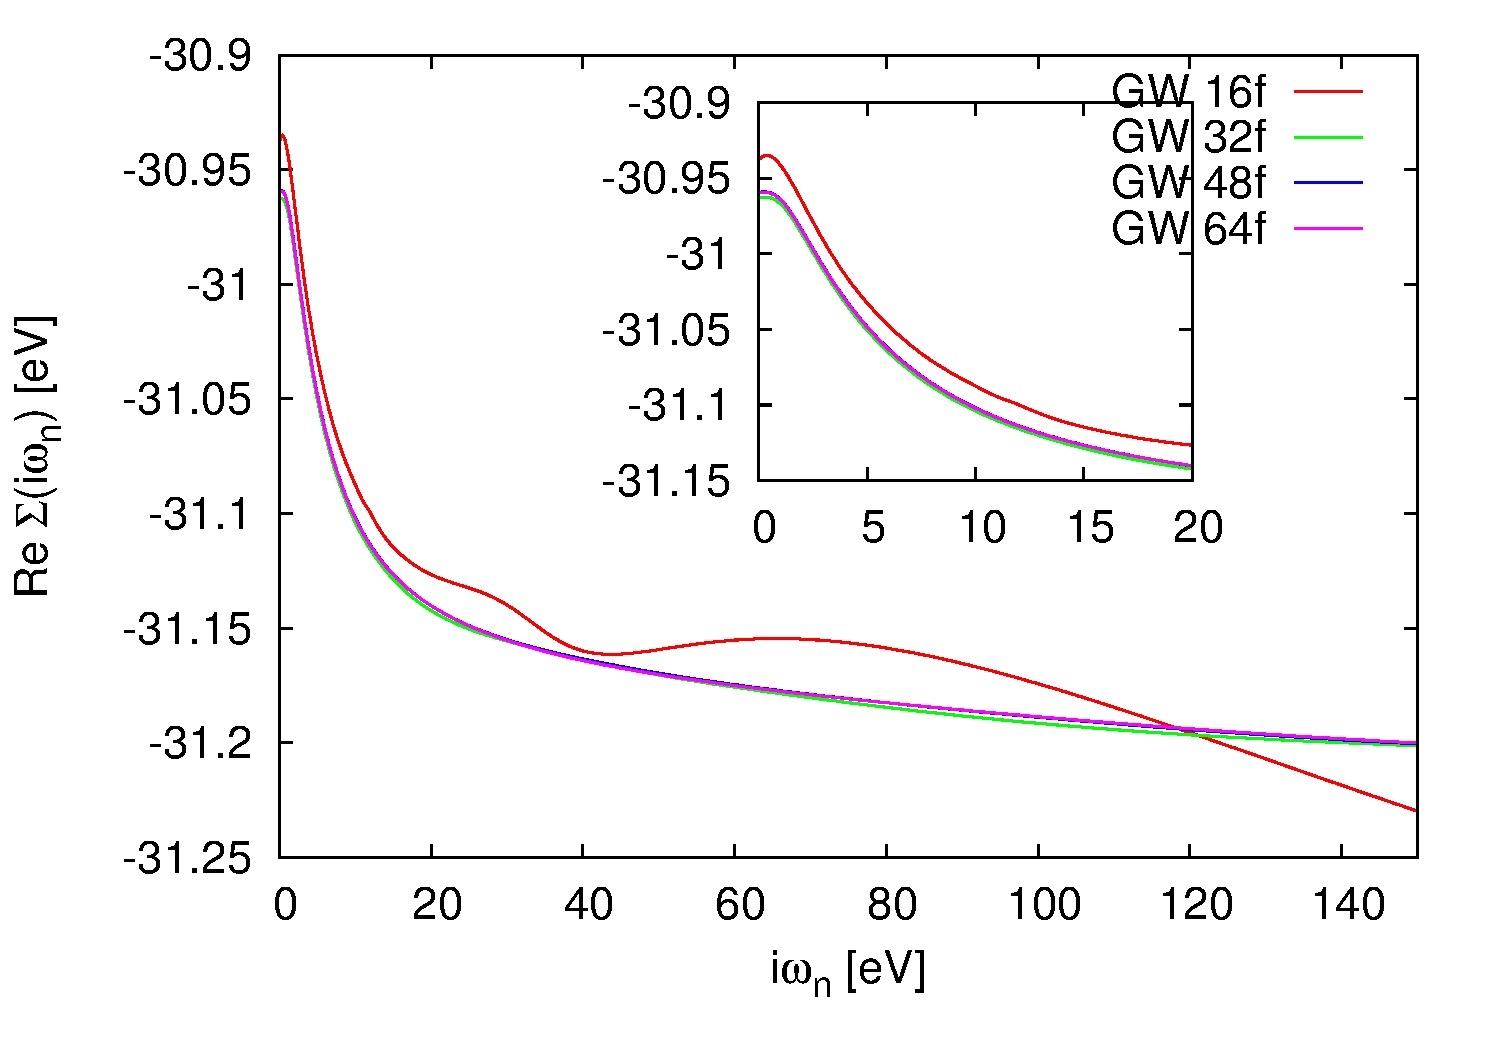
\includegraphics[width=0.49\textwidth]{figs/freqdep/NiO_fcomp_sigmar.pdf}
\caption{Top: The GW quasiparticle DOS for NiO with different number of
frequenices used for sampling the Polarization/Selfenergy.
Bottom: The resulting selfenergy for different number of frequencies. In the imaginary
part the Selfenergy at the Gamma point for the $e_g$ orbitals is shown, while
in the real part it is shown at the X point for the first $e_g$ orbital.}
\label{fig:gw_freqdep_comp}
\end{figure}

In the GW Code the frequency dependent objects are stored on a specific
frequency mesh, which is also used for integration when evaluating the 
Selfenergy 
\begin{align}
 \Sigma^{GW}(i\omega) &= \int \mathrm{d}{i\nu}\ G(i\omega-i\nu) W(i\nu).
\end{align}

In the gw.inp input file one has the parameters
\begin{description}
\item[iop\_fgrid]:
\begin{description}
 \item[1] Equally spaced mesh
 \item[2] single Gauss-Laguerre quadrature
 \item[3] Double Gauss-Legendre quadrature from 0 to omegmax and from omegmax to infinity
 \item[4] Fermion Matsubara frequencies
\end{description}
The default is the double Gauss-Legendre quadrature, in which the semi-infinite 
integral from 0 to infinity is divided into two intervals $[0, \omega_0]$ and 
$[\omega_0, \infty]$, and the integration in each interval is carried out by 
standard Gauss-Legendre quadrature. The default value for $\omega_0 = 0.42$~Hartree
$\approx 11.4$~eV.
\item[nomeg] total number of frequencies
\item[omegmax] This is $\omega_0$ for GW calculations.
In the case of cRPA calculations, omegmax and omegmin indicate the upper and 
lower bounds of the frequency grid on which the screened Coulomb interactions 
are calculated.
\item[nomeg\_blk] This is a technical parameter that can be used when nomeg is 
very large. In that case, the memory size required can be huge and therefore the 
loop over the frequency can be divided into blocks with the size of nomeg\_blk. 
\end{description}

For insulators the number of frequencies does not have a big effect, 
but in metals like SrVO3, or NiO (metal in DFT) I noticed a very significant influence.
In Fig. \ref{fig:gw_freqdep_comp} the effect of using different number of frequencies
on the GW DOS and the Selfenergy is shown.
In general it seems that nomeg=16 is significantly too low, and 
nomeg=48 is almost enough. nomeg=64 should be sufficiently converged, but
usually impossible to calculate for larger k-meshes due to memory constraints.
For SrVO$_3$ I currently cannot use more that 22, and in FeSe not more than 30.
The dependency in the systems I investigated (NiO, FeSe, SrVO3) is very
similar, with SrVO$_3$ converging a bit faster than the other two.


I also did tests using different omegmax values but it seems the default
one is quite ok, and one only needs to use as much frequencies as possible.

\bigskip

\underline{\textbf{Important Warning:}}

In Fig. \ref{fig:gw_freqdep_comp} in the lower right the
real part of the GW Selfenergy is shown. One observes a slight oscillating behaviour 
for a low number of frequencies but close to the converged value.
\textbf{A very severe problem} is that this Selfenergy does not have a
proper high-frequency behaviour, with the high-frequency tail not decaying 
as $\sim c_0 + \frac{c_2}{(i\omega)^2} + ...$.
This can be remedied with using more frequencies, but the problem persists 
even until 30 frequencies.
Even though the deviation is not large, this creates a significant problem
when evaluating the hybridization function $\Delta(i\omega)$
\begin{align}
\Delta(i\omega) &= i\omega + \mu - \mathscr{G}_{bath}^{-1}(i\omega) \\
&= i\omega + \mu - G_{loc}^{-1}(i\omega) - \Sigma_{imp}(i\omega).
\end{align}
As discussed in more detail in the next section, 
we still retain effects of a term of the following form in $\Delta(i\omega)$
\[
\sum_k \Sigma^{GW}(k) - \Sigma^{DC} \neq 0.
\]

Now the situation is the following:\\
The high freqeuency tail of $\Sigma^{DC}$ is correct, because we evaluate
it directly at finite temperature using all Matsubara frequencies,
and not inside the GW code. 
On the other hand, the high freqeuency tail of $\sum_k \Sigma^{GW}(k)$
is usually not correct, if only a small number of frequencies
has been used in the GW calculation.
\textbf{As a result the determination of the impurity levels}
\[
\mu_{imp} = \lim_{i\omega \rightarrow \infty} 
\mathrm{Re}\left[G_{loc}^{-1}(i\omega) - \Sigma_{imp}(i\omega) \right]
\]
\textbf{is extremely inaccurate or even becomes impossible}.
The calculation of the Fourier transform $\Delta(\tau)$ needed for the impurity
solver becomes inaccurate as well, since it relies on a proper high-frequency
treatment of the tails of $\Delta(i\omega)$.

This can be seen clearly in Fig.~\ref{fig:FeSe_hybrid_tail}, which shows the resulting
impurity hybridization function $\Delta(i\omega_n)$ for FeSe, using different
frequency grids for the calculation of the GW Selfenergy. 
Even for 30 frequencies the tail is too ill-behaved to perform a realiable
high frequency fit. Please note that this does not depend on how many Matsubara frequencies
are used in the DMFT calculation itself. If the number of $i\omega_n$ were increased,
the tail in the following plot would never recover and just diverge linearly to infinity
(can be seen in the red line quite clearly):

\begin{figure}[h]
\begin{center}
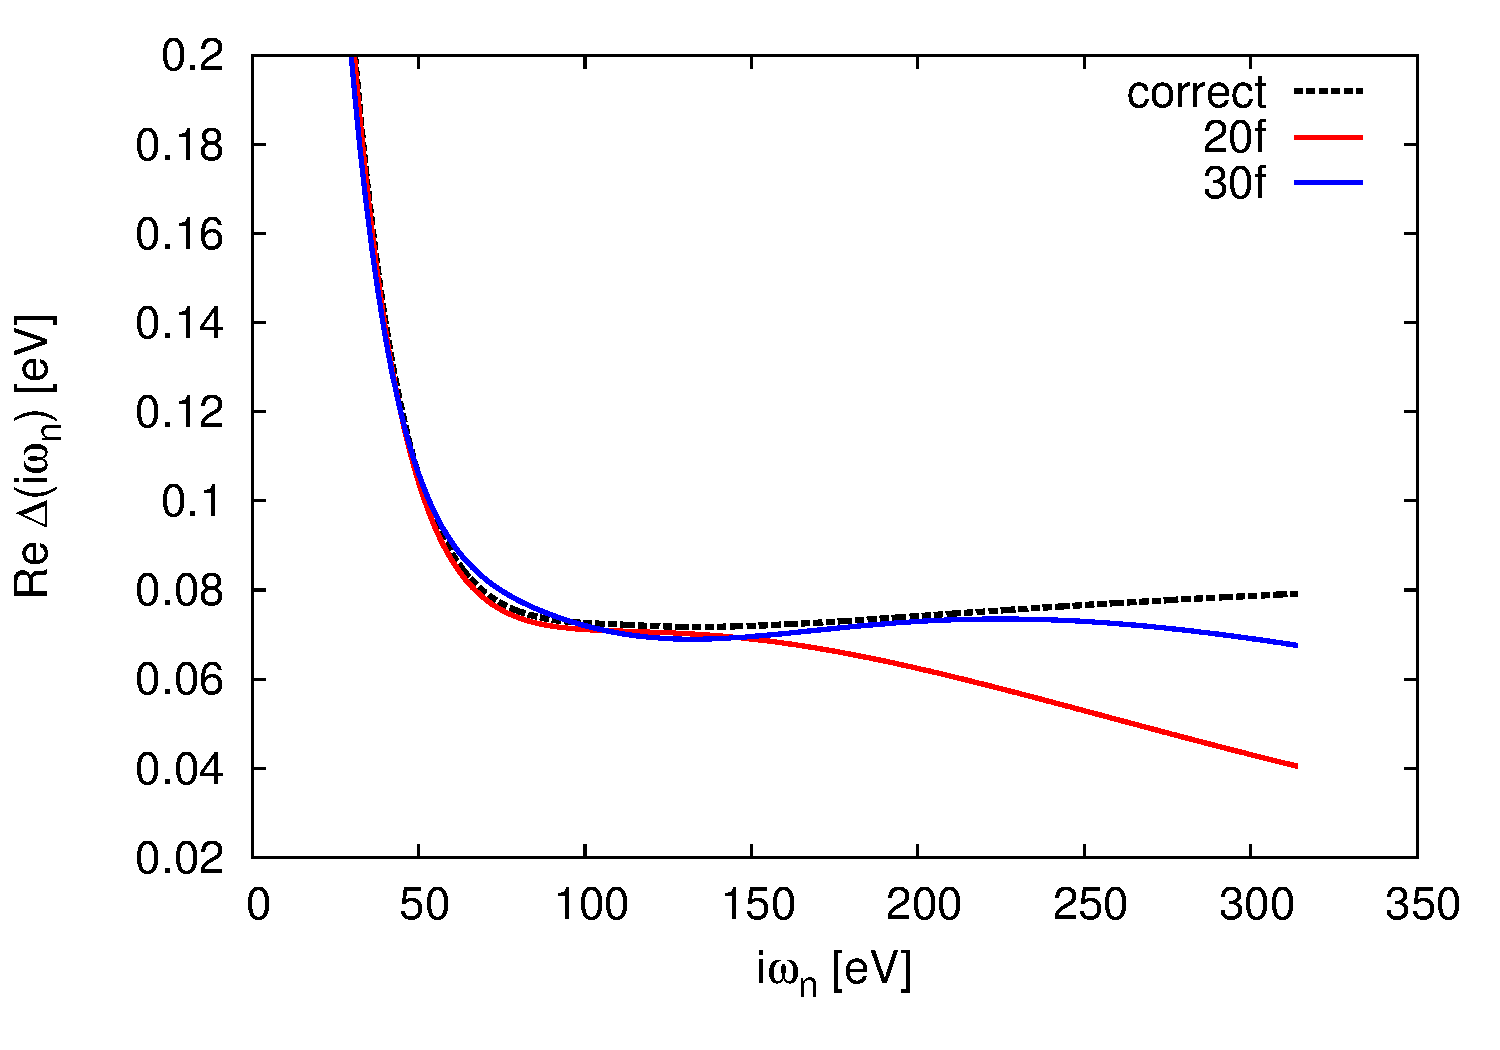
\includegraphics[width=0.6\textwidth]{figs/freqdep/FeSe_hybrid_tail.pdf} 
\end{center}
\caption{This plot shows the real part of the impurty hybridization function
$\Delta(i\omega_n)$ for FeSe, using different frequency grids for the
calculation of the GW Selfenergy. Since the tail of the GW Selfenergy
is usually not well behaved, also the tail of
$\Delta(i\omega_n)$ is usually wrong. For 20 frequencies the tail deviates
very quickly from the correct behaviour, while for 30 
frequencies the deviations sets in later, but still does not allow a proper
high frequency fitting of the tail.}
\label{fig:FeSe_hybrid_tail}
\end{figure}

\textbf{Solution for now}: In principle one should increase the number of
frequencies in the GW calculation, but for this we need at least 60 frequencies
which is impossible right now in terms of calculation time and memory consumption.
Therefore, we fit the GW Selfenergy in a frequency range which is still reliable
but as large as possible with the following form
\begin{align}
\mathrm{Re}\Sigma(i\omega) \sim  c_0 + \frac{c_2}{(i\omega)^2} + \frac{c_4}{(i\omega)^4}
\end{align}
and replace the tail completely by this expression.
In FeSe in Fig.~\ref{fig:FeSe_hybrid_tail} this is the case around $100$~eV,
where we cut all further values and replace them by the fitted expression above.
This is done for all orbital components of the GW Selfenergy at each k-point.

This of course introduces some kind of error, since around $100$~eV
the GW Selfenergy is not sufficiently described by such a term as the one above.
Still, this is probably the better way since the high-frequency tail without 
this treatment would be even more wrong, and would prevent a calculation of 
the impurity levels and $\Delta(\tau)$, as discussed above.



%%%%%%%%%%%%%%%%%%%%%%%%%%%%%%%%%%%%%%%%%%%%%%%%%%%%%%%%%%%%%%%%%%%%%%%%%%%%%%%%%%%%%
%%%%%%%%%%%%%%%%%%%%%%%%%%%%%%%%%%%%%%%%%%%%%%%%%%%%%%%%%%%%%%%%%%%%%%%%%%%%%%%%%%%%%
%%%%%%%%%%%%%%%%%%%%%%%%%%%%%%%%%%%%%%%%%%%%%%%%%%%%%%%%%%%%%%%%%%%%%%%%%%%%%%%%%%%%%
%%%%%%%%%%%%%%%%%%%%%%%%%%%%%%%%%%%%%%%%%%%%%%%%%%%%%%%%%%%%%%%%%%%%%%%%%%%%%%%%%%%%%
%%%%%%%%%%%%%%%%%%%%%%%%%%%%%%%%%%%%%%%%%%%%%%%%%%%%%%%%%%%%%%%%%%%%%%%%%%%%%%%%%%%%%

\clearpage

\section{Preliminary GW+DMFT results}
\subsection{SrVO$_3$}

\begin{figure}[H]
\begin{minipage}{0.5\textwidth}
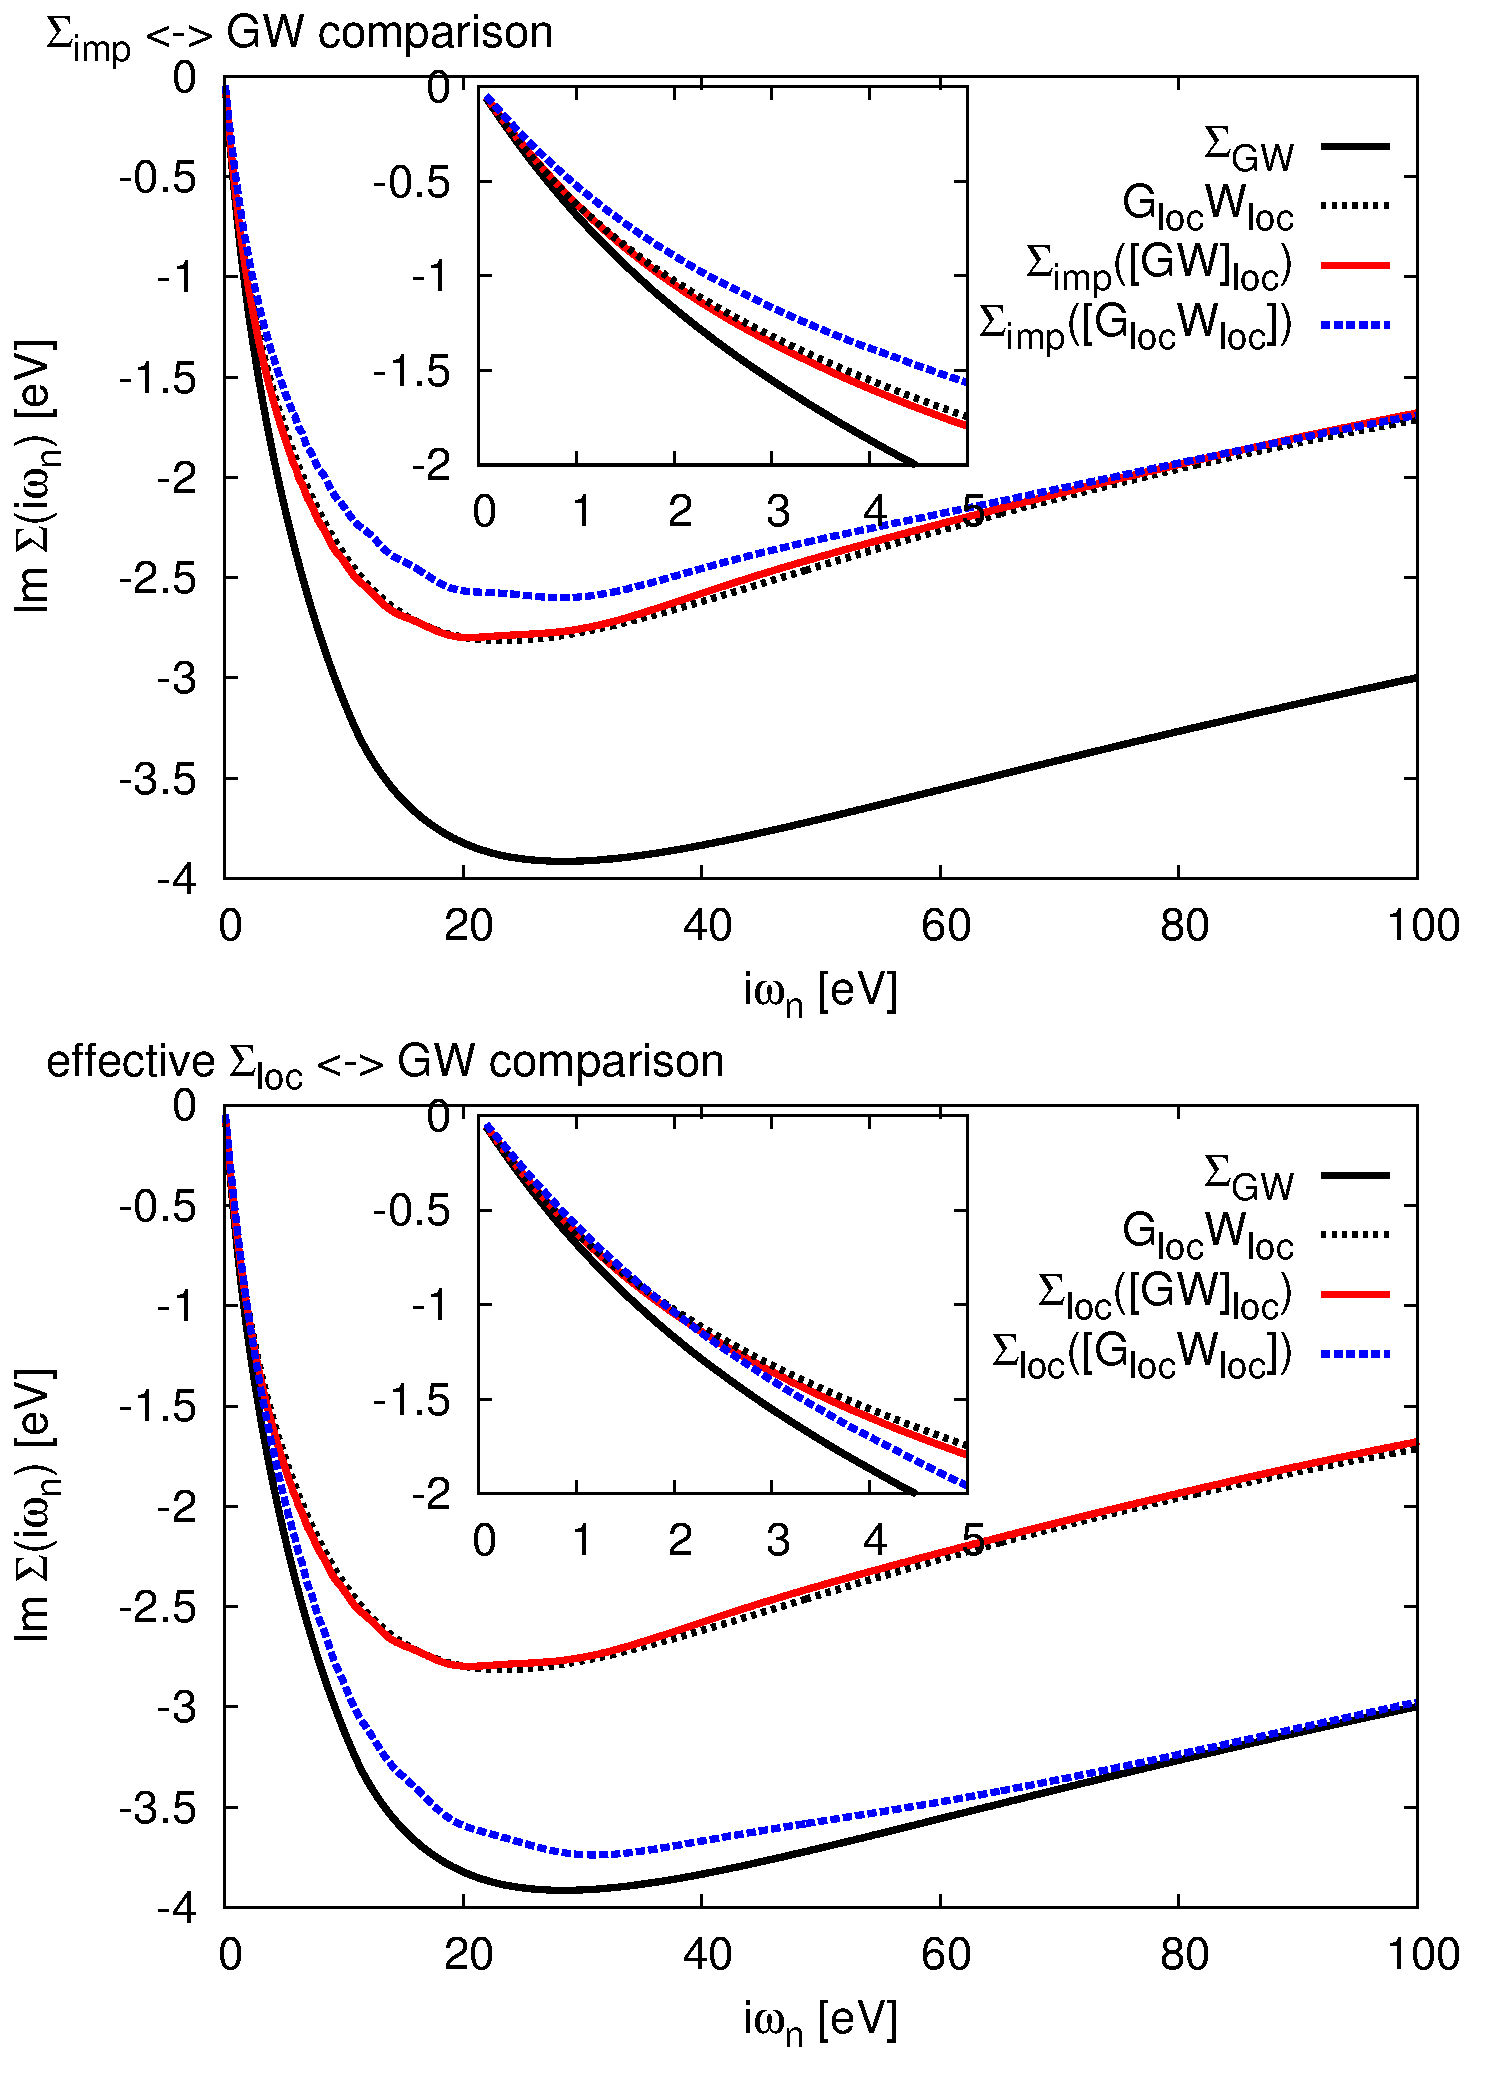
\includegraphics[width=1\textwidth]{figs/results/SrVO3_DC_comparison.pdf} 
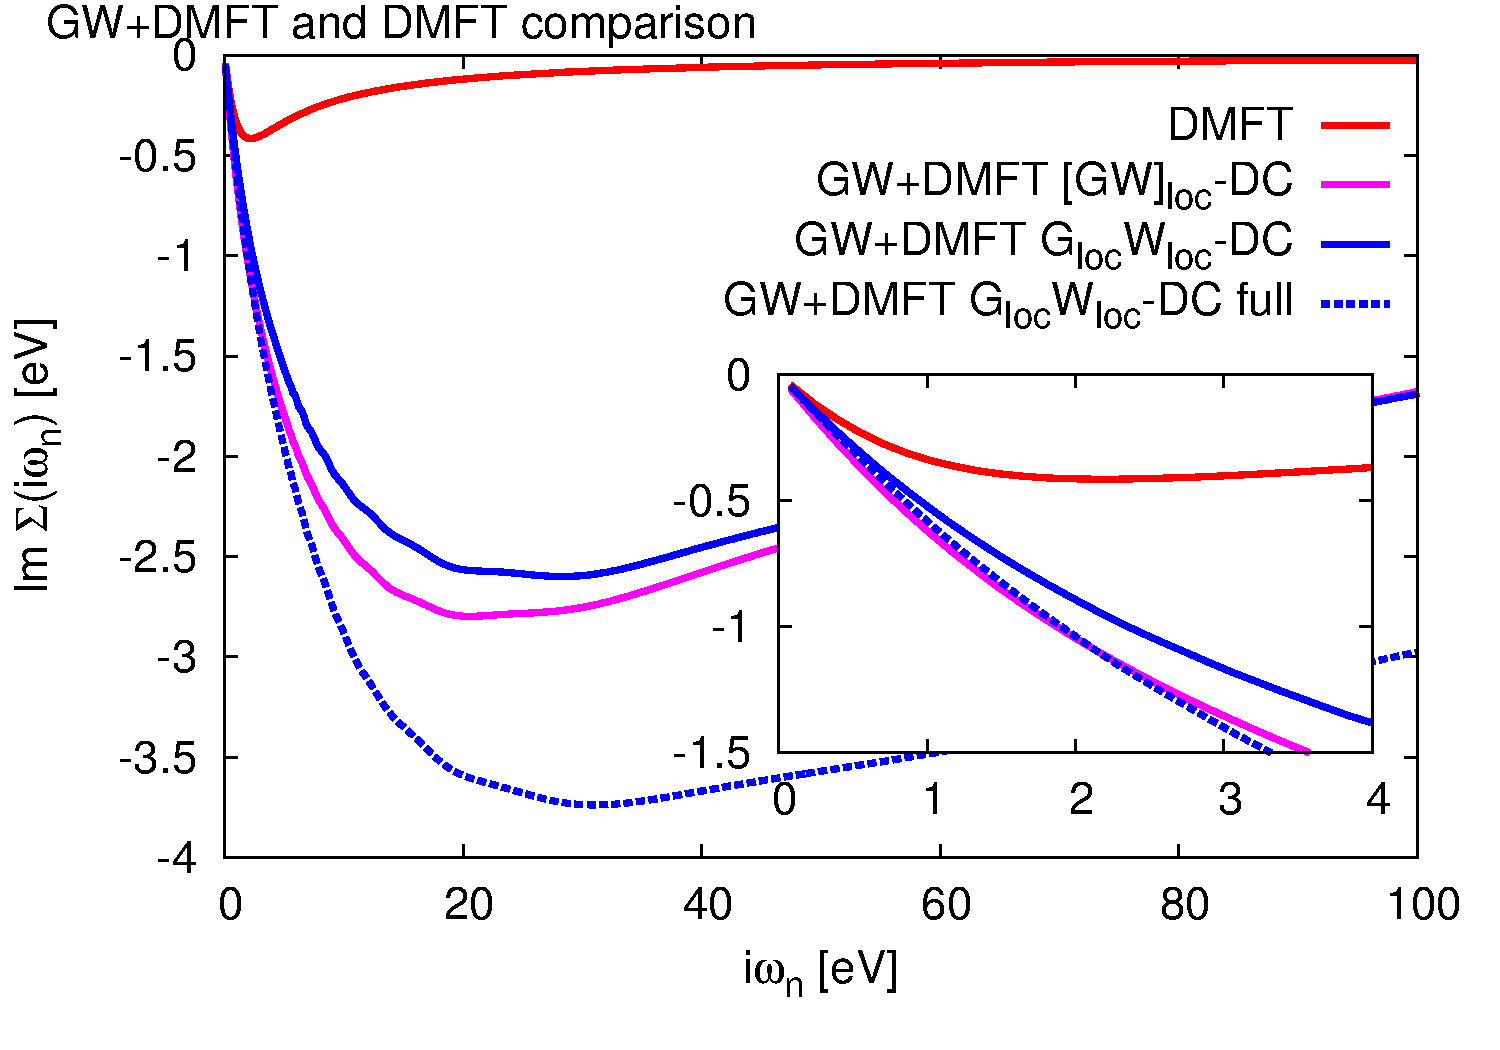
\includegraphics[width=1\textwidth]{figs/results/SrVO3_DC_comparison2.pdf} 
\end{minipage}
\begin{minipage}{0.5\textwidth}
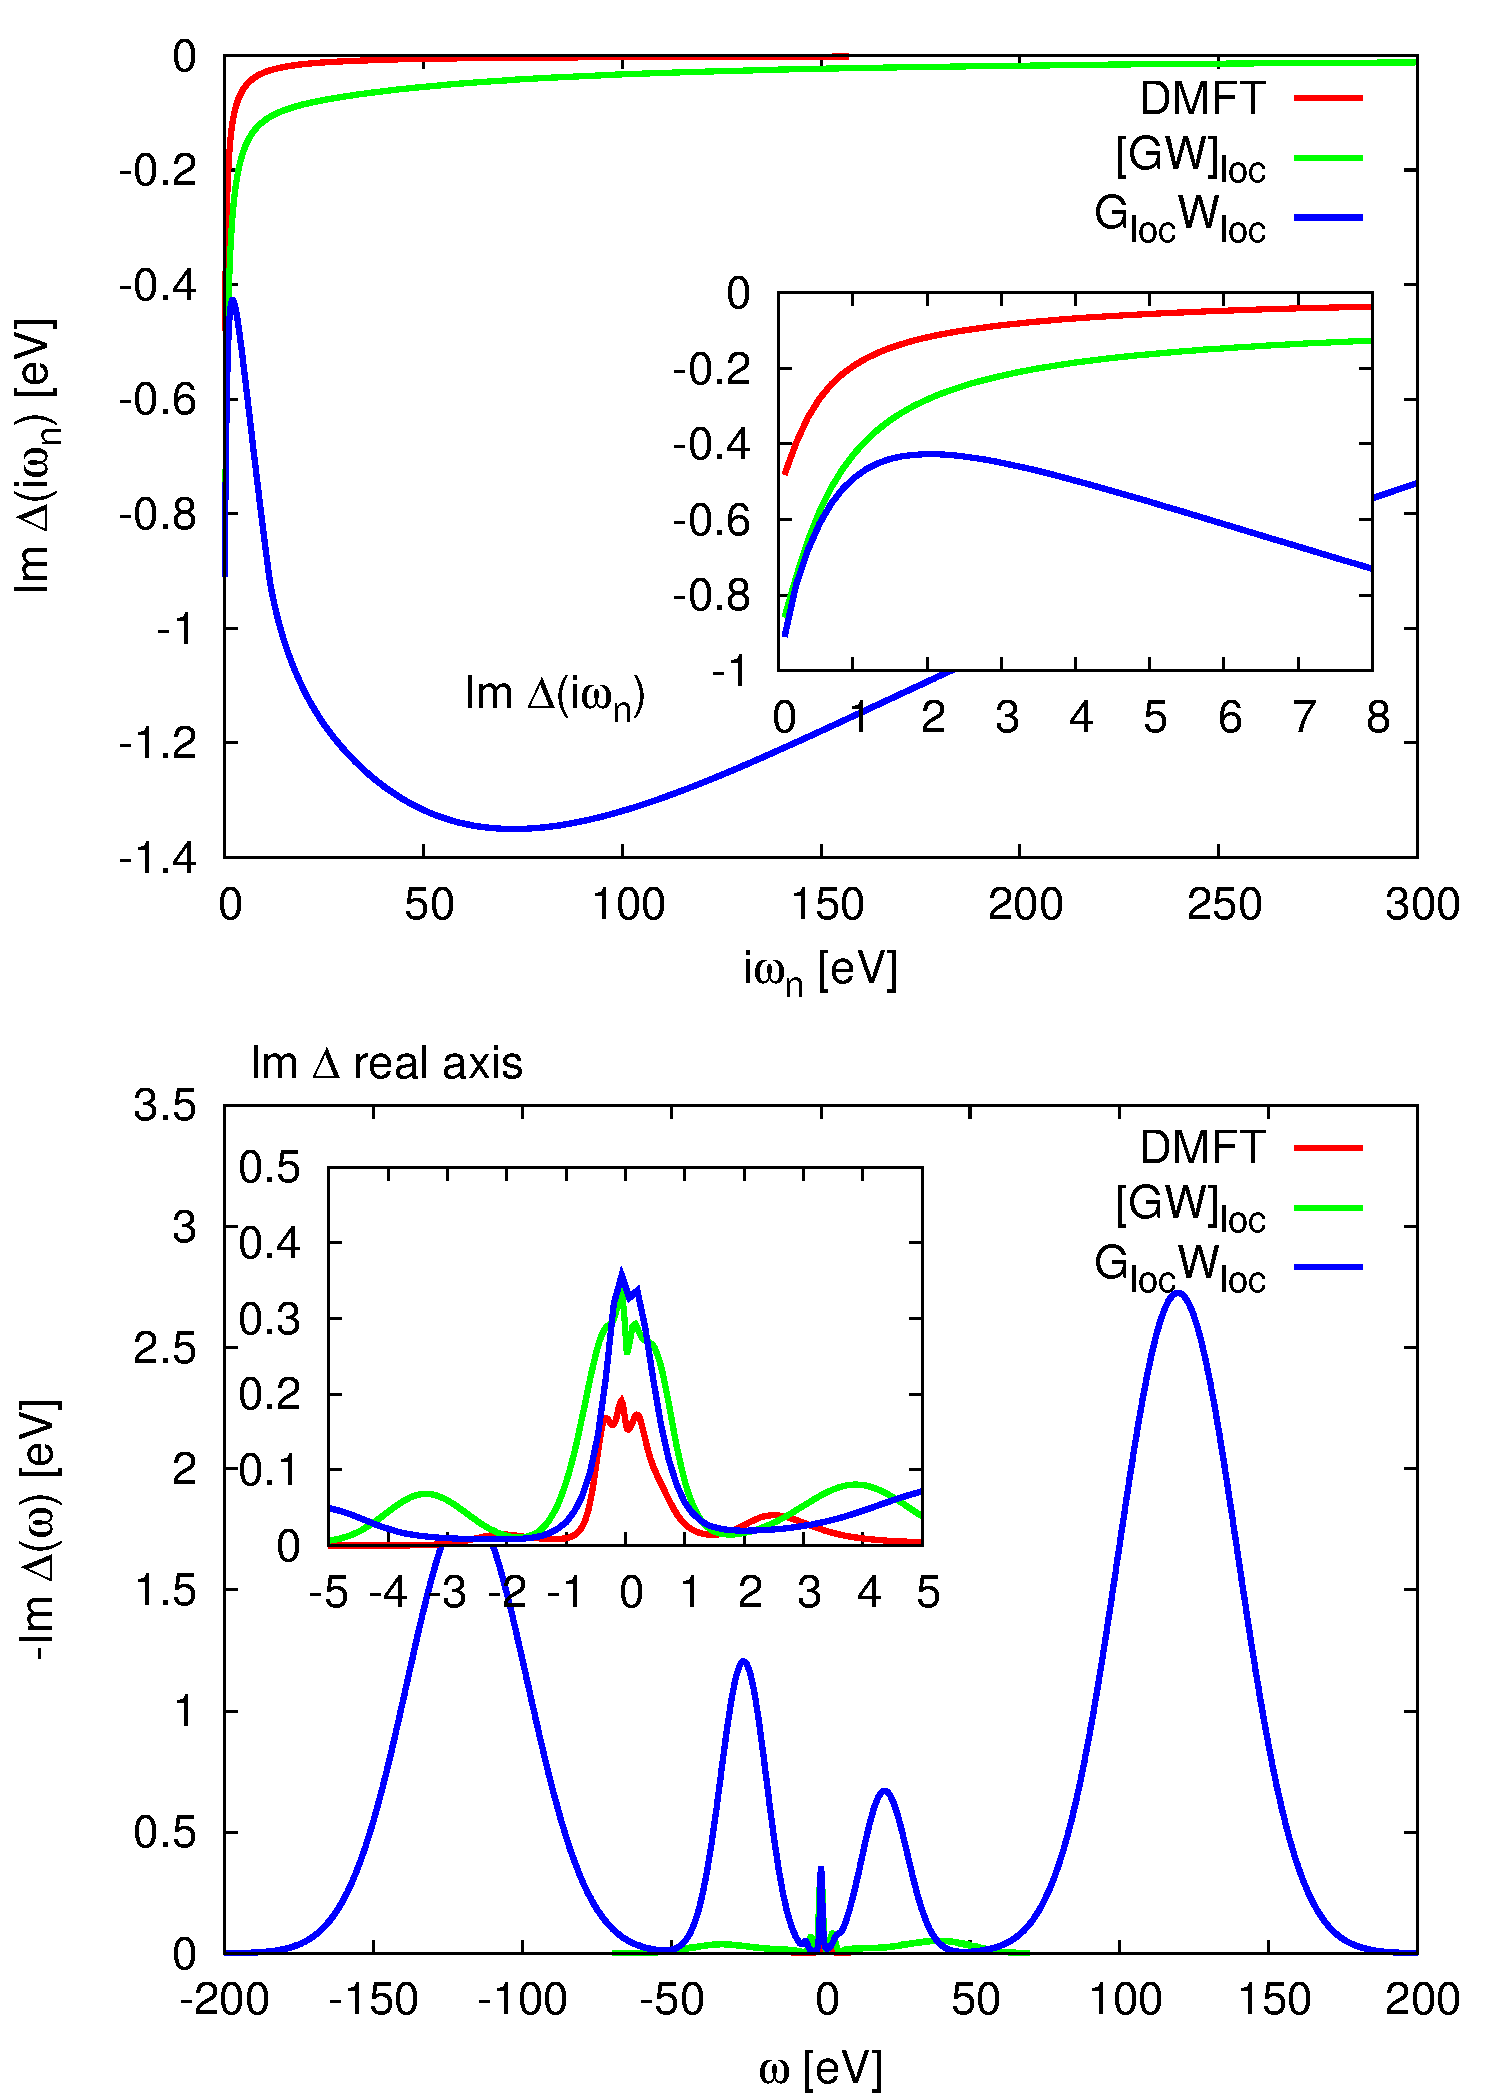
\includegraphics[width=1\textwidth]{figs/results/SrVO3_hybrid_dc_comp.pdf}  
\end{minipage}
\caption{\textbf{Left side}: Comparison of the imaginary part of the local Selfenergy
for GW+DMFT calculations with different doublecountings. The upper plot shows the impurity Selfenergy
for the $[GW]_{loc}$ and the $G_{loc}W_{loc}$ doublecounting, in comparison to the
local GW Selfenergy.\\
The middle plot compares the total local Selfenergies after contributions from
nonlocal propagators from GW have been added.\\
The lower plot compares a standard LDA+DMFT calculation to the two different GW+DMFT 
selfenenergies.\\
\textbf{Right side}:
Comparison of the hybridization function $\Delta$ obtained with the DMFT and the two different GW+DMFT
doublecountings. The upper plot shows $\Delta$ on the imaginary Matsubara axis, the lower
one on the real axis after analytical continuation.}
\label{fig:results_sigma_hybrid_svo}
\end{figure}

\clearpage

\begin{figure}[h]
\begin{minipage}{0.5\textwidth}
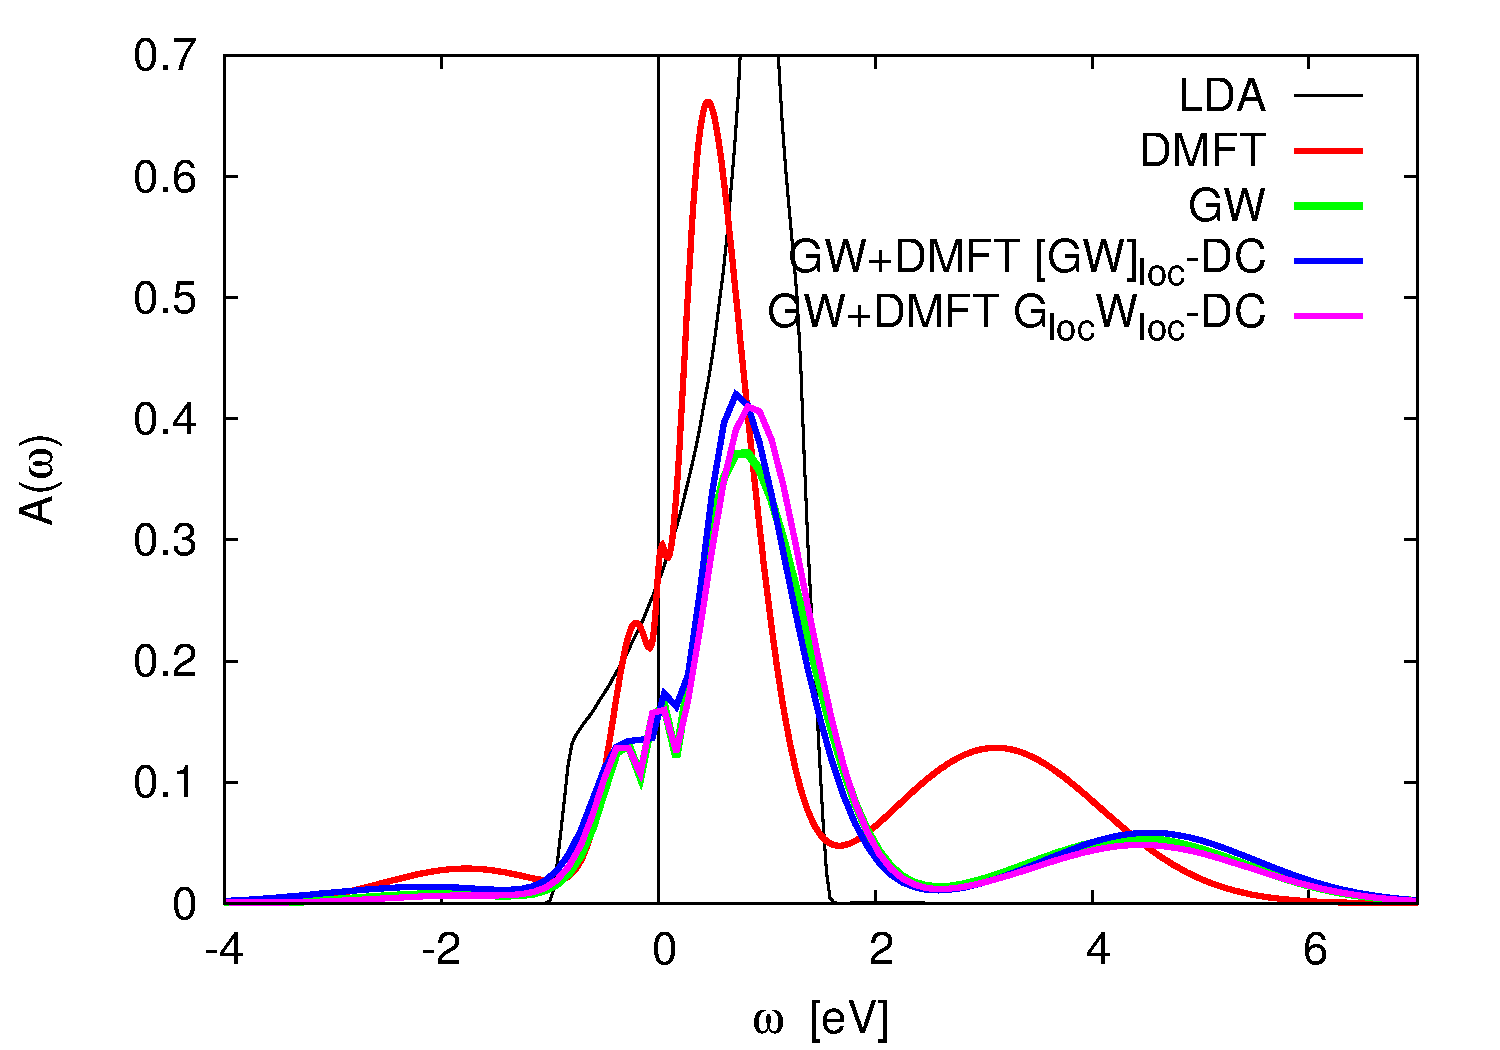
\includegraphics[width=1\textwidth]{figs/results/SrVO3_specFunc_comparison.pdf} 
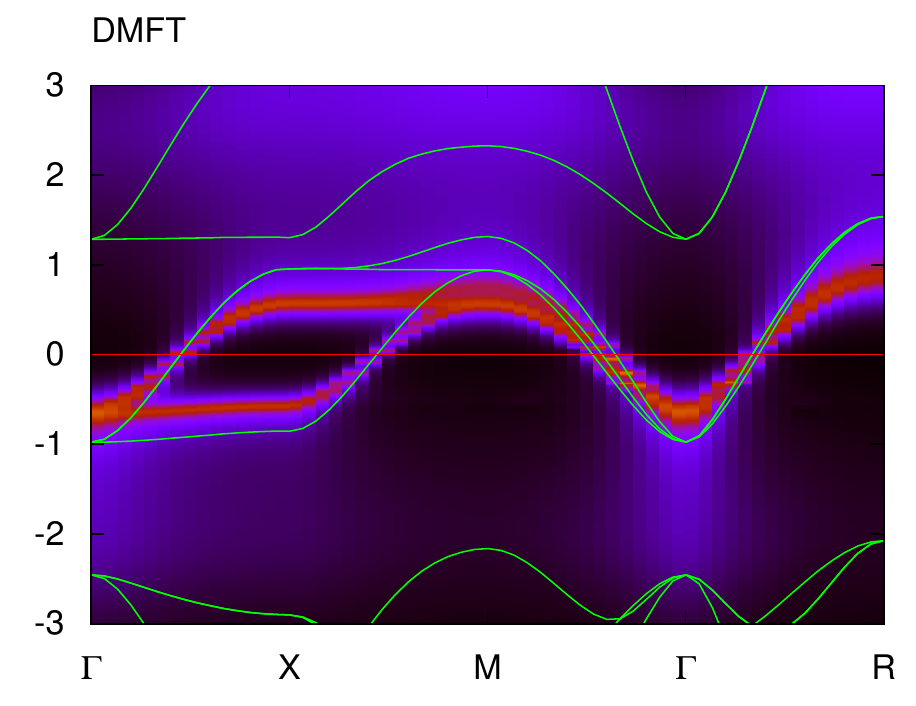
\includegraphics[width=1\textwidth]{figs/results/SrVO3_bands_DMFT.png}  
\end{minipage}
\begin{minipage}{0.5\textwidth}
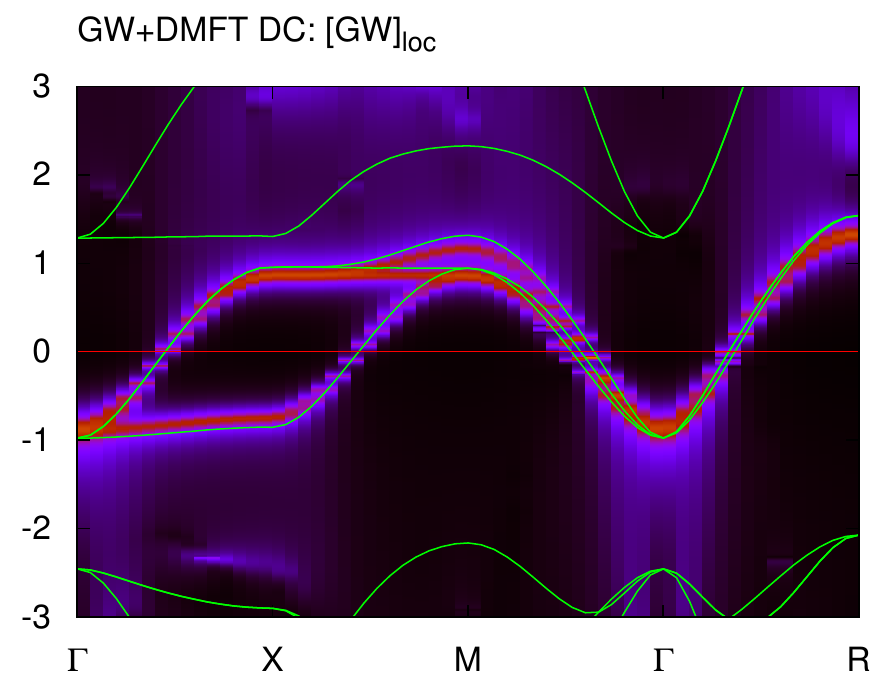
\includegraphics[width=1\textwidth]{figs/results/SrVO3_bands_GWDMFT_gwl.png}  
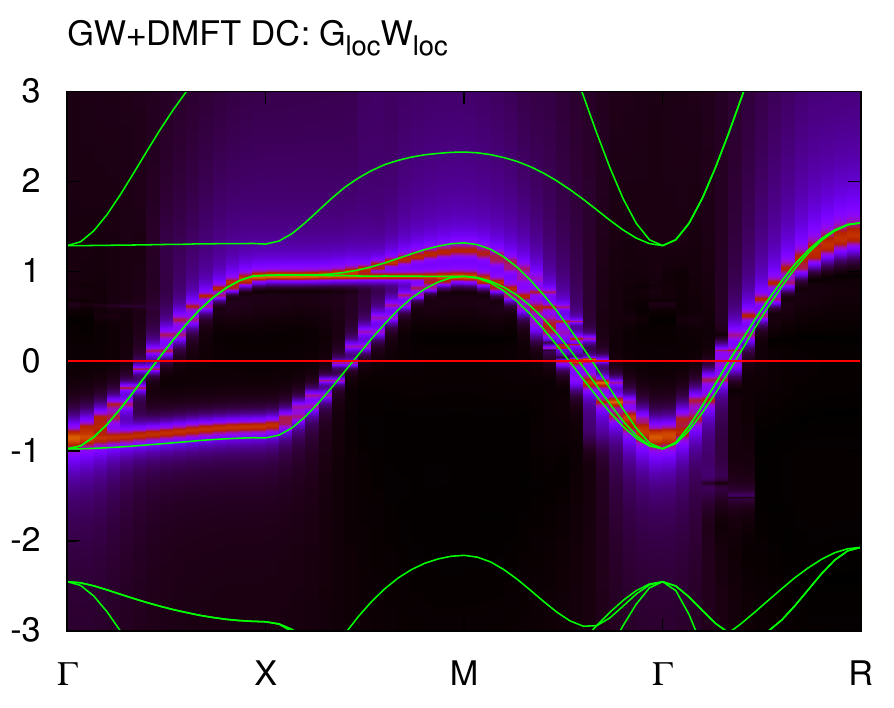
\includegraphics[width=1\textwidth]{figs/results/SrVO3_bands_GWDMFT_glwl.png}  
\end{minipage}

\caption{
\textbf{Upper Left}: The local spectral function of SrVO$_3$, with a comparison
between LDA+DMFT, GW and the two GW+DMFT Doublecountings.\\
\textbf{Lower left, Right}:
The k-resolved spectral function for SrVO$_3$, with a comparison
between LDA+DMFT, GW and the two GW+DMFT Doublecountings.
The green lines show the DFT dispersion}
\label{fig:results_BS_svo}
\end{figure}



\begin{figure}[H]
\begin{center}
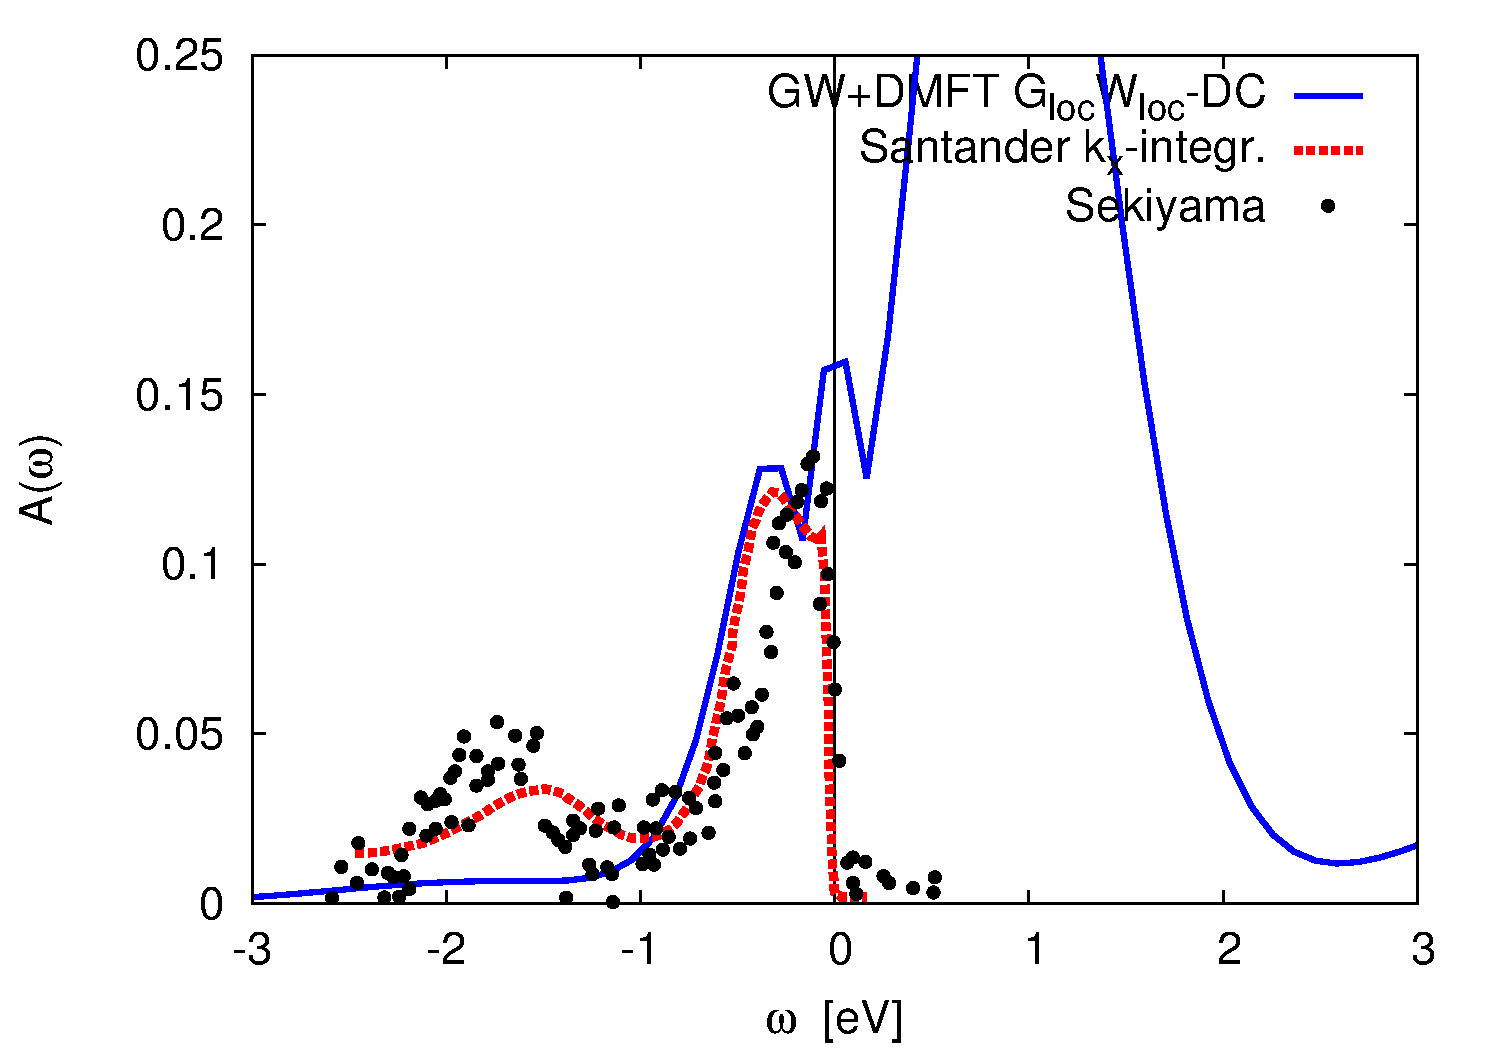
\includegraphics[width=0.7\textwidth]{figs/results/SrVO_spec_ARPES.pdf} 
\end{center}
\caption{
The local spectral function from the GW+DMFT calculation with the 
$G_{loc}W_{loc}$ doublecounting, compared to the PES experiment from Sekiyama,
and from Santander-Syro. The latter has been obtained from ARPES around the 
$\Gamma_{003}$ point and integrated along the $k=\langle 100 \rangle$ direction.}
\label{fig:results_arpes_svo}
\end{figure}


\clearpage

\subsection{Plasmon analysis}

For the investigation of the plasmon and Hubbard satellites in SrVO$_3$
we used the fact that the Hubbard bands are created by the low-energy static
value $U(0)$ of the effective Coulomb interaction,
while the plasmon satellites are created by the frequency dependence
of the interaction $U(\omega)$.

Therefore, we modified the effective bare interaction $U(\omega)$
by subtracting the low-energy static value 
\begin{align}
\tilde{U}_{\alpha}(\omega) &:= U(\omega) - \alpha U(\omega=0),
\end{align}
which allowed us to tune the intensity of the Hubbard bands. If 
$\alpha=0$, there is no modification to the effective interaction
and we obtain both plasmon and Hubbard satellites.
If $\alpha=1$, the effective low-energy static
value $\tilde{U}(0)=0$, so the Hubbard bands vanish and the plasmons
should remain because the frequency dependence of $\tilde{U}(\omega)$
is identical to the original interaction $U(\omega)$.

\bigskip 

Ferdi Aryasetiawan made the interesting comment, that
in principle the plasmons should also be affected, because
the divergencies in the dielectric function $\epsilon(\omega)$
are modified as well
\begin{align}
 \tilde{\epsilon}^{-1}(\omega)
 &= 1 - P(\omega)\tilde{U}_{\alpha}(\omega) \nonumber \\
 &= 1 - P(\omega)\left[  U(\omega) - \alpha U(0) \right] . \label{eq:mod_epsfunc}
\end{align}

To me it is not yet completely clear what this implies in our specific case.
As an example, I have used the effective bare 
interaction $U(\omega)$ for the $t_{2g}$ of SrVO$_3$ calculated in cRPA, 
and calculated the $t_{2g}$ polarization $P(\omega)$ within RPA as $P=G_0G_0$.
Then I calculated $W$ and $\epsilon^{-1}$ by using the formula~\eqref{eq:mod_epsfunc} 
above with the modified interaction $\tilde{U}(\omega)$.

The result is shown in this plot:

\begin{figure}[h]
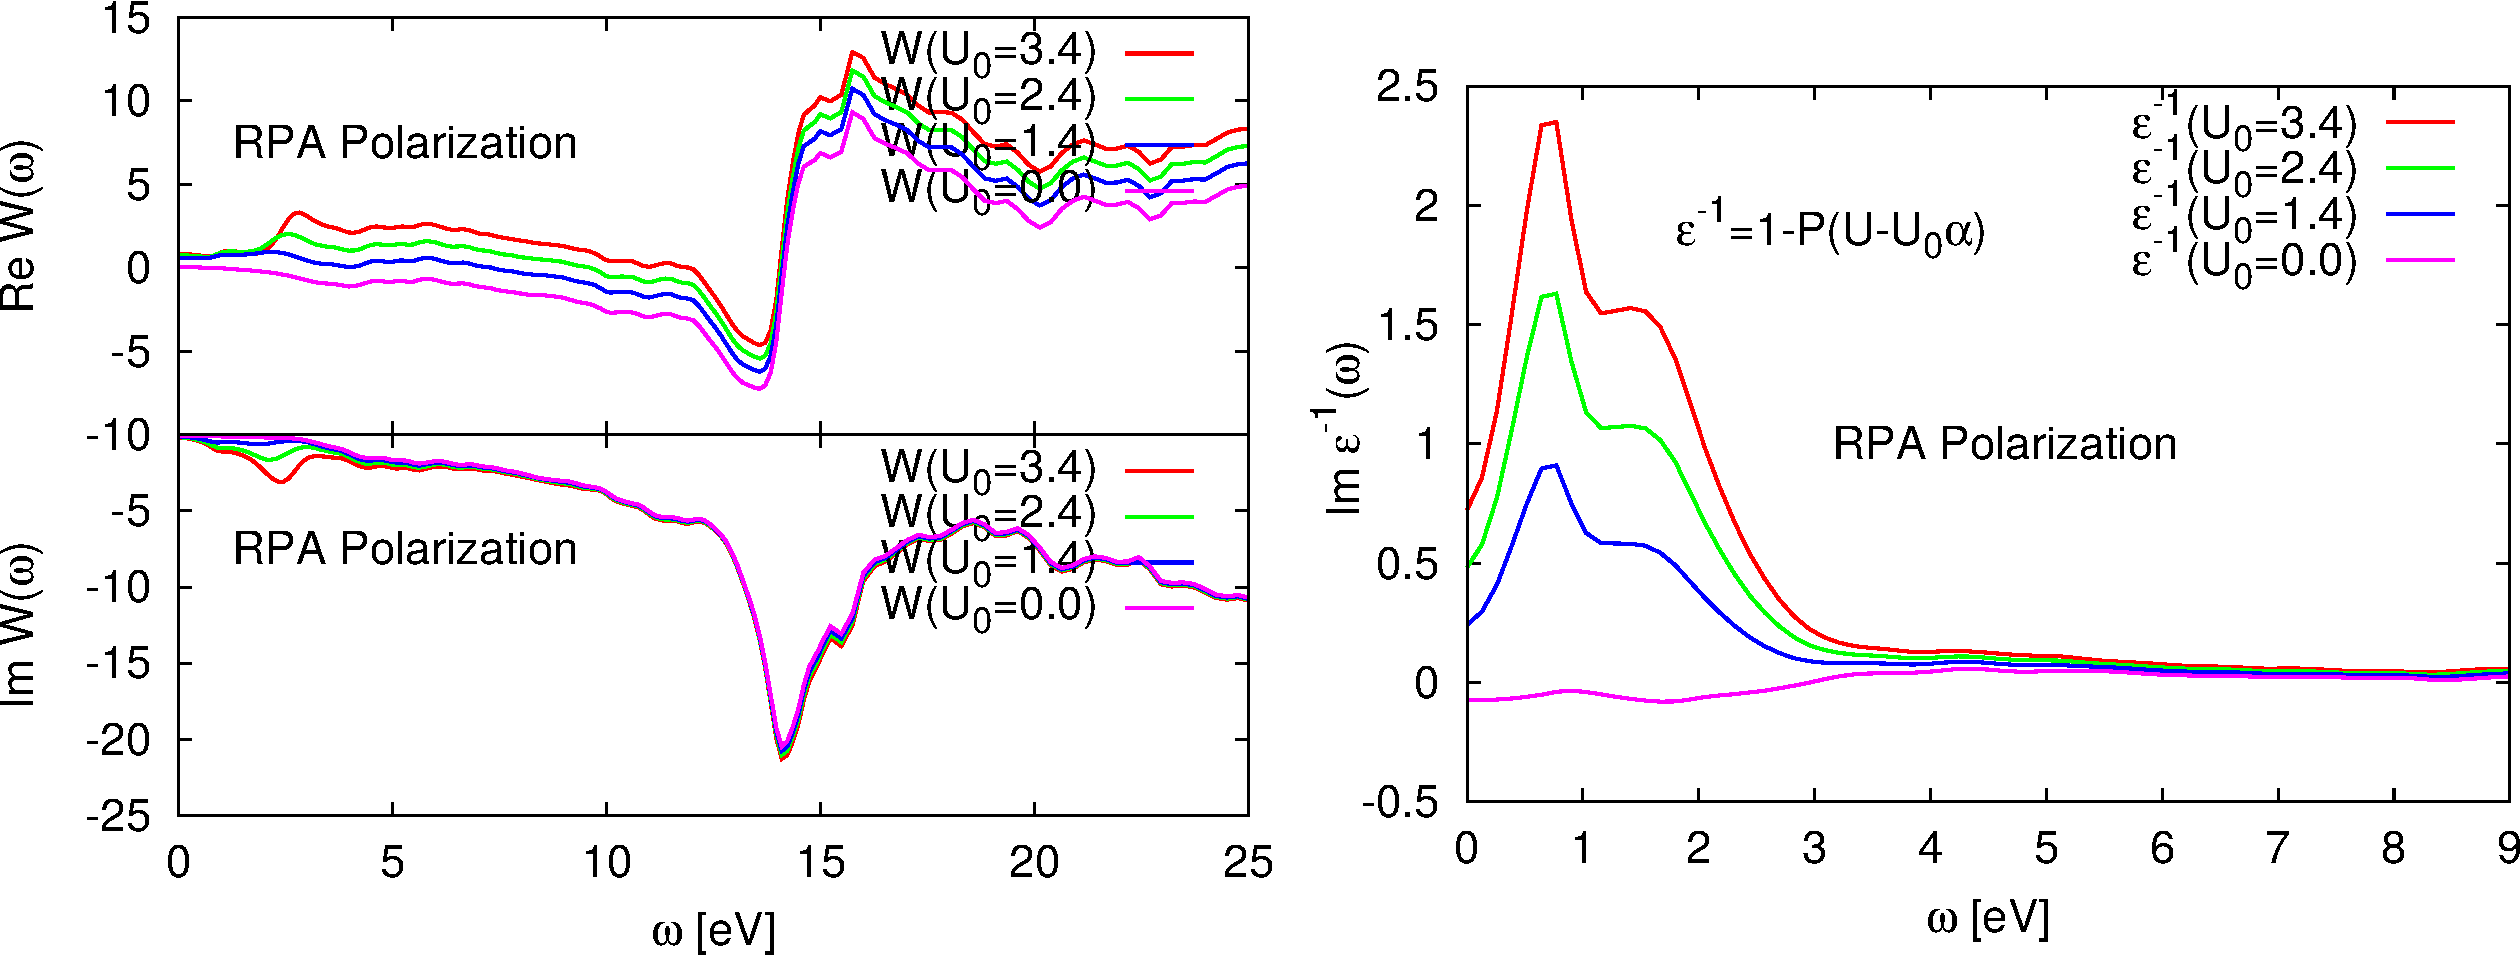
\includegraphics[width=1\textwidth]{figs/plasmonanalysis/modified_UPW.pdf} 
\caption{Left: The screened local Coulomb interaction $W(\omega)$
on real frequencies within the RPA approximation with a modified
effective bare interaction $U(\omega)-\alpha U(0)$ for SrVO$_3$.\\
Right: The inverse of the dielectric function calculated in the same way.
}
\end{figure}

We see that for the original interaction $U(\omega)$ there is
a feature around $2$~eV in the screened interaction $W(\omega)$.
For the reduced interaction all low energy features vanish, 
and the dielectric function Im$[\epsilon^{-1}]$ is featureless.
This indeed would indicate that no low-energy plasmons should exist.

One thing that has to be considered is that the polarization $P(\omega)$
is not modified, because it has been calculated from RPA as $P=G_0G_0$.
If the interaction $U(\omega)$ is modified, the resulting
interacting polarization will also be affected, but this effect
is not taken into account here.

Therefore, we calculated the local polarization $P_{imp}$
from the impurity model from the convered GW+DMFT cycle for SrVO$_3$,
which has been done seperately for every value of the reduced
effective interaction $\tilde{U}(\omega)$.


These are the results: 
On the left side the results are given on the Matsubara axis, while on the right
side they are given on the real frequency axis, by using the Pade approximation (very unreliable!):

\begin{figure}[h]
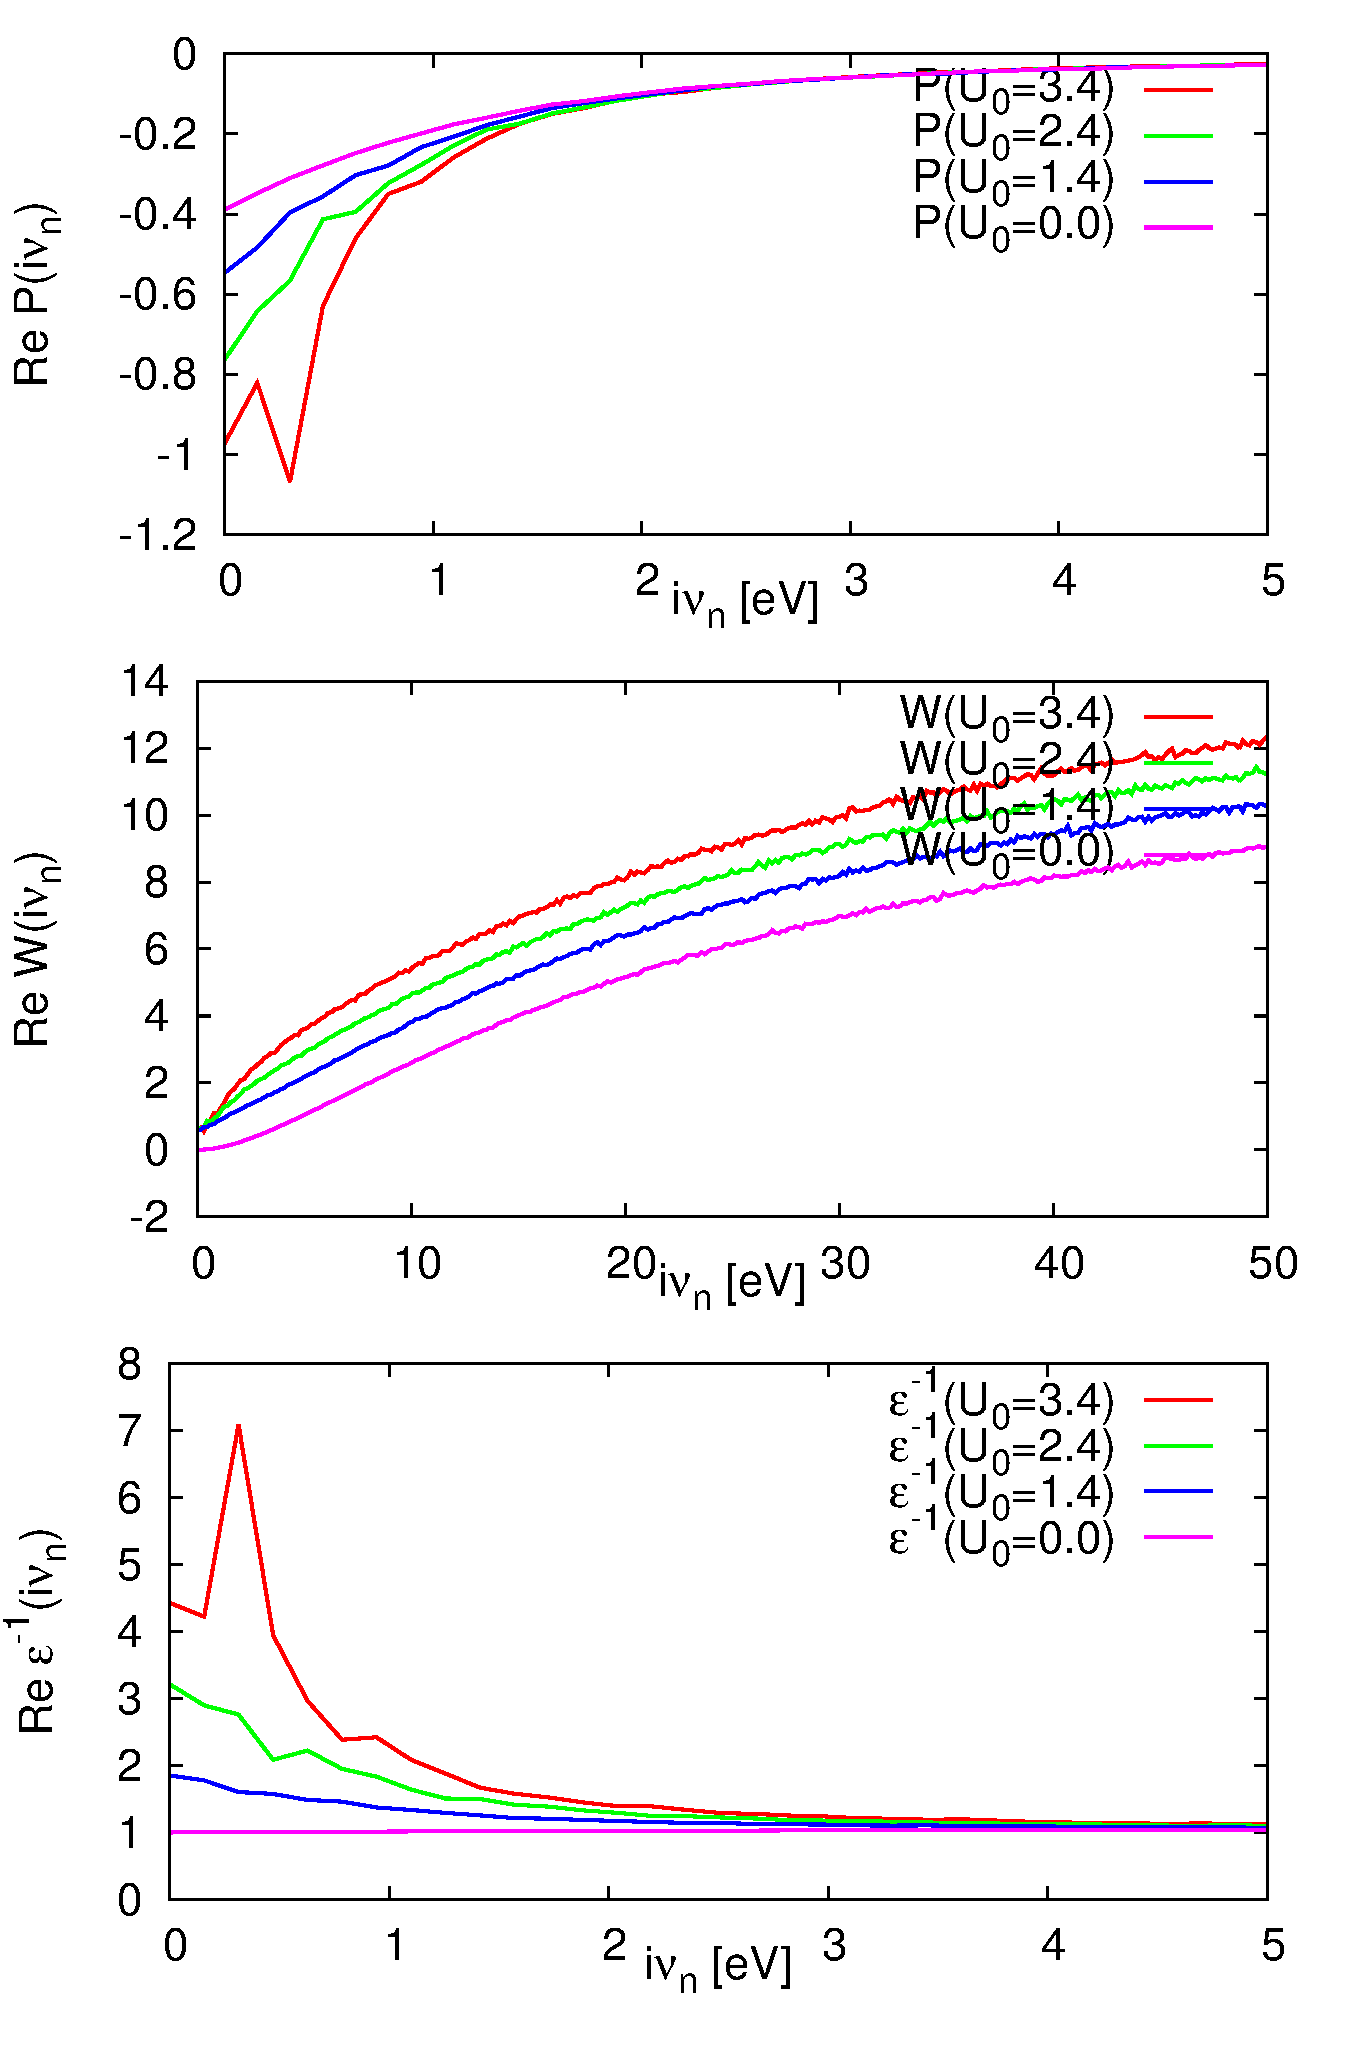
\includegraphics[width=0.5\textwidth]{figs/plasmonanalysis/pol.pdf} 
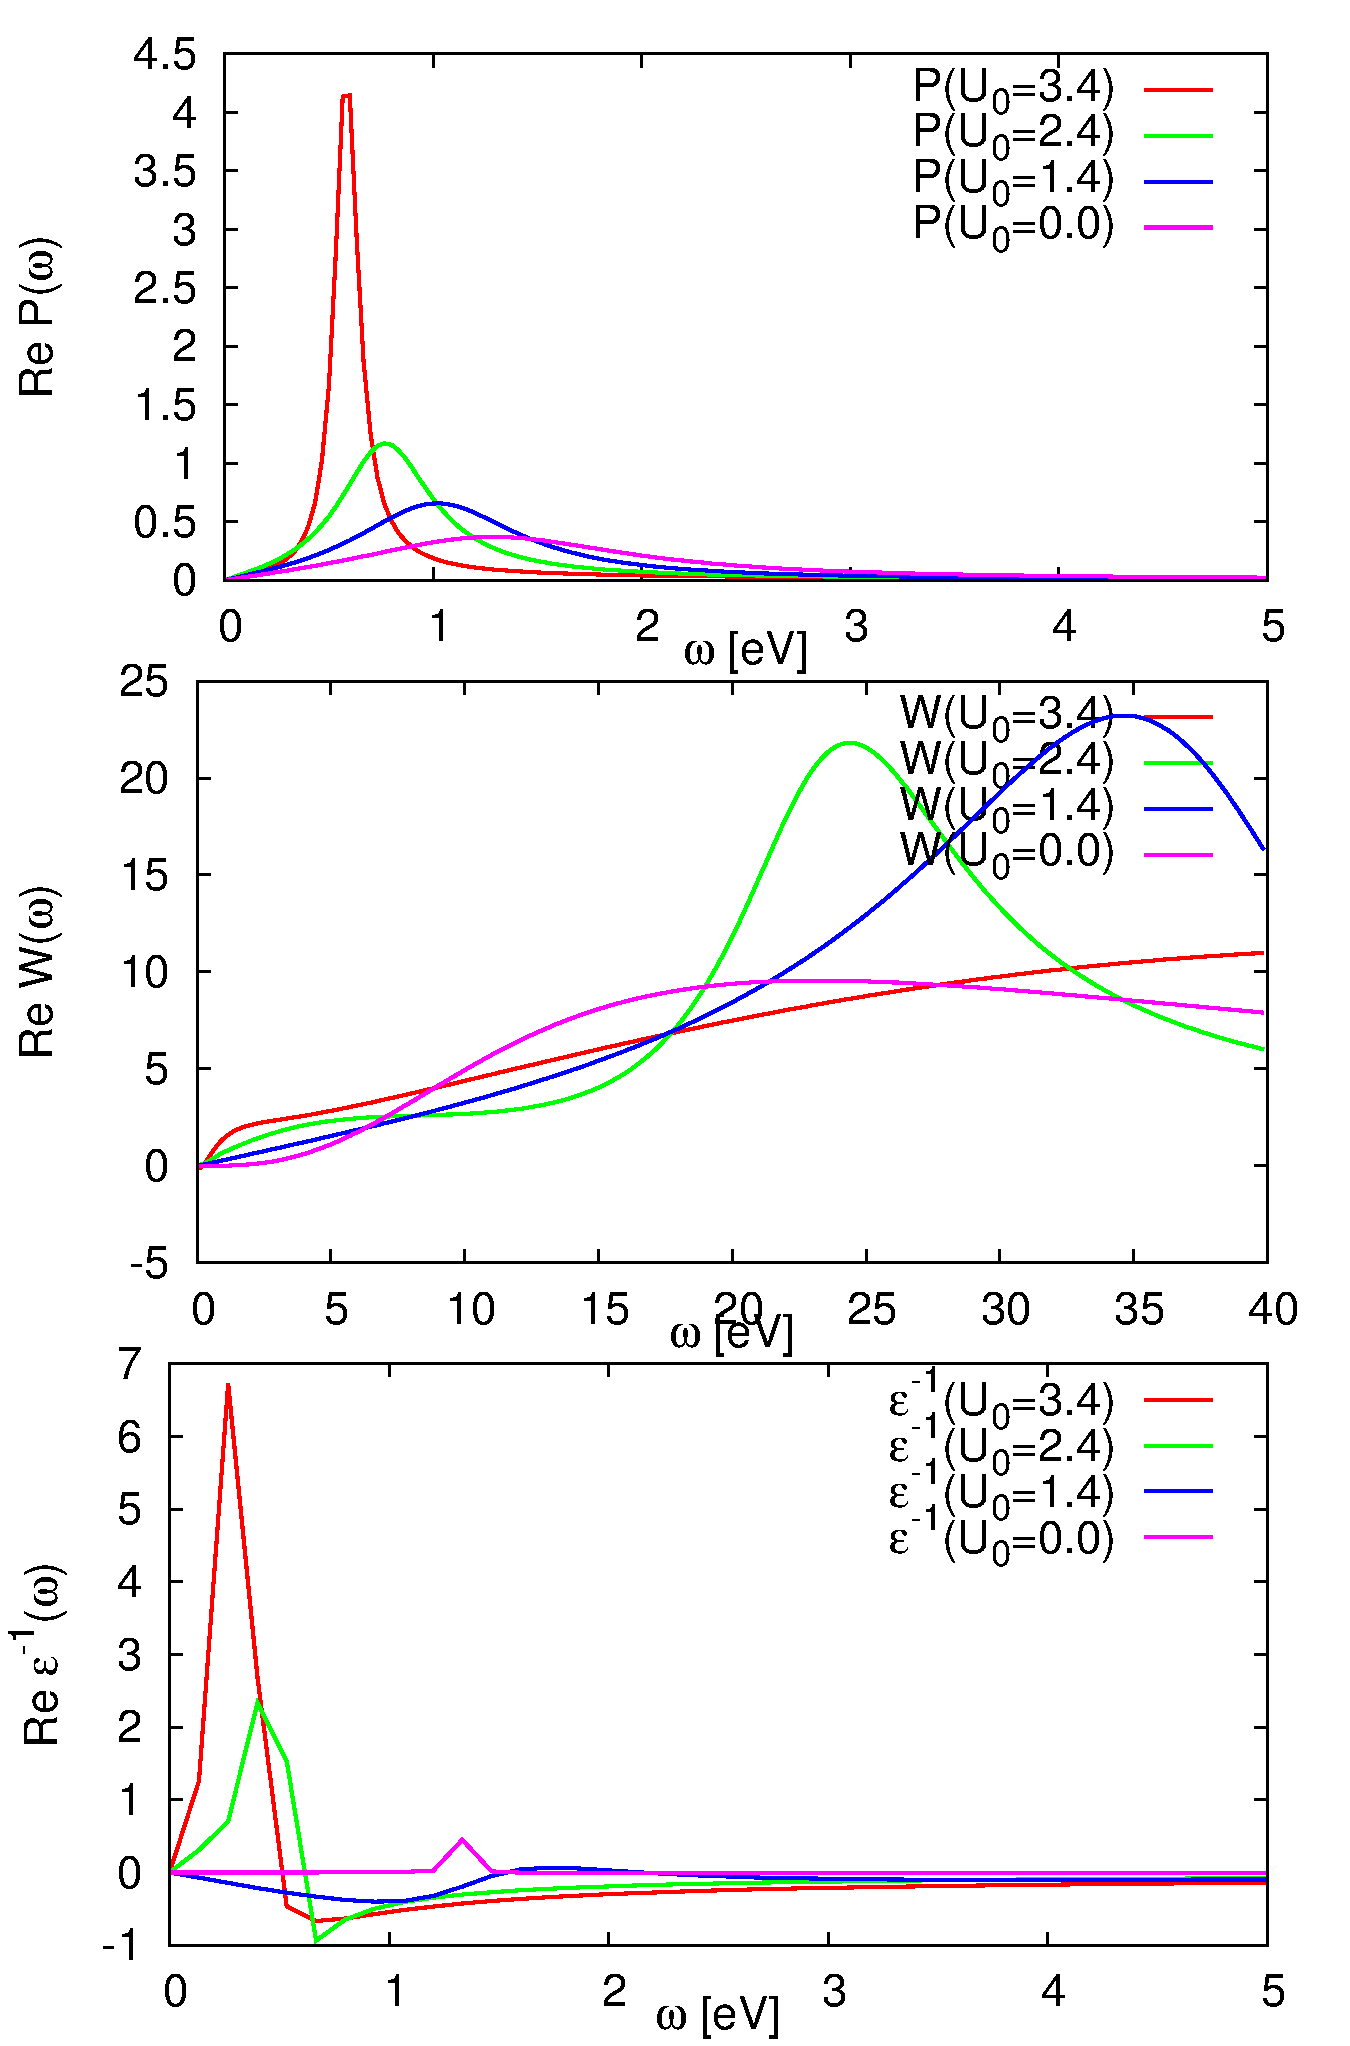
\includegraphics[width=0.5\textwidth]{figs/plasmonanalysis/pol_pade.pdf} 
\caption{Left: The impurity polarization $P_{imp}(i\nu_n)$
for different values of the effective interaction $\tilde{U}(i\nu_n)$ ,
as well as the screened local Coulomb interaction $W(i\nu_n)$
and the inverse of the dielectric function $\epsilon^{-1}(i\nu_n)$
on imaginary Matsubara frequencies. They have been calculated from 
the converged GW+DMFT calculation with the corresponding modified $\tilde{U}$.\\
Right side:
The same objects but calculated on the real frequencie axis
by using the Pade approximation for analytic continuation. (very unreliable! I dod not manage to
perform a Maxent analytic continuation...).
}
\end{figure}

We basically observe the same effect as in the previous RPA results:
the polarization $P$, screened interaction $W$ and dielectric function 
$\epsilon^{-1}$ become featureless when the low-energy static value of $U(\omega)$
is reduced, even when the frequency dependence is not modified.
The kinks visible in the data are numerical noise from the QMC calculation.

Still, in the spectral function of SrVO$_3$ we see that there are
satellite peaks remaining even when $U(0)=0$. 
In the one-orbital model calculation we could also show
that when reducing the $U(0)$ value but keeping the frequency dependence, 
the plasmons in the spectral function are basically
unaffected.
So how can these two seemingly contradictory observations be reconciled?

I think that the point here is that the calculations are not selfconsistent 
in the interaction $W$ resp. $U$.
The resulting polarization $P$ and screened interaction $W$
are of course affected, and they show no plasmonic low-energy features, but
still the effective $\tilde{U}(\omega)$ does, because it is not
updated self-consistently. 
At this point we actually do not want to and also cannot 
calculate $U$ self-consistently, because we manually set it to a different value.
I think it does not make sense to analyze the existence of plasmons by looking
at $P,W,\epsilon$ calculated in this way, because they can only give us 
an answer about the existence of plasmons when they are selfconsistent.

Therefore, I think the analysis of the one-orbital model in our 
Plasmon-Hubbard paper is the right way to check whether plasmons 
are affected by reducing the $U(0)$ value. And this analysis
has shown that they are \textit{not} affected.
So I think our plasmon-hubbard paper is fine, 
but I am not sure how to formulate the final answer to 
Ferdi's remark...

\clearpage



\subsection{FeSe}
\begin{figure}[h]
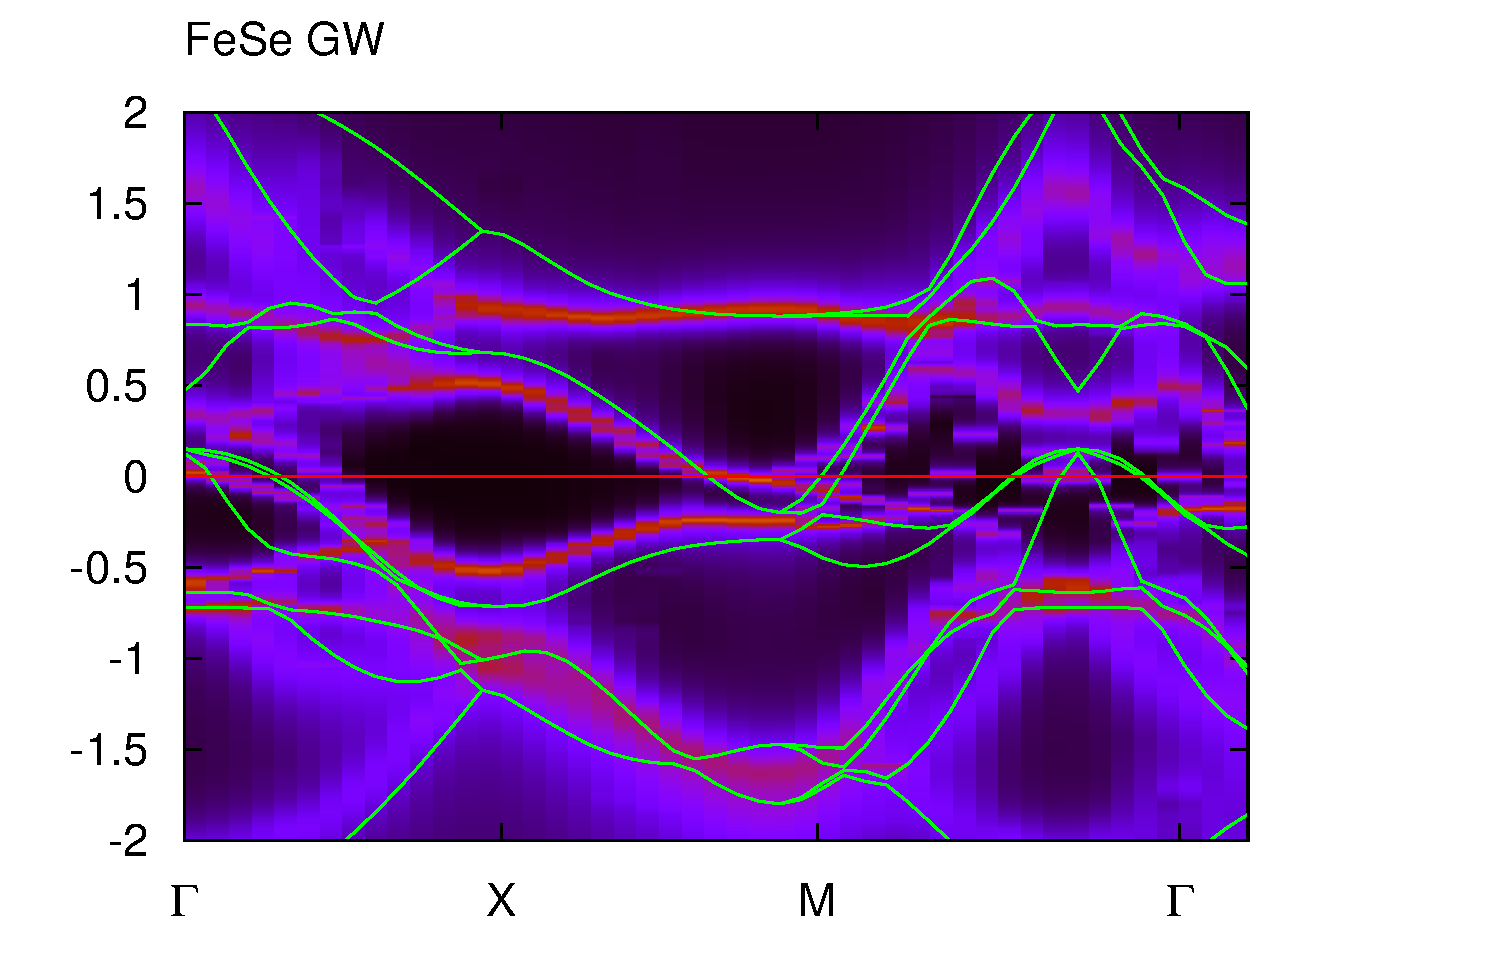
\includegraphics[width=1\textwidth]{figs/results/FeSe_bands_GW.pdf} 
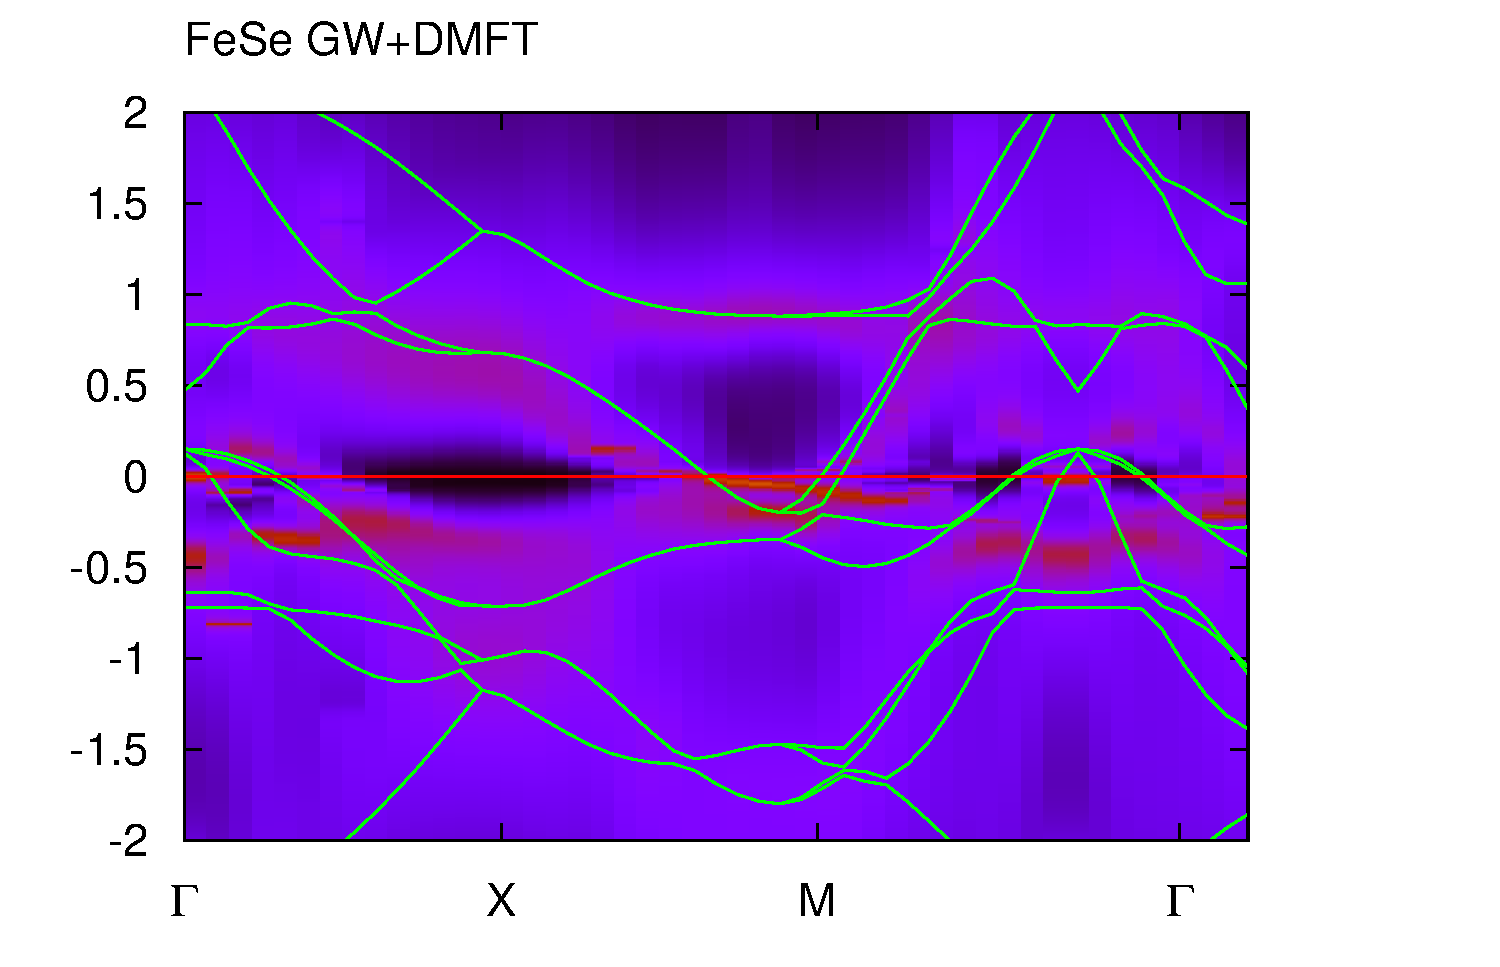
\includegraphics[width=1\textwidth]{figs/results/FeSe_bands_GWDMFT.pdf} 

\vspace*{-0.5cm}
\caption{Top: The spectral function for FeSe within $G_0W_0$.\\
Bottom: The spectral function for FeSe within GW+DMFT,
using the $G_{loc}W_{loc}$ doublecounting and the full orbital dependent 
non-Slater interaction matrix from cRPA. The green lines show the DFT dispersion.
}
\label{fig:results_BS_fese}
\end{figure}

\clearpage


\subsection{NiO}
\begin{figure}[h]
\begin{center}
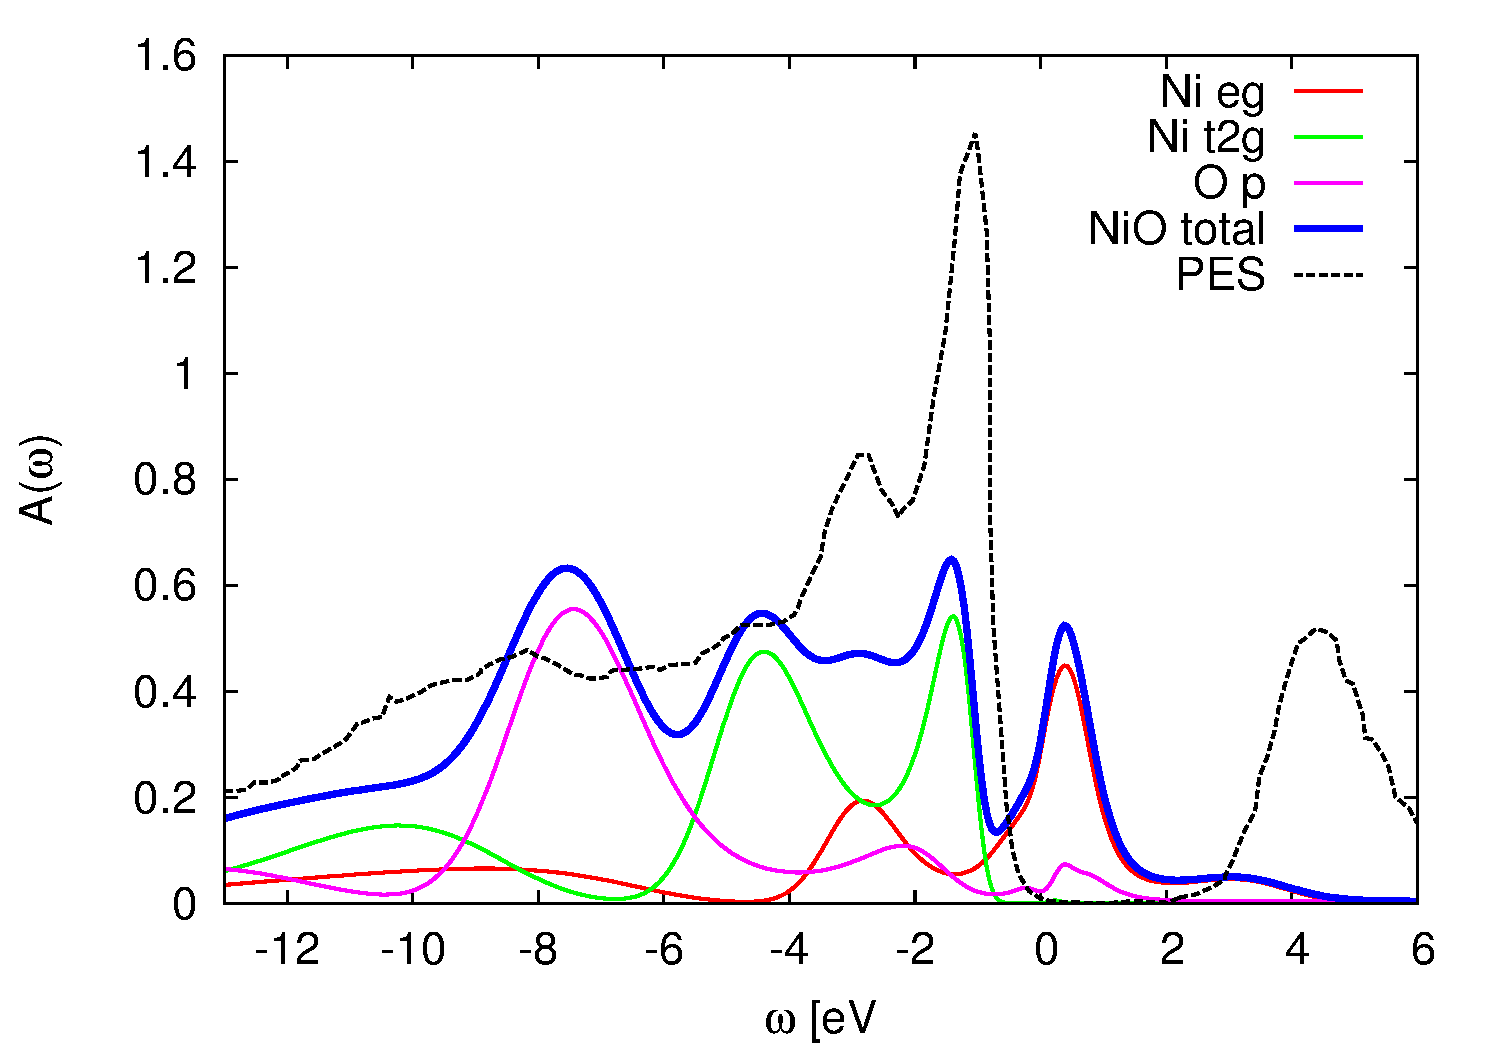
\includegraphics[width=1\textwidth]{figs/results/NiO_dos.pdf} 
\end{center}
\caption{The local spectral function for NiO within GW+DMFT,
using a dp model, compared to PES experiment.}
\label{fig:results_DOS_nio}
\end{figure}

Well, this doesn't look so bad for the first try of
doing GW+DMFT for a d-p model.
Unfortunately the eg's are not insulating...


\clearpage
%%%%%%%%%%%%%%%%%%%%%%%%%%%%%%%%%%%%%%%%%%%%%%%%%%%%%%%%%%%%%%%%%%%%%%%%%%%%%%%%%%%%%
%%%%%%%%%%%%%%%%%%%%%%%%%%%%%%%%%%%%%%%%%%%%%%%%%%%%%%%%%%%%%%%%%%%%%%%%%%%%%%%%%%%%%
%%%%%%%%%%%%%%%%%%%%%%%%%%%%%%%%%%%%%%%%%%%%%%%%%%%%%%%%%%%%%%%%%%%%%%%%%%%%%%%%%%%%%
%%%%%%%%%%%%%%%%%%%%%%%%%%%%%%%%%%%%%%%%%%%%%%%%%%%%%%%%%%%%%%%%%%%%%%%%%%%%%%%%%%%%%
%%%%%%%%%%%%%%%%%%%%%%%%%%%%%%%%%%%%%%%%%%%%%%%%%%%%%%%%%%%%%%%%%%%%%%%%%%%%%%%%%%%%%




\section{Implementation details}

\subsection{Impurity solver input}

The CT-HYB impurity solver by Yusuke needs the following input files
\begin{description}
\item[dmft.input] Includes information about U,J, number of frequencies, etc. At the moment
possible: Only 3-fold degenerate orbitals. No freq. dependent U.

\item[hyb\_tau.dat] The hybridization function as a matrix for imaginary time. 
It needs to be diagonal! \\
Only real part, one column. Seperate matrix elements
via two line breaks and \verb|# hyb     2    1| etc. We need \verb|Nmesh+1|
points where the endpoints $\tau=0,\beta$ are included! By convention has negative sign.
\cng{The local orbital levels are assumed to be $\tilde{\mu}=0$ and any
shift is absorbed in the chemical potential! This has to 
be checked for consistency!!!}

\item[omega\_mesh.dat] Specifies the bosonic frequency grid for some 
correlation functions. Just reuse the standard template file. Not important for us.

\item[fort.10*] Includes information about the Monte-Carlo configuration used
for starting the sampling. Is initialized once with Yusuke's code and then overwritten by 
the solver. No change required here.
\end{description}

\clearpage

\subsection{Bandstructure calculation}
All data in the GW+DMFT calculation is given on the imaginary Matsubara frequency axis. To obtain 
the Bandstructure on real frequencies, we proceed as follows:
\begin{enumerate}
\item First, we create the Green's function for a given $k$-point on the Matsubara axis via
\begin{align}
 G(k,i\omega_n) 
 &= \left[ \unity(i\omega_n+\mu ) -H^{DFT}(k) + v^{XC}(k) \right. \nonumber \\
          & \hspace{1cm}- \Sigma^{GW}(k,i\omega_n) 
          + \Sigma^{GW,loc}(i\omega_n)
          \left. - \Sigma^{imp}(i\omega_n)
           \right]^{-1} 
%
\end{align}
Or, for example, to obtain only the GW Bandstructure we set the impurity contributions to zero
\begin{align}
 G(k,i\omega_n) 
 &= \left[ \unity(i\omega_n+\mu ) -H^{DFT}(k) + v^{XC}(k) \right. \nonumber \\
          &\left. \hspace{1cm}- \Sigma^{GW}(k,i\omega_n) 
           \right]^{-1} 
%
\end{align}
Then the Pade-approximation is applied to $G(k,i\omega_n) $ to obtain $G(k,\omega) $ on the real axis.
This is done for all k-points.
The spectral function is then given by
\begin{align}
A(k,\omega) = -\frac{1}{\pi} \mathrm{Im}G(k,\omega)
\end{align}

\end{enumerate}


\end{document}
